%============================================================
%  CHAPTER 1 — INTRODUCTION TO ARRAYS
%  Entry file: chapter opener + \input's only.
%
%  Folder layout
%     lessons/               Part A: what an array is, indices and ranges, the cost model, scanning, in place
%     p1_aggregates/         theory, 2 solved problems, exercises
%     p2_read_write/
%     p3_reversal/
%     p4_simulation/
%     p5_frequency/
%     summary.tex, problem_set.tex, problem_set_solutions.tex
%============================================================
\chapter{Introduction to Arrays}
\label{ch:introduction}

\begin{tcolorbox}[enhanced, colback=white, colframe=secondaryblue, boxrule=1pt, arc=2mm,
                  left=10pt, right=10pt]
\textbf{\large\textcolor{primaryblue}{Contiguous memory, an index, and a loop: learn to read, scan and rewrite arrays correctly before learning to do it fast. Five small ideas --- a running aggregate, a read and a write pointer, reversal, careful index arithmetic and a frequency table --- already solve a surprising number of problems, and every later chapter is built from them.}}
\end{tcolorbox}

\chapterfacts{Beginner}{1300}{5}{10}{30}

\subsection*{How This Chapter Is Organised}

\begin{diagrambox}
\begin{tikzpicture}[node distance=3mm and 3mm,
    th/.style={rectangle, rounded corners=3pt, draw=theoryborder, fill=theorybg, line width=1pt,
               font=\small\bfseries, align=center, minimum height=10mm, text width=13.2cm},
    pt/.style={rectangle, rounded corners=3pt, draw=patternborder, fill=patternbg, line width=1pt,
               font=\scriptsize, align=center, minimum height=12mm, text width=2.35cm},
    pr/.style={rectangle, rounded corners=2pt, draw=primaryblue, fill=white,
               font=\scriptsize, align=center, text width=2.35cm, minimum height=6mm}]
    \node[th] (T) {Part A --- What an Array Is and How to Work With One (\S\ref{sec:ch1-lessons})\\[-1pt]
        {\scriptsize\mdseries memory \& indexing $\cdot$ indices and ranges $\cdot$ the cost model $\cdot$ scanning $\cdot$ in place vs extra memory}};
    \node[pt, below=6mm of T.south west, anchor=north west, xshift=1mm] (P1) {\textbf{P1 Single-Pass}\\\textbf{Aggregates}\\running state};
    \node[pt, right=of P1] (P2) {\textbf{P2 Read/Write}\\\textbf{Pointers}\\compact in place};
    \node[pt, right=of P2] (P3) {\textbf{P3 Reversal}\\\textbf{\& Rotation}\\three reversals};
    \node[pt, right=of P3] (P4) {\textbf{P4 Simulation}\\\textbf{\& Indices}\\carries \& encodings};
    \node[pt, right=of P4] (P5) {\textbf{P5 Frequency}\\\textbf{Arrays}\\count by value};
    \foreach \p/\a/\b in {P1/Third Maximum Number/Advantage, P2/Move Zeroes/Remove Duplicates II,
                          P3/Rotate Array/Sorted and Rotated?, P4/Plus One/Build Array from Permutation,
                          P5/Smaller Than the Current/Unique Occurrences}{
        \node[pr, below=of \p] (\p a) {\a};
        \node[pr, below=2mm of \p a] (\p b) {\b};
    }
    \foreach \p in {P1,P2,P3,P4,P5} \draw[flow] (T.south -| \p.north) -- (\p.north);
    \node[th, anchor=north, at={([yshift=-5mm]P3b.south)}, draw=successgreen, fill=solutionbg] (S) {Summary, Cheat Sheet, Practice Set \& Solution Sketches};
    \node[font=\small\bfseries\color{patternborder}, rotate=90, anchor=south] at ([xshift=-3mm]P1a.west |- P1a.south) {Part B};
\end{tikzpicture}
\end{diagrambox}

\subsection*{Before You Start}

You need basic C++: variables, \texttt{for} and \texttt{while} loops, functions, \texttt{std::vector}, and reading input with \texttt{cin}. You should know what ``$\bigO{n}$'' means informally (the work grows in proportion to $n$). Nothing else is assumed: every term is defined in Part~A, and the cost model of Lesson~\ref{ssec:ch1-cost} tells you how to read the limits of a problem.

\subsection*{After This Chapter You Will Be Able To}
\begin{enumerate}[leftmargin=*]
    \item \textbf{Explain} what an array is in memory, why indexing is $\bigO{1}$, and what \texttt{push\_back} really costs.
    \item \textbf{Write} loops over half-open ranges $[l, r)$ without off-by-one errors, and state the invariant of a loop.
    \item \textbf{Read} the constraints of a problem and decide the allowed complexity and the integer type before coding.
    \item \textbf{Scan} an array once with running state (maximum, second maximum, counts), and know when two passes are needed.
    \item \textbf{Rewrite} arrays in place: compact with read/write pointers, rotate with three reversals, encode two values in one cell.
    \item \textbf{Count} by value with a frequency array, and turn counts into ranks with a prefix sum.
\end{enumerate}

\chaptercontents

%============================================================
\section{Part A --- What an Array Is and How to Work With One}
\label{sec:ch1-lessons}
%============================================================
%============================================================
% CH1 · LESSON 1 — WHAT AN ARRAY IS
%============================================================
\subsection{What an Array Is: Memory, Indexing and Growth}
\label{ssec:ch1-array}

Every chapter of this book manipulates the same object: a row of values with positions $0, 1, \dots, n-1$. Before we learn to scan, compact and rotate it, we need to know what it \emph{is} inside the machine, because three facts about its memory layout explain most of what is fast and what is slow in the rest of the book:
\begin{enumerate}[leftmargin=*]
    \item reading or writing \texttt{a[i]} costs the same for every $i$ --- one address computation;
    \item walking through the array \emph{in order} is many times faster than jumping around in it;
    \item appending to a \texttt{std::vector} is cheap \emph{on average}, even though a single append can copy the whole array.
\end{enumerate}

%------------------------------------------------------------
\subsubsection*{1. Contiguous memory and address arithmetic}

\begin{definitionbox}[Array]
An \textbf{array} of length $n$ is a block of $n$ elements of the \emph{same type}, stored \emph{contiguously} (one directly after the other) in memory. If the first element starts at address \texttt{base} and one element occupies $s$ bytes, then
\[
\operatorname{address}(\texttt{a[i]}) \;=\; \texttt{base} + i \cdot s \qquad (0 \le i < n).
\]
\end{definitionbox}

The formula is the whole secret of $\bigO{1}$ indexing: the processor does not search for element $i$, it \emph{computes} where it is with one multiplication and one addition, whatever $i$ and $n$ are. This is also why indices start at 0 in C and C++: \texttt{a[i]} is literally \texttt{*(a + i)}, ``the element $i$ steps after the first'', and the first element is $0$ steps after itself.

\begin{diagrambox}
\begin{tikzpicture}
    \dpindex{ai}{1.35}{$i$}{0}{5}
    \dparray{a}{0.6}{\texttt{a}}{7/acell, 3/acell, 9/acell, 4/aread, 1/acell, 8/acell}
    \foreach \off [count=\i from 0] in {0,4,8,12,16,20}{
        \node[font=\scriptsize\ttfamily, text=darkgray] at (0.45+\i*0.9,-0.05) {+\off};
    }
    \node[rowlabel, font=\scriptsize\color{darkgray}] at (-0.15,-0.05) {bytes};
    \node[note, anchor=west, text width=5.6cm, align=left] at (5.8,0.6)
        {\texttt{int} has $s = 4$ bytes, so\\
         \texttt{a[3]} lives at $\texttt{base} + 3\cdot 4 = \texttt{base} + 12$.\\[3pt]
         Same cost for \texttt{a[0]} and \texttt{a[999999]}: one multiply, one add.};
\end{tikzpicture}
\figcap{Six \texttt{int}s in one contiguous block. The offsets come from the program below.}
\end{diagrambox}

The following program prints those offsets. It also shows that the element size depends on the type: \texttt{a2[2]} of a \texttt{long long} array is $2\cdot 8 = 16$ bytes after \texttt{a2[0]}.

\begin{lstlisting}[style=cpp]
#include <bits/stdc++.h>
using namespace std;

int main() {
    int a[6] = {7, 3, 9, 4, 1, 8};
    long long a2[3] = {1, 2, 3};
    char* base = (char*)&a[0];
    for (int i = 0; i < 6; i++)          // prints offsets 0, 4, 8, 12, 16, 20
        cout << "a[" << i << "] = " << a[i] << " at base + " << (char*)&a[i] - base << " bytes\n";
    cout << "sizeof(int) = " << sizeof(int) << ", sizeof(long long) = " << sizeof(long long) << "\n";
    cout << "a2[2] at base + " << (char*)&a2[2] - (char*)&a2[0] << " bytes\n";   // 16
    cout << "*(a + 3) = " << *(a + 3) << "\n";                                  // 4, same as a[3]
}
\end{lstlisting}

\textbf{The price of contiguity.} Because the elements must stay side by side, an array cannot grow in place (the memory after it may belong to something else), and inserting or deleting in the middle shifts every element behind the position: $\bigO{n}$. A \emph{linked list} makes the opposite trade: insertion after a known node is $\bigO{1}$, but reaching element $i$ means following $i$ pointers.

\begin{diagrambox}
\begin{tikzpicture}[x=1cm, y=1cm,
    ln/.style={rectangle, draw=darkgray!70, fill=white, minimum width=8mm, minimum height=6mm, font=\small},
    lp/.style={rectangle, draw=darkgray!70, fill=lightgray, minimum width=4mm, minimum height=6mm}]
    \begin{scope}
        \dparray{b}{0}{array}{7/acell, 3/acell, 9/acell, 4/aread}
        \draw[dep] (b0.north) to[bend left=35] node[lbl, above]{one jump: base $+ 3s$} (b3.north);
    \end{scope}
    \begin{scope}[xshift=5.6cm]
        \node[ln] (n0) at (0,0) {7}; \node[lp, right=0pt of n0] (p0) {};
        \node[ln] (n1) at (1.9,0.7) {3}; \node[lp, right=0pt of n1] (p1) {};
        \node[ln] (n2) at (3.6,-0.5) {9}; \node[lp, right=0pt of n2] (p2) {};
        \node[ln, fill=currentfill, draw=accentorange] (n3) at (5.5,0.4) {4}; \node[lp, right=0pt of n3] (p3) {};
        \draw[flow] (p0.center) -- (n1.west); \draw[flow] (p1.center) -- (n2.west); \draw[flow] (p2.center) -- (n3.west);
        \node[note, anchor=north] at (2.9,-1.0) {linked list: element 3 needs 3 pointer hops, each to an unpredictable address};
    \end{scope}
\end{tikzpicture}
\figcap{Random access: an array computes the address, a linked list walks to it.}
\end{diagrambox}

%------------------------------------------------------------
\subsubsection*{2. Cache lines: why scanning in order is fast}

Main memory is slow compared with the processor: fetching a value from RAM takes on the order of a hundred nanoseconds, during which the processor could execute hundreds of instructions. The hardware hides this with \textbf{caches} --- small, fast memories close to the processor --- and it never fetches a single byte: it fetches a whole \textbf{cache line}, typically 64 bytes, i.e.\ 16 consecutive \texttt{int}s.

\begin{diagrambox}
\begin{tikzpicture}[x=0.55cm, y=1cm]
    \foreach \i in {0,...,23}{
        \pgfmathtruncatemacro{\line}{\i/8}
        \ifnum\line=0 \node[cell, minimum width=5.5mm, minimum height=6mm, fill=hitfill, font=\tiny] at (\i,0) {\i};
        \else\ifnum\line=1 \node[cell, minimum width=5.5mm, minimum height=6mm, fill=computedfill, font=\tiny] at (\i,0) {\i};
        \else \node[cell, minimum width=5.5mm, minimum height=6mm, fill=basefill, font=\tiny] at (\i,0) {\i};
        \fi\fi
    }
    \foreach \k/\c in {0/memoorange, 1/tabulationblue, 2/successgreen}{
        \draw[thick, \c, decorate, decoration={brace, mirror, amplitude=4pt}]
            (\k*8-0.45,-0.45) -- (\k*8+7.45,-0.45) node[midway, below=4pt, font=\scriptsize\bfseries, text=\c] {cache line \k};
    }
    \draw[flow] (-0.4,0.75) -- node[lbl, above]{sequential scan: 1 slow fetch, then 7 fast reads per line} (23.4,0.75);
\end{tikzpicture}
\figcap{A schematic with 8 elements per line (real lines hold 16 \texttt{int}s). Reading \texttt{a[0]} brings \texttt{a[1..7]} into the cache for free; the hardware even prefetches the next line when it sees a sequential pattern.}
\end{diagrambox}

Two consequences you will rely on for the rest of the book:
\begin{itemize}[leftmargin=*]
    \item A \textbf{sequential scan} of an array is about as fast as a computer can go: each fetched line serves 16 reads. A loop over $10^8$ \texttt{int}s runs in a fraction of a second.
    \item \textbf{Jumping around} (random indices, linked lists, or a 2D array traversed column by column) may pay a full memory trip per element.
\end{itemize}

The effect is easy to measure. The program below sums a $4096 \times 4096$ matrix (64 MB) twice: row by row, which visits consecutive addresses, and column by column, which jumps $4096 \cdot 4 = 16384$ bytes between consecutive reads.

\begin{lstlisting}[style=cpp]
#include <bits/stdc++.h>
using namespace std;

const int N = 4096;
static int g[N][N];                              // 64 MB, row-major

int main() {
    for (int i = 0; i < N; i++)
        for (int j = 0; j < N; j++) g[i][j] = (i ^ j) & 7;
    auto t0 = chrono::steady_clock::now();
    long long s1 = 0;
    for (int i = 0; i < N; i++)                  // row by row: consecutive addresses
        for (int j = 0; j < N; j++) s1 += g[i][j];
    auto t1 = chrono::steady_clock::now();
    long long s2 = 0;
    for (int j = 0; j < N; j++)                  // column by column: jumps of N*4 bytes
        for (int i = 0; i < N; i++) s2 += g[i][j];
    auto t2 = chrono::steady_clock::now();
    auto ms = [](chrono::steady_clock::duration d) {
        return (long long)chrono::duration_cast<chrono::milliseconds>(d).count(); };
    cout << "row order    " << ms(t1 - t0) << " ms (sum " << s1 << ")\n";
    cout << "column order " << ms(t2 - t1) << " ms (sum " << s2 << ")\n";
}
\end{lstlisting}

On the author's machine (\texttt{g++ -O2}) three runs gave $13$--$24$ ms for row order and $462$--$500$ ms for column order: the \emph{same} $16.7$ million additions, about $20$--$35$ times slower, only because of the access pattern. Both sums are $58720256$. Your numbers will differ; the ratio will not disappear.

\begin{insightbox}[The practical rule]
Prefer algorithms that read arrays \emph{left to right}. When a 2D array is involved, make the \emph{last} index the inner loop. When two algorithms have the same $\bigO{\cdot}$, the one with sequential access usually wins by a constant factor of several times.
\end{insightbox}

%------------------------------------------------------------
\subsubsection*{3. Static arrays and \texttt{std::vector}}

C++ gives you two kinds of arrays.

\begin{table}[H]
\centering\small
\renewcommand{\arraystretch}{1.2}
\begin{tabularx}{\linewidth}{@{}>{\raggedright\arraybackslash}p{2.9cm} >{\raggedright\arraybackslash}X >{\raggedright\arraybackslash}X@{}}
\toprule
 & \textbf{static array} \texttt{int a[N];} & \textbf{dynamic array} \texttt{vector<int> v(n);} \\
\midrule
size fixed when & compiling (\texttt{N} is a constant) & running (\texttt{n} read from input); can grow \\
where it lives & global: static memory; local: the \emph{stack} & the heap (the vector object itself holds three pointers) \\
initial values & global: all zero; local: \emph{garbage} & zero (or the value you pass: \texttt{v(n, -1)}) \\
large sizes & global is fine; a local \texttt{int a[1000000]} can overflow the stack (often 1--8 MB) & fine \\
knows its size & no (\texttt{sizeof} trick only in scope) & \texttt{v.size()} \\
bounds check & never & only with \texttt{v.at(i)} \\
\bottomrule
\end{tabularx}
\end{table}

In contests both are common: a global \texttt{int a[200005];} sized by the maximal $n$ plus a few spare cells, or a \texttt{vector<int> a(n)} sized exactly. This book uses \texttt{vector} almost everywhere: it carries its size, it can be returned from functions, and it is what LeetCode passes to your code.

\begin{warningbox}[Uninitialised local arrays]
\begin{lstlisting}[style=snippet]
int main() {
    int cnt[100];            // WRONG: local, contains garbage
    int cnt2[100] = {};      // RIGHT: all zero
    vector<int> cnt3(100);   // RIGHT: all zero
}
\end{lstlisting}
A local counting array without \texttt{= \{\}} works on your machine ``by luck'' and fails on the judge.
\end{warningbox}

%------------------------------------------------------------
\subsubsection*{4. How \texttt{push\_back} grows a vector: amortised doubling}

A vector keeps a buffer of \textbf{capacity} $c$ elements of which the first \textbf{size} $s \le c$ are in use. \texttt{push\_back(x)} writes \texttt{x} into slot $s$ if $s < c$ --- that is $\bigO{1}$. If the buffer is full, the vector must
\begin{enumerate}[leftmargin=*]
    \item allocate a new, \emph{larger} buffer (libstdc++ uses $2c$; other libraries use $1.5c$),
    \item copy (or move) all $s$ old elements into it,
    \item free the old buffer, then write \texttt{x}.
\end{enumerate}

\begin{diagrambox}
\begin{tikzpicture}[x=0.62cm, y=0.95cm,
    bc/.style={cell, minimum width=6mm, minimum height=5.5mm, font=\scriptsize},
    bused/.style={bc, fill=computedfill},
    bnew/.style={bc, fill=currentfill, draw=accentorange, line width=1pt},
    bfree/.style={bc, fill=white, draw=darkgray!40}]
    \foreach \row/\cap/\used/\copied [count=\k from 0] in {0/1/0/0, 1/2/1/1, 2/4/2/2, 3/8/4/4}{
        \node[anchor=east, font=\scriptsize\bfseries\color{deepblue}] at (-0.6,-\k) {cap \cap};
        \foreach \j in {1,...,\cap}{
            \pgfmathtruncatemacro{\jj}{\j-1}
            \ifnum\jj<\used \node[bused] at (\jj,-\k) {\j};
            \else\ifnum\jj=\used \node[bnew] at (\jj,-\k) {\j};
            \else \node[bfree] at (\jj,-\k) {};
            \fi\fi
        }
        \node[anchor=west, font=\scriptsize, text=darkgray] at (8.4,-\k) {push \#\the\numexpr\used+1\relax: copy \copied{} old element(s), write 1};
    }
    \node[note, anchor=west, text width=5cm, align=left] at (8.4,-4.1)
        {pushes 5--8 then fill the free slots of the cap-8 buffer without any copy; push 9 copies 8 and doubles again};
\end{tikzpicture}
\figcap{Blue: elements copied from the old buffer. Orange: the new element. White: spare capacity, filled later for free.}
\end{diagrambox}

A single \texttt{push\_back} can therefore cost $\bigO{n}$. But it is cheap \textbf{on average}:

\begin{theorembox}[Amortised cost of doubling]
Starting from an empty vector, any sequence of $n$ \texttt{push\_back} calls with capacity doubling performs fewer than $2n$ element copies in total, so the total work is $\bigO{n}$ and the \textbf{amortised} cost per call is $\bigO{1}$.

\textbf{Proof.} Copies happen only when the size reaches a power of two, $1, 2, 4, \dots, 2^k$, where $2^k < n$ is the last such power below $n$; reaching size $2^j$ copies $2^j$ elements. The total is
\[
1 + 2 + 4 + \dots + 2^k \;=\; 2^{k+1} - 1 \;<\; 2 \cdot 2^k \;<\; 2n.
\]
Adding the $n$ writes of the new elements gives fewer than $3n$ element operations. \hfill$\blacksquare$
\end{theorembox}

The same argument works for any growth factor $g > 1$ (the copies form a geometric series $\le n/(g-1)$); it fails for \emph{additive} growth: growing by a constant $10$ slots copies $10 + 20 + 30 + \dots \approx n^2/20$ elements --- quadratic. The program below logs every reallocation:

\begin{lstlisting}[style=cpp]
#include <bits/stdc++.h>
using namespace std;

int main() {
    vector<int> v;
    size_t lastCap = v.capacity();
    long long copies = 0;                       // elements moved by reallocations
    for (int i = 1; i <= 1000; i++) {
        size_t before = v.size();
        v.push_back(i);
        if (v.capacity() != lastCap) {          // a reallocation happened
            copies += before;
            cout << "size " << v.size() << ": capacity " << lastCap << " -> " << v.capacity() << "\n";
            lastCap = v.capacity();
        }
    }
    cout << "1000 push_backs moved " << copies << " elements in total\n";
}
\end{lstlisting}

With g++ the capacities go $0 \to 1 \to 2 \to 4 \to \dots \to 512 \to 1024$ (11 reallocations) and the total number of moved elements is $1 + 2 + \dots + 512 = 1023 < 2 \cdot 1000$, exactly as the theorem predicts.

\textbf{\texttt{reserve}.} If you know the final size, \texttt{v.reserve(n)} allocates the buffer once and every later \texttt{push\_back} is a plain write. It changes the \emph{capacity}, not the \emph{size}:

\begin{warningbox}[\texttt{reserve} is not \texttt{resize}]
\begin{lstlisting}[style=snippet]
vector<int> v;
v.reserve(n);  v[0] = 5;     // WRONG: size is still 0, v[0] is out of range
vector<int> w;
w.resize(n);   w[0] = 5;     // RIGHT: size n, all zero
vector<int> u;
u.reserve(n);  u.push_back(5); // RIGHT: no reallocation for the first n pushes
\end{lstlisting}
\end{warningbox}

\begin{warningbox}[Pointers and references die on reallocation]
\begin{lstlisting}[style=snippet]
int& first = v[0];
v.push_back(42);          // may move the whole buffer ...
cout << first;            // ... WRONG: 'first' may point into freed memory
\end{lstlisting}
The same holds for iterators and for \texttt{\&v[i]}. Take indices instead of references when the vector may still grow.
\end{warningbox}

%------------------------------------------------------------
\subsubsection*{5. Two-dimensional arrays}

A grid of $R$ rows and $C$ columns can be stored in three ways.

\textbf{(a) Static 2D array} \texttt{int g[R][C]}: one contiguous block in \textbf{row-major} order --- row 0, then row 1, \ldots{} --- so
\[
\operatorname{address}(\texttt{g[i][j]}) = \texttt{base} + (i \cdot C + j)\cdot s .
\]
\textbf{(b) Flattened vector} \texttt{vector<int> g(R * C)} with \texttt{g[i * C + j]}: exactly the same layout, but sized at run time. The index $\mathit{id} = i \cdot C + j$ is reversible: $i = \mathit{id} / C$, $j = \mathit{id} \bmod C$ (Pattern~4, Section~\ref{sec:ch1-p4}, uses this a lot).

\textbf{(c) Vector of vectors} \texttt{vector<vector<int>> g(R, vector<int>(C))}: every row is a separate heap block. Rows may have different lengths (``jagged'' arrays), and \texttt{g[i]} can be swapped or passed around, but each access first follows the row pointer and consecutive rows are not adjacent.

\begin{diagrambox}
\begin{tikzpicture}[x=1cm, y=1cm]
    \begin{scope}
        \node[font=\scriptsize\bfseries, text=deepblue] at (1.35,1.95) {$3 \times 3$ grid};
        \foreach \r in {0,1,2}{
            \foreach \c in {0,1,2}{
                \pgfmathtruncatemacro{\v}{\r*3+\c}
                \ifnum\r=1 \node[cell, fill=hitfill, minimum width=8mm] at (0.45+\c*0.9,1.2-\r*0.75) {\v};
                \else \node[cell, minimum width=8mm] at (0.45+\c*0.9,1.2-\r*0.75) {\v};
                \fi
            }
        }
    \end{scope}
    \draw[flow] (3.0,0.45) -- node[lbl, above]{row-major} (4.3,0.45);
    \begin{scope}[xshift=4.6cm, yshift=0.45cm]
        \foreach \v in {0,...,8}{
            \ifnum\v>2 \ifnum\v<6
                \node[cell, fill=hitfill, minimum width=8mm] (f\v) at (0.4+\v*0.85,0) {\v};
            \else \node[cell, minimum width=8mm] (f\v) at (0.4+\v*0.85,0) {\v}; \fi
            \else \node[cell, minimum width=8mm] (f\v) at (0.4+\v*0.85,0) {\v}; \fi
            \node[idx] at (0.4+\v*0.85,0.6) {\v};
        }
        \draw[thick, memoorange, decorate, decoration={brace, mirror, amplitude=4pt}]
            ([yshift=-1.5mm]f3.south west) -- ([yshift=-1.5mm]f5.south east)
            node[midway, below=4pt, font=\scriptsize\bfseries, text=memoorange] {row 1: ids $1\cdot 3 + j$};
    \end{scope}
\end{tikzpicture}
\figcap{A $3 \times 3$ grid (cell value = its flat index) and its row-major layout. Cell $(1,2)$ has id $1 \cdot 3 + 2 = 5$; id $7$ is row $7/3 = 2$, column $7 \bmod 3 = 1$.}
\end{diagrambox}

\begin{lstlisting}[style=cpp]
#include <bits/stdc++.h>
using namespace std;

int main() {
    int R = 3, C = 4;
    vector<vector<int>> g(R, vector<int>(C));     // (c) rows are separate blocks
    vector<int> flat(R * C);                      // (b) one block, id = i*C + j
    for (int i = 0; i < R; i++)
        for (int j = 0; j < C; j++) {             // last index innermost: sequential
            g[i][j] = 10 * i + j;
            flat[i * C + j] = 10 * i + j;
        }
    int id = 7;
    cout << g[1][2] << " " << flat[1 * C + 2] << " | id " << id << " -> ("
         << id / C << ", " << id % C << ") = " << flat[id] << "\n";
    // prints: 12 12 | id 7 -> (1, 3) = 13
}
\end{lstlisting}

\begin{insightbox}[Which 2D layout to use]
\texttt{vector<vector<int>>} is the readable default and what LeetCode passes for grids. Switch to a flat \texttt{vector<int>} when the grid is large ($10^6$ cells and more), when you need a single integer id per cell (Pattern~4, graph searches on grids), or when every row must be contiguous for speed.
\end{insightbox}

\begin{checklistbox}[Lesson summary]
\begin{itemize}[leftmargin=*]
    \item[$\square$] \texttt{a[i]} is at $\texttt{base} + i\cdot s$: indexing is $\bigO{1}$; insertion in the middle is $\bigO{n}$.
    \item[$\square$] Scan in order; inner loop over the last index of a 2D array.
    \item[$\square$] Local arrays are uninitialised and live on a small stack; globals are zero and can be large.
    \item[$\square$] $n$ \texttt{push\_back}s cost $\bigO{n}$ in total (doubling); \texttt{reserve} removes the reallocations; references into a growing vector are unsafe.
    \item[$\square$] Row-major: $\mathit{id} = i\cdot C + j$, $i = \mathit{id}/C$, $j = \mathit{id} \bmod C$.
\end{itemize}
\end{checklistbox}

%============================================================
% CH1 · LESSON 2 — INDICES AND RANGES
%============================================================
\subsection{Indices and Ranges: Writing Loops Without Off-by-One Errors}
\label{ssec:ch1-indices}

Most wrong answers on easy array problems are not wrong ideas: they are a loop that runs one step too far, a range that misses its last element, or a comparison with a neighbour that does not exist. This lesson fixes one convention for ranges, shows why it removes most of these bugs, and gives you a tool --- the \emph{loop invariant} --- to convince yourself that a loop is right before you run it.

%------------------------------------------------------------
\subsubsection*{1. 0-based and 1-based indices}

C++ arrays are \textbf{0-based}: the $n$ elements are \texttt{a[0]}, \ldots, \texttt{a[n-1]} (Lesson~\ref{ssec:ch1-array} explains why). Problem statements, on the other hand, usually number positions $1..n$ (``$a_1, a_2, \dots, a_n$''). You can handle this in two ways, and both are fine as long as you pick one per program and stick to it:

\begin{table}[H]
\centering\small
\renewcommand{\arraystretch}{1.2}
\begin{tabularx}{\linewidth}{@{}>{\raggedright\arraybackslash}p{3.5cm} X X@{}}
\toprule
 & \textbf{convert to 0-based} & \textbf{keep 1-based} \\
\midrule
storage & \texttt{vector<int> a(n)}, read into \texttt{a[0..n-1]} & \texttt{vector<int> a(n + 1)}, read into \texttt{a[1..n]}, \texttt{a[0]} unused \\
statement says ``position $p$'' & use \texttt{a[p - 1]} & use \texttt{a[p]} \\
printing a position & print \texttt{i + 1} & print \texttt{i} \\
good for & LeetCode, library functions, \texttt{\%} arithmetic (Pattern~4) & prefix sums with $P[0] = 0$ (Chapter~\ref{ch:prefix_sums}), formulas copied from the statement \\
\bottomrule
\end{tabularx}
\end{table}

\begin{warningbox}[Mixing the two conventions]
The classic bug: read into \texttt{a[1..n]} but loop \texttt{for (int i = 0; i < n; i++)} --- the loop reads the unused \texttt{a[0]} and never reads \texttt{a[n]}. Decide the convention at the line that reads the input, and write it in a comment.
\end{warningbox}

%------------------------------------------------------------
\subsubsection*{2. Half-open ranges $[l, r)$}

A \textbf{range} is a set of consecutive positions. There are four ways to write one, and this book uses one of them everywhere:

\begin{definitionbox}[Half-open range]
$\seg{l}{r}$ denotes the positions $l, l+1, \dots, r-1$: the left end is \emph{included}, the right end is \emph{excluded}. Its length is $r - l$, and it is empty exactly when $l = r$.
\end{definitionbox}

\begin{diagrambox}
\begin{tikzpicture}
    \dpindex{hi}{-0.05}{$i$}{0}{7}
    \dparray{h}{0.6}{\texttt{a}}{5/acell, 2/awin, 8/awin, 1/awin, 9/acell, 3/acell, 6/acell, 4/acell}
    \aptrup{h1}{l = 1}{successgreen}
    \aptrup{h4}{r = 4}{accentorange}
    \arange{hi1}{hi3}{$[1, 4)$: $r - l = 3$ elements}{memoorange}
    \node[note, anchor=west, text width=4.4cm, align=left] at (7.5,0.6)
        {$r$ points \emph{just past} the last element.\\ The whole array is $[0, n)$.\\ $[4, 4)$ is empty.};
\end{tikzpicture}
\figcap{The range $[1, 4)$ covers \texttt{a[1]}, \texttt{a[2]}, \texttt{a[3]} --- three cells, and $4 - 1 = 3$.}
\end{diagrambox}

Why half-open? Because every everyday operation becomes formula-free:
\begin{itemize}[leftmargin=*]
    \item \textbf{Length} is $r - l$, with no ``$+1$''.
    \item \textbf{The loop} is always \texttt{for (int i = l; i < r; i++)}, and the whole array is \texttt{for (int i = 0; i < n; i++)} --- the familiar loop \emph{is} the half-open range $[0, n)$.
    \item \textbf{Splitting} $[l, r)$ at any $m$ with $l \le m \le r$ gives $[l, m)$ and $[m, r)$: no overlap, no gap, no $m \pm 1$.
    \item \textbf{Empty ranges} need no special case: $[l, l)$ has length $0$ and its loop runs zero times.
    \item The C++ library speaks the same language: \texttt{sort(a.begin() + l, a.begin() + r)} sorts $[l, r)$, and \texttt{a.end()} points just past the last element.
\end{itemize}

\begin{diagrambox}
\begin{tikzpicture}
    \dpindex{si}{-0.05}{$i$}{0}{7}
    \dparray{s}{0.6}{}{5/awin, 2/awin, 8/awin, 1/akeep, 9/akeep, 3/akeep, 6/akeep, 4/akeep}
    \arange{si0}{si2}{$[0, m)$}{memoorange}
    \arange{si3}{si7}{$[m, n)$}{successgreen}
    \aptrup{s3}{m = 3}{accentorange}
    \node[note, anchor=west, text width=3.6cm, align=left] at (7.5,0.6)
        {lengths $3 + 5 = 8$:\\ $(m - 0) + (n - m) = n$};
\end{tikzpicture}
\figcap{Splitting at $m$: the left part ends where the right part begins.}
\end{diagrambox}

\textbf{Closed ranges $[l, r]$} also appear (statements love ``$l \le i \le r$''). Then the length is $r - l + 1$ --- the \emph{fence-post} count: a fence of $r - l$ metres with a post every metre has $r - l + 1$ posts. Convert at input time: the closed $[l, r]$ is the half-open $[l, r + 1)$.

\begin{lstlisting}[style=cpp]
#include <bits/stdc++.h>
using namespace std;

// sum of a[l..r) -- half-open: r - l elements, empty when l == r
long long rangeSum(const vector<int>& a, int l, int r) {
    long long s = 0;
    for (int i = l; i < r; i++) s += a[i];
    return s;
}

int main() {
    vector<int> a = {5, 2, 8, 1, 9, 3};
    int n = a.size();
    // prints 11 0 28: a[1..4) = 2+8+1, the empty a[3..3), the whole array
    cout << rangeSum(a, 1, 4) << " " << rangeSum(a, 3, 3) << " " << rangeSum(a, 0, n) << "\n";
    // splitting [0, n) at m gives [0, m) and [m, n): no overlap, no gap
    for (int m = 0; m <= n; m++)
        assert(rangeSum(a, 0, m) + rangeSum(a, m, n) == rangeSum(a, 0, n));
    vector<int> empty;
    cout << "empty.size() - 1 = " << empty.size() - 1 << "\n";       // unsigned wrap-around!
    cout << "(int)empty.size() - 1 = " << (int)empty.size() - 1 << "\n";   // -1
}
\end{lstlisting}

%------------------------------------------------------------
\subsubsection*{3. Empty ranges and the \texttt{size()} trap}

\texttt{v.size()} is \emph{unsigned} (\texttt{size\_t}). Unsigned arithmetic never goes below zero; it wraps around. On an empty vector, \texttt{v.size() - 1} is not $-1$ but $2^{64} - 1 = 18446744073709551615$ on a 64-bit judge (the 32-bit compiler used for this book printed $4294967295 = 2^{32}-1$). So
\begin{lstlisting}[style=snippet]
for (int i = 0; i < v.size() - 1; i++)          // WRONG on an empty v: runs ~forever
    if (v[i] > v[i + 1]) ...
for (int i = 0; i + 1 < (int)v.size(); i++)      // RIGHT: no subtraction on unsigned
    if (v[i] > v[i + 1]) ...
\end{lstlisting}
Two habits avoid the whole family of bugs: store \texttt{int n = v.size();} once at the top, and prefer \texttt{i + 1 < n} to \texttt{i < n - 1} when comparing neighbours.

Empty input is also a \emph{semantic} question. ``The maximum of an empty array'' has no value; a function that starts with \texttt{best = a[0]} crashes on it. Either the constraints promise $n \ge 1$ (read them!), or start from a sentinel (Section~5) and decide what to return.

%------------------------------------------------------------
\subsubsection*{4. Loop invariants: proving a loop correct}

A \textbf{loop invariant} is a statement about the variables that is true \emph{every time the loop condition is checked}. To prove a loop correct you show three things, exactly like an induction proof:
\begin{enumerate}[leftmargin=*]
    \item \step{Initialisation:} the invariant holds before the first iteration;
    \item \step{Maintenance:} if it holds before an iteration, it still holds after it;
    \item \step{Termination:} when the loop stops, the invariant (plus the reason it stopped) gives the answer.
\end{enumerate}

For array scans the invariant almost always has the shape \emph{``the variables describe the processed prefix $[0, i)$''}:

\begin{diagrambox}
\begin{tikzpicture}
    \dpindex{li}{-0.05}{$i$}{0}{7}
    \dparray{lp}{0.6}{\texttt{a}}{3/adone, 7/adone, 2/adone, 9/adone, 4/aread, 8/acell, 1/acell, 6/acell}
    \arange{li0}{li3}{processed $[0, i)$: \texttt{best} $= 9$}{tabulationblue}
    \arange{li5}{li7}{not seen yet}{midgray}
    \aptrup{lp4}{i = 4}{accentorange}
\end{tikzpicture}
\figcap{The state of a maximum scan when $i = 4$: \texttt{best} summarises exactly the four processed cells.}
\end{diagrambox}

\begin{lstlisting}[style=cpp]
#include <bits/stdc++.h>
using namespace std;

int maxOf(const vector<int>& a) {         // requires a.size() >= 1
    int n = a.size();
    int best = a[0];
    int i = 1;
    // invariant: best == max(a[0..i)) and 1 <= i <= n
    while (i < n) {
        if (a[i] > best) best = a[i];
        i++;
    }
    return best;                          // i == n: best == max(a[0..n))
}

int main() {
    vector<int> a = {3, 7, 2, 9, 4, 8, 1, 6};
    cout << maxOf(a) << "\n";              // 9
}
\end{lstlisting}

\begin{invariantbox}[Proof of \texttt{maxOf}]
\textbf{Invariant:} $\texttt{best} = \max(\texttt{a}[0..i))$ and $1 \le i \le n$.

\textbf{Initialisation.} Before the loop $i = 1$ and $\texttt{best} = \texttt{a}[0] = \max(\texttt{a}[0..1))$. Since $n \ge 1$, also $1 \le i \le n$.

\textbf{Maintenance.} Suppose $\texttt{best} = \max(\texttt{a}[0..i))$ and $i < n$. The body sets $\texttt{best}' = \max(\texttt{best}, \texttt{a}[i]) = \max(\max(\texttt{a}[0..i)), \texttt{a}[i]) = \max(\texttt{a}[0..i+1))$ and then $i' = i + 1 \le n$. The invariant holds for $i'$.

\textbf{Termination.} Each iteration increases $i$ by one and $i \le n$, so the loop stops after $n - 1$ iterations, with $i = n$ (the condition $i < n$ failed and $i \le n$). The invariant then says $\texttt{best} = \max(\texttt{a}[0..n))$: the maximum of the whole array. \hfill$\blacksquare$
\end{invariantbox}

The proof looks pedantic for a three-line loop, but writing the invariant down first is how you get harder loops right: the read/write pointers of Pattern~2 (Section~\ref{sec:ch1-p2}), the three running maxima of Problem~\ref{ssec:ch1-third-maximum}, and every two-pointer loop of Chapter~\ref{ch:two_pointers} are designed by asking ``what must be true about $[0, i)$ after each step?''.

\begin{insightbox}[Invariants find off-by-one bugs]
If the invariant says ``$[0, i)$ is processed'', then the loop must start at the $i$ for which the claim is trivially true, and it must stop at $i = n$. Starting at $i = 0$ with $\texttt{best} = \texttt{a}[0]$ is harmless (it compares \texttt{a[0]} with itself), but starting with \texttt{best = 0} breaks the initialisation step for all-negative arrays --- the invariant tells you exactly which line is wrong.
\end{insightbox}

%------------------------------------------------------------
\subsubsection*{5. Boundary checks and sentinels}

Many array conditions look at neighbours: ``$a_i$ is a peak if it is larger than both neighbours'', ``a run ends where $a_i \ne a_{i+1}$''. At the ends of the array a neighbour is missing, and reading \texttt{a[-1]} or \texttt{a[n]} is undefined behaviour --- often a silent wrong answer rather than a crash. There are two standard cures.

\textbf{(a) Guard the access.} Put the bounds test \emph{first}; \texttt{\&\&} and \texttt{||} evaluate left to right and stop early (short-circuit), so the array is never touched out of range:
\begin{lstlisting}[style=snippet]
bool peak = (i == 0 || a[i] > a[i - 1]) && (i == n - 1 || a[i] > a[i + 1]);   // RIGHT
bool bad  = (a[i] > a[i - 1] || i == 0);    // WRONG: reads a[-1] before testing i == 0
\end{lstlisting}

\textbf{(b) Add a sentinel.} A \textbf{sentinel} is an extra element placed at the end (or the start) whose value makes the boundary behave like any other position. Appending a value that differs from every real element makes ``the last run ends'' happen automatically:

\begin{diagrambox}
\begin{tikzpicture}
    \dpindex{ri}{1.35}{$i$}{0}{6}
    \dparray{r}{0.6}{\texttt{a}}{4/awin, 4/awin, 4/awin, 1/akeep, 1/akeep, 7/aread, $-\infty$/aout}
    \arange{r0}{r2}{run of 3}{memoorange}
    \arange{r3}{r4}{run of 2}{successgreen}
    \arange{r5}{r5}{run of 1}{accentorange}
    \node[note, anchor=west, text width=3.8cm, align=left] at (6.6,0.6)
        {the sentinel (\texttt{INT\_MIN}) differs from 7, so the last run is closed by the same test $a_i \ne a_{i-1}$};
\end{tikzpicture}
\figcap{Run lengths of $4,4,4,1,1,7$ with a sentinel: every run, including the last, ends where the value changes.}
\end{diagrambox}

\begin{lstlisting}[style=cpp]
#include <bits/stdc++.h>
using namespace std;

// Length of every maximal run of equal values, e.g. 4 4 4 1 1 7 -> 3 2 1.
vector<int> runsChecked(const vector<int>& a) {
    vector<int> res;
    int n = a.size(), start = 0;
    for (int i = 1; i <= n; i++)
        if (i == n || a[i] != a[i - 1]) {     // boundary check on every step
            res.push_back(i - start);
            start = i;
        }
    return res;
}

vector<int> runsSentinel(vector<int> a) {     // copy: we append to it
    vector<int> res;
    int n = a.size(), start = 0;
    a.push_back(INT_MIN);                     // sentinel: differs from any real last value
    for (int i = 1; i <= n; i++)
        if (a[i] != a[i - 1]) {               // no "i == n" test needed
            res.push_back(i - start);
            start = i;
        }
    return res;
}

int main() {
    vector<int> a = {4, 4, 4, 1, 1, 7};
    for (int x : runsChecked(a)) cout << x << " ";
    cout << "| ";
    for (int x : runsSentinel(a)) cout << x << " ";
    cout << "\n";                             // 3 2 1 | 3 2 1
}
\end{lstlisting}

Note the half-open thinking in both functions: a run is the range $[\texttt{start}, i)$, so its length is $i - \texttt{start}$ with no $+1$. A sentinel must be a value that can \emph{never} occur in the data: if the input may contain \texttt{INT\_MIN} itself, the trick silently merges a run. Other common sentinels: $+\infty$ / $-\infty$ guards at both ends of an array for ``peak'' questions (\texttt{a[0] = a[n+1] = INT\_MIN} with data in \texttt{a[1..n]}), and a border of walls around a grid (Pattern~4).

\begin{warningbox}[Off-by-one checklist]
\begin{itemize}[leftmargin=*]
    \item \texttt{i <= n} on a 0-based array of size $n$: reads \texttt{a[n]}.
    \item Neighbour \texttt{a[i + 1]} in a loop up to \texttt{i < n}: reads \texttt{a[n]} at the last step; loop to \texttt{i + 1 < n}.
    \item Closed range length written as \texttt{r - l}: it is \texttt{r - l + 1}.
    \item \texttt{v.size() - 1} on an empty vector: a huge unsigned number.
    \item Statement positions are $1..n$; the array is $0..n-1$: subtract (or add) 1 exactly once.
\end{itemize}
\end{warningbox}

\begin{checklistbox}[Lesson summary]
\begin{itemize}[leftmargin=*]
    \item[$\square$] Choose 0-based or 1-based at the input line, never both.
    \item[$\square$] Think in half-open ranges $[l, r)$: length $r - l$, empty when $l = r$, split at $m$ into $[l, m)$ and $[m, r)$.
    \item[$\square$] Cast \texttt{size()} to \texttt{int} once; compare neighbours with \texttt{i + 1 < n}.
    \item[$\square$] Write the invariant ``the state describes $[0, i)$''; check initialisation, maintenance, termination.
    \item[$\square$] At the boundaries: test the index first (short-circuit), or add a sentinel that cannot occur in the data.
\end{itemize}
\end{checklistbox}

%============================================================
% CH1 · LESSON 3 — THE COST MODEL
%============================================================
\subsection{The Cost Model: Reading the Constraints Before Coding}
\label{ssec:ch1-cost}

A problem statement tells you far more than the task: its \textbf{constraints} --- the limits on $n$, on the values, on the number of test cases --- tell you how fast the algorithm must be and which integer type it needs. Reading them \emph{before} you think about the algorithm saves you from two classic failures: a correct solution that gets \tle{}, and a correct solution that gets \wa{} because a sum silently overflowed.

%------------------------------------------------------------
\subsubsection*{1. The budget: about $10^8$ simple operations per second}

A judge executes roughly $10^8$ ``simple'' operations per second --- an addition, a comparison, an array access with a sequential pattern (Lesson~\ref{ssec:ch1-array}). With a typical limit of 1--2 seconds, your algorithm may perform a few times $10^8$ steps. This is a rule of thumb, not a law: a loop doing only additions over an array may run $10^9$ steps per second, while a loop with divisions, \texttt{map} lookups or random memory accesses may manage only $10^7$.

To use the budget, count the steps of your algorithm as a function of $n$ and plug in the largest $n$:

\begin{table}[H]
\centering\small
\renewcommand{\arraystretch}{1.2}
\begin{tabular}{@{}lllll@{}}
\toprule
\textbf{loop shape} & \textbf{steps} & $n = 10^3$ & $n = 10^5$ & $n = 2\cdot10^5$ \\
\midrule
one scan & $n$ & $10^3$ & $10^5$ & $2\cdot10^5$ \\
sort, then scan & $n \log_2 n$ & $10^4$ & $1.7\cdot10^6$ & $3.5\cdot10^6$ \\
all pairs $i < j$ & $n(n-1)/2$ & $5\cdot10^5$ & $5\cdot10^9$ \;\tle & $2\cdot10^{10}$ \;\tle \\
all subarrays with an inner loop & $\approx n^3/6$ & $1.7\cdot10^8$ & --- \;\tle & --- \;\tle \\
\bottomrule
\end{tabular}
\end{table}

The front-matter chapter \emph{From Constraints to Algorithm} (Chapter~\ref{ch:constraints}) turns this into a lookup table. The three rows you need constantly:

\begin{diagrambox}
\begin{tikzpicture}[x=1cm, y=1cm,
    lim/.style={rectangle, rounded corners=3pt, draw=primaryblue, fill=theorybg, line width=0.9pt,
                font=\scriptsize, align=center, text width=2.7cm, minimum height=1.25cm},
    alg/.style={rectangle, rounded corners=3pt, draw=successgreen, fill=solutionbg, line width=0.9pt,
                font=\scriptsize, align=center, text width=3.8cm, minimum height=1.25cm}]
    \node[lim] (a) at (0,0)    {$n \le 5000$};
    \node[lim] (b) at (0,-1.6) {$n \le 2\cdot10^5$};
    \node[lim] (c) at (0,-3.2) {$n \le 10^6$--$10^7$};
    \node[alg] (A) at (4.4,0)    {$\bigO{n^2}$: all pairs, every subarray with running state};
    \node[alg] (B) at (4.4,-1.6) {$\bigO{n \log n}$: sort, binary search; or $\bigO{n}$};
    \node[alg] (C) at (4.4,-3.2) {$\bigO{n}$ only, with fast input};
    \foreach \x/\y in {a/A, b/B, c/C} \draw[flow] (\x) -- (\y);
    \node[note, anchor=west, text width=3.0cm, align=left] at (7.1,-1.6)
        {This chapter's problems have $n \le 10^4$--$2\cdot10^5$: every solution here is a single scan or two, $\bigO{n}$.};
\end{tikzpicture}
\figcap{From the limit on $n$ to the complexity class. Read $n$ first; it rules out most ideas immediately.}
\end{diagrambox}

\begin{examplebox}[Reading a statement]
``$1 \le t \le 10^4$ test cases, $2 \le n \le 2\cdot10^5$, the sum of $n$ over all test cases does not exceed $2\cdot10^5$, $1 \le a_i \le 10^9$.''\\[2pt]
$\Rightarrow$ total input size $2\cdot10^5$: $\bigO{n \log n}$ or $\bigO{n}$ per test; $\bigO{n^2}$ is $4\cdot10^{10}$, far too slow. Values up to $10^9$ fit in \texttt{int}, but a sum of up to $2\cdot10^5$ of them reaches $2\cdot10^{14}$: \texttt{long long}. Many test cases: read fast and do not reset big arrays per test (Section~3).
\end{examplebox}

%------------------------------------------------------------
\subsubsection*{2. Overflow: \texttt{int} versus \texttt{long long}}

\begin{table}[H]
\centering\small
\renewcommand{\arraystretch}{1.2}
\begin{tabularx}{\linewidth}{@{}l l >{\raggedright\arraybackslash}X@{}}
\toprule
\textbf{type} & \textbf{range} & \textbf{rule of thumb} \\
\midrule
\texttt{int} (32 bits) & $-2^{31} \dots 2^{31}-1 = 2147483647$ & $\approx 2.1\cdot10^9$: values up to $10^9$ fit, their sums do not \\
\texttt{long long} (64 bits) & $-2^{63} \dots 2^{63}-1 = 9223372036854775807$ & $\approx 9.2\cdot10^{18}$: sums and products of two values up to $10^9$ \\
\texttt{unsigned long long} & $0 \dots 2^{64}-1$ & wraps modulo $2^{64}$ (hashing) \\
\bottomrule
\end{tabularx}
\end{table}

Signed overflow in C++ is \emph{undefined behaviour}: the program may print garbage, loop forever, or appear to work on your machine and fail on the judge. In practice an \texttt{int} sum wraps around modulo $2^{32}$. The program below shows what the wrapped results look like (it computes them with unsigned arithmetic, which is well defined):

\begin{lstlisting}[style=cpp]
#include <bits/stdc++.h>
using namespace std;

int main() {
    cout << "INT_MAX   = " << INT_MAX << "\n";
    cout << "LLONG_MAX = " << LLONG_MAX << "\n";
    int n = 200000, v = 1000000000;            // n values, each 10^9
    int sumInt = 0;
    long long sumLL = 0;
    for (int i = 0; i < n; i++) {
        sumInt = (int)((unsigned)sumInt + (unsigned)v);   // what an int sum wraps to
        sumLL += v;
    }
    cout << "int sum       = " << sumInt << "\n";         // 552894464  (garbage)
    cout << "long long sum = " << sumLL << "\n";          // 200000000000000
    int a = 100000, b = 100000;
    long long wrong = (long long)(int)((unsigned)a * (unsigned)b);  // what a*b wraps to in int
    long long right = (long long)a * b;                             // widen BEFORE multiplying
    cout << "a*b in int  = " << wrong << "\n";                      // 1410065408
    cout << "a*b in ll   = " << right << "\n";                      // 10000000000
    int lo = 2000000000, hi = 2100000000;
    cout << "lo + (hi - lo) / 2 = " << lo + (hi - lo) / 2 << "\n";  // 2050000000
    cout << "pairs for n = 2e5: " << (long long)n * (n - 1) / 2 << "\n";   // 19999900000
}
\end{lstlisting}

\begin{diagrambox}
\begin{tikzpicture}[x=1cm, y=1cm]
    \draw[thick, darkgray] (0,0) -- (12,0);
    \foreach \x/\l in {0/{$-2^{31}$}, 6/0, 12/{$2^{31}-1$}}{ \draw[thick] (\x,0.12) -- (\x,-0.12); \node[font=\scriptsize, below] at (\x,-0.12) {\l}; }
    \fill[successgreen!25] (6,0.18) rectangle (8.8,0.42);
    \node[font=\scriptsize, text=successgreen!60!black] at (7.4,0.65) {values $\le 10^9$};
    \draw[warningred, line width=1.2pt, -{Stealth[length=2.5mm]}] (8.8,0.3) .. controls (11,1.4) and (12.6,1.2) .. (12.3,0.3);
    \draw[warningred, line width=1.2pt, dashed, -{Stealth[length=2.5mm]}] (-0.3,0.3) .. controls (-0.6,1.2) and (0.4,1.4) .. (1.6,0.35);
    \node[font=\scriptsize\bfseries, text=warningred] at (6,1.45) {past $2^{31}-1$ the sum re-enters at $-2^{31}$};
\end{tikzpicture}
\figcap{\texttt{int} arithmetic behaves like a clock with $2^{32}$ positions: one step past the largest value lands on the smallest.}
\end{diagrambox}

Three overflow traps cover almost every case:
\begin{enumerate}[leftmargin=*]
    \item \textbf{Sums.} $n$ values of size up to $V$ sum up to $nV$. With $n = 2\cdot10^5$ and $V = 10^9$ that is $2\cdot10^{14}$: the accumulator must be \texttt{long long}. The \texttt{int} sum above prints $552894464$ --- a plausible-looking, completely wrong number.
    \item \textbf{Products are computed in the type of the operands.} \texttt{long long x = a * b;} with \texttt{int a, b} multiplies in \texttt{int} \emph{first} and only then converts the garbage: $10^5 \cdot 10^5$ becomes $1410065408$. Write \texttt{(long long)a * b} or declare the values \texttt{long long}.
    \item \textbf{Counts of pairs and subarrays.} $n(n-1)/2$ for $n = 2\cdot10^5$ is $19999900000 \approx 2\cdot10^{10}$: \texttt{long long}, and compute it as \texttt{(long long)n * (n - 1) / 2}.
\end{enumerate}
A fourth, rarer one: the midpoint \texttt{(lo + hi) / 2} overflows when both are near $2^{31}$; for \texttt{lo} $= 2\cdot10^9$, \texttt{hi} $= 2.1\cdot10^9$ the \texttt{int} sum wraps to $-194967296$ and the ``midpoint'' becomes $-97483648$. \texttt{lo + (hi - lo) / 2} $= 2050000000$ is always safe.

\begin{insightbox}[When in doubt]
Use \texttt{long long} for every sum, product, count and answer. It costs nothing measurable in a scan; an overflow costs the whole problem. Keep \texttt{int} for indices and for large arrays whose values fit (memory: \texttt{long long} is 8 bytes).
\end{insightbox}

%------------------------------------------------------------
\subsubsection*{3. Many test cases: the ``sum of $n$'' guarantee}

Codeforces problems usually pack many test cases into one input: ``$1 \le t \le 10^4$, $1 \le n \le 2\cdot10^5$, \emph{the sum of $n$ over all test cases does not exceed $2\cdot10^5$}''. The last sentence is the important one. Without it, the input could hold $10^4$ tests of size $2\cdot10^5$ each ($2\cdot10^9$ numbers --- impossible to even read). With it, the \emph{total} work of an $\bigO{n}$ algorithm over all tests is $\bigO{\sum n} = \bigO{2\cdot10^5}$.

\begin{diagrambox}
\begin{tikzpicture}[x=1cm, y=1cm]
    \node[cell, fill=hitfill, minimum width=5mm] (t1) at (0.25,0) {};
    \node[cell, fill=basefill, minimum width=24mm, right=0pt of t1] (t2) {$n_2$};
    \node[cell, fill=hitfill, minimum width=4mm, right=0pt of t2] (t3) {};
    \node[cell, fill=basefill, minimum width=12mm, right=0pt of t3] (t4) {$n_4$};
    \node[cell, fill=hitfill, minimum width=18mm, right=0pt of t4] (t5) {$n_5$};
    \node[cell, fill=basefill, minimum width=3mm, right=0pt of t5] (t6) {};
    \draw[thick, primaryblue, decorate, decoration={brace, mirror, amplitude=5pt}]
        ([yshift=-2mm]t1.south west) -- ([yshift=-2mm]t6.south east)
        node[midway, below=5pt, font=\scriptsize\bfseries, text=primaryblue] {$n_1 + n_2 + \dots + n_t \le 2\cdot10^5$};
    \node[note, anchor=west, text width=5.2cm, align=left] at (7.8,0)
        {a few big tests or many tiny ones --- the total length is bounded, so $\bigO{n}$ per test is $\bigO{\sum n}$ overall};
\end{tikzpicture}
\figcap{The tests of one input laid end to end: their total length is what the limit bounds.}
\end{diagrambox}

The guarantee covers work proportional to $n$, \emph{not} work proportional to the maximal $n$ or to the value range:

\begin{warningbox}[Resetting a global array in every test]
\begin{lstlisting}[style=snippet]
int cnt[200005];
while (t--) {
    memset(cnt, 0, sizeof cnt);            // WRONG: 2e5 per test, 1e4 tests -> 2e9 writes
    ...
}
while (t--) {
    read n and a[0..n);
    for (int i = 0; i < n; i++) cnt[a[i]]++;
    ...
    for (int i = 0; i < n; i++) cnt[a[i]] = 0;   // RIGHT: undo only what this test touched
}
\end{lstlisting}
The same applies to \texttt{vector<int> cnt(MAXV)} declared inside the loop: allocate \texttt{cnt(n + 1)} sized by this test's $n$ (or by its values), or clear only the used cells.
\end{warningbox}

%------------------------------------------------------------
\subsubsection*{4. Fast input and output}

Reading $2\cdot10^5$ numbers with plain \texttt{cin} is fine; reading $10^6$ or more can take a noticeable part of the time limit, because by default \texttt{cin} synchronises with C's \texttt{stdio} and flushes \texttt{cout} before every read. Two lines at the top of \texttt{main} switch both off:

\begin{lstlisting}[style=cpp]
#include <bits/stdc++.h>
using namespace std;

int main() {
    ios::sync_with_stdio(false);   // stop syncing with printf/scanf (do not mix them now)
    cin.tie(nullptr);              // do not flush cout before every cin
    int t;
    if (!(cin >> t)) return 0;
    while (t--) {
        int n;
        cin >> n;
        vector<long long> a(n);
        long long sum = 0;
        for (auto& x : a) { cin >> x; sum += x; }
        cout << sum << '\n';       // '\n', not endl: endl flushes the buffer every time
    }
}
\end{lstlisting}

On input \texttt{2 / 3 / 1 2 3 / 2 / 1000000000 1000000000} it prints $6$ and $2000000000$ --- the second sum already exceeds \texttt{INT\_MAX}, which is why \texttt{a} holds \texttt{long long}.

\begin{warningbox}[\texttt{endl} in a loop]
\texttt{cout << x << endl} flushes the output buffer on every line. With $2\cdot10^5$ output lines this alone can cause \tle{}. Use \texttt{'\textbackslash n'} and let the buffer flush once at the end. (Interactive problems are the exception: there you \emph{must} flush after each query.)
\end{warningbox}

%------------------------------------------------------------
\subsubsection*{5. Memory}

A typical limit is 256 MB. An \texttt{int} is 4 bytes, so $10^7$ \texttt{int}s take 40 MB and $6\cdot10^7$ take 240 MB. A $5000 \times 5000$ \texttt{int} table is 100 MB (fine); a $10^4 \times 10^4$ one is 400 MB (\mle). \texttt{vector<vector<int>>} adds about 24 bytes of bookkeeping per row; \texttt{vector<bool>} packs 8 flags per byte. In this chapter memory is never tight, but it decides later whether an $\bigO{n^2}$ table is allowed even when the time is.

\begin{checklistbox}[Before you code: read the constraints]
\begin{itemize}[leftmargin=*]
    \item[$\square$] Largest $n$ (and $\sum n$): which complexity fits in $\approx 10^8$ steps per second? (Chapter~\ref{ch:constraints})
    \item[$\square$] Largest value $V$: does every value fit in \texttt{int}? Does every \emph{sum}, \emph{product}, \emph{count} and the \emph{answer}?
    \item[$\square$] Products: is one operand cast to \texttt{long long} \emph{before} the multiplication?
    \item[$\square$] Many tests: is per-test work proportional to this test's $n$ (no full \texttt{memset})?
    \item[$\square$] Large input: \texttt{sync\_with\_stdio(false)}, \texttt{cin.tie(nullptr)}, \texttt{'\textbackslash n'}.
    \item[$\square$] Memory: number of cells $\times$ bytes per cell below the limit?
\end{itemize}
\end{checklistbox}

%============================================================
% CH1 · LESSON 4 — SCANNING
%============================================================
\subsection{Scanning: One Pass, Two Passes, and Extra Arrays}
\label{ssec:ch1-scanning}

A \textbf{scan} visits the elements in order, $a_0, a_1, \dots, a_{n-1}$, and updates a small amount of \emph{state} at each step. It is the most common loop in this book and, thanks to the cache (Lesson~\ref{ssec:ch1-array}), the fastest. The design question is always the same: \emph{what must I remember about the part already read in order to finish the job?} This lesson answers it for the three typical situations --- a constant amount of state, a second pass, and a whole second array --- and ends with the three kinds of ``pieces'' of an array that problems ask about.

%------------------------------------------------------------
\subsubsection*{1. One pass with running state}

\begin{diagrambox}
\begin{tikzpicture}
    \dpindex{oi}{-0.05}{$i$}{0}{6}
    \dparray{o}{0.6}{\texttt{a}}{3/adone, 7/adone, 2/adone, 7/aread, 5/acell, 7/acell, 1/acell}
    \aptrup{o3}{i}{accentorange}
    \arange{oi0}{oi2}{read: $[0, i)$}{tabulationblue}
    \node[rectangle, rounded corners=3pt, draw=successgreen, fill=solutionbg, font=\scriptsize, align=left,
          anchor=west, text width=4.4cm] at (7,0.6)
        {\textbf{state after $[0,3)$}\\ \texttt{sum} $= 12$, \texttt{mx} $= 7$, \texttt{cnt} $= 1$\\
         \textbf{update with} $a_3 = 7$:\\ \texttt{sum} $= 19$, \texttt{mx} $= 7$, \texttt{cnt} $= 2$};
\end{tikzpicture}
\figcap{A scan keeps a summary of $[0, i)$ and folds in $a_i$. Here the summary is the sum, the maximum and how often the maximum occurred.}
\end{diagrambox}

Every one-pass algorithm has the same four parts:
\begin{table}[H]
\centering\small
\renewcommand{\arraystretch}{1.2}
\begin{tabularx}{\linewidth}{@{}>{\bfseries}l X@{}}
\toprule
State & the variables that summarise the prefix $[0, i)$ (a sum, a minimum, the two largest values, the length of the current streak, \ldots) \\
Initial value & the summary of the \emph{empty} prefix: $0$ for a sum, $-\infty$ for a maximum, ``nothing seen'' flags \\
Update & how the summary of $[0, i)$ plus the element $a_i$ gives the summary of $[0, i+1)$ \\
Answer & read off the final state (sometimes updated \emph{during} the scan: ``the best value seen at any time'') \\
\bottomrule
\end{tabularx}
\end{table}

The loop invariant is always ``the state is the summary of $[0, i)$'' (Lesson~\ref{ssec:ch1-indices}), and the whole difficulty is in the \textbf{update}: it must be computable from the old state and $a_i$ alone. A sum, a maximum, a count, the two largest values --- yes. The \emph{median} of the prefix --- no: knowing the old median and $a_i$ is not enough to know the new one. Pattern~1 (Section~\ref{sec:ch1-p1}) is the catalogue of states that work.

%------------------------------------------------------------
\subsubsection*{2. Two passes: when the first pass decides what the second looks for}

``How many times does the maximum occur?'' Two natural solutions:
\begin{itemize}[leftmargin=*]
    \item \textbf{Two passes.} Pass 1 finds the maximum $M$. Pass 2 counts the elements equal to $M$. Each pass is trivial and obviously correct.
    \item \textbf{One pass.} Keep the maximum so far and its count; when a \emph{larger} value appears, the old count becomes worthless --- reset it to 1.
\end{itemize}

\begin{lstlisting}[style=cpp]
#include <bits/stdc++.h>
using namespace std;

int main() {
    vector<int> a = {3, 7, 2, 7, 5, 7, 1};
    int n = a.size();
    // two passes: find the maximum, then count it
    int mx = a[0];
    for (int x : a) mx = max(mx, x);
    int cnt2 = 0;
    for (int x : a) if (x == mx) cnt2++;
    // one pass: reset the count whenever a new maximum appears
    int best = a[0], cnt1 = 0;
    for (int x : a) {
        if (x > best) { best = x; cnt1 = 1; }
        else if (x == best) cnt1++;
    }
    cout << "max " << mx << " appears " << cnt2 << " times";
    cout << " (one pass: " << best << ", " << cnt1 << ")\n";
    // prefix maximum and suffix maximum (second arrays)
    vector<int> pre(n), suf(n);
    for (int i = 0; i < n; i++) pre[i] = (i == 0) ? a[i] : max(pre[i - 1], a[i]);
    for (int i = n - 1; i >= 0; i--) suf[i] = (i == n - 1) ? a[i] : max(suf[i + 1], a[i]);
    for (int i = 0; i < n; i++) cout << pre[i] << (i + 1 < n ? ' ' : '\n');   // 3 7 7 7 7 7 7
    for (int i = 0; i < n; i++) cout << suf[i] << (i + 1 < n ? ' ' : '\n');   // 7 7 7 7 7 7 1
}
\end{lstlisting}

Both print ``max 7 appears 3 times''. The one-pass version is not faster in any way that matters ($2n$ versus $n$ steps, both $\bigO{n}$); it is useful when the data can be read only once (a stream). \textbf{Prefer the version you can prove at a glance}, and use two passes freely: the first pass computes a \emph{global} quantity (maximum, total sum, count of zeros, \ldots) that the second pass needs at every position. Problem~\ref{ssec:ch1-advantage} is exactly this: one pass finds the two largest strengths, the second pass answers every participant.

\begin{diagrambox}
\begin{tikzpicture}
    \dparray{p}{0.75}{pass 1}{3/adone, 7/adone, 2/adone, 7/adone, 5/adone, 7/adone, 1/adone}
    \node[anscell, anchor=west] at (6.7,0.75) {$M = 7$};
    \dparray{q}{-0.35}{pass 2}{3/acell, 7/akeep, 2/acell, 7/akeep, 5/acell, 7/akeep, 1/acell}
    \node[anscell, anchor=west] at (6.7,-0.35) {count $= 3$};
    \draw[dep] (7.3,0.4) -- (7.3,0.0);
\end{tikzpicture}
\figcap{Two passes: the first computes a global value, the second uses it at every position (green: equal to $M$).}
\end{diagrambox}

%------------------------------------------------------------
\subsubsection*{3. Prefix and suffix arrays: a preview}

Sometimes the answer for \emph{each} position $i$ depends on everything to its left, or to its right. Then a single number of state is not enough --- we store the running state for every prefix in an array:
\[
\mathit{pre}[i] = \max(a_0, \dots, a_i), \qquad \mathit{suf}[i] = \max(a_i, \dots, a_{n-1}).
\]
Each is one scan (left to right, right to left), and afterwards ``the largest element left of $i$'' and ``the largest element right of $i$'' are $\bigO{1}$ lookups.

\begin{diagrambox}
\begin{tikzpicture}
    \dpindex{fi}{1.35}{$i$}{0}{6}
    \dparray{f}{0.6}{\texttt{a}}{3/acell, 7/acell, 2/acell, 7/acell, 5/acell, 7/acell, 1/acell}
    \dparray{fp}{-0.25}{\textit{pre}}{3/compcell, 7/compcell, 7/compcell, 7/compcell, 7/compcell, 7/compcell, 7/compcell}
    \dparray{fs}{-1.1}{\textit{suf}}{7/basecell, 7/basecell, 7/basecell, 7/basecell, 7/basecell, 7/basecell, 1/basecell}
    \node[note, anchor=west] at (6.6,-0.25) {left $\to$ right};
    \node[note, anchor=west] at (6.6,-1.1) {right $\to$ left};
\end{tikzpicture}
\figcap{Prefix and suffix maxima of $a = (3,7,2,7,5,7,1)$, the values printed by the program above.}
\end{diagrambox}

The same idea with \emph{sums} instead of maxima --- $P[i] = a_0 + \dots + a_{i-1}$, so that the sum of $[l, r)$ is $P[r] - P[l]$ --- is so important that it has its own chapter: Chapter~\ref{ch:prefix_sums}. Here we only need the habit: \emph{if each position needs a summary of one side, precompute it for all positions in one pass.}

%------------------------------------------------------------
\subsubsection*{4. When is a second array really needed?}

\begin{table}[H]
\centering\small
\renewcommand{\arraystretch}{1.25}
\begin{tabularx}{\linewidth}{@{}>{\raggedright\arraybackslash}p{5.4cm} >{\raggedright\arraybackslash}X@{}}
\toprule
\textbf{situation} & \textbf{memory} \\
\midrule
one number for the whole array (sum, max, count, ``is it sorted?'') & $\bigO{1}$: one pass \\
a global value, then an answer per position (max of the others, distance to the total) & $\bigO{1}$ extra: two passes (Problem~\ref{ssec:ch1-advantage}) \\
each position needs a summary of its \emph{left} side only & $\bigO{1}$: the running state at the moment we reach $i$ \emph{is} that summary \\
each position needs its left side \emph{and} its right side & one suffix array (computed first, right to left), the left side as a running variable \\
the output itself is an array & the output array --- or overwrite the input (Lesson~\ref{ssec:ch1-inplace}) \\
the answer depends on values far apart in both directions in a complicated way & sort, hash, or a later chapter \\
\bottomrule
\end{tabularx}
\end{table}

\begin{insightbox}[Left side for free]
A left-to-right scan already ``knows'' the prefix when it stands at $i$. So for a quantity that combines a left summary with $a_i$ --- ``the largest $a_j - a_i$ with $j > i$'', ``the smallest element before $i$'' --- one running variable replaces the whole \textit{pre} array. Only questions that need the \emph{right} side as well force a stored array (or a scan in the other direction).
\end{insightbox}

%------------------------------------------------------------
\subsubsection*{5. Subarrays, subsequences and subsets}

Problems talk about three kinds of ``parts'' of an array, and confusing them changes the answer completely.

\begin{definitionbox}[Three kinds of parts]
Let $a = (a_0, \dots, a_{n-1})$.
\begin{itemize}[leftmargin=*]
    \item A \textbf{subarray} (also: segment, substring for strings) is a contiguous block $a_l, a_{l+1}, \dots, a_{r-1}$ --- a half-open range $[l, r)$ with $l < r$.
    \item A \textbf{subsequence} keeps some of the elements \emph{in their original order}, not necessarily adjacent: $a_{i_1}, a_{i_2}, \dots, a_{i_k}$ with $i_1 < i_2 < \dots < i_k$.
    \item A \textbf{subset} is a choice of elements where the order does not matter (often the problem allows you to rearrange them anyway).
\end{itemize}
\end{definitionbox}

\begin{diagrambox}
\begin{tikzpicture}
    \begin{scope}
        \dparray{u}{0}{subarray}{3/acell, 1/awin, 4/awin, 1/awin, 5/acell, 9/acell}
        \arange{u1}{u3}{$[1,4)$: $(1,4,1)$}{memoorange}
    \end{scope}
    \begin{scope}[yshift=-1.95cm]
        \dparray{v}{0}{subsequence}{3/akeep, 1/acell, 4/akeep, 1/acell, 5/acell, 9/akeep}
        \draw[dep] (v0.north) to[bend left=30] (v2.north);
        \draw[dep] (v2.north) to[bend left=30] (v5.north);
        \node[note, anchor=west] at (5.6,0) {$(3, 4, 9)$: indices $0 < 2 < 5$};
    \end{scope}
    \begin{scope}[yshift=-3.3cm]
        \dparray{w}{0}{subset}{3/akeep, 1/acell, 4/akeep, 1/acell, 5/acell, 9/akeep}
        \node[note, anchor=west] at (5.6,0) {$\{9, 3, 4\}$ = $\{3, 4, 9\}$: order irrelevant};
    \end{scope}
\end{tikzpicture}
\figcap{The same array, three kinds of parts. Every subarray is a subsequence; every subsequence determines a subset.}
\end{diagrambox}

\textbf{How many are there?} This decides whether ``try all of them'' is an option.
\begin{itemize}[leftmargin=*]
    \item \textbf{Subarrays:} choose $l < r$ from the $n+1$ boundary positions $0, \dots, n$: $\binom{n+1}{2} = \dfrac{n(n+1)}{2}$ non-empty subarrays --- $\bigO{n^2}$. Enumerating them all is fine for $n \le 5000$ if each is handled in $\bigO{1}$ (extend $r$ with running state), and fine for $n \le 500$ even with an $\bigO{n}$ inner loop.
    \item \textbf{Subsequences:} every element is either taken or not: $2^n$ choices, $2^n - 1$ non-empty --- exponential. Trying them all works only for $n \le 20$--$25$; for larger $n$ we need structure (greedy, or DP --- the \textit{Dynamic Programming} book).
    \item \textbf{Subsets} of $n$ elements: also $2^n$ (as many as subsequences, since a subset of positions is a subsequence). If the array has repeated values and only the multiset of values counts, there are fewer distinct ones.
\end{itemize}

\begin{lstlisting}[style=cpp]
#include <bits/stdc++.h>
using namespace std;

int main() {
    vector<char> a = {'a', 'b', 'c', 'd'};
    int n = a.size();
    int subarrays = 0;
    for (int l = 0; l < n; l++)                // every subarray is a half-open [l, r)
        for (int r = l + 1; r <= n; r++) subarrays++;
    int subsequences = 0;
    for (int mask = 1; mask < (1 << n); mask++) { // bit i set = a[i] chosen, order kept
        string s;
        for (int i = 0; i < n; i++) if (mask >> i & 1) s += a[i];
        if (n == 4 && s.size() == 2) cout << s << " ";
        subsequences++;
    }
    cout << "\nn = " << n << ": " << subarrays << " non-empty subarrays (n(n+1)/2 = "
         << n * (n + 1) / 2 << "), " << subsequences << " non-empty subsequences (2^n - 1)\n";
}
\end{lstlisting}

For \texttt{abcd} it prints the six subsequences of length 2 (\texttt{ab ac bc ad bd cd}; only \texttt{ab}, \texttt{bc}, \texttt{cd} are also subarrays) and the counts $10$ and $15$.

\begin{table}[H]
\centering\small
\renewcommand{\arraystretch}{1.2}
\begin{tabular}{@{}lccccl@{}}
\toprule
 & $n = 4$ & $n = 20$ & $n = 10^3$ & $n = 2\cdot10^5$ & enumerate all? \\
\midrule
subarrays $n(n+1)/2$ & 10 & 210 & 500500 & $\approx 2\cdot10^{10}$ & up to $n \approx 5000$ \\
subsequences $2^n - 1$ & 15 & 1048575 & --- & --- & up to $n \approx 20$ \\
\bottomrule
\end{tabular}
\end{table}

\begin{warningbox}[Read the word carefully]
``Subarray'', ``contiguous subsequence'', ``segment'' and ``substring'' mean contiguous. ``Subsequence'' means order kept, gaps allowed. ``Choose some elements'' or ``subset'' usually means order is irrelevant. The maximum sum of a \emph{subsequence} is the sum of all positive elements (take every positive one); the maximum sum of a \emph{subarray} needs Kadane's algorithm (\dpbook{1}{Pattern 5}). Same array, same word ``sum'', different problems.
\end{warningbox}

\begin{checklistbox}[Lesson summary]
\begin{itemize}[leftmargin=*]
    \item[$\square$] Design a scan by its state: initial value (empty prefix), update ($[0,i) + a_i$), answer.
    \item[$\square$] A global value needed at every position $\Rightarrow$ two passes; it is still $\bigO{n}$.
    \item[$\square$] Left side: a running variable. Right side too: a suffix array (or a reverse scan).
    \item[$\square$] Subarrays $n(n+1)/2$ (contiguous), subsequences $2^n - 1$ (order kept), subsets $2^n$ (order ignored).
\end{itemize}
\end{checklistbox}

%============================================================
% CH1 · LESSON 5 — IN PLACE VERSUS EXTRA MEMORY
%============================================================
\subsection{In Place versus Extra Memory}
\label{ssec:ch1-inplace}

Many array tasks produce a \emph{new} arrangement of the elements: remove some, move some to the end, reverse, rotate, replace each value by a function of its neighbours. There are two ways to produce it:
\begin{itemize}[leftmargin=*]
    \item \textbf{with extra memory:} build the result in a second array, then copy it back (or return it). Simple, hard to get wrong, $\bigO{n}$ extra memory.
    \item \textbf{in place:} rearrange the input array itself using only $\bigO{1}$ extra variables. Required when the statement says so (``do not allocate another array'', ``modify \texttt{nums} in place with $\bigO{1}$ extra memory''), and useful when memory is tight.
\end{itemize}
The danger of working in place is always the same: \textbf{a write destroys a value that is still needed}. This lesson collects the four standard ways to avoid that --- swapping, reversal with two pointers, a write pointer that stays behind the read pointer, and packing two values into one cell --- and ends with the property that distinguishes good in-place algorithms from bad ones: stability.

%------------------------------------------------------------
\subsubsection*{1. Why ``in place'' is harder: the overwrite problem}

Task: shift every element one position to the right (the last one falls off), $a_i \gets a_{i-1}$. The obvious left-to-right loop is wrong:

\begin{diagrambox}
\begin{tikzpicture}
    \begin{scope}
        \dparray{x}{0}{wrong}{5/acell, 5/awrite, 5/awrite, 5/awrite, 5/awrite}
        \node[note, anchor=west, text width=4.6cm, align=left] at (4.8,0) {left to right: \texttt{a[1] = a[0]} destroys the old \texttt{a[1]} before \texttt{a[2]} reads it --- everything becomes 5};
    \end{scope}
    \begin{scope}[yshift=-1.3cm]
        \dparray{y}{0}{right}{5/acell, 5/awrite, 8/awrite, 1/awrite, 6/awrite}
        \node[note, anchor=west, text width=4.6cm, align=left] at (4.8,0) {right to left: \texttt{a[4] = a[3]} first, then \texttt{a[3] = a[2]}, \ldots{} each value is read before it is overwritten};
    \end{scope}
    \node[font=\scriptsize\color{darkgray}] at (2.25,0.75) {input $(5, 8, 1, 6, 2)$};
\end{tikzpicture}
\figcap{The direction of an in-place loop decides whether it reads old or new values. Moving data right, scan from the right; moving data left, scan from the left.}
\end{diagrambox}

\begin{insightbox}[The one question to ask]
Before every in-place write \texttt{a[w] = \ldots}, ask: \emph{is the old value of \texttt{a[w]} still needed by a later step?} If yes, either save it first (swap), process in the other direction, or keep it inside the cell in encoded form (Section~5).
\end{insightbox}

%------------------------------------------------------------
\subsubsection*{2. Swap}

\texttt{swap(a[i], a[j])} exchanges two cells through one temporary variable, so neither value is lost:
\begin{lstlisting}[style=snippet]
int tmp = a[i]; a[i] = a[j]; a[j] = tmp;     // what std::swap(a[i], a[j]) does
\end{lstlisting}
Every in-place permutation of an array (reversal, rotation, partition, sorting) can be written as a sequence of swaps.

\begin{warningbox}[The XOR swap]
\texttt{a[i] \^{}= a[j]; a[j] \^{}= a[i]; a[i] \^{}= a[j];} swaps without a temporary --- and sets the cell to $0$ when $i = j$, because then all three lines operate on the same cell ($x \oplus x = 0$). It is also not faster. Use \texttt{std::swap}.
\end{warningbox}

%------------------------------------------------------------
\subsubsection*{3. Reversal with two pointers}

To reverse $[l, r)$, swap the outermost pair, then move both pointers inwards:
\begin{lstlisting}[style=snippet]
for (int i = l, j = r - 1; i < j; i++, j--) swap(a[i], a[j]);    // or std::reverse(a + l, a + r)
\end{lstlisting}

\begin{diagrambox}
\begin{tikzpicture}
    \begin{scope}
        \dparray{r}{0}{start}{1/aread, 2/acell, 3/acell, 4/acell, 5/acell, 6/acell, 7/aread}
        \aptr{r0}{i}{successgreen} \aptr{r6}{j}{accentorange}
    \end{scope}
    \begin{scope}[yshift=-1.75cm]
        \dparray{s}{0}{2 swaps}{7/adone, 6/adone, 3/aread, 4/acell, 5/aread, 2/adone, 1/adone}
        \aptr{s2}{i}{successgreen} \aptr{s4}{j}{accentorange}
    \end{scope}
    \begin{scope}[yshift=-3.5cm]
        \dparray{t}{0}{done}{7/adone, 6/adone, 5/adone, 4/adone, 3/adone, 2/adone, 1/adone}
        \aptr{t3}{i = j}{successgreen}
    \end{scope}
    \node[note, anchor=west, text width=3.8cm, align=left] at (6.6,-1.75)
        {invariant: outside $[i, j]$ the array is already reversed; the loop stops when $i \ge j$ after $\lfloor (r-l)/2 \rfloor$ swaps};
\end{tikzpicture}
\figcap{Reversing $(1,\dots,7)$: three swaps; the middle element stays where it is.}
\end{diagrambox}

\begin{invariantbox}[Why the reversal is correct]
Reversing $[l, r)$ means: the element at position $p$ moves to $l + r - 1 - p$. \textbf{Invariant:} before each check of $i < j$, we have $i + j = l + r - 1$, every position $p < i$ or $p > j$ holds the original element of position $l + r - 1 - p$, and $[i, j]$ is untouched. A swap of $a_i$ and $a_j$ puts both into their final positions (since $j = l + r - 1 - i$), and moving $i \gets i + 1$, $j \gets j - 1$ keeps $i + j$ constant. When $i \ge j$, at most the middle cell is left and it is its own mirror image. \hfill$\blacksquare$
\end{invariantbox}

Reversal is the building block of rotation: rotating right by $k$ is ``reverse all, reverse the first $k$, reverse the rest'' --- Pattern~3, Section~\ref{sec:ch1-p3}.

%------------------------------------------------------------
\subsubsection*{4. Read and write pointers}

To \emph{remove} elements in place --- keep only those that satisfy a condition, in their original order --- use two indices moving in the same direction: a \textbf{read pointer} $r$ that visits every element, and a \textbf{write pointer} $w$ that marks where the next kept element goes.
\begin{lstlisting}[style=snippet]
int w = 0;
for (int r = 0; r < n; r++)
    if (keep(a[r])) a[w++] = a[r];    // a[0..w) = kept elements of a[0..r), in order
// new length is w
\end{lstlisting}

\begin{diagrambox}
\begin{tikzpicture}
    \dpindex{wi}{1.35}{}{0}{7}
    \dparray{w}{0.6}{\texttt{a}}{4/akeep, 2/akeep, 6/akeep, 7/aout, 3/aout, 8/aread, 1/acell, 5/acell}
    \aptr{w3}{w}{accentorange}
    \aptr{w5}{r}{successgreen}
    \arange{w0}{w2}{kept so far}{successgreen}
    \node[note, anchor=west, text width=3.8cm, align=left] at (7.5,0.6)
        {keep the even values; cells $[w, r)$ are free to be overwritten because they have already been read};
\end{tikzpicture}
\figcap{Read/write pointers: $w \le r$ always, so a write can only hit a cell that was already read.}
\end{diagrambox}

The whole safety argument is the inequality $w \le r$: the write position never overtakes the read position, so no unread element is ever destroyed. This is Pattern~2 (Section~\ref{sec:ch1-p2}), and Problems~\ref{ssec:ch1-move-zeroes} and~\ref{ssec:ch1-remove-duplicates-ii} are two applications. The mirror image --- \emph{inserting} or duplicating elements in place --- needs the write pointer to run \emph{ahead}, so it is done from the back, right to left (Exercise~E2.1).

%------------------------------------------------------------
\subsubsection*{5. Encoding two values in one cell}

Sometimes every new value depends on \emph{old} values of other cells, in no convenient direction. Example: replace every element by the maximum of itself and its two neighbours in the \emph{original} array,
\[
b_i = \max(a_{i-1}, a_i, a_{i+1}) \qquad (\text{missing neighbours ignored}).
\]
Computing $b_i$ needs the old $a_{i-1}$, which a left-to-right loop has just overwritten; a right-to-left loop has the same problem with $a_{i+1}$. With extra memory it is trivial. In place, if the values are \textbf{small non-negative integers}, we can keep the old and the new value in the same cell:
\[
\text{cell} = \text{old} + M \cdot \text{new}, \qquad 0 \le \text{old}, \text{new} < M
\quad\Longrightarrow\quad
\text{old} = \text{cell} \bmod M, \quad \text{new} = \lfloor \text{cell} / M \rfloor .
\]
Adding a multiple of $M$ does not change the remainder modulo $M$, so a cell that has already been updated still reveals its old value. After the pass, a second pass divides every cell by $M$.

\begin{diagrambox}
\begin{tikzpicture}
    \dpindex{ei}{1.35}{$i$}{0}{7}
    \dparray{e}{0.6}{old}{3/acell, 1/acell, 4/acell, 1/acell, 5/acell, 9/acell, 2/acell, 6/acell}
    \dparray{f}{-0.25}{cell}{33/awrite, 41/awrite, 44/awrite, 51/aread, 5/acell, 9/acell, 2/acell, 6/acell}
    \dparray{g}{-1.1}{final}{3/adone, 4/adone, 4/adone, 5/adone, 9/adone, 9/adone, 9/adone, 6/adone}
    \node[note, anchor=west, text width=3.6cm, align=left] at (7.5,-0.25)
        {$M = 10$: after step $i = 3$, cell 2 holds $44 = 4 + 10\cdot 4$; its old value $44 \bmod 10 = 4$ is still readable};
\end{tikzpicture}
\figcap{Neighbour maximum of $(3,1,4,1,5,9,2,6)$ in place, with $M = \max + 1 = 10$. Blue cells are encoded; the final row is \texttt{cell}$/M$.}
\end{diagrambox}

\begin{lstlisting}[style=cpp]
#include <bits/stdc++.h>
using namespace std;

void reverseRange(vector<int>& a, int l, int r) {   // reverses a[l..r)
    for (int i = l, j = r - 1; i < j; i++, j--) swap(a[i], a[j]);
}

// b[i] = max(a[i-1], a[i], a[i+1]) of the ORIGINAL array, in place.
// Needs 0 <= a[i] < M; cell i holds old + M * new while both are needed.
void neighbourMax(vector<int>& a) {
    int n = a.size();
    int M = *max_element(a.begin(), a.end()) + 1;
    for (int i = 0; i < n; i++) {
        int best = a[i] % M;                                 // old value of a[i]
        if (i > 0) best = max(best, a[i - 1] % M);           // old value, even if a[i-1] is encoded
        if (i + 1 < n) best = max(best, a[i + 1] % M);
        a[i] += M * best;                                    // fits in int if M*M < 2^31
    }
    for (int i = 0; i < n; i++) a[i] /= M;                  // keep only the new values
}

int main() {
    vector<int> a = {1, 2, 3, 4, 5, 6, 7};
    reverseRange(a, 0, 7);
    reverseRange(a, 2, 5);
    for (int x : a) cout << x << " ";        // 7 6 3 4 5 2 1
    cout << "\n";
    vector<int> b = {3, 1, 4, 1, 5, 9, 2, 6};
    neighbourMax(b);
    for (int x : b) cout << x << " ";        // 3 4 4 5 9 9 9 6
    cout << "\n";
}
\end{lstlisting}

Conditions and alternatives:
\begin{itemize}[leftmargin=*]
    \item The encoding needs $\text{old} + M \cdot \text{new} < 2^{31}$, i.e.\ roughly $M < 46341$ for \texttt{int}; use \texttt{long long} cells or another trick for larger values.
    \item Typical $M$: $n$ when the values are indices in $[0, n)$ --- this is how Problem~\ref{ssec:ch1-build-permutation} of Pattern~4 (Section~\ref{sec:ch1-p4}) builds \texttt{a[a[i]]} in place.
    \item When the values are \emph{positive}, the sign bit is a free one-bit flag: negate $a_v$ to mark ``value $v$ was seen'' and use $|a_v|$ for the original value (Chapter~\ref{ch:index_tricks}).
    \item When all values are bounded by a small number of bits, the high bits of the cell can hold the second value: \texttt{cell = old | (new << 16)}.
\end{itemize}

%------------------------------------------------------------
\subsubsection*{6. Stability}

\begin{definitionbox}[Stable rearrangement]
A rearrangement is \textbf{stable} if elements that the rule does not distinguish keep their original relative order. ``Even values first'' is stable if the even values appear in their original order and so do the odd ones.
\end{definitionbox}

Stability matters whenever elements carry more than the key you rearrange by: records sorted by one field and then by another, or a problem that says ``keep the relative order of the non-zero elements'' (Problem~\ref{ssec:ch1-move-zeroes}). Two in-place-looking methods for ``evens first'' behave differently:

\begin{lstlisting}[style=cpp]
#include <bits/stdc++.h>
using namespace std;

// Put the even values first. Labels a,b,c,... show where each element came from.
int main() {
    vector<pair<int,char>> v = {{4,'a'}, {7,'b'}, {2,'c'}, {9,'d'}, {6,'e'}, {3,'f'}, {8,'g'}};
    // (1) read/write compaction into a copy: stable
    vector<pair<int,char>> st;
    for (auto& p : v) if (p.first % 2 == 0) st.push_back(p);
    for (auto& p : v) if (p.first % 2 != 0) st.push_back(p);
    // (2) swap from both ends: in place, NOT stable
    vector<pair<int,char>> un = v;
    int i = 0, j = (int)un.size() - 1;
    while (i < j) {
        if (un[i].first % 2 == 0) i++;
        else if (un[j].first % 2 != 0) j--;
        else swap(un[i++], un[j--]);
    }
    for (auto& p : st) cout << p.first << p.second << " ";   // 4a 2c 6e 8g 7b 9d 3f
    cout << "\n";
    for (auto& p : un) cout << p.first << p.second << " ";   // 4a 8g 2c 6e 9d 3f 7b
    cout << "\n";
}
\end{lstlisting}

\begin{diagrambox}
\begin{tikzpicture}
    \dparray{s0}{0.9}{input}{4a/acell, 7b/aout, 2c/acell, 9d/aout, 6e/acell, 3f/aout, 8g/acell}
    \dparray{s1}{0}{stable}{4a/akeep, 2c/akeep, 6e/akeep, 8g/akeep, 7b/aout, 9d/aout, 3f/aout}
    \dparray{s2}{-0.9}{two ends}{4a/akeep, 8g/aread, 2c/akeep, 6e/akeep, 9d/aout, 3f/aout, 7b/aread}
    \node[note, anchor=west, text width=3.6cm, align=left] at (6.6,0)
        {orange: elements that left their relative order --- \texttt{8g} jumped over \texttt{2c} and \texttt{6e}, \texttt{7b} ended up last};
\end{tikzpicture}
\figcap{Both outputs put the evens first; only the copy-based one keeps $a, c, e, g$ and $b, d, f$ in order.}
\end{diagrambox}

\begin{table}[H]
\centering\small
\renewcommand{\arraystretch}{1.2}
\begin{tabular}{@{}lccc@{}}
\toprule
\textbf{method} & \textbf{extra memory} & \textbf{stable} & \textbf{where} \\
\midrule
copy into a new array & $\bigO{n}$ & yes & always available \\
read/write pointers (remove or compact) & $\bigO{1}$ & yes (for the kept part) & Pattern~2 \\
swaps from both ends (partition) & $\bigO{1}$ & no & Chapter~\ref{ch:partitioning} \\
\texttt{std::stable\_partition}, \texttt{std::stable\_sort} & $\bigO{n}$ buffer & yes & library \\
\bottomrule
\end{tabular}
\end{table}

\begin{warningbox}[\texttt{vector::erase} in a loop]
\begin{lstlisting}[style=snippet]
for (int i = 0; i < (int)v.size(); )              // WRONG idea: O(n^2)
    if (v[i] == 0) v.erase(v.begin() + i); else i++;
\end{lstlisting}
Each \texttt{erase} shifts the whole tail left: up to $n$ erases of $\bigO{n}$ each. For $n = 10^5$ zeros that is $5\cdot10^9$ moves. The read/write loop does the same job in one pass; the library spells it \texttt{v.erase(remove(v.begin(), v.end(), 0), v.end())}.
\end{warningbox}

\begin{checklistbox}[Lesson summary]
\begin{itemize}[leftmargin=*]
    \item[$\square$] In place = $\bigO{1}$ extra memory. The bug to avoid: overwriting a value that is still needed.
    \item[$\square$] Choose the loop direction so that every cell is read before it is written (data moves right $\Rightarrow$ scan from the right).
    \item[$\square$] Swap and two-pointer reversal permute without loss; read/write pointers remove without loss because $w \le r$.
    \item[$\square$] Small non-negative values: store $\text{old} + M\cdot\text{new}$, read \texttt{\% M} and \texttt{/ M}.
    \item[$\square$] Ask whether the order of equal (or kept) elements must be preserved; swap-from-both-ends is not stable.
\end{itemize}
\end{checklistbox}


%============================================================
\clearpage
\section{Pattern 1: Single-Pass Aggregates}
\label{sec:ch1-p1}
%============================================================
%============================================================
% CH1 · PATTERN 1 — SINGLE-PASS AGGREGATES: THEORY
%============================================================
\subsection{Pattern Theory}
\label{ssec:ch1-p1-theory}

\begin{patternbox}{Pattern 1 at a Glance}
Many array questions ask for a single number --- or one number per position --- that depends on \textbf{the multiset of values}, not on how the elements are wired together: the maximum, the second maximum, how often something occurs, the best pair ``earlier $\le$ later''. Then we read the array \textbf{once}, keep a few variables that summarise the prefix already read, and update them with each new element.

\begin{center}
\begin{tikzpicture}
    \dparray{g}{0}{}{4/adone, 9/adone, 4/adone, 7/adone, 1/aread, 9/acell, 6/acell}
    \aptrup{g4}{x = a[i]}{accentorange}
    \arange{g0}{g3}{summarised prefix $[0, i)$}{tabulationblue}
    \node[rectangle, rounded corners=3pt, draw=successgreen, fill=solutionbg, font=\scriptsize, align=left,
          anchor=west, text width=3.9cm] (st) at (7.0,0)
        {\textbf{state} (three largest distinct)\\ $m_1 = 9,\ m_2 = 7,\ m_3 = 4$\\[2pt]
         $x = 1$: smaller than $m_3$ --- no change};
    \draw[dep] (g4.east) to[bend right=25] (st.west);
\end{tikzpicture}
\end{center}

\begin{recurrencebox}
\centering
\textit{state} $\gets$ summary of the empty prefix\\[2pt]
for $i = 0, 1, \dots, n-1$:\quad \textit{state} $\gets$ \textsc{update}(\textit{state}, $a_i$)\\[2pt]
answer $=$ \textsc{read}(\textit{state}) \qquad $\bigO{n}$ time, $\bigO{1}$ extra memory
\end{recurrencebox}
Typical states: a sum or a count; the minimum or maximum with its index; the $k$ largest (distinct or not) for a small $k$; the best value of a pair formed with an earlier element; the length of the current streak. Sometimes a second pass reuses the state at every position (Problem~\ref{ssec:ch1-advantage}).
\end{patternbox}

%------------------------------------------------------------
\subsubsection*{From Part A to Pattern 1}

Lesson~\ref{ssec:ch1-scanning} introduced the scan with running state and its invariant ``the state summarises $[0, i)$''. This pattern is the \emph{catalogue}: which summaries can be updated in $\bigO{1}$ per element, how to initialise them without breaking on extreme values, and how to read the answer. It is the first thing to try on any array question whose answer is one number --- before sorting ($\bigO{n \log n}$), before hashing, before anything with two indices.

\begin{diagrambox}
\begin{tikzpicture}[x=1cm, y=1cm,
    q/.style={rectangle, rounded corners=3pt, draw=deepblue, fill=theorybg, line width=0.9pt,
              text width=2.6cm, align=center, minimum height=13mm, font=\scriptsize}]
    \node[q] (s) at (0,0) {\textbf{1. STATE}\\ what do I need to know about $[0, i)$?};
    \node[q] (i) at (3.2,0) {\textbf{2. INITIAL}\\ the summary of the empty prefix};
    \node[q] (u) at (6.4,0) {\textbf{3. UPDATE}\\ old state $+\ a_i \to$ new state, in $\bigO{1}$};
    \node[q] (r) at (9.6,0) {\textbf{4. READ}\\ answer from the final state (or during the scan)};
    \foreach \x/\y in {s/i, i/u, u/r} \draw[flow] (\x) -- (\y);
    \node[note, anchor=north, text width=11cm] at (4.8,-0.95) {if step 3 is impossible in $\bigO{1}$ (the median, ``the most frequent value'' with large values), the problem is not Pattern 1: sort, hash or count by value (Pattern~5)};
\end{tikzpicture}
\figcap{The four decisions of every single-pass aggregate. Steps 2 and 3 are where the bugs live.}
\end{diagrambox}

%------------------------------------------------------------
\subsubsection*{When to recognise it --- and when not}

Use Pattern 1 when
\begin{itemize}[leftmargin=*]
    \item the answer is a \textbf{maximum, minimum, count, sum} or ``the $k$-th largest'' for a \textbf{small constant} $k$ (Problem~\ref{ssec:ch1-third-maximum});
    \item each position needs a \textbf{global} value with itself excluded (``the strongest \emph{other} participant'', ``the sum of the others''): one pass for the global summary, a second pass to answer (Problem~\ref{ssec:ch1-advantage});
    \item the answer is the best \textbf{pair $i < j$} and the best partner of $j$ is an extreme of the prefix (``largest $a_j - a_i$'': the partner is the minimum so far; Exercise~E1.3);
    \item the answer is about \textbf{streaks}: the longest block of equal or consecutive values, the number of ``hills'' (Exercises E1.1, E1.6);
    \item the statement says ``$\bigO{n}$ time'' and ``$\bigO{1}$ extra memory''.
\end{itemize}

\textbf{Do NOT use it} when the update needs more than a constant amount of information about the prefix:
\begin{itemize}[leftmargin=*]
    \item the \textbf{median}, or the $k$-th largest for a $k$ that grows with $n$ --- sort (Chapter~\ref{ch:sorting}) or use a heap (the \textit{Stacks, Queues \& Heaps} book);
    \item ``\textbf{how many times} does each value occur'' --- a frequency array (Pattern~5) or a hash map (Chapter~\ref{ch:hashing});
    \item \textbf{subarray sums} for many ranges --- prefix sums (Chapter~\ref{ch:prefix_sums}); the maximum subarray sum is Kadane's algorithm, a DP (\dpbook{1}{Pattern 5}).
\end{itemize}

\begin{diagrambox}
\begin{tikzpicture}
    \begin{scope}
        \dparray{m}{0}{prefix}{1/adone, 5/adone, 3/adone}
        \node[note, anchor=west, text width=2.3cm, align=left] at (2.9,0) {median $3$};
    \end{scope}
    \begin{scope}[xshift=6.3cm]
        \dparray{q}{0}{}{1/adone, 5/adone, 3/adone, 9/aread, 8/aread}
        \node[note, anchor=north, text width=4.4cm] at (2.25,-0.55) {append $9, 8$: new median $5$ --- an element that was \emph{not} the old median};
    \end{scope}
    \node[note, text width=11cm] at (5.4,-1.95) {the summary ``median $= 3$'' does not tell us that a $5$ was seen; a correct update would need the whole sorted prefix};
\end{tikzpicture}
\figcap{Why the median is not a single-pass aggregate: its update needs more than the old median and the new element.}
\end{diagrambox}

%------------------------------------------------------------
\subsubsection*{The framework and why it is correct}

\begin{table}[H]
\centering\small
\renewcommand{\arraystretch}{1.25}
\begin{tabularx}{\linewidth}{@{}>{\raggedright\arraybackslash}p{3.1cm} >{\raggedright\arraybackslash}p{2.6cm} >{\raggedright\arraybackslash}X >{\raggedright\arraybackslash}p{2.4cm}@{}}
\toprule
\textbf{aggregate} & \textbf{state} & \textbf{update with $x = a_i$} & \textbf{empty prefix} \\
\midrule
sum, count & $s$ & $s \gets s + x$ (or $+[\,x \text{ qualifies}\,]$) & $0$ \\
maximum + first index & $m, p$ & if $x > m$: $m \gets x,\ p \gets i$ & $m = -\infty$ \\
maximum + last index & $m, p$ & if $x \ge m$: $m \gets x,\ p \gets i$ & $m = -\infty$ \\
max and how often & $m, c$ & $x > m$: $(x, 1)$;\ $x = m$: $c{+}{+}$ & $(-\infty, 0)$ \\
two largest (duplicates allowed) & $m_1 \ge m_2$ & $x > m_1$: shift $m_2 \gets m_1,\ m_1 \gets x$; else $x > m_2$: $m_2 \gets x$ & $-\infty, -\infty$ \\
$k$ largest \emph{distinct} & $m_1 > \dots > m_k$ & skip $x$ if equal to some $m_j$; else insert $x$ and drop the last & all $-\infty$ \\
best pair $a_j - a_i$, $i < j$ & $\mathit{lo}$, \textit{best} & $\mathit{best} \gets \max(\mathit{best}, x - \mathit{lo})$, \emph{then} $\mathit{lo} \gets \min(\mathit{lo}, x)$ & $\mathit{lo} = +\infty$ \\
longest streak & $\mathit{run}$, \textit{best} & $\mathit{run} \gets (x \text{ continues}) \;?\; \mathit{run}+1 : 1$; $\mathit{best} \gets \max(\mathit{best}, \mathit{run})$ & $0, 0$ \\
\bottomrule
\end{tabularx}
\end{table}

\begin{invariantbox}[Invariant of a single-pass aggregate]
Let $f$ be the quantity we want, defined on every prefix. Suppose there is an \textsc{update} with
\[
f(a_0, \dots, a_{i}) \;=\; \textsc{update}\big(f(a_0, \dots, a_{i-1}),\ a_i\big) \qquad\text{for every } i,
\]
and \textit{state} starts as $f(\text{empty prefix})$. \textbf{Invariant:} before step $i$, $\textit{state} = f(a_0, \dots, a_{i-1})$.

\textbf{Proof.} Induction on $i$. It holds for $i = 0$ by the choice of the initial value. If it holds before step $i$, the step sets $\textit{state} \gets \textsc{update}(f(a_0..a_{i-1}), a_i) = f(a_0..a_i)$, so it holds before step $i+1$. After step $n-1$, $\textit{state} = f(a_0, \dots, a_{n-1})$. \hfill$\blacksquare$

\textbf{Proving an update.} For each row of the table, check the equation by cases. Example, two largest values with duplicates allowed: the two largest of $P \cup \{x\}$ are the two largest among $\{m_1, m_2, x\}$, because no other element of $P$ can beat $m_2$. Comparing $x$ with $m_1$ and $m_2$ sorts these three values, which is exactly the shift rule.
\end{invariantbox}

%------------------------------------------------------------
\subsubsection*{The $k$ largest: shifting a small sorted list}

The ``two largest'' and ``three largest'' states are a sorted list of length $k$ kept by \emph{insertion}: find where $x$ belongs, shift the smaller ones down by one, and let the last fall off. For $k = 3$ there are four cases:

\begin{diagrambox}
\begin{tikzpicture}[x=1cm, y=1cm,
    sl/.style={cell, minimum width=9mm},
    sn/.style={cell, minimum width=9mm, fill=currentfill, draw=accentorange, line width=1pt},
    so/.style={cell, minimum width=9mm, fill=lightgray, text=midgray}]
    \foreach \x/\lab [count=\k from 0] in {12/{$x > m_1$}, 8/{$m_1 > x > m_2$}, 5/{$m_2 > x > m_3$}, 2/{$x < m_3$}}{
        \begin{scope}[xshift=\k*3.25cm]
            \node[font=\scriptsize\bfseries, text=deepblue] at (1.0,1.25) {\lab};
            \node[sl] at (0.1,0.55) {10}; \node[sl] at (1.0,0.55) {6}; \node[sl] at (1.9,0.55) {3};
            \node[font=\scriptsize, text=darkgray] at (1.0,0.0) {insert $x = \x$};
        \end{scope}
    }
    \begin{scope}[yshift=-0.55cm]
        \node[sn] at (0.1,0) {12}; \node[sl] at (1.0,0) {10}; \node[sl] at (1.9,0) {6};
        \begin{scope}[xshift=3.25cm] \node[sl] at (0.1,0) {10}; \node[sn] at (1.0,0) {8}; \node[sl] at (1.9,0) {6}; \end{scope}
        \begin{scope}[xshift=6.5cm] \node[sl] at (0.1,0) {10}; \node[sl] at (1.0,0) {6}; \node[sn] at (1.9,0) {5}; \end{scope}
        \begin{scope}[xshift=9.75cm] \node[sl] at (0.1,0) {10}; \node[sl] at (1.0,0) {6}; \node[sl] at (1.9,0) {3}; \end{scope}
    \end{scope}
\end{tikzpicture}
\figcap{Inserting $x$ into $(m_1, m_2, m_3) = (10, 6, 3)$. The value $3$ falls off in the first three cases; in the last one nothing changes.}
\end{diagrambox}

\textbf{Distinct or not?} Read the statement twice. ``The second largest \emph{element}'' of $(5, 5, 3)$ is $5$ (duplicates count separately); ``the second largest \emph{distinct value}'' is $3$. The update differs in one line: for distinct values, an $x$ equal to some $m_j$ is skipped \emph{before} the comparisons; for the non-distinct version, ties fall through to a lower slot.

\begin{diagrambox}
\begin{tikzpicture}
    \dparray{d}{0}{input}{5/acell, 5/acell, 3/acell}
    \begin{scope}[xshift=4.2cm]
        \node[font=\scriptsize\bfseries, text=deepblue, anchor=west] at (0,0.55) {duplicates allowed};
        \node[cell, fill=basefill] at (0.45,0) {5}; \node[cell, fill=basefill] at (1.35,0) {5};
        \node[font=\scriptsize, anchor=west] at (1.9,0) {2nd $= 5$};
    \end{scope}
    \begin{scope}[xshift=8.4cm]
        \node[font=\scriptsize\bfseries, text=deepblue, anchor=west] at (0,0.55) {distinct values};
        \node[cell, fill=basefill] at (0.45,0) {5}; \node[cell, fill=basefill] at (1.35,0) {3};
        \node[font=\scriptsize, anchor=west] at (1.9,0) {2nd $= 3$};
    \end{scope}
\end{tikzpicture}
\figcap{The same input, two meanings of ``second largest''. Problem~\ref{ssec:ch1-advantage} needs the left one, Problem~\ref{ssec:ch1-third-maximum} the right one.}
\end{diagrambox}

For a general small $k$ the insertion costs $\bigO{k}$ per element, so $\bigO{nk}$ in total --- still linear for $k = 3$. For large $k$ use a heap of size $k$ ($\bigO{n \log k}$) or \texttt{nth\_element} (average $\bigO{n}$).

%------------------------------------------------------------
\subsubsection*{Initial values and sentinels}

The empty prefix has no maximum. Three ways to represent ``nothing seen yet'', in order of preference:
\begin{enumerate}[leftmargin=*]
    \item \textbf{Start from the first element} when $n \ge 1$ is guaranteed: $m = a_0$, then loop from $i = 1$. No sentinel at all.
    \item \textbf{A sentinel outside the value range:} if values are \texttt{int}, keep the state in \texttt{long long} and start from \texttt{LLONG\_MIN}; no \texttt{int} can equal it. Starting from \texttt{INT\_MIN} is wrong when the data may contain \texttt{INT\_MIN} itself --- you cannot tell ``unset'' from ``set to $-2^{31}$'' (Problem~\ref{ssec:ch1-third-maximum} has exactly this trap).
    \item \textbf{An explicit flag or counter:} \texttt{bool have2} or ``number of slots filled''. Always correct, slightly more code.
\end{enumerate}
Starting a maximum from $0$ is the most common bug in this pattern: it is correct only when all values are known to be non-negative.

%------------------------------------------------------------
\subsubsection*{Pairs with an earlier element}

``Maximise $a_j - a_i$ over $i < j$'' looks like a double loop. Fix the \emph{later} index $j$: its best partner is the smallest value in $[0, j)$, a prefix minimum --- one running variable. The order of the two updates matters: \emph{first} use the minimum of $[0, j)$, \emph{then} add $a_j$ to it, otherwise $a_j$ could pair with itself.

\begin{diagrambox}
\begin{tikzpicture}
    \dpindex{pi}{1.35}{$j$}{0}{6}
    \dparray{p}{0.6}{\texttt{a}}{7/acell, 2/acell, 5/acell, 8/acell, 1/akeep, 6/aread, 3/acell}
    \aptr{p4}{lo}{successgreen}
    \aptr{p5}{j}{accentorange}
    \node[note, anchor=west, text width=4.4cm, align=left] at (6.7,0.6)
        {at $j = 5$ the minimum of $[0, 5)$ is $1$ (at index 4), so the pair gives $6 - 1 = 5$; the overall best is $8 - 2 = 6$, found at $j = 3$};
\end{tikzpicture}
\figcap{The prefix minimum is the best partner of every later element. When $j = 5$ is reached, $\mathit{lo}$ has dropped from $2$ to $1$; the best pair so far ($8 - 2$, found at $j = 3$) is kept in \textit{best}.}
\end{diagrambox}

%------------------------------------------------------------
\subsubsection*{Variations map}

\begin{diagrambox}
\begin{tikzpicture}[
    var/.style={rectangle, rounded corners=2pt, draw=patternborder, fill=patternbg,
                font=\scriptsize, align=center, text width=3.25cm, minimum height=1.2cm, inner sep=3pt}]
    \node[var, fill=answerfill, draw=accentorange, text width=5cm, font=\scriptsize\bfseries] (root) at (0,0)
        {Single-pass aggregate\\state $\gets$ \textsc{update}(state, $a_i$)};
    \node[var] (v1) at (-5.4,-2) {\textbf{top-$k$, small $k$}\\distinct or not (Problem~\ref{ssec:ch1-third-maximum}, E1.5)};
    \node[var] (v2) at (-1.8,-2) {\textbf{global, then per position}\\max of the others (Problem~\ref{ssec:ch1-advantage})};
    \node[var] (v3) at (1.8,-2)  {\textbf{best pair $i < j$}\\prefix extreme as partner (E1.3)};
    \node[var] (v4) at (5.4,-2)  {\textbf{streaks}\\current run, best run (E1.1, E1.6)};
    \node[var] (v5) at (-3.6,-3.6) {\textbf{positions of extremes}\\first/last index of min and max (E1.7)};
    \node[var] (v6) at (0,-3.6)    {\textbf{sum and extreme together}\\e.g.\ total $- n\cdot\min$ (E1.2)};
    \node[var] (v7) at (3.6,-3.6)  {\textbf{adjacent pairs}\\aggregate over $\max(a_i, a_{i+1})$ (E1.4)};
    \node[draw=patternborder, dashed, rounded corners=4pt, fit=(v1)(v4)(v5)(v7), inner sep=5pt] (grp) {};
    \draw[flow] (root.south) -- (grp.north);
\end{tikzpicture}
\figcap{Every box is one scan (or two) with $\bigO{1}$ state. The labels point to the solved problems and exercises of this pattern.}
\end{diagrambox}

\textbf{Twists and how to handle them}
\begin{itemize}[leftmargin=*]
    \item \textbf{Fewer than $k$ distinct values:} the statement decides the fallback (Problem~\ref{ssec:ch1-third-maximum} returns the maximum). Keep a counter of filled slots or a sentinel.
    \item \textbf{Ties for the extreme:} \texttt{>} keeps the first occurrence, \texttt{>=} the last. Decide which index the problem wants.
    \item \textbf{Negative values:} never start a maximum at $0$; for products, the two \emph{smallest} values (most negative) matter too (Exercise E1.5).
    \item \textbf{Huge sums:} $n \cdot \max|a_i|$ beyond $2^{31}$ needs \texttt{long long} (Lesson~\ref{ssec:ch1-cost}).
    \item \textbf{``Except itself'':} keep the two largest \emph{with duplicates}; the answer for $i$ is $m_2$ if $a_i = m_1$, else $m_1$.
\end{itemize}

%------------------------------------------------------------
\subsubsection*{Code templates}

The first template computes the common aggregates of the table in one pass; the second keeps the $k$ largest distinct values for a small $k$.

\begin{lstlisting}[style=cpp]
#include <bits/stdc++.h>
using namespace std;
typedef long long ll;

// Input: n, then a[0..n-1] (n >= 1). One pass computes several aggregates.
int main() {
    int n;
    if (!(cin >> n)) return 0;
    vector<ll> a(n);
    for (auto& x : a) cin >> x;

    ll sum = 0;
    ll mn = LLONG_MAX, mx = LLONG_MIN;
    int firstMax = -1, lastMax = -1;
    ll top1 = LLONG_MIN, top2 = LLONG_MIN;          // two largest, duplicates allowed
    ll minSoFar = LLONG_MAX, bestDiff = LLONG_MIN;   // max a[j] - a[i], i < j
    int run = 0, bestRun = 0;                        // longest block of equal values
    for (int i = 0; i < n; i++) {
        ll x = a[i];
        sum += x;
        mn = min(mn, x);
        if (x > mx) { mx = x; firstMax = i; }        // strict: keeps the FIRST maximum
        if (x == mx) lastMax = i;                    // every tie moves it: the LAST maximum
        if (x > top1) { top2 = top1; top1 = x; }     // shift down
        else if (x > top2) top2 = x;
        if (i > 0) bestDiff = max(bestDiff, x - minSoFar);   // use [0, i) first ...
        minSoFar = min(minSoFar, x);                         // ... then add a[i]
        run = (i > 0 && a[i] == a[i - 1]) ? run + 1 : 1;
        bestRun = max(bestRun, run);
    }
    cout << "sum " << sum << ", min " << mn << ", max " << mx
         << " (first at " << firstMax << ", last at " << lastMax << ")\n";
    cout << "two largest " << top1 << " " << top2 << ", best a[j]-a[i] " << bestDiff
         << ", longest run " << bestRun << "\n";
}
\end{lstlisting}

\begin{lstlisting}[style=cpp]
#include <bits/stdc++.h>
using namespace std;

// The k largest DISTINCT values seen so far, k small (2, 3, 4 ...): O(k) per element.
struct TopDistinct {
    int k;
    vector<long long> v;                       // sorted decreasingly, no duplicates, size <= k
    explicit TopDistinct(int k_) : k(k_) {}
    void add(long long x) {
        for (long long y : v) if (y == x) return;          // already present
        int p = 0;
        while (p < (int)v.size() && v[p] > x) p++;          // first position with v[p] < x
        if (p == k) return;                                 // smaller than all k kept values
        v.insert(v.begin() + p, x);
        if ((int)v.size() > k) v.pop_back();                // forget the (k+1)-th
    }
};

int main() {
    TopDistinct t3(3);
    int a[] = {4, 9, 4, 7, 1, 9, 6};
    for (int x : a) {
        t3.add(x);
        cout << "after " << x << ":";
        for (long long y : t3.v) cout << " " << y;
        cout << "\n";
    }
}
\end{lstlisting}

\begin{insightbox}[Check the templates by hand]
On input \texttt{9 / 4 9 2 2 2 9 -1 7 3} the first template prints sum $37$, min $-1$, max $9$ (first at index 1, last at index 5), two largest $9\ 9$, best $a_j - a_i = 7 - (-1) = 8$ and longest run $3$ (the three 2's). The second prints the states $(4)$, $(9,4)$, $(9,4)$, $(9,7,4)$, $(9,7,4)$, $(9,7,4)$, $(9,7,6)$ --- the same states as the trace of Problem~\ref{ssec:ch1-third-maximum}.
\end{insightbox}

%------------------------------------------------------------
\subsubsection*{Common mistakes}

\begin{warningbox}[Mistake 1 --- a maximum initialised to 0]
\begin{lstlisting}[style=snippet]
int mx = 0;      for (int x : a) mx = max(mx, x);   // WRONG for all-negative arrays: returns 0
int mx = a[0];   for (int x : a) mx = max(mx, x);   // RIGHT (n >= 1)
\end{lstlisting}
\end{warningbox}

\begin{warningbox}[Mistake 2 --- forgetting to shift]
\begin{lstlisting}[style=snippet]
if (x > m1) m1 = x;                   // WRONG: the old maximum is lost, not demoted to m2
if (x > m1) { m2 = m1; m1 = x; }      // RIGHT
else if (x > m2) m2 = x;
\end{lstlisting}
\end{warningbox}

\begin{warningbox}[Mistake 3 --- a sentinel that can occur in the data]
\texttt{INT\_MIN} as ``unset'' fails on the input $[1, 2, -2147483648]$: the third maximum really is $-2^{31}$, but the code believes the third slot is empty. Use a wider type, a flag, or start from real elements.
\end{warningbox}

\begin{warningbox}[Mistake 4 --- updating the state before using it]
For pairs $i < j$, updating the prefix minimum with $a_j$ \emph{before} computing $a_j - \min$ pairs $a_j$ with itself and reports $0$ for a strictly decreasing array where the answer should be ``no pair'' (or a negative value, depending on the statement).
\end{warningbox}

\begin{warningbox}[Mistake 5 --- distinct versus not]
Using the distinct-values update for ``the largest element other than $a_i$'' gives a wrong answer on $(4, 4, 4, 4)$: the strongest other participant has strength $4$, not ``none''. Decide from the statement whether equal values count separately.
\end{warningbox}

\begin{checklistbox}[``I'm stuck'' checklist for Pattern 1]
\begin{itemize}[leftmargin=*]
    \item[$\square$] Is the answer one number (or one global number used at every position)? Then try a scan.
    \item[$\square$] What exactly is the state? Write it as ``after reading $[0, i)$, the variables hold \ldots''.
    \item[$\square$] Can I update it from the old state and $a_i$ alone? If not, it is a different pattern.
    \item[$\square$] What is the state of the empty prefix? Can a sentinel collide with real data?
    \item[$\square$] Ties: distinct values or elements? First index or last?
    \item[$\square$] Pairs: am I using the prefix \emph{before} adding the current element?
    \item[$\square$] Could the sums overflow \texttt{int}?
\end{itemize}
\end{checklistbox}

%============================================================
% CH1 · P1 · PROBLEM 1 — THIRD MAXIMUM NUMBER (LeetCode 414)
%============================================================
\subsection{Problem 1.1.1: Third Maximum Number}
\problemlabel{1.1.1}{ssec:ch1-third-maximum}

\problemcard{1.1.1}{Third Maximum Number}{LeetCode 414}{https://leetcode.com/problems/third-maximum-number/}{\exeasy\ \lc{Easy}}{Single pass keeping the three largest distinct values}

\subsubsection*{1. Problem statement}

You are given an integer array \texttt{nums}. Return the \textbf{third largest distinct value} in it. If the array contains fewer than three distinct values, return the \textbf{largest} value instead. ``Distinct'' matters: in $[2, 2, 3, 1]$ the two 2's count as one value, so the distinct values are $3 > 2 > 1$ and the answer is $1$.

\textbf{Constraints:} $1 \le n \le 10^4$, \; $-2^{31} \le \texttt{nums}[i] \le 2^{31} - 1$ (the whole \texttt{int} range). \textbf{Follow-up:} can you do it in $\bigO{n}$ time?

\begin{table}[H]
\centering\small
\begin{tabular}{@{}llcl@{}}
\toprule
& \textbf{nums} & \textbf{Output} & \textbf{Why} \\
\midrule
Example 1 & $[3, 2, 1]$ & 1 & distinct values $3 > 2 > 1$: the third is $1$ \\
Example 2 & $[1, 2]$ & 2 & only two distinct values: return the maximum \\
Example 3 & $[2, 2, 3, 1]$ & 1 & distinct values $3 > 2 > 1$; the second 2 does not count \\
\bottomrule
\end{tabular}
\end{table}

\begin{diagrambox}
\begin{tikzpicture}
    \begin{scope}
        \dparray{e}{0}{Ex.\ 1}{3/acell, 2/acell, 1/anscell}
    \end{scope}
    \begin{scope}[xshift=4.3cm]
        \dparray{f}{0}{Ex.\ 2}{1/acell, 2/anscell}
    \end{scope}
    \begin{scope}[xshift=7.6cm]
        \dparray{g}{0}{Ex.\ 3}{2/acell, 2/aout, 3/acell, 1/anscell}
    \end{scope}
    \node[note, text width=12cm, anchor=north] at (5.6,-0.55) {orange: the answer; grey: a duplicate that must be ignored. In Example 2 there is no third value, so the answer falls back to the maximum.};
\end{tikzpicture}
\figcap{The three official examples.}
\end{diagrambox}

\subsubsection*{2. The problem model}
\begin{modelbox}[Problem Model --- Third Maximum Number]
\renewcommand{\arraystretch}{1.35}
\begin{tabularx}{\linewidth}{@{}>{\bfseries}l X@{}}
Input & one array of $n$ integers, any value of the \texttt{int} range (duplicates allowed) \\
Computed & one \emph{value}: the third element of the \emph{set} of values sorted decreasingly, or its first element if the set has fewer than three elements \\
Over & the distinct values (the positions do not matter at all) \\
Sizes & $n \le 10^4$: even $\bigO{n^2} = 10^8$ would pass; the follow-up asks for $\bigO{n}$ \\
Trap & values reach $-2^{31}$, so no \texttt{int} value is free to mean ``slot still empty'' \\
\end{tabularx}
\end{modelbox}

\begin{diagrambox}
\begin{tikzpicture}
    \dparray{m}{0}{nums}{4/acell, 9/acell, 4/acell, 7/acell, 1/acell, 9/acell, 6/acell}
    \draw[flow] (6.5,0) -- node[lbl, above=2pt]{set} (8.1,0);
    \begin{scope}[xshift=8.3cm]
        \node[cell, fill=basefill] at (0.45,0) {9};
        \node[cell, fill=basefill] at (1.35,0) {7};
        \node[anscell] at (2.25,0) {6};
        \node[cell, fill=lightgray, text=midgray] at (3.15,0) {4};
        \node[cell, fill=lightgray, text=midgray] at (4.05,0) {1};
        \node[font=\scriptsize, text=darkgray] at (0.45,-0.6) {1st}; \node[font=\scriptsize, text=darkgray] at (1.35,-0.6) {2nd};
        \node[font=\scriptsize\bfseries, text=accentorange] at (2.25,-0.6) {3rd};
    \end{scope}
\end{tikzpicture}
\figcap{The model: forget positions and multiplicities, keep the set of values. Only its three largest members can ever matter. (This array is the trace example of Section~5.)}
\end{diagrambox}

\subsubsection*{3. Key observations}

\begin{itemize}[leftmargin=*]
    \item \textbf{Only the top three distinct values matter.} A value smaller than three other distinct values can never become the answer, no matter what follows. So a state of three numbers is enough --- Pattern~1 with $k = 3$ distinct.
    \item \textbf{Sorting without removing duplicates is wrong.} The tempting ``sort decreasingly, return \texttt{nums[2]}'' gives $2$ on Example 3: the sorted array $3, 2, 2, 1$ has a 2 at index 2. Duplicates must be skipped.
    \item \textbf{A duplicate must be skipped before it is compared.} Without the skip, the second 9 in $[4, 9, 4, 7, 1, 9, 6]$ would be ``smaller than $m_1 = 9$, larger than $m_2$'' and push a 9 into the second slot.
    \item \textbf{\texttt{INT\_MIN} is a legal value.} If ``empty slot'' is encoded as \texttt{INT\_MIN}, the input $[1, 2, -2^{31}]$ ends with $m_3 = -2^{31}$, which looks empty, and the code returns $2$ instead of $-2147483648$.
\end{itemize}

\begin{diagrambox}
\begin{tikzpicture}
    \begin{scope}
        \dparray{w}{0}{sorted}{3/acell, 2/acell, 2/aread, 1/acell}
        \aptr{w2}{index 2}{warningred}
        \node[note, anchor=west, text width=3cm, align=left] at (3.8,0) {returns $2$ --- \wa{}\\(the answer is $1$)};
    \end{scope}
    \begin{scope}[xshift=7.6cm]
        \dparray{v}{0}{slots}{2/acell, 1/acell, {\tiny INT\_MIN}/aread}
        \node[note, anchor=north, text width=3.6cm] at (1.35,-0.55) {input $[1, 2, -2^{31}]$: is $m_3$ empty or real? Code returns $2$ --- \wa{}};
    \end{scope}
\end{tikzpicture}
\figcap{Two tempting wrong solutions. Left: sorting without deduplication on Example 3. Right: \texttt{int} slots with \texttt{INT\_MIN} meaning ``empty''.}
\end{diagrambox}

\subsubsection*{4. Approaches}

\begin{bruteforcebox}
\textbf{Idea.} Sort decreasingly, remove adjacent duplicates with \texttt{unique}, and read index 2 (or index 0 if fewer than three values remain).
\begin{lstlisting}[style=cpp]
#include <bits/stdc++.h>
using namespace std;

class Solution {
public:
    int thirdMax(vector<int>& nums) {
        vector<int> v = nums;                                  // keep the input intact
        sort(v.begin(), v.end(), greater<int>());              // largest first
        v.erase(unique(v.begin(), v.end()), v.end());          // drop adjacent duplicates
        return v.size() >= 3 ? v[2] : v[0];
    }
};

int main() {
    vector<vector<int>> tests = {{3, 2, 1}, {1, 2}, {2, 2, 3, 1}};
    for (auto& t : tests) cout << Solution().thirdMax(t) << " ";   // 1 2 1
    cout << "\n";
}
\end{lstlisting}
\begin{complexitybox}
\textbf{Time:} $\bigO{n \log n}$ for the sort --- about $1.4\cdot10^5$ comparisons for $n = 10^4$, so \ac{}. \textbf{Space:} $\bigO{n}$ for the copy. It is correct and short, but it sorts $n$ values to learn three of them, and it does not meet the $\bigO{n}$ follow-up.
\end{complexitybox}
\end{bruteforcebox}

\begin{algorithmbox}
\textbf{Idea.} Scan once and keep the three largest distinct values seen so far, $a > b > c$, in \texttt{long long} variables initialised to \texttt{LLONG\_MIN} (a value no \texttt{int} can take, so it safely means ``empty''). For each $x$:
\begin{enumerate}[leftmargin=*]
    \item if $x$ equals $a$, $b$ or $c$, skip it (already counted);
    \item if $x > a$: shift down ($c \gets b$, $b \gets a$) and set $a \gets x$;
    \item else if $x > b$: $c \gets b$, $b \gets x$;
    \item else if $x > c$: $c \gets x$.
\end{enumerate}
At the end, $c$ is still empty exactly when fewer than three distinct values exist; then return $a$.
\begin{lstlisting}[style=cpp]
#include <bits/stdc++.h>
using namespace std;

class Solution {
public:
    int thirdMax(vector<int>& nums) {
        long long a = LLONG_MIN, b = LLONG_MIN, c = LLONG_MIN;   // a > b > c, LLONG_MIN = empty
        for (int x : nums) {
            if (x == a || x == b || x == c) continue;           // duplicate value: skip
            if (x > a)      { c = b; b = a; a = x; }            // new largest: shift down twice
            else if (x > b) { c = b; b = x; }                   // new second: shift once
            else if (x > c) { c = x; }                          // new third
        }
        return c == LLONG_MIN ? (int)a : (int)c;                // < 3 distinct: the maximum
    }
};

int main() {
    vector<vector<int>> tests = {{3, 2, 1}, {1, 2}, {2, 2, 3, 1}, {1, 2, INT_MIN}};
    for (auto& t : tests) cout << Solution().thirdMax(t) << " ";   // 1 2 1 -2147483648
    cout << "\n";
}
\end{lstlisting}
\begin{complexitybox}
\textbf{Time:} $\bigO{n}$ --- at most six comparisons per element. \textbf{Space:} $\bigO{1}$. \textbf{Verdict:} \ac{}, and it answers the follow-up.
\end{complexitybox}
\end{algorithmbox}

\begin{invariantbox}[Why the three slots are correct]
\textbf{Invariant.} Before processing \texttt{nums[i]}, let $D_i$ be the set of distinct values in \texttt{nums[0..i)}. Then $a$, $b$, $c$ are the largest, second largest and third largest elements of $D_i$, where a missing element is represented by \texttt{LLONG\_MIN}.

\textbf{Initialisation.} $D_0 = \emptyset$ and all three slots are empty.

\textbf{Maintenance.} Let $x = \texttt{nums}[i]$. If $x \in \{a, b, c\}$ then $x \in D_i$, so $D_{i+1} = D_i$ and nothing changes --- correct. Otherwise $x$ is either new, or an old value smaller than $c$ (only possible when $c$ is a real value, i.e.\ $|D_i| \ge 3$). The top three of $D_i \cup \{x\}$ are the top three of $\{a, b, c, x\}$, because every other element of $D_i$ is below $c$. The four cases compare $x$ with $a$, $b$, $c$ and insert it at its rank, dropping the old $c$ when $x$ enters the top three; an old value below $c$ falls into ``no change''. An empty slot (\texttt{LLONG\_MIN}) is smaller than every \texttt{int}, so a new value always fills the first empty slot at or after its rank.

\textbf{Termination.} After the last element, $c$ is a real value iff $|D_n| \ge 3$, and then it is the third largest distinct value; otherwise the answer is the maximum $a$, which is real because $n \ge 1$. \hfill$\blacksquare$
\end{invariantbox}

\begin{alternativebox}
\textbf{A set of size at most 3.} \texttt{std::set} removes duplicates and keeps its elements sorted. Insert every value; whenever the set grows to 4 elements, erase the smallest. At the end the set holds the (up to) three largest distinct values.
\begin{lstlisting}[style=cpp]
#include <bits/stdc++.h>
using namespace std;

class Solution {
public:
    int thirdMax(vector<int>& nums) {
        set<int> top;                                  // sorted, no duplicates, size <= 3
        for (int x : nums) {
            top.insert(x);                             // a duplicate is ignored by the set
            if (top.size() > 3) top.erase(top.begin());   // drop the smallest of four
        }
        return top.size() == 3 ? *top.begin() : *top.rbegin();
    }
};

int main() {
    vector<vector<int>> tests = {{3, 2, 1}, {1, 2}, {2, 2, 3, 1}, {1, 2, INT_MIN}};
    for (auto& t : tests) cout << Solution().thirdMax(t) << " ";   // 1 2 1 -2147483648
    cout << "\n";
}
\end{lstlisting}
Each operation is on a set of at most 4 elements, so the total time is $\bigO{n}$ (with a larger constant than the three variables) and the memory is $\bigO{1}$. There is no sentinel at all: emptiness is \texttt{top.size()}. The same code with $3$ replaced by $k$ returns the $k$-th largest distinct value in $\bigO{n \log k}$.

\begin{diagrambox}
\begin{tikzpicture}[x=1cm, y=1cm, sc/.style={cell, minimum width=7mm, minimum height=6mm, font=\small}]
    \foreach \x/\st/\drop [count=\k from 0] in {4/{4}/, 9/{4,9}/, 4/{4,9}/, 7/{4,7,9}/, 1/{4,7,9}/1, 9/{4,7,9}/, 6/{6,7,9}/4}{
        \node[font=\scriptsize\bfseries, text=deepblue] at (\k*1.75,0.6) {$+\x$};
        \foreach \v [count=\j from 0] in \st { \node[sc, fill=basefill] at (\k*1.75,-\j*0.62) {\v}; }
        \ifx\drop\empty\else \node[font=\scriptsize, text=warningred] at (\k*1.75,-2.05) {drop \drop}; \fi
    }
\end{tikzpicture}
\figcap{The set after each insertion on $[4, 9, 4, 7, 1, 9, 6]$ (smallest on top). Inserting $1$ makes four elements and $1$ is dropped at once; inserting $6$ drops $4$. The final smallest element, $6$, is the answer.}
\end{diagrambox}
\end{alternativebox}

\begin{tricksbox}
\begin{itemize}[leftmargin=*]
    \item \textbf{Three passes, no sentinel trouble.} Find the maximum $m_1$; then the maximum among values $< m_1$; then among values $< m_2$. Each pass is a plain maximum with a bound, $3n$ steps in total. If a pass finds nothing, fewer than three distinct values exist. This is the easiest version to prove and generalises to ``$k$ passes for the $k$-th distinct maximum'' ($\bigO{nk}$).
    \item \textbf{A counter instead of a sentinel.} Keep \texttt{int filled} $\in \{0,1,2,3\}$ and compare only with filled slots; then the slots may be \texttt{int}.
    \item \textbf{Why \texttt{long long} works:} \texttt{int} values are promoted when compared with \texttt{long long}, and \texttt{LLONG\_MIN} $< -2^{31}$, so no input can collide with it.
\end{itemize}
\end{tricksbox}

\subsubsection*{5. Trace}

\begin{tracebox}[{One pass on $\texttt{nums} = [4, 9, 4, 7, 1, 9, 6]$}]
\centering
\begin{tikzpicture}
    \begin{scope}
        \dparray{t}{0}{step 2}{4/adone, 9/aread, 4/acell, 7/acell, 1/acell, 9/acell, 6/acell}
        \aptr{t1}{x = 9}{accentorange}
        \node[note, anchor=west, text width=4.2cm, align=left] at (6.6,0) {$9 > a = 4$: shift, $(a,b,c) = (9, 4, -)$};
    \end{scope}
    \begin{scope}[yshift=-1.95cm]
        \dparray{u}{0}{step 3}{4/adone, 9/adone, 4/aout, 7/acell, 1/acell, 9/acell, 6/acell}
        \aptr{u2}{x = 4}{midgray}
        \node[note, anchor=west, text width=4.2cm, align=left] at (6.6,0) {$4 = b$: duplicate, skipped};
    \end{scope}
    \begin{scope}[yshift=-3.9cm]
        \dparray{v}{0}{step 4}{4/adone, 9/adone, 4/aout, 7/aread, 1/acell, 9/acell, 6/acell}
        \aptr{v3}{x = 7}{accentorange}
        \node[note, anchor=west, text width=4.2cm, align=left] at (6.6,0) {$b < 7 < a$: $(a,b,c) = (9, 7, 4)$ --- all three slots full};
    \end{scope}
    \begin{scope}[yshift=-5.85cm]
        \dparray{w}{0}{step 7}{4/adone, 9/adone, 4/aout, 7/adone, 1/aout, 9/aout, 6/anscell}
        \aptr{w6}{x = 6}{accentorange}
        \node[note, anchor=west, text width=4.2cm, align=left] at (6.6,0) {$c < 6 < b$: $c \gets 6$; answer $c = 6$};
    \end{scope}
\end{tikzpicture}
\figcap{Grey cells were skipped ($4$ and $9$ are duplicates, $1$ is below $c$). The answer is the orange cell.}

\medskip
\small
\begin{tabular}{@{}clllcl@{}}
\toprule
\textbf{step} & $x$ & \textbf{case} & $a$ & $b$ & $c$ \\
\midrule
(start) & & & --- & --- & --- \\
1 & 4 & $x > a$ (empty) & 4 & --- & --- \\
2 & 9 & $x > a$ & 9 & 4 & --- \\
3 & 4 & duplicate of $b$ & 9 & 4 & --- \\
4 & 7 & $b < x < a$ & 9 & 7 & 4 \\
5 & 1 & $x < c$ & 9 & 7 & 4 \\
6 & 9 & duplicate of $a$ & 9 & 7 & 4 \\
7 & 6 & $c < x < b$ & 9 & 7 & \textbf{6} \\
\bottomrule
\end{tabular}
\end{tracebox}

\begin{tracebox}[{Example 3: $\texttt{nums} = [2, 2, 3, 1]$}]
\centering
\small
\begin{tabular}{@{}clllcl@{}}
\toprule
\textbf{step} & $x$ & \textbf{case} & $a$ & $b$ & $c$ \\
\midrule
1 & 2 & $x > a$ (empty) & 2 & --- & --- \\
2 & 2 & duplicate of $a$ & 2 & --- & --- \\
3 & 3 & $x > a$ & 3 & 2 & --- \\
4 & 1 & $x > c$ (empty) & 3 & 2 & \textbf{1} \\
\bottomrule
\end{tabular}
\quad
\begin{minipage}{0.4\linewidth}\small
$c = 1$ is real, so the answer is $1$. For Example 2, $[1, 2]$, the states are $(1,-,-)$ and $(2,1,-)$; $c$ stays empty and the answer is $a = 2$.
\end{minipage}
\end{tracebox}

\subsubsection*{6. Test suite}

\begin{testbox}
\centering\small
\begin{tabular}{@{}llc@{}}
\toprule
\textbf{nums} & \textbf{Why it is interesting} & \textbf{Expected} \\
\midrule
$[1]$ & a single element & 1 \\
$[5, 5, 5]$ & one distinct value, $n = 3$ & 5 \\
$[1, 2]$ & official Example 2: fallback to the maximum & 2 \\
$[2, 2, 3, 1]$ & official Example 3: duplicate in the middle & 1 \\
$[3, 3, 2, 2, 1, 1]$ & every value twice & 1 \\
$[1, 2, 2, 5, 3, 5]$ & duplicates of the first and second maximum & 2 \\
$[1, 2, -2^{31}]$ & the answer is \texttt{INT\_MIN} (sentinel trap) & $-2147483648$ \\
$[-2^{31}, -2^{31}, -2^{31}]$ & only \texttt{INT\_MIN}, fallback & $-2147483648$ \\
$[2^{31}-1, 1, -2^{31}]$ & both ends of the \texttt{int} range & $-2147483648$ \\
$[1, 2, \dots, 10^4]$ & largest $n$, increasing: every element is a new maximum & 9998 \\
\bottomrule
\end{tabular}
\end{testbox}
All expected values were produced by the solution and by the brute force; in addition, the one-pass solution, the set version and the three-pass version were compared with the brute force on 900 random arrays ($n \le 9$, values in $[-3, 3]$ or drawn from $\{-2^{31}, 2^{31}-1, -1, 0, 1, 2\}$).

\subsubsection*{7. Common mistakes}

\begin{warningbox}[Mistake 1 --- \texttt{int} slots with an \texttt{INT\_MIN} sentinel]
\begin{lstlisting}[style=snippet]
int a = INT_MIN, b = INT_MIN, c = INT_MIN;          // WRONG: [1,2,INT_MIN] returns 2
long long a = LLONG_MIN, b = LLONG_MIN, c = LLONG_MIN;  // RIGHT
\end{lstlisting}
\end{warningbox}

\begin{warningbox}[Mistake 2 --- no duplicate check]
Without the \texttt{continue}, Example 3 ends with $(a,b,c) = (3, 2, 2)$ and returns $2$; the test $[1,2,2,5,3,5]$ returns $3$ instead of $2$. The check must come \emph{before} the comparisons.
\end{warningbox}

\begin{warningbox}[Mistake 3 --- \texttt{>=} instead of \texttt{>}]
\texttt{if (x >= a)} on a duplicate of $a$ shifts the same value into $b$. With the duplicate check in place the comparison operators are irrelevant for equal values, but writing \texttt{>} keeps the code correct even if someone deletes the check.
\end{warningbox}

\begin{warningbox}[Mistake 4 --- returning the wrong fallback]
With fewer than three distinct values the answer is the \emph{maximum}, not $-1$ and not the second maximum.
\end{warningbox}

\subsubsection*{8. Takeaways}

\begin{itemize}[leftmargin=*]
    \item ``The $k$-th largest'' for a small fixed $k$ is a single-pass aggregate: a sorted list of $k$ slots, updated by insertion.
    \item Decide \emph{distinct values} versus \emph{elements} first; it is a one-line difference in code and a different answer.
    \item When the input may take every value of a type, represent ``empty'' with a wider type, a counter, or a container size --- never with a value of the input type.
    \item A brute force that sorts is often accepted; the single pass is the version that generalises to streams and to $\bigO{1}$ memory.
\end{itemize}

\begin{variantsbox}
\variant{Largest at least twice the others}{\exeasy\ \lc{Easy}\ \varlink{Largest Number At Least Twice of Others}{LeetCode 747}{https://leetcode.com/problems/largest-number-at-least-twice-of-others/}}
  {return the index of the unique largest element if it is at least twice every other element, else $-1$.}
  {the two largest \emph{elements} (duplicates count) and the index of the first; the test is $m_1 \ge 2 m_2$.}
  {one pass with the non-distinct top-2 shift plus an index; $[3,6,1,0] \to 1$, $[1,2,3,4] \to -1$.}
\variant{Product of the two largest}{\exeasy\ \lc{Easy}\ \varlink{Maximum Product of Two Elements in an Array}{LeetCode 1464}{https://leetcode.com/problems/maximum-product-of-two-elements-in-an-array/}}
  {maximise $(a_i - 1)(a_j - 1)$ over $i \ne j$, all $a_i \ge 1$.}
  {non-negative factors: the two largest elements, duplicates allowed.}
  {top-2 shift, answer $(m_1-1)(m_2-1)$; $[3,4,5,2] \to 12$, $[1,5,4,5] \to 16$, $[3,7] \to 12$.}
\variant{Two largest and two smallest}{\exeasy\ \lc{Easy}\ \varlink{Maximum Product Difference Between Two Pairs}{LeetCode 1913}{https://leetcode.com/problems/maximum-product-difference-between-two-pairs/}}
  {maximise $a_w a_x - a_y a_z$ over four distinct indices, all values positive.}
  {the two largest and the two smallest elements: four slots kept in one pass.}
  {answer $m_1 m_2 - s_1 s_2$; $[5,6,2,7,4] \to 34$, $[4,2,5,9,7,4,8] \to 64$.}
\variant{Neither minimum nor maximum}{\exeasy\ \lc{Easy}\ \varlink{Neither Minimum nor Maximum}{LeetCode 2733}{https://leetcode.com/problems/neither-minimum-nor-maximum/}}
  {distinct values; return any element that is neither the minimum nor the maximum, or $-1$.}
  {any three elements suffice: the middle one of them is neither extreme of the whole array.}
  {$\bigO{1}$: if $n < 3$ return $-1$, else the median of the first three; $[3,2,1,4] \to 2$ (any non-extreme value is accepted), $[1,2] \to -1$, $[2,1,3] \to 2$.}
\variant{$k$-th largest distinct value}{\varnone}
  {return the $k$-th largest distinct value, $k$ given (fallback: the maximum).}
  {the top-$k$ distinct list of the theory; $k = 3$ is this problem.}
  {\texttt{TopDistinct}$(k)$ or a set of size $\le k$: $\bigO{nk}$ or $\bigO{n \log k}$.}
\end{variantsbox}

%============================================================
% CH1 · P1 · PROBLEM 2 — ADVANTAGE (Codeforces 1760C)
%============================================================
\subsection{Problem 1.1.2: Advantage}
\problemlabel{1.1.2}{ssec:ch1-advantage}

\problemcard{1.1.2}{Advantage}{Codeforces 1760C}{https://codeforces.com/problemset/problem/1760/C}{\exeasy\ \cf{800}}{Two largest values (duplicates allowed), then a second pass}

\subsubsection*{1. Problem statement}

There are $n$ participants; participant $i$ has strength $s_i$. Each participant wants to know how much stronger (or weaker) he is than the \textbf{strongest of the other participants}. For every $i$, print
\[
d_i \;=\; s_i - \max_{j \ne i} s_j ,
\]
which may be negative. The input contains $t$ independent test cases.

\textbf{Input:} the first line contains $t$; each test case consists of a line with $n$ and a line with $s_1, \dots, s_n$. \textbf{Output:} for each test case, the $n$ numbers $d_1, \dots, d_n$ on one line, separated by spaces.

\textbf{Constraints:} $1 \le t \le 1000$, \; $2 \le n \le 2\cdot10^5$, \; $1 \le s_i \le 10^9$, \; the sum of $n$ over all test cases does not exceed $2\cdot10^5$.

\begin{table}[H]
\centering\small
\begin{tabular}{@{}lll@{}}
\toprule
\textbf{test} & \textbf{strengths} & \textbf{output} \\
\midrule
1 & $4\ 7\ 3\ 5$ & $-3\ 2\ -4\ -2$ \\
2 & $1\ 2$ & $-1\ 1$ \\
3 & $1\ 2\ 3\ 4\ 5$ & $-4\ -3\ -2\ -1\ 1$ \\
4 & $4\ 9\ 4$ & $-5\ 5\ -5$ \\
5 & $4\ 4\ 4\ 4$ & $0\ 0\ 0\ 0$ \\
\bottomrule
\end{tabular}
\end{table}

\begin{diagrambox}
\begin{tikzpicture}
    \begin{scope}
        \dparray{s}{0}{$s$}{4/acell, 7/aread, 3/acell, 5/akeep}
        \dparray{d}{-0.85}{$d$}{$-3$/compcell, 2/anscell, $-4$/compcell, $-2$/compcell}
        \node[note, anchor=north, text width=4.4cm] at (1.8,-1.4) {test 1: everybody except participant 2 compares with $7$; participant 2 compares with $5$};
    \end{scope}
    \begin{scope}[xshift=6.6cm]
        \dparray{t}{0}{$s$}{4/akeep, 4/akeep, 4/akeep, 4/akeep}
        \dparray{e}{-0.85}{$d$}{0/compcell, 0/compcell, 0/compcell, 0/compcell}
        \node[note, anchor=north, text width=4.4cm] at (1.8,-1.4) {test 5: the strongest \emph{other} participant always has strength $4$};
    \end{scope}
\end{tikzpicture}
\figcap{Official tests 1 and 5. Orange: the participant whose opponent is the second strongest; green: the strongest other participant.}
\end{diagrambox}

\subsubsection*{2. The problem model}
\begin{modelbox}[Problem Model --- Advantage]
\renewcommand{\arraystretch}{1.35}
\begin{tabularx}{\linewidth}{@{}>{\bfseries}l X@{}}
Input & $t$ arrays of positive integers; total length at most $2\cdot10^5$ \\
Computed & an \emph{array}: for every position $i$, $s_i$ minus the maximum of the array with position $i$ removed \\
Over & elements (positions count separately: two equal strengths are two participants) \\
Sizes & $n \le 2\cdot10^5$ per test and in total: $\bigO{n}$ or $\bigO{n \log n}$; $\bigO{n^2} = 4\cdot10^{10}$ is far too slow \\
Values & $|d_i| < 10^9$: fits in \texttt{int}; no sums are needed \\
\end{tabularx}
\end{modelbox}

\begin{diagrambox}
\begin{tikzpicture}
    \dparray{m}{0}{$s$}{3/acell, 8/akeep, 2/acell, 8/akeep, 5/acell}
    \node[font=\scriptsize\bfseries, text=deepblue, anchor=west] at (5.1,0.45) {global summary};
    \node[rectangle, rounded corners=3pt, draw=successgreen, fill=solutionbg, font=\scriptsize, align=left,
          anchor=west, text width=3.6cm] at (5.1,-0.15) {$m_1 = 8$, \; $m_2 = 8$\\(two largest \emph{elements})};
    \node[note, anchor=north west, text width=8.8cm, align=left] at (0,-0.75)
        {$\max_{j \ne i} s_j = m_1$ unless $s_i$ \emph{is} the maximum; then it is $m_2$ --- which equals $m_1$ when the maximum occurs twice. So $d = (-5, 0, -6, 0, -3)$.};
\end{tikzpicture}
\figcap{The whole problem reduces to two numbers computed once per test: the largest and the second largest element, duplicates included.}
\end{diagrambox}

\subsubsection*{3. Key observations}

\begin{itemize}[leftmargin=*]
    \item \textbf{Removing one element changes the maximum only if it was the maximum.} For $s_i < m_1$ the strongest other participant is still the overall maximum $m_1$. For $s_i = m_1$ it is the largest of the rest, which is $m_2$, the second largest \emph{element}.
    \item \textbf{Subtracting the maximum from everybody is wrong.} It gives $d = (-3, 0, -4, -2)$ on test 1: the strongest participant gets $0$ instead of $7 - 5 = 2$.
    \item \textbf{The second maximum must count duplicates.} With the second largest \emph{distinct} value, the array $(3, 8, 2, 8, 5)$ gives each 8 the answer $8 - 5 = 3$, but each 8 faces the other 8: the answer is $0$. The same mistake breaks test 5.
    \item \textbf{One pass cannot answer early positions.} When we stand at $i = 0$ we have not seen the rest yet, so the answers need a second pass after the global summary --- the ``two passes'' scheme of Lesson~\ref{ssec:ch1-scanning}.
\end{itemize}

\begin{diagrambox}
\begin{tikzpicture}
    \begin{scope}
        \dparray{w}{0}{$s$}{3/acell, 8/aread, 2/acell, 8/aread, 5/acell}
        \dparray{x}{-0.85}{wrong}{$-5$/compcell, 3/aread, $-6$/compcell, 3/aread, $-3$/compcell}
        \dparray{y}{-1.7}{right}{$-5$/compcell, 0/akeep, $-6$/compcell, 0/akeep, $-3$/compcell}
    \end{scope}
    \node[note, anchor=west, text width=4.6cm, align=left] at (5.2,-0.85) {``wrong'' uses the second largest \emph{distinct} value ($5$); each 8 should be compared with the other 8};
\end{tikzpicture}
\figcap{The counter-example for the distinct second maximum (outputs of both versions).}
\end{diagrambox}

\subsubsection*{4. Approaches}

\begin{bruteforcebox}
\textbf{Idea.} For every $i$, scan all $j \ne i$ and take the maximum.
\begin{lstlisting}[style=cpp]
#include <bits/stdc++.h>
using namespace std;

int main() {
    int t;
    cin >> t;
    while (t--) {
        int n;
        cin >> n;
        vector<int> s(n);
        for (int& x : s) cin >> x;
        for (int i = 0; i < n; i++) {
            int best = 0;                                // strengths are >= 1
            for (int j = 0; j < n; j++)
                if (j != i) best = max(best, s[j]);
            cout << s[i] - best << (i + 1 < n ? ' ' : '\n');
        }
    }
}
\end{lstlisting}
\begin{complexitybox}
\textbf{Time:} $\bigO{n^2}$ per test --- $(2\cdot10^5)^2 = 4\cdot10^{10}$ steps for one big test: \tle{}. It recomputes almost the same maximum $n$ times. \textbf{Space:} $\bigO{n}$. We keep it as the reference for stress testing.
\end{complexitybox}
\end{bruteforcebox}

\begin{algorithmbox}
\textbf{Idea.} Pass 1 keeps the two largest elements $m_1 \ge m_2$ (the non-distinct top-2 of Pattern 1: a new value larger than $m_1$ demotes $m_1$ to $m_2$; a value equal to $m_1$ falls through to the second test and becomes $m_2$). Pass 2 prints $s_i - m_2$ if $s_i = m_1$, else $s_i - m_1$.
\begin{lstlisting}[style=cpp]
#include <bits/stdc++.h>
using namespace std;

int main() {
    ios::sync_with_stdio(false);
    cin.tie(nullptr);
    int t;
    cin >> t;
    while (t--) {
        int n;
        cin >> n;
        vector<int> s(n);
        for (int& x : s) cin >> x;
        int mx1 = 0, mx2 = 0;                          // two largest, duplicates allowed
        for (int x : s) {                              // pass 1
            if (x > mx1) { mx2 = mx1; mx1 = x; }       // new maximum: old one becomes second
            else if (x > mx2) mx2 = x;                 // x == mx1 lands here: second = mx1
        }
        for (int i = 0; i < n; i++) {                  // pass 2
            int best = (s[i] == mx1) ? mx2 : mx1;      // strongest OTHER participant
            cout << s[i] - best << (i + 1 < n ? ' ' : '\n');
        }
    }
}
\end{lstlisting}
\begin{complexitybox}
\textbf{Time:} $\bigO{n}$ per test, $\bigO{\sum n} = \bigO{2\cdot10^5}$ in total. \textbf{Space:} $\bigO{n}$ for the strengths (we must remember them to print the answers after pass 1). \textbf{Verdict:} \ac{}.
\end{complexitybox}
\end{algorithmbox}

Starting both maxima at $0$ is safe here because every strength is at least 1 and $n \ge 2$, so after pass 1 both are real strengths. (On a problem with negative values, start from \texttt{INT\_MIN} or from the first two elements.)

\begin{invariantbox}[Why the answer is correct]
\textbf{Pass 1 invariant.} After reading $s_1, \dots, s_k$, \texttt{mx1} is the largest and \texttt{mx2} the second largest element of this prefix as a \emph{multiset} (with $0$ for a missing one). For the step with value $x$: the two largest of the prefix plus $x$ are the two largest of $\{\texttt{mx1}, \texttt{mx2}, x\}$; if $x > \texttt{mx1}$ they are $(x, \texttt{mx1})$; if $\texttt{mx2} < x \le \texttt{mx1}$ they are $(\texttt{mx1}, x)$ --- including $x = \texttt{mx1}$, a second copy of the maximum; otherwise they do not change. After the pass $m_1 \ge m_2$ are the two largest elements of the array, and $n \ge 2$ makes both real.

\textbf{Pass 2.} Remove position $i$ from the multiset. If $s_i < m_1$, the element $m_1$ (at some other position) remains and is still the maximum. If $s_i = m_1$, one copy of $m_1$ disappears and the maximum of the rest is the second largest element $m_2$ (equal to $m_1$ if the maximum occurred at least twice). In both cases \texttt{best} $= \max_{j \ne i} s_j$. \hfill$\blacksquare$
\end{invariantbox}

\begin{alternativebox}
\textbf{Prefix and suffix maxima.} Without any case analysis: let $\mathit{pre}[i] = \max(s_0, \dots, s_{i-1})$ and $\mathit{suf}[i] = \max(s_i, \dots, s_{n-1})$ (with $0$ for an empty side). The strongest participant other than $i$ is $\max(\mathit{pre}[i], \mathit{suf}[i+1])$ --- the best on the left combined with the best on the right. This is the ``left side and right side'' situation of Lesson~\ref{ssec:ch1-scanning} and works for any operation that can be combined (minimum, sum, OR, \ldots), not only for the maximum.
\begin{lstlisting}[style=cpp]
#include <bits/stdc++.h>
using namespace std;

int main() {
    ios::sync_with_stdio(false);
    cin.tie(nullptr);
    int t;
    cin >> t;
    while (t--) {
        int n;
        cin >> n;
        vector<int> s(n);
        for (int& x : s) cin >> x;
        // pre[i] = max of s[0..i), suf[i] = max of s[i..n); 0 stands for an empty side
        vector<int> pre(n + 1, 0), suf(n + 1, 0);
        for (int i = 0; i < n; i++) pre[i + 1] = max(pre[i], s[i]);
        for (int i = n - 1; i >= 0; i--) suf[i] = max(suf[i + 1], s[i]);
        for (int i = 0; i < n; i++)
            cout << s[i] - max(pre[i], suf[i + 1]) << (i + 1 < n ? ' ' : '\n');
    }
}
\end{lstlisting}
Same $\bigO{n}$ time, $\bigO{n}$ extra memory for the two arrays. It is the method to remember when the operation has no ``second best'' shortcut --- for example ``the GCD of all the others'' (a GCD cannot be undone, but prefix and suffix GCDs combine).

\begin{diagrambox}
\begin{tikzpicture}
    \dpindex{ai}{1.3}{$i$}{0}{4}
    \dparray{as}{0.6}{$s$}{4/acell, 7/aread, 3/acell, 5/acell, {}/idx}
    \dparray{ap}{-0.25}{\textit{pre}}{0/basecell, 4/compcell, 7/compcell, 7/compcell, 7/compcell}
    \dparray{au}{-1.1}{\textit{suf}}{7/compcell, 7/compcell, 5/compcell, 5/compcell, 0/basecell}
    \draw[accentorange, line width=1.2pt, rounded corners=2pt] ([xshift=-1pt,yshift=1pt]ap1.north west) rectangle ([xshift=1pt,yshift=-1pt]ap1.south east);
    \draw[accentorange, line width=1.2pt, rounded corners=2pt] ([xshift=-1pt,yshift=1pt]au2.north west) rectangle ([xshift=1pt,yshift=-1pt]au2.south east);
    \node[note, anchor=west, text width=4.3cm, align=left] at (5.0,-0.25) {for $i = 1$: $\max(\mathit{pre}[1], \mathit{suf}[2]) = \max(4, 5) = 5$, so $d_1 = 7 - 5 = 2$};
\end{tikzpicture}
\figcap{Test 1: the two framed cells are the best participant left of $i = 1$ and the best right of it. Both arrays have $n + 1$ cells; the grey ones stand for an empty side.}
\end{diagrambox}
\end{alternativebox}

\begin{tricksbox}
\begin{itemize}[leftmargin=*]
    \item \textbf{Sorting a copy} gives $m_1$ and $m_2$ as its last two elements: $\bigO{n \log n}$, also \ac{}, and impossible to get the duplicate case wrong.
    \item \textbf{Count of the maximum.} Equivalent formulation: keep $m_1$, its count $c$, and the largest value below $m_1$. Then $\max_{j\ne i} s_j = m_1$ unless $s_i = m_1$ and $c = 1$. More state, same result --- the two-largest version is shorter.
    \item \textbf{Output.} Up to $2\cdot10^5$ numbers: use \texttt{'\textbackslash n'} and the two fast-I/O lines of Lesson~\ref{ssec:ch1-cost}; printing with \texttt{endl} after every number would flush $2\cdot10^5$ times.
    \item \textbf{No per-test reset} is needed beyond the local vector: all work is proportional to this test's $n$.
\end{itemize}
\end{tricksbox}

\subsubsection*{5. Trace}

\begin{tracebox}[{Pass 1 on test 1, $s = (4, 7, 3, 5)$}]
\centering
\begin{tikzpicture}
    \begin{scope}
        \dparray{p}{0}{after $7$}{4/adone, 7/aread, 3/acell, 5/acell}
        \node[note, anchor=west, text width=5cm, align=left] at (3.9,0) {$7 > \texttt{mx1} = 4$: $(\texttt{mx1}, \texttt{mx2}) = (7, 4)$};
    \end{scope}
    \begin{scope}[yshift=-1.0cm]
        \dparray{q}{0}{after $5$}{4/adone, 7/adone, 3/adone, 5/aread}
        \node[note, anchor=west, text width=5cm, align=left] at (3.9,0) {$4 < 5 \le 7$: $\texttt{mx2} = 5$; the strongest participant will be compared with $5$};
    \end{scope}
\end{tikzpicture}

\medskip
\small
\begin{tabular}{@{}cccc@{}}
\toprule
\textbf{read} $x$ & \textbf{case} & \texttt{mx1} & \texttt{mx2} \\
\midrule
(start) & & 0 & 0 \\
4 & $x > \texttt{mx1}$ & 4 & 0 \\
7 & $x > \texttt{mx1}$ & 7 & 4 \\
3 & no change & 7 & 4 \\
5 & $\texttt{mx2} < x \le \texttt{mx1}$ & 7 & 5 \\
\bottomrule
\end{tabular}
\qquad
\begin{tabular}{@{}cccc@{}}
\toprule
$i$ & $s_i$ & \texttt{best} & $d_i$ \\
\midrule
1 & 4 & 7 & $-3$ \\
2 & 7 & 5 & $2$ \\
3 & 3 & 7 & $-4$ \\
4 & 5 & 7 & $-2$ \\
\bottomrule
\end{tabular}
\end{tracebox}

\begin{tracebox}[{Duplicated maximum: $s = (3, 8, 2, 8, 5)$}]
\centering
\begin{tikzpicture}
    \dparray{r}{0}{$s$}{3/adone, 8/akeep, 2/adone, 8/akeep, 5/adone}
    \dparray{rr}{-0.85}{$d$}{$-5$/compcell, 0/anscell, $-6$/compcell, 0/anscell, $-3$/compcell}
    \node[note, anchor=west, text width=4.4cm, align=left] at (5.0,-0.4) {the second 8 takes the branch \texttt{x > mx2}: $(\texttt{mx1}, \texttt{mx2})$ goes from $(8, 3)$ to $(8, 8)$; each 8 is answered with the other 8};
\end{tikzpicture}

\medskip
\small
\begin{tabular}{@{}cccccc@{}}
\toprule
\textbf{read} $x$ & 3 & 8 & 2 & 8 & 5 \\
\midrule
\texttt{mx1} & 3 & 8 & 8 & 8 & 8 \\
\texttt{mx2} & 0 & 3 & 3 & \textbf{8} & 8 \\
\bottomrule
\end{tabular}
\end{tracebox}

\subsubsection*{6. Test suite}

\begin{testbox}
\centering\small
\begin{tabular}{@{}lll@{}}
\toprule
\textbf{strengths} & \textbf{Why it is interesting} & \textbf{Expected} \\
\midrule
$5\ 5$ & $n = 2$, equal & $0\ 0$ \\
$1\ 10^9$ & $n = 2$, extreme values & $-999999999\ 999999999$ \\
$4\ 9\ 4$ & official test 4: unique maximum in the middle & $-5\ 5\ -5$ \\
$4\ 4\ 4\ 4$ & official test 5: all equal & $0\ 0\ 0\ 0$ \\
$3\ 8\ 2\ 8\ 5$ & maximum twice (distinct-second trap) & $-5\ 0\ -6\ 0\ -3$ \\
$2\ 6\ 6\ 1\ 6\ 3$ & maximum three times & $-4\ 0\ 0\ -5\ 0\ -3$ \\
$10\ 1\ 1$ & maximum first, the rest tied & $9\ -9\ -9$ \\
$t = 1$, $n = 2\cdot10^5$, all $10^9$ & largest input; output speed & $0 \dots 0$ \\
\bottomrule
\end{tabular}
\end{testbox}
Both efficient programs reproduce the official sample (five tests) and agree with the brute force on 300 random inputs of 40 tests each ($n \le 9$, strengths in $[1, 4]$, so ties are frequent).

\subsubsection*{7. Common mistakes}

\begin{warningbox}[Mistake 1 --- the distinct second maximum]
\begin{lstlisting}[style=snippet]
if (x > mx1) { mx2 = mx1; mx1 = x; }
else if (x > mx2 && x != mx1) mx2 = x;   // WRONG: (3,8,2,8,5) gives 3 for each 8
else if (x > mx2) mx2 = x;               // RIGHT: a second copy of mx1 becomes mx2
\end{lstlisting}
\end{warningbox}

\begin{warningbox}[Mistake 2 --- comparing indices instead of values]
Storing the \emph{index} of the maximum and testing \texttt{i == idx} is also correct, but then \texttt{mx2} must be the largest value at an index $\ne$ \texttt{idx}, duplicates included. Mixing the two (value test in pass 1, index test in pass 2) is a frequent source of off-by-one-copy bugs.
\end{warningbox}

\begin{warningbox}[Mistake 3 --- answering during pass 1]
Printing $s_i - \texttt{mx1}$ while reading uses the maximum of the \emph{prefix}, not of the whole array: on test 1 the first participant would get $4 - 4 = 0$. Global summaries need the full scan first.
\end{warningbox}

\begin{warningbox}[Mistake 4 --- the quadratic loop on many tests]
The brute force passes the sample and small tests and fails only on the big test. The ``sum of $n$'' guarantee does not save an $\bigO{n^2}$ algorithm: one test may have $n = 2\cdot10^5$.
\end{warningbox}

\subsubsection*{8. Takeaways}

\begin{itemize}[leftmargin=*]
    \item ``The best among the \emph{others}'' $=$ the best overall, unless you are the best; then it is the second best \emph{element}. Keep the top two with duplicates.
    \item A global summary followed by a per-position answer is the standard two-pass shape; both passes are $\bigO{n}$.
    \item Prefix and suffix aggregates answer ``everything except position $i$'' for any combinable operation, at the price of two arrays.
    \item Positive constraints ($s_i \ge 1$, $n \ge 2$) are what make the $0$ initial value safe --- check them before copying the code to another problem.
\end{itemize}

\begin{variantsbox}
\variant{Greatest element to the right}{\exeasy\ \lc{Easy}\ \varlink{Replace Elements with Greatest Element on Right Side}{LeetCode 1299}{https://leetcode.com/problems/replace-elements-with-greatest-element-on-right-side/}}
  {replace every element by the maximum of the elements \emph{to its right}; the last becomes $-1$.}
  {only the right side matters: a suffix maximum, kept as one running variable.}
  {scan right to left, write the current maximum, then fold in $a_i$; in place. $[17,18,5,4,6,1] \to [18,6,6,6,1,-1]$.}
\variant{Compare with the maximum only}{\exeasy\ \lc{Easy}\ \varlink{Kids With the Greatest Number of Candies}{LeetCode 1431}{https://leetcode.com/problems/kids-with-the-greatest-number-of-candies/}}
  {for each child, would $c_i + \mathit{extra}$ be at least the maximum of \emph{all} children?}
  {the global maximum including $i$ itself (if $i$ is the maximum, the test is trivially true).}
  {pass 1: $m_1$; pass 2: $c_i + \mathit{extra} \ge m_1$. $[2,3,5,1,3]$, extra $3 \to$ T T T F T.}
\variant{Weakest other participant}{\varnone}
  {print $s_i - \min_{j \ne i} s_j$.}
  {the two smallest elements, duplicates allowed.}
  {mirror image: answer with $\min_2$ if $s_i = \min_1$, else with $\min_1$.}
\variant{Average of the others}{\varnone}
  {print $s_i$ minus the average strength of the other $n - 1$ participants (as a fraction or real).}
  {a sum has an inverse: the total $S$ is enough, no second best is needed.}
  {$S$ in \texttt{long long} (up to $2\cdot10^{14}$); answer $s_i - (S - s_i)/(n-1)$.}
\end{variantsbox}

%============================================================
% CH1 · PATTERN 1 — EXERCISES, HINTS, ANSWERS
%============================================================
\subsection{Pattern 1: Exercises and Going Further}
\label{ssec:ch1-p1-ex}

\begin{patternbox}{Pattern 1 Summary Card}
\begin{tabularx}{\linewidth}{@{}>{\bfseries}l X@{}}
Recognise & one number (or one global number per position) that depends on the values, not on pairs far apart; ``$\bigO{n}$ time, $\bigO{1}$ memory'' \\
Core loop & state $\gets$ summary of the empty prefix; for each $x$: state $\gets$ \textsc{update}(state, $x$); read the answer \\
States & sum / count; min / max with first or last index; top-$k$ (distinct or not); prefix extreme as the partner of later elements; current and best streak \\
Invariant & before step $i$ the state is exactly the summary of $[0, i)$ \\
Cost & $\bigO{n}$ time ($\bigO{nk}$ for top-$k$), $\bigO{1}$ extra memory; two passes when a global value is needed at every position \\
Top traps & maximum started at $0$; forgetting to shift; a sentinel that is a legal value; distinct vs elements; using the prefix after adding the current element \\
\end{tabularx}
\end{patternbox}

\exlegend
\begin{enumerate}[leftmargin=*, label=\textbf{E1.\arabic*}, itemsep=6pt]\sloppy
    \item \exeasy\ \pclassic \exprob{Max Consecutive Ones}{LeetCode 485}{https://leetcode.com/problems/max-consecutive-ones/}\ \lc{Easy}. A binary array of length $n \le 10^5$ is given. Return the length of the longest block of consecutive 1's.
    \item \exeasy\ \pconcept \exprob{Equal Candies}{Codeforces 1676B}{https://codeforces.com/problemset/problem/1676/B}\ \cf{800}. There are $n \le 50$ boxes with $a_i \le 10^7$ candies. You may only \emph{eat} candies (remove them from boxes). Find the minimum number eaten so that all boxes end with the same number of candies. Up to $1000$ test cases.
    \item \exeasy\ \pconcept \exprob{Maximum Difference Between Increasing Elements}{LeetCode 2016}{https://leetcode.com/problems/maximum-difference-between-increasing-elements/}\ \lc{Easy}. Return the maximum of $a_j - a_i$ over all $i < j$ with $a_i < a_j$, or $-1$ if no such pair exists. $2 \le n \le 1000$.
    \item \exeasy\ \precent \exprob{Guess the Maximum}{Codeforces 1979A}{https://codeforces.com/problemset/problem/1979/A}\ \cf{800}. Alice picks an integer $k$; then Bob chooses $i < j$ and takes $M = \max(a_i, \dots, a_j)$. Alice wins if $M > k$. Find the largest $k$ for which Alice wins whatever Bob does. $\sum n \le 5\cdot10^4$, $n \ge 2$.
    \item \exmedium\ \ptricky \exprob{Maximum Product of Three Numbers}{LeetCode 628}{https://leetcode.com/problems/maximum-product-of-three-numbers/}\ \lc{Easy}. Return the maximum product of three elements at distinct positions; $3 \le n \le 10^4$, $-1000 \le a_i \le 1000$. Do it in one pass.
    \item \exmedium\ \ptricky \exprob{Count Hills and Valleys in an Array}{LeetCode 2210}{https://leetcode.com/problems/count-hills-and-valleys-in-an-array/}\ \lc{Easy}. Index $i$ is part of a hill (valley) if its closest \emph{non-equal} neighbours on both sides exist and are both smaller (larger). Adjacent equal indices belong to the same hill or valley. Count the hills and valleys.
    \item \exmedium\ \pclassic \exprob{Removing Minimum and Maximum From Array}{LeetCode 2091}{https://leetcode.com/problems/removing-minimum-and-maximum-from-array/}\ \lc{Medium}. The values are distinct. One deletion removes the first or the last element. Return the minimum number of deletions that remove both the minimum and the maximum. $n \le 10^5$.
\end{enumerate}

\subsubsection*{Hints}
\begin{enumerate}[leftmargin=*, label=\textbf{E1.\arabic*}]
    \item Two variables: the length of the block ending at the current element, and the best length so far. What happens to the first one at a 0?
    \item Every box must end at the same level $L$, and you cannot add candies. What is the largest possible $L$? Then the answer is a sum.
    \item Fix the larger element $a_j$. Its best partner is an extreme of the prefix $[0, j)$. Mind the strict inequality.
    \item Bob wants $M$ as small as possible. Does he ever profit from a segment longer than two elements?
    \item Sorted thinking: the best product uses the three largest values, \emph{or} the largest value and the two most negative. Keep five slots.
    \item Equal neighbours are one plateau. Keep the last value that differed from the current one, and only look at an index when the next value differs.
    \item Let $i < j$ be the positions of the two extremes. Both can go from the front, both from the back, or one from each side.
\end{enumerate}

\subsubsection*{Answers}

\begin{solutionbox}[E1.1 Max Consecutive Ones]
State: \texttt{run} $=$ length of the block of 1's ending at the current position, \texttt{best} $=$ the longest block seen. A 1 extends the block, a 0 resets it.
\begin{lstlisting}[style=cpp]
#include <bits/stdc++.h>
using namespace std;

class Solution {
public:
    int findMaxConsecutiveOnes(vector<int>& nums) {
        int run = 0, best = 0;
        for (int x : nums) {
            run = (x == 1) ? run + 1 : 0;      // extend or reset the current block
            best = max(best, run);             // update the answer DURING the scan
        }
        return best;
    }
};

int main() {
    vector<vector<int>> tests = {{1, 1, 0, 1, 1, 1}, {1, 0, 1, 1, 0, 1}};
    for (auto& t : tests) cout << Solution().findMaxConsecutiveOnes(t) << " ";   // 3 2
    cout << "\n";
}
\end{lstlisting}
\begin{center}
\begin{tikzpicture}
    \dparray{o}{0.6}{nums}{1/awin, 1/awin, 0/aout, 1/akeep, 1/akeep, 1/akeep}
    \dparray{r}{-0.25}{\texttt{run}}{1/compcell, 2/compcell, 0/compcell, 1/compcell, 2/compcell, 3/anscell}
\end{tikzpicture}
\end{center}
The answer must be updated inside the loop: reading \texttt{run} only at the end returns the length of the \emph{last} block.
\end{solutionbox}

\begin{solutionbox}[E1.2 Equal Candies]
The final level $L$ cannot exceed any box, so $L \le \min a_i$; eating more than necessary only costs, so $L = \min a_i$. The answer is $\sum_i (a_i - L) = S - n \cdot \min a_i$: a sum and a minimum, one pass.
\begin{lstlisting}[style=cpp]
#include <bits/stdc++.h>
using namespace std;

int main() {
    int t;
    cin >> t;
    while (t--) {
        int n;
        cin >> n;
        long long sum = 0, mn = LLONG_MAX;
        for (int i = 0; i < n; i++) {
            long long x;
            cin >> x;
            sum += x;
            mn = min(mn, x);
        }
        cout << sum - n * mn << "\n";
    }
}
\end{lstlisting}
Official sample: $10, 4975, 38, 0, 0$ (for instance $1000\cdot5 + 5 - 6\cdot5 = 4975$). Here $50\cdot10^7$ still fits in \texttt{int}, but the habit costs nothing.
\end{solutionbox}

\begin{solutionbox}[E1.3 Maximum Difference Between Increasing Elements]
For each $j$, the best $i < j$ is the one with the smallest $a_i$: keep \texttt{lo} $= \min(a_0, \dots, a_{j-1})$. Use it \emph{before} adding $a_j$, and only if $a_j > \texttt{lo}$ (strictly), otherwise the pair is not ``increasing''.
\begin{lstlisting}[style=cpp]
#include <bits/stdc++.h>
using namespace std;

class Solution {
public:
    int maximumDifference(vector<int>& nums) {
        int lo = nums[0], best = -1;
        for (int j = 1; j < (int)nums.size(); j++) {
            if (nums[j] > lo) best = max(best, nums[j] - lo);   // pair (argmin of prefix, j)
            lo = min(lo, nums[j]);                              // now include nums[j]
        }
        return best;
    }
};

int main() {
    vector<vector<int>> tests = {{7, 1, 5, 4}, {9, 4, 3, 2}, {1, 5, 2, 10}};
    for (auto& t : tests) cout << Solution().maximumDifference(t) << " ";   // 4 -1 9
    cout << "\n";
}
\end{lstlisting}
On $[9, 4, 3, 2]$ every element is a new minimum, no pair qualifies, and the answer stays $-1$ --- a version that writes \texttt{best = max(best, nums[j] - lo)} unconditionally would return $-1$ only by luck (its best difference is $-1$ here, but it is $0$ on $[5,5]$ where the expected answer is $-1$). Checked against the $\bigO{n^2}$ double loop on 30000 random arrays.
\end{solutionbox}

\begin{solutionbox}[E1.4 Guess the Maximum]
Extending a segment can only increase its maximum, so Bob's best choices are segments of length two: $\min_i \max(a_i, a_{i+1})$. Alice wins exactly when $k$ is below this value, so the answer is $\min_i \max(a_i, a_{i+1}) - 1$ --- an aggregate (a minimum) over adjacent pairs.
\begin{lstlisting}[style=cpp]
#include <bits/stdc++.h>
using namespace std;

int main() {
    int t;
    cin >> t;
    while (t--) {
        int n;
        cin >> n;
        vector<int> a(n);
        for (int& x : a) cin >> x;
        int best = INT_MAX;
        for (int i = 0; i + 1 < n; i++) best = min(best, max(a[i], a[i + 1]));
        cout << best - 1 << "\n";
    }
}
\end{lstlisting}
Official sample: $3, 1, 0, 15, 9, 2$; for $(2, 4, 1, 7)$ the pair maxima are $4, 4, 7$, so the answer is $3$. The trap is to think about the global maximum, or to forget that Bob must take at least two elements ($i < j$). Checked against trying every segment for random arrays with $n \le 9$.
\end{solutionbox}

\begin{solutionbox}[E1.5 Maximum Product of Three Numbers]
If the array were sorted, the answer would be $\max(m_1 m_2 m_3,\ m_1 s_1 s_2)$, with $m_1 \ge m_2 \ge m_3$ the three largest and $s_1 \le s_2$ the two smallest elements: two negative factors make a positive product. The tempting ``three largest'' gives $6$ on $[-10, -9, 1, 2, 3]$ instead of $3\cdot(-10)\cdot(-9) = 270$. All five values come from one pass with two shifting lists (duplicates allowed, since positions must differ, not values).
\begin{lstlisting}[style=cpp]
#include <bits/stdc++.h>
using namespace std;

class Solution {
public:
    int maximumProduct(vector<int>& nums) {
        int m1 = INT_MIN, m2 = INT_MIN, m3 = INT_MIN;   // three largest
        int s1 = INT_MAX, s2 = INT_MAX;                 // two smallest
        for (int x : nums) {
            if (x > m1)      { m3 = m2; m2 = m1; m1 = x; }
            else if (x > m2) { m3 = m2; m2 = x; }
            else if (x > m3) m3 = x;
            if (x < s1)      { s2 = s1; s1 = x; }
            else if (x < s2) s2 = x;
        }
        return max(m1 * m2 * m3, m1 * s1 * s2);         // |product| <= 10^9 fits in int
    }
};

int main() {
    vector<vector<int>> tests = {{1, 2, -3}, {1, 2, 3, 4}, {-1, -2, -3}, {-10, -9, 1, 2, 3}};
    for (auto& t : tests) cout << Solution().maximumProduct(t) << " ";   // -6 24 -6 270
    cout << "\n";
}
\end{lstlisting}
Here \texttt{INT\_MIN}/\texttt{INT\_MAX} sentinels are safe: $n \ge 3$, so every slot is filled with a real value before it is used. Checked against all triples on 30000 random arrays.
\end{solutionbox}

\begin{solutionbox}[E1.6 Count Hills and Valleys in an Array]
Treat each plateau of equal values as one point. Keep \texttt{prev}, the last value that differed from the current plateau. At index $i$ (with $0 < i < n-1$), skip it if $a_i = a_{i+1}$ (the plateau continues and will be judged at its last index); otherwise $a_i$ is a hill if $a_i > \texttt{prev}$ and $a_i > a_{i+1}$, a valley if both are smaller, and then \texttt{prev} becomes $a_i$.
\begin{lstlisting}[style=cpp]
#include <bits/stdc++.h>
using namespace std;

class Solution {
public:
    int countHillValley(vector<int>& nums) {
        int n = nums.size(), cnt = 0, prev = nums[0];   // prev: last different value on the left
        for (int i = 1; i + 1 < n; i++) {
            if (nums[i] == nums[i + 1]) continue;       // inside a plateau: judge it at its end
            if ((nums[i] > prev && nums[i] > nums[i + 1]) ||
                (nums[i] < prev && nums[i] < nums[i + 1])) cnt++;
            prev = nums[i];
        }
        return cnt;
    }
};

int main() {
    vector<vector<int>> tests = {{2, 4, 1, 1, 6, 5}, {6, 6, 5, 5, 4, 1}};
    for (auto& t : tests) cout << Solution().countHillValley(t) << " ";   // 3 0
    cout << "\n";
}
\end{lstlisting}
\begin{center}
\begin{tikzpicture}
    \dparray{h}{0}{nums}{2/acell, 4/akeep, 1/aread, 1/aread, 6/akeep, 5/acell}
    \node[note, anchor=west, text width=4.4cm, align=left] at (5.8,0) {hill at 4, one valley for the plateau $1,1$, hill at 6: answer 3};
\end{tikzpicture}
\end{center}
The trap: comparing with the immediate neighbours counts the plateau $1,1$ zero times (each 1 has an equal neighbour) or twice. Checked against ``compress equal neighbours, then compare'' on 30000 random arrays with small values.
\end{solutionbox}

\begin{solutionbox}[E1.7 Removing Minimum and Maximum From Array]
One pass finds the positions of the minimum and the maximum; call them $i < j$ (swap if needed). Deleting from the front up to $j$ removes both ($j + 1$ deletions); deleting from the back down to $i$ removes both ($n - i$); or delete the front up to $i$ and the back down to $j$ ($(i + 1) + (n - j)$). The answer is the minimum of the three.
\begin{lstlisting}[style=cpp]
#include <bits/stdc++.h>
using namespace std;

class Solution {
public:
    int minimumDeletions(vector<int>& nums) {
        int n = nums.size(), lo = 0, hi = 0;           // positions of min and max
        for (int k = 1; k < n; k++) {
            if (nums[k] < nums[lo]) lo = k;
            if (nums[k] > nums[hi]) hi = k;
        }
        int i = min(lo, hi), j = max(lo, hi);
        return min({j + 1, n - i, (i + 1) + (n - j)});
    }
};

int main() {
    vector<vector<int>> tests = {{2, 10, 7, 5, 4, 1, 8, 6}, {0, -4, 19, 1, 8, -2, -3, 5}, {101}};
    for (auto& t : tests) cout << Solution().minimumDeletions(t) << " ";   // 5 3 1
    cout << "\n";
}
\end{lstlisting}
\begin{center}
\begin{tikzpicture}
    \dpindex{ri}{-0.05}{}{0}{7}
    \dparray{r}{0.6}{nums}{2/aout, 10/aout, 7/acell, 5/acell, 4/acell, 1/aout, 8/aout, 6/aout}
    \aptrup{r1}{max}{accentorange} \aptrup{r5}{min}{successgreen}
    \node[note, anchor=west, text width=3.8cm, align=left] at (7.5,0.6) {Example 1: $i = 1$, $j = 5$: front-only $6$, back-only $7$, both sides $2 + 3 = 5$};
\end{tikzpicture}
\end{center}
Checked against trying every pair (front count, back count) on random arrays of distinct values.
\end{solutionbox}


%============================================================
\clearpage
\section{Pattern 2: Read/Write Pointers --- Compacting in Place}
\label{sec:ch1-p2}
%============================================================
%============================================================
% CH1 · PATTERN 2 — READ/WRITE POINTERS: THEORY
%============================================================
\subsection{Pattern Theory}
\label{ssec:ch1-p2-theory}

\begin{patternbox}{Pattern 2 at a Glance}
To \textbf{remove} elements from an array \textbf{in place} --- keep only those that pass a test, in their original order --- run two indices in the same direction: a \textbf{read pointer} $r$ that visits every element once, and a \textbf{write pointer} $w$ that marks where the next kept element goes. The array splits into three zones:

\begin{center}
\begin{tikzpicture}
    \dparray{z}{0}{}{3/akeep, 4/akeep, 9/akeep, $-1$/aout, $-5$/aout, 9/aout, 2/aread, $-6$/acell}
    \aptr{z3}{w}{accentorange}
    \aptr{z6}{r}{successgreen}
    \draw[thick, successgreen, decorate, decoration={brace, amplitude=4pt}] ([yshift=1.5mm]z0.north west) -- ([yshift=1.5mm]z2.north east) node[midway, above=4pt, font=\scriptsize\bfseries, text=successgreen] {kept $[0, w)$};
    \draw[thick, midgray, decorate, decoration={brace, amplitude=4pt}] ([yshift=1.5mm]z3.north west) -- ([yshift=1.5mm]z5.north east) node[midway, above=4pt, font=\scriptsize\bfseries, text=midgray] {free $[w, r)$};
    \draw[thick, primaryblue, decorate, decoration={brace, amplitude=4pt}] ([yshift=1.5mm]z6.north west) -- ([yshift=1.5mm]z7.north east) node[midway, above=4pt, font=\scriptsize\bfseries, text=primaryblue] {unread $[r, n)$};
    \node[note, anchor=west, text width=3.4cm, align=left] at (7.6,0) {input $3,-1,4,-1,-5,9,2,-6$, keep $x \ge 0$; the next step copies $2$ into the first free cell};
\end{tikzpicture}
\end{center}

\begin{recurrencebox}
\centering
$w \gets 0$\\[2pt]
for $r = 0, 1, \dots, n-1$:\quad if \textsc{keep}($a_r$, the written part $a[0..w)$) then $a_w \gets a_r$, \ $w \gets w + 1$\\[2pt]
the result is $a[0..w)$ \qquad $\bigO{n}$ time, $\bigO{1}$ extra memory, stable
\end{recurrencebox}
It works because $w \le r$ at every moment: the write position never overtakes the read position, so no element is overwritten before it has been read.
\end{patternbox}

%------------------------------------------------------------
\subsubsection*{From Part A to Pattern 2}

Lesson~\ref{ssec:ch1-inplace} named the danger of in-place work --- a write that destroys a value still needed --- and listed read/write pointers as one cure. This pattern develops that cure into a reusable tool. Where Pattern~1 \emph{reads} an array and summarises it, Pattern~2 \emph{rewrites} it: the ``state'' is now a whole prefix of the array, $a[0..w)$, which is the output under construction.

\begin{diagrambox}
\begin{tikzpicture}
    \begin{scope}
        \dparray{c}{0}{copy}{3/akeep, 4/akeep, 9/akeep, 2/akeep}
        \node[note, anchor=west, text width=4.0cm, align=left] at (3.9,0) {with extra memory: \texttt{out.push\_back(x)} for every kept $x$ --- $\bigO{n}$ extra};
    \end{scope}
    \begin{scope}[yshift=-1.2cm]
        \dparray{d}{0}{in place}{3/akeep, 4/akeep, 9/akeep, 2/akeep, $-5$/aout, 9/aout, 2/aout, $-6$/aout}
        \node[note, anchor=west, text width=3.3cm, align=left] at (7.5,0) {\texttt{a[w++] = x}: the output is the prefix of length $w = 4$; the tail holds leftovers};
    \end{scope}
\end{tikzpicture}
\figcap{The same filter (keep $x \ge 0$ from $3, -1, 4, -1, -5, 9, 2, -6$) with a second array and in place. The in-place tail holds old values that the caller must ignore (or overwrite, as Move Zeroes does).}
\end{diagrambox}

%------------------------------------------------------------
\subsubsection*{When to recognise it --- and when not}

Use Pattern 2 when
\begin{itemize}[leftmargin=*]
    \item the statement says ``remove \ldots{} \textbf{in place}'', ``return the new length $k$; the first $k$ elements must hold the result'', ``$\bigO{1}$ extra memory'';
    \item the kept elements must keep their \textbf{relative order} (stability) --- swaps from both ends would destroy it;
    \item the decision for an element depends on the element itself, or on the \textbf{last few kept} elements (deduplication, at most $k$ copies --- Problem~\ref{ssec:ch1-remove-duplicates-ii});
    \item the removed elements must be moved to the end rather than discarded (Problem~\ref{ssec:ch1-move-zeroes}: compact, then fill the tail);
    \item a later element can \textbf{cancel} an earlier kept one (backspace, ``a digit deletes the closest letter on its left''): the kept prefix behaves like a stack (Exercise~E2.3).
\end{itemize}

\textbf{Do NOT use it} (in this form) when
\begin{itemize}[leftmargin=*]
    \item the output is \textbf{longer} than the input (duplicating or inserting): $w$ would overtake $r$. Write from the \emph{back} instead (Exercise~E2.1);
    \item order does not matter and you only need to split into two groups: two pointers from both ends do fewer writes (partitioning, Chapter~\ref{ch:partitioning});
    \item the decision needs information about \textbf{all} elements (``remove values that occur more than twice'' in an \emph{unsorted} array): count first (Pattern~5), then compact with the counts.
\end{itemize}

%------------------------------------------------------------
\subsubsection*{The framework and why it is correct}

\begin{table}[H]
\centering\small
\renewcommand{\arraystretch}{1.25}
\begin{tabularx}{\linewidth}{@{}>{\bfseries}l X@{}}
\toprule
Maintained & $a[0..w)$ = the elements of $a[0..r)$ that were kept, in their original order \\
Step & read $x = a_r$; if kept, write it to $a_w$ and advance $w$; always advance $r$ \\
Initial & $w = r = 0$: nothing read, nothing kept \\
Answer & the new length $w$; the result is $a[0..w)$ \\
Complexity & $n$ reads, at most $n$ writes: $\bigO{n}$ time, $\bigO{1}$ extra memory \\
\bottomrule
\end{tabularx}
\end{table}

\begin{invariantbox}[Invariant of the read/write loop]
Before the step with index $r$: (1) $w \le r$; (2) $a[0..w)$ consists of the kept elements of the \emph{original} $a[0..r)$, in their original order; (3) $a[r..n)$ still holds the original values.

\textbf{Initialisation.} $w = r = 0$: all three statements are about empty ranges or the untouched array.

\textbf{Maintenance.} By (3), the cell $a_r$ still holds the original value $x$. If $x$ is not kept, nothing is written; $r$ grows, so (1)--(3) still hold. If $x$ is kept, we write $x$ to $a_w$. By (1), $w \le r$, so the written cell is either a ``free'' cell in $[w, r)$ (already read, no longer needed) or $a_r$ itself; in both cases no unread cell $a_{r+1..n-1}$ changes, so (3) holds for $r+1$. The kept list of $a[0..r+1)$ is the kept list of $a[0..r)$ followed by $x$, which is exactly $a[0..w+1)$ now: (2) holds. Both pointers grow by one, so $w \le r$ is preserved.

\textbf{Termination.} At $r = n$, (2) says $a[0..w)$ is the kept subsequence of the whole array. Every element was read once and written at most once. \hfill$\blacksquare$
\end{invariantbox}

The decision ``kept?'' may look at the \emph{written} part $a[0..w)$ --- that part is final and correct by (2). It must \textbf{not} rely on the original value of a cell in $[w, r)$: such a cell may already have been overwritten.

%------------------------------------------------------------
\subsubsection*{Three kinds of keep rules}

\textbf{(a) The element alone.} ``Remove every $x = \mathit{val}$'', ``keep the non-zero elements'', ``keep the even ones''. The test is \texttt{keep(a[r])}.

\textbf{(b) The last kept elements.} In a \emph{sorted} array, ``keep at most $k$ copies of each value'' means: keep $x$ unless the last $k$ kept elements all equal $x$. Since the array is sorted and the kept part is sorted too, this is the single comparison $x \ne a[w-k]$ (or $w < k$).

\begin{diagrambox}
\begin{tikzpicture}
    \dpindex{ki}{1.35}{}{0}{8}
    \dparray{k}{0.6}{\texttt{a}}{0/akeep, 0/akeep, 1/akeep, 1/akeep, 1/aout, 1/aout, 2/aread, 3/acell, 3/acell}
    \aptr{k2}{w-2}{tabulationblue}
    \aptr{k4}{w}{accentorange}
    \aptr{k6}{r}{successgreen}
    \node[note, anchor=west, text width=3.6cm, align=left] at (8.3,0.6) {$k = 2$: $a_r = 2 \ne a_{w-2} = 1$, so $2$ is kept and written to index $4$};
\end{tikzpicture}
\figcap{Compare the candidate with the cell $k$ places before the \emph{write} pointer. That cell is part of the final answer and is never overwritten again.}
\end{diagrambox}

\textbf{(c) Cancellation.} A special element removes the \emph{last kept} element instead of being kept: $w \gets w - 1$. The kept prefix is then a stack whose top is $a_{w-1}$. Still $w \le r$, still $\bigO{n}$.

\begin{diagrambox}
\begin{tikzpicture}[x=1cm, y=1cm, sc/.style={cell, minimum width=7mm, minimum height=6mm, font=\small}]
    \foreach \x/\st/\w [count=\k from 0] in {5/{5}/1, 3/{5,3}/2, 0/{5}/1, 7/{5,7}/2, 0/{5}/1, 0/{}/0, 8/{8}/1}{
        \node[font=\scriptsize\bfseries, text=deepblue] at (\k*1.55,0.6) {read $\x$};
        \ifnum\w>0 \foreach \v [count=\j from 0] in \st { \node[sc, fill=basefill] at (\k*1.55,-\j*0.62) {\v}; }\fi
        \node[font=\scriptsize, text=darkgray] at (\k*1.55,-1.55) {$w = \w$};
    }
\end{tikzpicture}
\figcap{Cancellation on $5, 3, 0, 7, 0, 0, 8$, where each $0$ deletes the last kept element: the kept prefix $a[0..w)$ after every step (top = first cell). The result is the single element $8$.}
\end{diagrambox}

%------------------------------------------------------------
\subsubsection*{Variations map}

\begin{diagrambox}
\begin{tikzpicture}[
    var/.style={rectangle, rounded corners=2pt, draw=patternborder, fill=patternbg,
                font=\scriptsize, align=center, text width=3.25cm, minimum height=1.2cm, inner sep=3pt}]
    \node[var, fill=answerfill, draw=accentorange, text width=5cm, font=\scriptsize\bfseries] (root) at (0,0)
        {Read/write compaction\\\texttt{if (keep) a[w++] = a[r]}};
    \node[var] (v1) at (-5.4,-2) {\textbf{remove by value}\\keep $x \ne \mathit{val}$, then fill the tail (Problem~\ref{ssec:ch1-move-zeroes})};
    \node[var] (v2) at (-1.8,-2) {\textbf{at most $k$ copies}\\sorted input: $x \ne a_{w-k}$ (Problem~\ref{ssec:ch1-remove-duplicates-ii})};
    \node[var] (v3) at (1.8,-2)  {\textbf{first occurrences}\\unsorted, small values: a seen-array (E2.2)};
    \node[var] (v4) at (5.4,-2)  {\textbf{cancellation}\\$w{-}{-}$: the kept part is a stack (E2.3)};
    \node[var] (v5) at (-3.6,-3.6) {\textbf{expansion}\\output longer: write from the back (E2.1)};
    \node[var] (v6) at (0,-3.6)    {\textbf{per row of a grid}\\gravity with walls: reset $w$ (E2.4)};
    \node[var] (v7) at (3.6,-3.6)  {\textbf{normalise separators}\\rule on $a_{w-1}$, trim the end (E2.5)};
    \node[draw=patternborder, dashed, rounded corners=4pt, fit=(v1)(v4)(v5)(v7), inner sep=5pt] (grp) {};
    \draw[flow] (root.south) -- (grp.north);
\end{tikzpicture}
\figcap{One loop, many problems. The bottom row is where most bugs are: the write pointer would overtake the read pointer, the segments must be handled separately, or the last written element must be undone.}
\end{diagrambox}

\textbf{Twists and how to handle them}
\begin{itemize}[leftmargin=*]
    \item \textbf{The tail must hold something specific} (zeros, the removed values): after compaction, fill $a[w..n)$; or swap instead of copy (Problem~\ref{ssec:ch1-move-zeroes}, Approach 3).
    \item \textbf{Several deletion rules at once}: one read pointer, one write pointer, a combined test --- never several passes of \texttt{erase}.
    \item \textbf{A second input} (a sorted list of positions to delete, Exercise~E2.6; or a second array to merge, Chapter~\ref{ch:two_pointers}): two read pointers and one write pointer.
    \item \textbf{A grid}: apply the pattern to every row or column independently; obstacles split a row into independent segments.
    \item \textbf{Output longer than input}: count the final length first, then fill from the right with $w$ starting at the end; now $w \ge r$ is the safety invariant.
\end{itemize}

\begin{diagrambox}
\begin{tikzpicture}
    \dpindex{bi}{1.35}{}{0}{7}
    \dparray{b}{0.6}{\texttt{a}}{1/acell, 0/acell, 2/acell, 3/aread, 0/aout, 0/akeep, 0/akeep, 4/akeep}
    \aptr{b3}{r}{successgreen}
    \aptr{b4}{w}{accentorange}
    \node[note, anchor=west, text width=3.9cm, align=left] at (7.5,0.6) {expanding (each 0 doubled, array truncated to length 8): read and write move \emph{leftwards}, $w > r$, so again no unread cell is overwritten};
\end{tikzpicture}
\figcap{The mirror image of the pattern on $1,0,2,3,0,4,5,0$: green cells are final ($0,0,4$), the grey cell is free; the next step writes $3$ at $w = 4$. Both pointers run from the right end towards the left. Exercise~E2.1 works this out.}
\end{diagrambox}

%------------------------------------------------------------
\subsubsection*{Code templates}

\begin{lstlisting}[style=cpp]
#include <bits/stdc++.h>
using namespace std;

// (1) keep the elements with keep(x) == true, in order; returns the new length
template <class Pred>
int compact(vector<int>& a, Pred keep) {
    int w = 0;
    for (int r = 0; r < (int)a.size(); r++)
        if (keep(a[r])) a[w++] = a[r];
    return w;
}

// (2) sorted array: keep at most k copies of every value
int atMostK(vector<int>& a, int k) {
    int w = 0;
    for (int r = 0; r < (int)a.size(); r++)
        if (w < k || a[r] != a[w - k]) a[w++] = a[r];   // compare with the WRITTEN part
    return w;
}

// (3) write pointer as a stack: every 0 deletes the last kept element
int cancel(vector<int>& a) {
    int w = 0;
    for (int r = 0; r < (int)a.size(); r++) {
        if (a[r] != 0) a[w++] = a[r];                   // push
        else if (w > 0) w--;                            // pop
    }
    return w;
}

void show(const vector<int>& a, int len) {
    cout << len << ":";
    for (int i = 0; i < len; i++) cout << " " << a[i];
    cout << "\n";
}

int main() {
    vector<int> a = {3, -1, 4, -1, -5, 9, 2, -6};
    show(a, compact(a, [](int x) { return x >= 0; }));     // 4: 3 4 9 2
    vector<int> b = {1, 1, 2, 3, 3, 3, 4}, c = b;
    show(b, atMostK(b, 1));                                // 4: 1 2 3 4
    show(c, atMostK(c, 2));                                // 6: 1 1 2 3 3 4
    vector<int> d = {5, 3, 0, 7, 0, 0, 8};
    show(d, cancel(d));                                    // 1: 8
}
\end{lstlisting}

\begin{insightbox}[The library version]
\texttt{std::remove\_if(a.begin(), a.end(), pred)} is template (1) with the \emph{opposite} predicate (it removes where \texttt{pred} is true) and returns an iterator to the new end; \texttt{std::unique} is template (2) with $k = 1$. Neither shrinks the vector: follow them with \texttt{a.erase(newEnd, a.end())} (the ``erase--remove idiom''). Templates (2) with $k > 1$ and (3) have no library equivalent.
\end{insightbox}

All three templates were compared with straightforward versions that build a new vector (a map of counts for (2), an explicit stack for (3)) on 50000 random arrays.

%------------------------------------------------------------
\subsubsection*{Common mistakes}

\begin{warningbox}[Mistake 1 --- erasing inside the loop]
\begin{lstlisting}[style=snippet]
for (int i = 0; i < (int)a.size(); i++)
    if (a[i] == val) a.erase(a.begin() + i);   // WRONG: O(n^2), and skips the element after
\end{lstlisting}
After an erase the next element slides into position $i$ and the \texttt{i++} jumps over it: $[2, 2]$ with $\mathit{val} = 2$ leaves one 2 behind. Even when fixed, every erase shifts the tail: $\bigO{n^2}$.
\end{warningbox}

\begin{warningbox}[Mistake 2 --- comparing with the read side]
\begin{lstlisting}[style=snippet]
if (r < 2 || a[r] != a[r - 2]) a[w++] = a[r];   // WRONG: a[r-2] may already be overwritten
if (w < 2 || a[r] != a[w - 2]) a[w++] = a[r];   // RIGHT: the written part is final
\end{lstlisting}
On $[1,1,1,2,2,3]$ the wrong version returns length 4 with $[1,1,2,3]$: by the time it reads the second 2, cell $a_2$ already holds the first 2, so the second 2 looks like a third copy and is dropped. Problem~\ref{ssec:ch1-remove-duplicates-ii} shows the trace.
\end{warningbox}

\begin{warningbox}[Mistake 3 --- forgetting what the caller sees]
LeetCode judges only $a[0..k)$ where $k$ is the returned length; other judges (and Move Zeroes) require the whole array. Return $w$, and if the statement requires it, fill or shrink the tail (\texttt{a.resize(w)}).
\end{warningbox}

\begin{warningbox}[Mistake 4 --- expanding with a forward write pointer]
Duplicating elements left to right makes $w$ run ahead of $r$ and overwrite unread values: duplicating zeros in $[1, 0, 2, 3]$ forward yields $[1, 0, 0, 0]$ instead of $[1, 0, 0, 2]$. Go right to left (Exercise~E2.1).
\end{warningbox}

\begin{checklistbox}[``I'm stuck'' checklist for Pattern 2]
\begin{itemize}[leftmargin=*]
    \item[$\square$] Is the output a subsequence of the input (same order, some removed)? Then read/write pointers.
    \item[$\square$] What does the keep rule look at: the element, the last kept elements ($a_{w-1}, a_{w-k}$), or the original neighbours?
    \item[$\square$] Is $w \le r$ guaranteed? If elements are inserted, run both pointers from the back.
    \item[$\square$] What must the tail $a[w..n)$ contain afterwards? What must be returned?
    \item[$\square$] Do I need information about the whole array first (counts)? Then a first pass, then compaction.
    \item[$\square$] Is stability required? Copying is stable; swapping from both ends is not.
\end{itemize}
\end{checklistbox}

%============================================================
% CH1 · P2 · PROBLEM 1 — MOVE ZEROES (LeetCode 283)
%============================================================
\subsection{Problem 1.2.1: Move Zeroes}
\problemlabel{1.2.1}{ssec:ch1-move-zeroes}

\problemcard{1.2.1}{Move Zeroes}{LeetCode 283}{https://leetcode.com/problems/move-zeroes/}{\exeasy\ \lc{Easy}}{Read/write pointers: compact the non-zeros, then fill the tail}

\subsubsection*{1. Problem statement}

Given an integer array \texttt{nums}, move all $0$'s to the end of it while \textbf{keeping the relative order of the non-zero elements}. The operation must be done \textbf{in place}, without making a copy of the array; the function returns nothing and the judge inspects \texttt{nums} afterwards.

\textbf{Constraints:} $1 \le n \le 10^4$, \; $-2^{31} \le \texttt{nums}[i] \le 2^{31} - 1$. \textbf{Follow-up:} could you minimise the total number of operations done?

\begin{table}[H]
\centering\small
\begin{tabular}{@{}lll@{}}
\toprule
& \textbf{nums (input)} & \textbf{nums (after the call)} \\
\midrule
Example 1 & $[0, 1, 0, 3, 12]$ & $[1, 3, 12, 0, 0]$ \\
Example 2 & $[0]$ & $[0]$ \\
\bottomrule
\end{tabular}
\end{table}

\begin{diagrambox}
\begin{tikzpicture}
    \dparray{s}{0.75}{before}{0/aout, 1/acell, 0/aout, 3/acell, 12/acell}
    \dparray{t}{-0.45}{after}{1/akeep, 3/akeep, 12/akeep, 0/aout, 0/aout}
    \draw[dep] (s1.south) -- (t0.north);
    \draw[dep] (s3.south) -- (t1.north);
    \draw[dep] (s4.south) -- (t2.north);
    \node[note, anchor=west, text width=5.2cm, align=left] at (5.0,0.15) {the non-zeros $1, 3, 12$ slide left \emph{in the same order}; the two zeros end up in the last two cells};
\end{tikzpicture}
\figcap{Example 1. Arrows show where each non-zero element goes.}
\end{diagrambox}

\subsubsection*{2. The problem model}
\begin{modelbox}[Problem Model --- Move Zeroes]
\renewcommand{\arraystretch}{1.35}
\begin{tabularx}{\linewidth}{@{}>{\bfseries}l X@{}}
Input & one array of $n$ integers (any \texttt{int}, zeros anywhere) \\
Computed & an \emph{array}, written over the input: the non-zero subsequence followed by $z$ zeros, where $z$ is the number of zeros \\
Over & elements; a \textbf{stable} rearrangement (order of non-zeros preserved) \\
Sizes & $n \le 10^4$: $\bigO{n^2} = 10^8$ would still pass, but the intended solution is $\bigO{n}$ with $\bigO{1}$ extra memory \\
Rule & no second array --- the read/write pattern exactly \\
\end{tabularx}
\end{modelbox}

\begin{diagrambox}
\begin{tikzpicture}
    \dparray{m}{0}{nums}{0/aout, 1/akeep, 0/aout, 3/akeep, 12/akeep}
    \draw[flow] (4.7,0) -- node[lbl, above]{model} (6.1,0);
    \begin{scope}[xshift=6.4cm]
        \node[cell, fill=basefill] (k0) at (0.45,0) {1}; \node[cell, fill=basefill] (k1) at (1.35,0) {3}; \node[cell, fill=basefill] (k2) at (2.25,0) {12};
        \node[cell, fill=lightgray, text=midgray] (k3) at (3.15,0) {0}; \node[cell, fill=lightgray, text=midgray] (k4) at (4.05,0) {0};
        \draw[thick, successgreen, decorate, decoration={brace, mirror, amplitude=4pt}] ([yshift=-1.5mm]k0.south west) -- ([yshift=-1.5mm]k2.south east) node[midway, below=4pt, font=\scriptsize\bfseries, text=successgreen] {non-zero subsequence};
        \draw[thick, midgray, decorate, decoration={brace, mirror, amplitude=4pt}] ([yshift=-1.5mm]k3.south west) -- ([yshift=-1.5mm]k4.south east) node[midway, below=4pt, font=\scriptsize\bfseries, text=midgray] {$z$ zeros};
    \end{scope}
\end{tikzpicture}
\figcap{The model: keep the subsequence of non-zeros (Pattern 2 with the rule $x \ne 0$), then overwrite the tail with zeros.}
\end{diagrambox}

\subsubsection*{3. Key observations}

\begin{itemize}[leftmargin=*]
    \item \textbf{The zeros carry no information.} All zeros are equal, so we never need to \emph{move} them: it is enough to write the non-zeros to the front and then write zeros into the remaining cells. This turns ``move'' into ``remove and refill''.
    \item \textbf{Read/write pointers keep the order.} Copying each non-zero to the next free position \texttt{w} preserves their relative order, and $w \le r$ means nothing unread is overwritten (invariant of Pattern~2).
    \item \textbf{Swapping from both ends is wrong.} The partition idea ``swap a zero on the left with a non-zero on the right'' does put the zeros last, but on Example 1 it produces $[12, 1, 3, 0, 0]$: the order of the non-zeros is lost.
    \item \textbf{Erasing inside an index loop is wrong (and slow).} ``If \texttt{nums[i]} is 0, erase it and \texttt{push\_back(0)}'' skips the element that slides into position $i$: on $[0, 0, 1]$ it returns $[0, 1, 0]$. Each erase also costs $\bigO{n}$.
\end{itemize}

\begin{diagrambox}
\begin{tikzpicture}
    \begin{scope}
        \dparray{w}{0}{two ends}{12/aread, 1/acell, 3/aread, 0/aout, 0/aout}
        \node[note, anchor=north, text width=4.4cm] at (2.25,-0.5) {swap $a_0 \leftrightarrow a_4$, then $a_2 \leftrightarrow a_3$: zeros last, but $12$ now precedes $1$ and $3$ --- \wa{}};
    \end{scope}
    \begin{scope}[xshift=7.4cm]
        \dparray{x}{0}{erase}{0/aread, 1/acell, 0/aout}
        \node[note, anchor=north, text width=3.6cm] at (1.35,-0.5) {input $[0, 0, 1]$: the second zero slides into index 0 and is skipped --- \wa{}};
    \end{scope}
\end{tikzpicture}
\figcap{Outputs of the two tempting wrong solutions (both computed by running them).}
\end{diagrambox}

\subsubsection*{4. Approaches}

\begin{bruteforcebox}
\textbf{Idea.} Imitate bubble sort with the key ``is zero'': repeatedly swap a zero with a non-zero right after it. Every swap moves a zero one step right past a non-zero, so the non-zeros never change their relative order; after $n$ passes all zeros are at the end.
\begin{lstlisting}[style=cpp]
#include <bits/stdc++.h>
using namespace std;

class Solution {
public:
    void moveZeroes(vector<int>& nums) {
        int n = nums.size();
        for (int pass = 0; pass < n; pass++)
            for (int i = 0; i + 1 < n; i++)
                if (nums[i] == 0 && nums[i + 1] != 0)
                    swap(nums[i], nums[i + 1]);       // zero moves one step right
    }
};

int main() {
    vector<vector<int>> tests = {{0, 1, 0, 3, 12}, {0}};
    for (auto& t : tests) {
        Solution().moveZeroes(t);
        for (int x : t) cout << x << " ";            // 1 3 12 0 0 | 0
        cout << "| ";
    }
    cout << "\n";
}
\end{lstlisting}
\begin{complexitybox}
\textbf{Time:} $\bigO{n^2}$ --- $10^8$ comparisons for $n = 10^4$: borderline \ac{} on LeetCode, far too slow for larger inputs. \textbf{Space:} $\bigO{1}$. The obvious alternative --- copy the non-zeros into a new vector --- is $\bigO{n}$ but breaks the ``no copy'' rule.
\end{complexitybox}
\end{bruteforcebox}

\begin{algorithmbox}
\textbf{Idea.} Pattern 2 with the keep rule $x \ne 0$: a write pointer \texttt{w} starts at 0; the read pointer \texttt{r} scans the array and copies every non-zero to \texttt{nums[w++]}. Afterwards \texttt{nums[0..w)} holds the non-zeros in order, and the cells \texttt{nums[w..n)} --- which contain leftovers --- are overwritten with zeros.
\begin{lstlisting}[style=cpp]
#include <bits/stdc++.h>
using namespace std;

class Solution {
public:
    void moveZeroes(vector<int>& nums) {
        int n = nums.size(), w = 0;
        for (int r = 0; r < n; r++)
            if (nums[r] != 0) nums[w++] = nums[r];    // compact the non-zeros (stable)
        while (w < n) nums[w++] = 0;                  // the tail becomes zeros
    }
};

int main() {
    vector<vector<int>> tests = {{0, 1, 0, 3, 12}, {0}, {0, 0, 1}, {1, 0, 2, 0, 0, 3}};
    for (auto& t : tests) {
        Solution().moveZeroes(t);
        for (int x : t) cout << x << " ";   // 1 3 12 0 0 | 0 | 1 0 0 | 1 2 3 0 0 0
        cout << "| ";
    }
    cout << "\n";
}
\end{lstlisting}
\begin{complexitybox}
\textbf{Time:} $\bigO{n}$ --- one pass of $n$ reads plus exactly $n$ writes in total ($w$ copies and $n - w$ zero fills). \textbf{Space:} $\bigO{1}$. \textbf{Verdict:} \ac{}.
\end{complexitybox}
\end{algorithmbox}

\begin{invariantbox}[Why it is correct]
\textbf{Loop invariant} (Pattern 2): before the step with index $r$, $w \le r$, the cells \texttt{nums[0..w)} hold the non-zero elements of the original \texttt{nums[0..r)} in their original order, and \texttt{nums[r..n)} is untouched. The proof is the general one of the pattern theory: a non-zero is written to position $w \le r$, i.e.\ to a cell already read, and appended to the kept list.

\textbf{After the loop} ($r = n$), \texttt{nums[0..w)} is the full non-zero subsequence, so $w$ equals the number of non-zeros and $n - w = z$, the number of zeros. \textbf{The fill} writes $z$ zeros into \texttt{nums[w..n)}. The final array is ``non-zeros in order, then $z$ zeros'', which is exactly the required arrangement. No second array was used. \hfill$\blacksquare$
\end{invariantbox}

\begin{alternativebox}
\textbf{Swap instead of copy --- one pass, no fill.} When \texttt{nums[r]} is non-zero, \emph{swap} it with \texttt{nums[w]} instead of overwriting. Then the cells in $[w, r)$ are always zeros (each swap sends a zero to position $r$), and when the loop ends the tail is already zero.
\begin{lstlisting}[style=cpp]
#include <bits/stdc++.h>
using namespace std;

class Solution {
public:
    void moveZeroes(vector<int>& nums) {
        int w = 0;                                   // invariant: nums[w..r) are all zeros
        for (int r = 0; r < (int)nums.size(); r++)
            if (nums[r] != 0) {
                if (r != w) swap(nums[w], nums[r]);  // skip useless self-swaps
                w++;
            }
    }
};

int main() {
    vector<vector<int>> tests = {{0, 1, 0, 3, 12}, {0}, {0, 0, 1}, {1, 0, 2, 0, 0, 3}};
    for (auto& t : tests) {
        Solution().moveZeroes(t);
        for (int x : t) cout << x << " ";   // 1 3 12 0 0 | 0 | 1 0 0 | 1 2 3 0 0 0
        cout << "| ";
    }
    cout << "\n";
}
\end{lstlisting}
\textbf{Why $[w, r)$ holds only zeros:} it is empty at the start; a zero at $r$ extends it by one cell; a non-zero at $r$ is swapped with the first cell of the block (a zero, or itself when the block is empty), which moves the block one step right. It is the same algorithm in disguise, with a different write count: each useful swap costs two writes, but nothing is written when the array has no zeros before its non-zeros. This answers the follow-up question:

\begin{table}[H]
\centering\small
\begin{tabular}{@{}lcc@{}}
\toprule
\textbf{array writes} & \textbf{copy + fill} & \textbf{swap} \\
\midrule
$[0, 1, 0, 3, 12]$ (Example 1) & 5 & 6 \\
$[1, 2, 3, 0]$ (zeros already last) & 4 & 0 \\
general & always $n$ & $2 \times$ (non-zeros that are not yet in place) \\
\bottomrule
\end{tabular}
\end{table}

\begin{diagrambox}
\begin{tikzpicture}
    \dparray{q}{0}{\texttt{nums}}{1/akeep, 3/akeep, 0/aout, 0/aout, 12/aread}
    \aptr{q2}{w}{accentorange}
    \aptr{q4}{r}{successgreen}
    \draw[dep] (q4.north) to[bend right=35] node[lbl, above]{swap} (q2.north);
    \node[note, anchor=west, text width=4.4cm, align=left] at (5.0,0) {Example 1 at $r = 4$: the zero block $[2, 4)$ moves one step right after the swap; final array $[1, 3, 12, 0, 0]$};
\end{tikzpicture}
\figcap{The swap version keeps a block of zeros between \texttt{w} and \texttt{r} and rolls it to the end.}
\end{diagrambox}
\end{alternativebox}

\begin{tricksbox}
\begin{itemize}[leftmargin=*]
    \item \textbf{Library one-liner:} \texttt{fill(stable\_partition(...))} works but allocates a buffer; \texttt{auto e = remove(nums.begin(), nums.end(), 0); fill(e, nums.end(), 0);} is exactly Approach 2 (\texttt{std::remove} is a stable read/write compaction).
    \item \textbf{Fewer writes in the copy version:} write only when $r \ne w$ (\texttt{if (r != w) nums[w] = nums[r];}). Then an array without zeros causes no writes at all, and the fill writes exactly $z$ cells.
    \item \textbf{Counting is enough here} because all removed values are identical. If the removed elements were different (say ``move all negative numbers to the end, keeping both groups in order''), the fill would not be possible, and an $\bigO{1}$-memory stable solution becomes much harder --- a reason to accept $\bigO{n}$ extra memory there.
\end{itemize}
\end{tricksbox}

\subsubsection*{5. Trace}

\begin{tracebox}[{Example 1: $\texttt{nums} = [0, 1, 0, 3, 12]$, copy + fill}]
\centering
\begin{tikzpicture}
    \begin{scope}
        \dparray{a}{0}{$r = 1$}{1/awrite, 1/aread, 0/acell, 3/acell, 12/acell}
        \aptr{a1}{r}{successgreen}
        \node[note, anchor=west, text width=4.0cm, align=left] at (4.8,0) {$a_1 = 1 \ne 0$: copied to $a_0$, $w = 1$ ($r = 0$ was a zero: skipped)};
    \end{scope}
    \begin{scope}[yshift=-1.75cm]
        \dparray{b}{0}{$r = 3$}{1/akeep, 3/awrite, 0/aout, 3/aread, 12/acell}
        \aptr{b3}{r}{successgreen}
        \node[note, anchor=west, text width=4.0cm, align=left] at (4.8,0) {$a_2 = 0$ skipped; $a_3 = 3$ copied to $a_1$, $w = 2$};
    \end{scope}
    \begin{scope}[yshift=-3.5cm]
        \dparray{c}{0}{$r = 4$}{1/akeep, 3/akeep, 12/awrite, 3/aout, 12/aread}
        \aptr{c4}{r}{successgreen}
        \node[note, anchor=west, text width=4.0cm, align=left] at (4.8,0) {$12$ copied to $a_2$, $w = 3$; cells $3, 4$ hold leftovers};
    \end{scope}
    \begin{scope}[yshift=-5.25cm]
        \dparray{d}{0}{fill}{1/adone, 3/adone, 12/adone, 0/awrite, 0/awrite}
        \node[note, anchor=west, text width=4.0cm, align=left] at (4.8,0) {\texttt{while (w < n)} writes the two zeros};
    \end{scope}
\end{tikzpicture}
\figcap{Blue: the cell written in this step. Orange: the cell being read. The leftovers $3, 12$ in cells $3$ and $4$ are harmless: they were already read.}

\medskip
\small
\begin{tabular}{@{}cccll@{}}
\toprule
$r$ & \texttt{nums[r]} & \textbf{action} & $w$ after & \textbf{array after the step} \\
\midrule
0 & 0 & skip & 0 & $[0, 1, 0, 3, 12]$ \\
1 & 1 & \texttt{nums[0] = 1} & 1 & $[1, 1, 0, 3, 12]$ \\
2 & 0 & skip & 1 & $[1, 1, 0, 3, 12]$ \\
3 & 3 & \texttt{nums[1] = 3} & 2 & $[1, 3, 0, 3, 12]$ \\
4 & 12 & \texttt{nums[2] = 12} & 3 & $[1, 3, 12, 3, 12]$ \\
fill & & \texttt{nums[3..5) = 0} & 5 & $[1, 3, 12, 0, 0]$ \\
\bottomrule
\end{tabular}
\end{tracebox}

\begin{tracebox}[{Copy + fill on $[1, 0, 2, 0, 0, 3]$}]
\centering\small
\begin{tabular}{@{}cccll@{}}
\toprule
$r$ & \texttt{nums[r]} & \textbf{action} & $w$ after & \textbf{array after the step} \\
\midrule
0 & 1 & \texttt{nums[0] = 1} (self-copy) & 1 & $[1, 0, 2, 0, 0, 3]$ \\
1 & 0 & skip & 1 & $[1, 0, 2, 0, 0, 3]$ \\
2 & 2 & \texttt{nums[1] = 2} & 2 & $[1, 2, 2, 0, 0, 3]$ \\
3, 4 & 0, 0 & skip & 2 & $[1, 2, 2, 0, 0, 3]$ \\
5 & 3 & \texttt{nums[2] = 3} & 3 & $[1, 2, 3, 0, 0, 3]$ \\
fill & & \texttt{nums[3..6) = 0} & 6 & $[1, 2, 3, 0, 0, 0]$ \\
\bottomrule
\end{tabular}
\end{tracebox}

\subsubsection*{6. Test suite}

\begin{testbox}
\centering\small
\begin{tabular}{@{}lll@{}}
\toprule
\textbf{nums} & \textbf{Why it is interesting} & \textbf{Expected} \\
\midrule
$[0]$ & official Example 2: a single zero & $[0]$ \\
$[1]$ & a single non-zero & $[1]$ \\
$[0, 0, 1]$ & consecutive zeros first (erase-loop trap) & $[1, 0, 0]$ \\
$[1, 2, 3]$ & no zeros: nothing moves & $[1, 2, 3]$ \\
$[0, 0, 0]$ & only zeros & $[0, 0, 0]$ \\
$[4, 0, 0, -2^{31}, 5, 0]$ & negative extreme value, zero at the end & $[4, -2^{31}, 5, 0, 0, 0]$ \\
$[1, 0, 2, 0, 0, 3]$ & interleaved zeros & $[1, 2, 3, 0, 0, 0]$ \\
$[0, 2, 0, 4, \dots, 0, 10000]$ & $n = 10^4$, every other element zero & $[2, 4, \dots, 10000, 0, \dots, 0]$ \\
\bottomrule
\end{tabular}
\end{testbox}
Both linear solutions and the bubble brute force reproduce the official examples and agree with a copy-based reference on 600 random arrays ($n \le 9$, values in $[-3, 3]$, so about one element in seven is a zero).

\subsubsection*{7. Common mistakes}

\begin{warningbox}[Mistake 1 --- forgetting the fill]
Without \texttt{while (w < n) nums[w++] = 0;} Example 1 ends as $[1, 3, 12, 3, 12]$: the leftovers stay. The compaction alone is the answer only for problems that return a new length (Remove Element, Problem~\ref{ssec:ch1-remove-duplicates-ii}).
\end{warningbox}

\begin{warningbox}[Mistake 2 --- partitioning from both ends]
Fast and in place, but not stable: Example 1 becomes $[12, 1, 3, 0, 0]$. Read the words ``relative order''.
\end{warningbox}

\begin{warningbox}[Mistake 3 --- \texttt{erase} in an index loop]
\begin{lstlisting}[style=snippet]
for (int i = 0; i < n; i++)
    if (nums[i] == 0) { nums.erase(nums.begin() + i); nums.push_back(0); }   // WRONG
\end{lstlisting}
$[0, 0, 1] \to [0, 1, 0]$: after the erase, the next element sits at index $i$ and is skipped. Even with \texttt{i--} it is $\bigO{n^2}$.
\end{warningbox}

\begin{warningbox}[Mistake 4 --- a copy ``to be safe'']
\texttt{vector<int> tmp; \ldots{} nums = tmp;} passes LeetCode's checker but violates the statement. In an interview it is the answer to a different question.
\end{warningbox}

\subsubsection*{8. Takeaways}

\begin{itemize}[leftmargin=*]
    \item ``Move all $X$ to the end, keep the order of the rest'' $=$ compact the rest with read/write pointers, then fill the tail with $X$ (possible because all $X$ are equal).
    \item The swap version keeps a block of $X$'s between \texttt{w} and \texttt{r}; it needs no fill and writes nothing when no element has to move.
    \item Stability decides the technique: read/write compaction is stable, swapping from both ends is not.
    \item $\bigO{1}$ extra memory and $\bigO{n}$ time are both achievable; \texttt{erase} in a loop achieves neither.
\end{itemize}

\begin{variantsbox}
\variant{Remove a value, return the length}{\exeasy\ \lc{Easy}\ \varlink{Remove Element}{LeetCode 27}{https://leetcode.com/problems/remove-element/}}
  {remove every occurrence of \texttt{val} in place and return the number $k$ of remaining elements; order may change.}
  {the subsequence of elements $\ne \mathit{val}$; only \texttt{nums[0..k)} is judged.}
  {the compaction loop without the fill, return $w$. $[3,2,2,3]$, val $3 \to k = 2$ $[2,2]$; $[0,1,2,2,3,0,4,2]$, val $2 \to k = 5$.}
\variant{Evens before odds}{\exeasy\ \lc{Easy}\ \varlink{Sort Array By Parity}{LeetCode 905}{https://leetcode.com/problems/sort-array-by-parity/}}
  {put all even numbers before all odd numbers; any order inside the groups is accepted.}
  {two groups, no stability required --- the removed elements (odds) are \emph{different}, so a fill is impossible.}
  {the swap version with ``keep $=$ even'' moves the odds to the back; $[3,1,2,4] \to [2,4,3,1]$.}
\variant{Merge equal neighbours, then move zeroes}{\exeasy\ \lc{Easy}\ \varlink{Apply Operations to an Array}{LeetCode 2460}{https://leetcode.com/problems/apply-operations-to-an-array/}}
  {first, for $i = 0..n-2$ in order: if $a_i = a_{i+1}$ then $a_i \gets 2a_i$, $a_{i+1} \gets 0$; then move the zeroes.}
  {a left-to-right simulation followed by this problem.}
  {one simulation pass, then copy + fill; $[1,2,2,1,1,0] \to [1,4,2,0,0,0]$, $[0,1] \to [1,0]$.}
\variant{Zeros to the front}{\varnone}
  {move all zeros to the \emph{front}, keeping the order of the non-zeros.}
  {the mirror image: the non-zeros are compacted towards the right end.}
  {run $r$ and $w$ from $n-1$ down to $0$, then fill $a[0..w]$ with zeros; $[0,1,0,3,12] \to [0,0,1,3,12]$.}
\end{variantsbox}

%============================================================
% CH1 · P2 · PROBLEM 2 — REMOVE DUPLICATES FROM SORTED ARRAY II (LeetCode 80)
%============================================================
\subsection{Problem 1.2.2: Remove Duplicates from Sorted Array II}
\problemlabel{1.2.2}{ssec:ch1-remove-duplicates-ii}

\problemcard{1.2.2}{Remove Duplicates from Sorted Array II}{LeetCode 80}{https://leetcode.com/problems/remove-duplicates-from-sorted-array-ii/}{\exmedium\ \lc{Medium}}{Read/write pointers with a rule on the written part: keep $x$ iff $x \ne a_{w-2}$}

\subsubsection*{1. Problem statement}

An integer array \texttt{nums} is sorted in non-decreasing order. Remove duplicates \textbf{in place} so that every distinct value appears \textbf{at most twice}, keeping the relative order. Return the number $k$ of elements that remain; the first $k$ cells of \texttt{nums} must hold them, and what is stored beyond the first $k$ cells does not matter. Only $\bigO{1}$ extra memory is allowed.

\textbf{Constraints:} $1 \le n \le 3\cdot10^4$, \; $-10^4 \le \texttt{nums}[i] \le 10^4$, \; \texttt{nums} is sorted in non-decreasing order.

\begin{table}[H]
\centering\small
\begin{tabular}{@{}llcl@{}}
\toprule
& \textbf{nums} & $k$ & \textbf{nums[0..k)} \\
\midrule
Example 1 & $[1, 1, 1, 2, 2, 3]$ & 5 & $[1, 1, 2, 2, 3]$ \\
Example 2 & $[0, 0, 1, 1, 1, 1, 2, 3, 3]$ & 7 & $[0, 0, 1, 1, 2, 3, 3]$ \\
\bottomrule
\end{tabular}
\end{table}

\begin{diagrambox}
\begin{tikzpicture}
    \begin{scope}
        \dparray{e}{0}{Ex.\ 1}{1/akeep, 1/akeep, 1/aout, 2/akeep, 2/akeep, 3/akeep}
        \node[note, anchor=west] at (5.6,0) {$k = 5$};
    \end{scope}
    \begin{scope}[yshift=-1.0cm]
        \dparray{f}{0}{Ex.\ 2}{0/akeep, 0/akeep, 1/akeep, 1/akeep, 1/aout, 1/aout, 2/akeep, 3/akeep, 3/akeep}
        \node[note, anchor=west] at (8.3,0) {$k = 7$};
    \end{scope}
\end{tikzpicture}
\figcap{Green elements survive, grey ones are removed: from every run of equal values only the first two copies stay.}
\end{diagrambox}

\subsubsection*{2. The problem model}
\begin{modelbox}[Problem Model --- Remove Duplicates from Sorted Array II]
\renewcommand{\arraystretch}{1.35}
\begin{tabularx}{\linewidth}{@{}>{\bfseries}l X@{}}
Input & a \emph{sorted} array: equal values form contiguous runs \\
Computed & a length $k$ and, in place, the subsequence that keeps $\min(2, \text{run length})$ copies of every run \\
Over & elements; stable compaction (Pattern 2) with a rule that depends on the already kept elements \\
Sizes & $n \le 3\cdot10^4$: $\bigO{n^2} \approx 9\cdot10^8$ shifts in the worst case is too slow; aim for $\bigO{n}$ time, $\bigO{1}$ memory \\
Key fact & sortedness turns ``already two copies of $x$ kept?'' into one comparison \\
\end{tabularx}
\end{modelbox}

\begin{diagrambox}
\begin{tikzpicture}
    \dparray{m}{0}{nums}{0/awin, 0/awin, 1/akeep, 1/akeep, 1/akeep, 1/akeep, 2/awin, 3/akeep, 3/akeep}
    \arange{m0}{m1}{keep 2}{memoorange}
    \arange{m2}{m5}{keep 2 of 4}{successgreen}
    \arange{m6}{m6}{keep 1}{memoorange}
    \arange{m7}{m8}{keep 2}{successgreen}
\end{tikzpicture}
\figcap{The model in terms of runs: every run of length $\ell$ contributes $\min(2, \ell)$ elements, so $k = 2 + 2 + 1 + 2 = 7$ for Example 2.}
\end{diagrambox}

\subsubsection*{3. Key observations}

\begin{itemize}[leftmargin=*]
    \item \textbf{The kept part is sorted too.} Compaction preserves order, so \texttt{nums[0..w)} is sorted. If two copies of $x$ have already been kept, they are the last two kept elements, $a_{w-2} = a_{w-1} = x$.
    \item \textbf{One comparison is enough.} Keep $x$ iff $w < 2$ or $x \ne a_{w-2}$. Indeed, if $a_{w-2} = x$, then $a_{w-2} \le a_{w-1} \le x$ forces $a_{w-1} = x$ as well: two copies are already there. If $a_{w-2} \ne x$ (it must be smaller), at most one copy of $x$ was kept.
    \item \textbf{Compare with the written part, not the read part.} The tempting rule $x \ne a_{r-2}$ looks at a cell that may have been overwritten. On Example 1 it returns $k = 4$ with $[1, 1, 2, 3]$: when the second 2 is read ($r = 4$), cell $a_2$ already holds the first 2, so the second 2 is mistaken for a third copy.
    \item \textbf{$k = 1$ is the classic version.} With ``at most once'' the rule is $x \ne a_{w-1}$ (LeetCode 26, variant V1); with ``at most $m$'' it is $x \ne a_{w-m}$.
\end{itemize}

\begin{diagrambox}
\begin{tikzpicture}
    \begin{scope}
        \dparray{x}{0}{at $r = 4$}{1/akeep, 1/akeep, 2/awrite, 2/acell, 2/aread, 3/acell}
        \aptrup{x2}{a[r-2]}{warningred}
        \aptr{x4}{r}{successgreen}
        \aptr{x3}{w}{accentorange}
        \node[note, anchor=west, text width=4.2cm, align=left] at (5.8,0) {cell 2 was overwritten at $r = 3$ (it held a 1); now it shows a 2 and the rule $x \ne a_{r-2}$ wrongly drops the second 2};
    \end{scope}
\end{tikzpicture}
\figcap{Why the rule must use $w$: a cell between $w$ and $r$ no longer holds its original value. The correct rule compares with $a_{w-2} = a_1 = 1$ and keeps the 2.}
\end{diagrambox}

\subsubsection*{4. Approaches}

\begin{bruteforcebox}
\textbf{Idea.} Walk with an index $i$ over the current (shrinking) array; whenever \texttt{nums[i]} equals \texttt{nums[i-2]} it is a third copy: delete it by shifting the whole tail one step left. In place, but every deletion costs $\bigO{n}$.
\begin{lstlisting}[style=cpp]
#include <bits/stdc++.h>
using namespace std;

class Solution {
public:
    int removeDuplicates(vector<int>& nums) {
        int len = nums.size(), i = 2;
        while (i < len) {
            if (nums[i] == nums[i - 2]) {                    // a third copy: delete it
                for (int j = i; j + 1 < len; j++) nums[j] = nums[j + 1];
                len--;                                       // do not advance i
            } else i++;
        }
        return len;
    }
};

int main() {
    vector<vector<int>> tests = {{1, 1, 1, 2, 2, 3}, {0, 0, 1, 1, 1, 1, 2, 3, 3}};
    for (auto& t : tests) {
        int k = Solution().removeDuplicates(t);
        cout << k << ":";
        for (int i = 0; i < k; i++) cout << " " << t[i];   // 5: 1 1 2 2 3 / 7: 0 0 1 1 2 3 3
        cout << "\n";
    }
}
\end{lstlisting}
\begin{complexitybox}
\textbf{Time:} $\bigO{n^2}$ in the worst case --- an array of $3\cdot10^4$ equal values deletes $n - 2$ elements, each shifting up to $n$ cells: about $4.5\cdot10^8$ moves. \textbf{Space:} $\bigO{1}$. Here comparing with \texttt{nums[i-2]} \emph{is} correct, because the array really is shifted: positions $< i$ are final.
\end{complexitybox}
\end{bruteforcebox}

\begin{algorithmbox}
\textbf{Idea.} Pattern 2 with the keep rule of the observations: one read pass; an element $x$ is written to \texttt{nums[w++]} iff $w < 2$ or $x \ne \texttt{nums[w-2]}$. The answer is $w$.
\begin{lstlisting}[style=cpp]
#include <bits/stdc++.h>
using namespace std;

class Solution {
public:
    int removeDuplicates(vector<int>& nums) {
        int w = 0;                                      // nums[0..w) = kept elements
        for (int x : nums)                              // x = nums[r], read before any write to r
            if (w < 2 || x != nums[w - 2]) nums[w++] = x;   // fewer than 2 copies kept so far
        return w;
    }
};

int main() {
    vector<vector<int>> tests = {{1, 1, 1, 2, 2, 3}, {0, 0, 1, 1, 1, 1, 2, 3, 3}, {1}, {1, 1, 1}};
    for (auto& t : tests) {
        int k = Solution().removeDuplicates(t);
        cout << k << ":";
        for (int i = 0; i < k; i++) cout << " " << t[i];
        cout << "\n";                       // 5: 1 1 2 2 3 / 7: 0 0 1 1 2 3 3 / 1: 1 / 2: 1 1
    }
}
\end{lstlisting}
\begin{complexitybox}
\textbf{Time:} $\bigO{n}$ --- one comparison and at most one write per element. \textbf{Space:} $\bigO{1}$. \textbf{Verdict:} \ac{}.
\end{complexitybox}
\end{algorithmbox}

The range-\texttt{for} reads \texttt{x} from \texttt{nums[r]} before the body may write \texttt{nums[w]} with $w \le r$; writing to the vector does not invalidate the loop because its size never changes.

\begin{invariantbox}[Why it is correct]
\textbf{Invariant.} Before reading index $r$: $w \le r$, and \texttt{nums[0..w)} is the required output for the prefix \texttt{nums[0..r)}, i.e.\ each run of that prefix contributes its first $\min(2, \ell)$ copies, in order. Moreover \texttt{nums[0..w)} is sorted.

\textbf{Maintenance.} Let $x = \texttt{nums}[r]$ (still original, since $w \le r$). In the sorted prefix, $x$ is at least every earlier value, so the copies of $x$ already kept are the last elements of \texttt{nums[0..w)}.
\begin{itemize}[leftmargin=*]
    \item If $w \ge 2$ and $\texttt{nums}[w-2] = x$: then $\texttt{nums}[w-2] \le \texttt{nums}[w-1] \le x$ gives $\texttt{nums}[w-1] = x$ too. Two copies are kept; $x$ is a third or later copy and must be dropped --- the code drops it.
    \item Otherwise ($w < 2$, or $\texttt{nums}[w-2] < x$): at most one copy of $x$ is among the kept elements, so $x$ must be kept --- the code appends it at position $w \le r$, a cell already read. The kept part stays sorted because $x \ge \texttt{nums}[w-1]$.
\end{itemize}
\textbf{Termination.} At $r = n$, \texttt{nums[0..w)} is the required output for the whole array, and the function returns its length. \hfill$\blacksquare$
\end{invariantbox}

\begin{alternativebox}
\textbf{Run by run.} Use the run structure directly: from the read position $r$, find the end $e$ of the run of \texttt{nums[r]} (the first index with a different value), write $\min(2, e - r)$ copies of the value, and jump to $r = e$. This is the ``group pointer'' that Chapter~\ref{ch:two_pointers} develops; it generalises to rules that depend on the whole run (``keep runs of length at least 3'', ``replace each run by its length'').
\begin{lstlisting}[style=cpp]
#include <bits/stdc++.h>
using namespace std;

class Solution {
public:
    int removeDuplicates(vector<int>& nums) {
        int n = nums.size(), w = 0, r = 0;
        while (r < n) {
            int e = r;
            while (e < n && nums[e] == nums[r]) e++;     // the run is [r, e)
            int keep = min(2, e - r);
            int v = nums[r];                             // save: the writes may reach r
            for (int c = 0; c < keep; c++) nums[w++] = v;
            r = e;                                       // jump to the next run
        }
        return w;
    }
};

int main() {
    vector<vector<int>> tests = {{1, 1, 1, 2, 2, 3}, {0, 0, 1, 1, 1, 1, 2, 3, 3}};
    for (auto& t : tests) {
        int k = Solution().removeDuplicates(t);
        cout << k << ":";
        for (int i = 0; i < k; i++) cout << " " << t[i];   // 5: 1 1 2 2 3 / 7: 0 0 1 1 2 3 3
        cout << "\n";
    }
}
\end{lstlisting}
Every index is visited once by $e$, so the time is $\bigO{n}$; memory $\bigO{1}$. The writes never pass the read position: before handling a run, $w \le r$, and the run writes at most $\min(2, e - r) \le e - r$ cells, so afterwards $w \le e$.

\begin{diagrambox}
\begin{tikzpicture}
    \dparray{g}{0}{nums}{0/akeep, 0/akeep, 1/akeep, 1/akeep, 1/aout, 1/aout, 2/aread, 3/acell, 3/acell}
    \aptr{g4}{w}{accentorange}
    \aptr{g6}{r}{successgreen}
    \aptrup{g7}{e}{primaryblue}
    \node[note, anchor=west, text width=3.6cm, align=left] at (8.3,0) {run $[6, 7)$ of value 2 has length 1: write one copy at $w = 4$};
\end{tikzpicture}
\figcap{Example 2 after the runs of 0's and 1's: four elements kept, the run of the 2 is next.}
\end{diagrambox}
\end{alternativebox}

\begin{tricksbox}
\begin{itemize}[leftmargin=*]
    \item \textbf{Any limit $m$:} replace both 2's by $m$ --- \texttt{if (w < m || x != nums[w - m])}. For $m = 1$ this is the classic deduplication (variant V1).
    \item \textbf{Why the array must be sorted:} on an unsorted array such as $[1, 2, 1, 1]$ the third 1 has $a_{w-2} = 2 \ne 1$ and would be kept. Unsorted inputs need counts (Pattern~5) --- variant V4.
    \item \textbf{A counter version} (\texttt{cnt} of the current value in the kept part) is also correct but has more branches; the $a_{w-2}$ rule hides the counter inside the array itself.
\end{itemize}
\end{tricksbox}

\subsubsection*{5. Trace}

\begin{tracebox}[{Example 2: $\texttt{nums} = [0, 0, 1, 1, 1, 1, 2, 3, 3]$}]
\centering
\begin{tikzpicture}
    \begin{scope}
        \dparray{a}{0}{$r = 3$}{0/akeep, 0/akeep, 1/akeep, 1/awrite, 1/acell, 1/acell, 2/acell, 3/acell, 3/acell}
        \aptr{a3}{r}{successgreen}
        \node[note, anchor=west, text width=2.9cm, align=left] at (8.3,0) {$a_{w-2} = a_1 = 0 \ne 1$: keep; $w = 4$};
    \end{scope}
    \begin{scope}[yshift=-1.75cm]
        \dparray{b}{0}{$r = 5$}{0/akeep, 0/akeep, 1/akeep, 1/akeep, 1/aout, 1/aread, 2/acell, 3/acell, 3/acell}
        \aptr{b5}{r}{successgreen}
        \aptr{b4}{w}{accentorange}
        \node[note, anchor=west, text width=2.9cm, align=left] at (8.3,0) {$a_2 = 1 = x$: drop (fourth copy); $w$ stays 4};
    \end{scope}
    \begin{scope}[yshift=-3.5cm]
        \dparray{c}{0}{$r = 6$}{0/akeep, 0/akeep, 1/akeep, 1/akeep, 2/awrite, 1/aout, 2/aread, 3/acell, 3/acell}
        \aptr{c6}{r}{successgreen}
        \node[note, anchor=west, text width=2.9cm, align=left] at (8.3,0) {$a_2 = 1 \ne 2$: keep, written to $a_4$; $w = 5$};
    \end{scope}
    \begin{scope}[yshift=-5.25cm]
        \dparray{d}{0}{end}{0/adone, 0/adone, 1/adone, 1/adone, 2/adone, 3/adone, 3/adone, 3/aout, 3/aout}
        \node[note, anchor=west, text width=2.9cm, align=left] at (8.3,0) {$k = 7$; cells 7 and 8 hold leftovers};
    \end{scope}
\end{tikzpicture}
\figcap{Selected steps. Blue: the cell written in this step; grey: free cells between $w$ and $r$.}

\medskip
\small
\begin{tabular}{@{}cccccl@{}}
\toprule
$r$ & $x$ & $w$ before & \textbf{test} & \textbf{action} & \textbf{nums after the step} \\
\midrule
0 & 0 & 0 & $w < 2$ & keep & $[0, 0, 1, 1, 1, 1, 2, 3, 3]$ \\
1 & 0 & 1 & $w < 2$ & keep & $[0, 0, 1, 1, 1, 1, 2, 3, 3]$ \\
2 & 1 & 2 & $a_0 = 0 \ne 1$ & keep & $[0, 0, 1, 1, 1, 1, 2, 3, 3]$ \\
3 & 1 & 3 & $a_1 = 0 \ne 1$ & keep & $[0, 0, 1, 1, 1, 1, 2, 3, 3]$ \\
4 & 1 & 4 & $a_2 = 1 = x$ & drop & $[0, 0, 1, 1, 1, 1, 2, 3, 3]$ \\
5 & 1 & 4 & $a_2 = 1 = x$ & drop & $[0, 0, 1, 1, 1, 1, 2, 3, 3]$ \\
6 & 2 & 4 & $a_2 = 1 \ne 2$ & keep & $[0, 0, 1, 1, \mathbf{2}, 1, 2, 3, 3]$ \\
7 & 3 & 5 & $a_3 = 1 \ne 3$ & keep & $[0, 0, 1, 1, 2, \mathbf{3}, 2, 3, 3]$ \\
8 & 3 & 6 & $a_4 = 2 \ne 3$ & keep & $[0, 0, 1, 1, 2, 3, \mathbf{3}, 3, 3]$ \\
\bottomrule
\end{tabular}
\end{tracebox}

\begin{tracebox}[{Example 1, correct rule versus the $a_{r-2}$ rule}]
\centering\footnotesize\setlength{\tabcolsep}{4pt}
\begin{tabular}{@{}cc|ccl|ccl@{}}
\toprule
& & \multicolumn{3}{c|}{\textbf{rule $x \ne a_{w-2}$}} & \multicolumn{3}{c}{\textbf{rule $x \ne a_{r-2}$ (wrong)}} \\
$r$ & $x$ & \textbf{test} & \textbf{act} & \textbf{array} & \textbf{test} & \textbf{act} & \textbf{array} \\
\midrule
2 & 1 & $a_0 = 1$ & drop & $[1,1,1,2,2,3]$ & $a_0 = 1$ & drop & $[1,1,1,2,2,3]$ \\
3 & 2 & $a_0 = 1$ & keep & $[1,1,\mathbf{2},2,2,3]$ & $a_1 = 1$ & keep & $[1,1,\mathbf{2},2,2,3]$ \\
4 & 2 & $a_1 = 1$ & keep & $[1,1,2,\mathbf{2},2,3]$ & $a_2 = \mathbf{2}$ & drop & $[1,1,2,2,2,3]$ \\
5 & 3 & $a_2 = 2$ & keep & $[1,1,2,2,\mathbf{3},3]$ & $a_3 = 2$ & keep & $[1,1,2,\mathbf{3},2,3]$ \\
\midrule
\multicolumn{2}{c|}{result} & \multicolumn{3}{l|}{$k = 5$: $[1, 1, 2, 2, 3]$} & \multicolumn{3}{l}{$k = 4$: $[1, 1, 2, 3]$ \wa{}} \\
\bottomrule
\end{tabular}
\end{tracebox}

\subsubsection*{6. Test suite}

\begin{testbox}
\centering\small
\begin{tabular}{@{}llc@{}}
\toprule
\textbf{nums} & \textbf{Why it is interesting} & \textbf{Expected $k$, prefix} \\
\midrule
$[1]$ & a single element & 1, $[1]$ \\
$[1, 1]$ & exactly two copies & 2, $[1, 1]$ \\
$[1, 1, 1]$ & smallest input with a removal & 2, $[1, 1]$ \\
$[1, 2, 3]$ & no duplicates at all & 3, $[1, 2, 3]$ \\
$[1, 1, 2, 2, 2, 2, 2, 3]$ & a long run in the middle & 5, $[1, 1, 2, 2, 3]$ \\
$[-10^4 \times 3, 10^4 \times 3]$ & extreme values, two runs of three & 4, $[-10^4, -10^4, 10^4, 10^4]$ \\
$[1, 1, 1, 2, 2, 3]$ & official Example 1 ($a_{r-2}$ trap) & 5, $[1, 1, 2, 2, 3]$ \\
$[0, 0, 1, 1, 1, 1, 2, 3, 3]$ & official Example 2 & 7, $[0, 0, 1, 1, 2, 3, 3]$ \\
$[7 \times 30000]$ & largest $n$, all equal (slow brute force) & 2, $[7, 7]$ \\
$[0, 0, 1, 1, \dots, 14999, 14999]$ & largest $n$, nothing to remove & 30000 \\
\bottomrule
\end{tabular}
\end{testbox}
The main solution, the run-by-run version and the in-place brute force reproduce both official examples and agree with a map-based reference (count copies, keep the first two) on 900 random sorted arrays ($n \le 9$, values in $[-3, 3]$).

\subsubsection*{7. Common mistakes}

\begin{warningbox}[Mistake 1 --- comparing with the read side]
\begin{lstlisting}[style=snippet]
if (r < 2 || nums[r] != nums[r - 2]) nums[w++] = nums[r];   // WRONG: Example 1 gives k = 4
if (w < 2 || nums[r] != nums[w - 2]) nums[w++] = nums[r];   // RIGHT
\end{lstlisting}
\end{warningbox}

\begin{warningbox}[Mistake 2 --- comparing with $a_{w-1}$ only]
\texttt{x != nums[w-1]} keeps one copy per value: that is LeetCode 26, not this problem. To allow two copies you must look two cells back.
\end{warningbox}

\begin{warningbox}[Mistake 3 --- \texttt{erase} on the vector]
Erasing third copies with \texttt{nums.erase} is the brute force in disguise: $\bigO{n^2}$ on an array of equal values, and easy to get wrong with the loop index.
\end{warningbox}

\begin{warningbox}[Mistake 4 --- returning the array instead of $k$]
The judge reads only \texttt{nums[0..k)}. Returning \texttt{nums.size()}, or forgetting that the tail still contains old values, prints garbage after the correct prefix.
\end{warningbox}

\subsubsection*{8. Takeaways}

\begin{itemize}[leftmargin=*]
    \item The keep rule of a read/write loop may look at the \emph{written} part \texttt{nums[0..w)} --- it is final --- but never at the cells between $w$ and $r$.
    \item Sorted input $+$ ``at most $m$ copies'' $=$ one comparison $x \ne a_{w-m}$.
    \item Thinking in runs (group pointer) is an equivalent, more general view: it handles any rule that depends on the length of a run.
    \item The worst case for the brute force is the ``boring'' input (all equal): always test it.
\end{itemize}

\begin{variantsbox}
\variant{At most once}{\exeasy\ \lc{Easy}\ \varlink{Remove Duplicates from Sorted Array}{LeetCode 26}{https://leetcode.com/problems/remove-duplicates-from-sorted-array/}}
  {keep every distinct value exactly once.}
  {$m = 1$: the kept part is the set of values in increasing order.}
  {keep $x$ iff $w < 1$ or $x \ne a_{w-1}$; $[1,1,2] \to 2$, $[0,0,1,1,1,2,2,3,3,4] \to 5$.}
\variant{At most $m$ copies}{\varnone}
  {every value may appear at most $m$ times ($m$ given).}
  {the same model with $\min(m, \ell)$ copies per run.}
  {keep $x$ iff $w < m$ or $x \ne a_{w-m}$; $m = 2$ is this problem.}
\variant{Only values that are not duplicated}{\varnone}
  {remove \emph{every} copy of a value that appears more than once; keep the values that occur exactly once.}
  {a decision per run that depends on its length, not on the last kept cells.}
  {run-by-run (Approach 3): write the value iff $e - r = 1$; $[1,1,2,3,3,4] \to [2,4]$.}
\variant{Unsorted array}{\varnone}
  {as this problem, but the array is not sorted and the order must be kept.}
  {copies of a value are no longer adjacent: the $a_{w-2}$ test is wrong ($[1,2,1,1]$).}
  {a frequency array of kept copies (Pattern~5) or a hash map, then the same compaction with \texttt{cnt[x] < 2}.}
\end{variantsbox}

%============================================================
% CH1 · PATTERN 2 — EXERCISES, HINTS, ANSWERS
%============================================================
\subsection{Pattern 2: Exercises and Going Further}
\label{ssec:ch1-p2-ex}

\begin{patternbox}{Pattern 2 Summary Card}
\begin{tabularx}{\linewidth}{@{}>{\bfseries}l X@{}}
Recognise & ``remove / move / compact in place'', ``return the new length'', ``keep the relative order'', $\bigO{1}$ extra memory \\
Core loop & \texttt{w = 0; for r in [0, n): if keep(a[r], a[0..w)) a[w++] = a[r];} \\
Invariant & $w \le r$; $a[0..w)$ = kept elements of $a[0..r)$ in order; $a[r..n)$ untouched \\
Keep rules & the element alone; the last kept elements ($a_{w-1}$, $a_{w-k}$); cancellation ($w{-}{-}$); never the cells in $[w, r)$ \\
Mirror & output longer than input: both pointers from the right, $w \ge r$ \\
Top traps & \texttt{erase} in a loop; comparing with $a_{r-k}$; forgetting the fill or the returned length; a forward pointer for insertions \\
\end{tabularx}
\end{patternbox}

\exlegend
\begin{enumerate}[leftmargin=*, label=\textbf{E2.\arabic*}, itemsep=6pt]
    \item \exeasy\ \ptricky \exprob{Duplicate Zeros}{LeetCode 1089}{https://leetcode.com/problems/duplicate-zeros/}\ \lc{Easy}. Duplicate every zero of a fixed-length array in place, shifting the other elements to the right; elements pushed beyond the end are lost. $n \le 10^4$, $0 \le a_i \le 9$.
    \item \exeasy\ \pclassic \exprob{Restore the Permutation by Merger}{Codeforces 1385B}{https://codeforces.com/problemset/problem/1385/B}\ \cf{800}. A permutation $p$ of $1..n$ was merged with a copy of itself (keeping the relative order within each copy), giving a sequence of length $2n$. Restore $p$. $n \le 50$, $t \le 400$.
    \item \exeasy\ \precent \exprob{Clear Digits}{LeetCode 3174}{https://leetcode.com/problems/clear-digits/}\ \lc{Easy}. A string of lowercase letters and digits is given. Repeatedly delete the first digit together with the closest non-digit character to its left. Return the final string. $|s| \le 100$; the input guarantees every digit can be deleted.
    \item \exmedium\ \pconcept \exprob{Rotating the Box}{LeetCode 1861}{https://leetcode.com/problems/rotating-the-box/}\ \lc{Medium}. An $m \times n$ grid holds stones \texttt{\#}, fixed obstacles \texttt{*} and empty cells \texttt{.}. Rotate the box $90^\circ$ clockwise; gravity then makes every stone fall until it lands on an obstacle, another stone or the bottom. Return the $n \times m$ result. $m, n \le 500$.
    \item \exmedium\ \ptricky \exown{Normalise separators.} An array of integers uses $0$ as a separator between blocks of non-zero values, but the zeros are messy: several zeros in a row, zeros at the start and at the end. Rewrite it in place so that consecutive blocks are separated by exactly one zero and there are no leading or trailing zeros; return the new length. Example: $[0,0,3,4,0,0,0,5,0,6,0,0] \to [3,4,0,5,0,6]$, length 6.
    \item \exmedium\ \pconcept \exown{Delete a list of positions.} You are given an array $a$ of length $n$ and a \emph{sorted} list of $m$ distinct positions $p_1 < \dots < p_m$. Delete all these positions from $a$ in place in $\bigO{n + m}$ time and $\bigO{1}$ extra memory, keeping the order of the rest; return the new length.
\end{enumerate}

\subsubsection*{Hints}
\begin{enumerate}[leftmargin=*, label=\textbf{E2.\arabic*}]
    \item A forward write pointer would run ahead of the read pointer. Where does the last element that survives come from? Fill the array from the right.
    \item The first time a value appears, its first copy has just been read. A boolean array \texttt{seen[1..n]} decides which elements to keep.
    \item A digit removes the last kept letter: the write pointer moves \emph{back}.
    \item Rotation and gravity can be separated: in the original grid, gravity after the rotation pulls stones to the \emph{right} within each row. An obstacle resets where the next stone can land.
    \item Decide each zero by looking at the last \emph{written} element. What can the last written element be when the loop ends?
    \item Keep a second read pointer $j$ into the list of positions. Is index $r$ the next position to delete?
\end{enumerate}

\subsubsection*{Answers}

\begin{solutionbox}[E2.1 Duplicate Zeros]
The output is longer than the kept input, so the write pointer must not start at the left. Count the zeros $z$: without truncation, element $i$ would move to position $i + (\text{number of zeros before } i)$. Walk $i$ from the right with a virtual write position $j$ that starts at $n - 1 + z$; write only when $j < n$ (cells beyond the end are discarded), and write a zero twice. Since $j \ge i$ always, no unread cell is overwritten --- the mirror image of the invariant $w \le r$.
\begin{lstlisting}[style=cpp]
#include <bits/stdc++.h>
using namespace std;

class Solution {
public:
    void duplicateZeros(vector<int>& arr) {
        int n = arr.size(), zeros = 0;
        for (int x : arr) if (x == 0) zeros++;
        for (int i = n - 1, j = n - 1 + zeros; i >= 0; i--) {   // j: virtual write position
            if (j < n) arr[j] = arr[i];
            if (arr[i] == 0) {                                  // a zero is written twice
                j--;
                if (j < n) arr[j] = 0;
            }
            j--;
        }
    }
};

int main() {
    vector<vector<int>> tests = {{1, 0, 2, 3, 0, 4, 5, 0}, {1, 2, 3}};
    for (auto& t : tests) {
        Solution().duplicateZeros(t);
        for (int x : t) cout << x << " ";      // 1 0 0 2 3 0 0 4 | 1 2 3
        cout << "| ";
    }
    cout << "\n";
}
\end{lstlisting}
On Example 1 ($z = 3$, $j$ starts at 10): $i = 7, 6$ write nothing (virtual positions $8, 9, 10$ fall off), $i = 5$ writes the 4 at index 7, $i = 4$ writes zeros at 6 and 5 --- the state of the last diagram of the pattern theory --- and so on, ending with $[1, 0, 0, 2, 3, 0, 0, 4]$. The forward version overwrites the 2 after the first zero and produces $[1, 0, 0, 0, \dots]$. Checked against building the answer in a new vector on 30000 random arrays.
\end{solutionbox}

\begin{solutionbox}[E2.2 Restore the Permutation by Merger]
The first occurrence of each value in the merged sequence comes from the first copy of $p$ \emph{or} from the second; either way the first occurrences appear in the order of $p$, because both copies list the values in that order and each value's first occurrence precedes its second. So $p$ is the subsequence of first occurrences: a read/write filter with a \texttt{seen} array as the keep rule.
\begin{lstlisting}[style=cpp]
#include <bits/stdc++.h>
using namespace std;

int main() {
    int t;
    cin >> t;
    while (t--) {
        int n;
        cin >> n;
        vector<int> a(2 * n);
        for (int& x : a) cin >> x;
        vector<bool> seen(n + 1, false);
        int w = 0;
        for (int r = 0; r < 2 * n; r++)
            if (!seen[a[r]]) { seen[a[r]] = true; a[w++] = a[r]; }   // keep first occurrences
        for (int i = 0; i < w; i++) cout << a[i] << (i + 1 < w ? ' ' : '\n');
    }
}
\end{lstlisting}
Official sample: $1\ 2$; $1\ 3\ 4\ 2$; $1\ 2\ 3\ 4\ 5$; $1\ 2\ 3$; $2\ 3\ 4\ 1$. The \texttt{seen} array is a frequency array over the small values $1..n$ (Pattern~5) used as a filter.
\end{solutionbox}

\begin{solutionbox}[E2.3 Clear Digits]
The ``closest non-digit to the left'' that is still present is exactly the last kept letter, so the kept prefix is a stack: a letter is pushed (\texttt{s[w++] = c}), a digit pops (\texttt{w--}). The guarantee says a letter is always available; the test \texttt{w > 0} makes the code safe anyway.
\begin{lstlisting}[style=cpp]
#include <bits/stdc++.h>
using namespace std;

class Solution {
public:
    string clearDigits(string s) {
        int w = 0;
        for (char c : s) {
            if (isdigit(c)) { if (w > 0) w--; }   // the digit deletes the last kept letter
            else s[w++] = c;                       // keep the letter
        }
        return s.substr(0, w);
    }
};

int main() {
    cout << "[" << Solution().clearDigits("abc") << "] [" << Solution().clearDigits("cb34")
         << "] [" << Solution().clearDigits("ab1c2d") << "]\n";   // [abc] [] [ad]
}
\end{lstlisting}
On \texttt{ab1c2d}: push \texttt{a}, \texttt{b}; the 1 pops \texttt{b}; push \texttt{c}; the 2 pops \texttt{c}; push \texttt{d}: result \texttt{ad}. The repeated ``find the first digit, delete it and its letter'' simulation is $\bigO{n^2}$ and gives the same results (checked on 30000 random valid strings). Note that deleting the \emph{first} digit first does not matter for the stack view: each digit always removes the letter that is closest to it at that moment.
\end{solutionbox}

\begin{solutionbox}[E2.4 Rotating the Box]
After a clockwise rotation, ``down'' is the direction of increasing column index in the original grid. So: (1) in every row, let the stones slide to the right; (2) rotate. Step (1) is a write pointer per row moving right to left: \texttt{w} is the cell where the next stone lands; an obstacle at column $r$ resets it to $r - 1$; a stone at $r$ is lifted (\texttt{.}) and dropped at \texttt{w--}. Since $w \ge r$, the stone is never dropped on an unread cell that still holds a stone.
\begin{lstlisting}[style=cpp]
#include <bits/stdc++.h>
using namespace std;

class Solution {
public:
    vector<vector<char>> rotateTheBox(vector<vector<char>>& box) {
        int m = box.size(), n = box[0].size();
        for (auto& row : box) {
            int w = n - 1;                              // where the next stone lands
            for (int r = n - 1; r >= 0; r--) {
                if (row[r] == '*') w = r - 1;           // obstacle: a new segment starts left of it
                else if (row[r] == '#') { row[r] = '.'; row[w--] = '#'; }   // slide right
            }
        }
        vector<vector<char>> res(n, vector<char>(m));
        for (int i = 0; i < m; i++)
            for (int j = 0; j < n; j++) res[j][m - 1 - i] = box[i][j];   // rotate clockwise
        return res;
    }
};

int main() {
    vector<vector<char>> box = {{'#', '.', '*', '.'}, {'#', '#', '*', '.'}};
    for (auto& row : Solution().rotateTheBox(box)) {
        for (char c : row) cout << c;
        cout << " ";                                    // #. ## ** ..
    }
    cout << "\n";
}
\end{lstlisting}
\begin{center}
\begin{tikzpicture}[x=0.75cm, y=0.75cm, b/.style={gcell, minimum size=6.5mm, font=\small\ttfamily}]
    \foreach \row [count=\i from 0] in {{\#,.,*,.},{\#,\#,*,.}}{
        \foreach \c [count=\j from 0] in \row { \node[b] at (\j,-\i) {\c}; }
    }
    \node[font=\scriptsize, text=darkgray] at (1.5,0.75) {input};
    \draw[flow] (3.6,-0.5) -- node[lbl, above]{slide $\rightarrow$} (5.4,-0.5);
    \foreach \row [count=\i from 0] in {{.,\#,*,.},{\#,\#,*,.}}{
        \foreach \c [count=\j from 0] in \row { \node[b] at (6+\j,-\i) {\c}; }
    }
    \draw[flow] (9.6,-0.5) -- node[lbl, above]{rotate} (11.2,-0.5);
    \foreach \row [count=\i from 0] in {{\#,.},{\#,\#},{*,*},{.,.}}{
        \foreach \c [count=\j from 0] in \row { \node[b] at (12+\j,0.75-\i) {\c}; }
    }
\end{tikzpicture}
\end{center}
Example 2: the stone in row 0 slides one cell right and stops at the obstacle; row 1 is already packed. All three official examples are reproduced, and the result equals a step-by-step gravity simulation on 30000 random grids. Time $\bigO{mn}$, extra memory only for the rotated output.
\end{solutionbox}

\begin{solutionbox}[E2.5 Normalise separators]
A non-zero is always kept. A zero is kept only if the last \emph{written} element is a non-zero (so the output never starts with a zero and never has two in a row). The trap is the end: if the input ends with zeros, the loop writes one separator after the last block and nothing follows it --- undo it after the loop.
\begin{lstlisting}[style=cpp]
#include <bits/stdc++.h>
using namespace std;

int normalise(vector<int>& a) {
    int w = 0;
    for (int r = 0; r < (int)a.size(); r++) {
        int x = a[r];
        if (x != 0) a[w++] = x;                        // block element: always kept
        else if (w > 0 && a[w - 1] != 0) a[w++] = 0;   // one separator after a block
    }
    if (w > 0 && a[w - 1] == 0) w--;                   // no trailing separator
    return w;
}

int main() {
    vector<int> a = {0, 0, 3, 4, 0, 0, 0, 5, 0, 6, 0, 0};
    int k = normalise(a);
    cout << k << ":";
    for (int i = 0; i < k; i++) cout << " " << a[i];   // 6: 3 4 0 5 0 6
    cout << "\n";
    vector<int> z = {0, 0, 0};
    cout << normalise(z) << "\n";                      // 0
}
\end{lstlisting}
\begin{center}
\begin{tikzpicture}
    \dparray{n}{0.6}{in}{0/aout, 0/aout, 3/acell, 4/acell, 0/acell, 0/aout, 0/aout, 5/acell, 0/acell, 6/acell, 0/acell, 0/aout}
    \dparray{o}{-0.3}{out}{3/akeep, 4/akeep, 0/akeep, 5/akeep, 0/akeep, 6/akeep}
\end{tikzpicture}
\end{center}
Without the final \texttt{w--} the example returns length 7 with a trailing 0. Keeping every first zero of a run ``because the previous element was non-zero'' while comparing with the \emph{original} neighbour \texttt{a[r-1]} also works here, but only because $a_{r-1}$ is never overwritten before $a_r$ is read; the $a_{w-1}$ rule states directly what the output needs. Checked against ``split into blocks, join with single zeros'' on 50000 random arrays.
\end{solutionbox}

\begin{solutionbox}[E2.6 Delete a list of positions]
Two read pointers and one write pointer: $r$ scans the array, $j$ scans the sorted positions. If $p_j = r$, index $r$ is deleted and $j$ advances; otherwise $a_r$ is copied to $a_{w++}$. Because the positions are sorted, $p_j$ is always the smallest position not yet passed, and every position is checked exactly when $r$ reaches it.
\begin{lstlisting}[style=cpp]
#include <bits/stdc++.h>
using namespace std;

int deletePositions(vector<int>& a, const vector<int>& pos) {   // pos sorted, distinct
    int w = 0, j = 0;
    for (int r = 0; r < (int)a.size(); r++) {
        if (j < (int)pos.size() && pos[j] == r) { j++; continue; }   // r is deleted
        a[w++] = a[r];
    }
    return w;
}

int main() {
    vector<int> a = {10, 20, 30, 40, 50, 60};
    int k = deletePositions(a, {0, 2, 3});
    for (int i = 0; i < k; i++) cout << a[i] << " ";   // 20 50 60
    cout << "\n";
}
\end{lstlisting}
Time $\bigO{n + m}$, memory $\bigO{1}$. Deleting the positions one by one with \texttt{erase} would cost $\bigO{nm}$ --- and would also shift the later positions, so $p_2, p_3, \dots$ would have to be corrected by the number of earlier deletions. Checked against a filter into a new vector on 30000 random inputs.
\end{solutionbox}


%============================================================
\clearpage
\section{Pattern 3: Reversal and Rotation}
\label{sec:ch1-p3}
%============================================================
%============================================================
% CH1 · PATTERN 3 — REVERSAL AND ROTATION: THEORY
%============================================================
\subsection{Pattern Theory}
\label{ssec:ch1-p3-theory}

\begin{patternbox}{Pattern 3 at a Glance}
Two indices start at the two ends of a range and walk towards each other, swapping as they go: that \textbf{reverses} the range in place. Three reversals then \textbf{rotate} the whole array, again in place and in linear time.

\begin{center}
\begin{tikzpicture}[x=1cm, y=1cm]
    \dparray{a}{2.4}{start}{1/acell, 2/acell, 3/acell, 4/acell, 5/aread, 6/aread, 7/aread}
    \dparray{b}{1.4}{reverse all}{7/awrite, 6/awrite, 5/awrite, 4/awrite, 3/awrite, 2/awrite, 1/awrite}
    \dparray{c}{0.4}{reverse first $k$}{5/akeep, 6/akeep, 7/akeep, 4/acell, 3/acell, 2/acell, 1/acell}
    \dparray{d}{-0.6}{reverse the rest}{5/akeep, 6/akeep, 7/akeep, 1/akeep, 2/akeep, 3/akeep, 4/akeep}
    \node[note, anchor=west, text width=4.2cm, align=left] at (6.8,0.9)
        {$n = 7$, rotate right by $k = 3$: the last three values (orange) move to the front, the order inside each block is kept};
\end{tikzpicture}
\end{center}

\begin{recurrencebox}
\centering
\texttt{reverse(l, r)}:\quad \textbf{while} $l < r-1$:\; swap$(a[l], a[r-1])$,\; $l{+}{+}$,\; $r{-}{-}$ \qquad (range $[l, r)$)\\[3pt]
\texttt{rotateRight(k)}:\quad $k \leftarrow k \bmod n$;\; reverse$(0, n)$;\; reverse$(0, k)$;\; reverse$(k, n)$\\[2pt]
$\bigO{n}$ time, $\bigO{1}$ extra memory; every element is moved at most twice
\end{recurrencebox}
The same toolbox answers ``rotate left'', ``rotate a part of the array'', ``is $b$ a rotation of $a$?'' and ``was this array sorted and then rotated?''.
\end{patternbox}

%------------------------------------------------------------
\subsubsection*{From Pattern 2 to Pattern 3}

In Pattern~2 (Section~\ref{sec:ch1-p2}) two indices moved in the \emph{same} direction: a read index scanned every element and a write index trailed behind it, so the array was compacted without a second buffer. Pattern~3 keeps the goal --- rewrite the array in place, $\bigO{1}$ extra memory --- but sends the two indices in \emph{opposite} directions. The left index starts at the first cell, the right one at the last cell, and each step swaps the two cells they point at. Lesson~\ref{ssec:ch1-inplace} listed reversal as one of the basic in-place moves; here it becomes the building block of rotation.

\begin{diagrambox}
\begin{tikzpicture}[x=1cm, y=1cm]
    \begin{scope}
        \node[font=\small\bfseries, text=deepblue, anchor=west] at (-0.6,1.95) {Pattern 2: same direction};
        \dparray{p}{0.3}{}{1/akeep, 1/akeep, 2/akeep, 2/aout, 3/aread, 3/acell}
        \aptr{p3}{w}{accentorange}
        \aptr{p4}{r}{successgreen}
        \draw[flow] ([yshift=4mm]p4.north) to[bend right=40] node[lbl, above]{copy} ([yshift=4mm]p3.north);
    \end{scope}
    \begin{scope}[xshift=7.2cm]
        \node[font=\small\bfseries, text=deepblue, anchor=west] at (-0.6,1.95) {Pattern 3: towards each other};
        \dparray{q}{0.3}{}{6/akeep, 2/aread, 3/acell, 4/acell, 5/aread, 1/akeep}
        \aptr{q1}{l}{successgreen}
        \aptr{q4}{r}{accentorange}
        \draw[dep, <->] ([yshift=4mm]q1.north) to[bend left=35] node[lbl, above]{swap} ([yshift=4mm]q4.north);
    \end{scope}
\end{tikzpicture}
\figcap{Left: a read and a write index chase each other (compaction). Right: two indices meet in the middle (reversal); the green cells are already final.}
\end{diagrambox}

%------------------------------------------------------------
\subsubsection*{When to recognise it --- and when not}

Use Pattern 3 when
\begin{itemize}[leftmargin=*]
    \item the statement says \textbf{reverse}, \textbf{rotate}, \textbf{cyclic shift}, ``move the last $k$ elements to the front'', ``shift every element $k$ places to the right, wrapping around'';
    \item the order inside two blocks must be kept while the blocks \textbf{swap places} ($AB \to BA$): that is a rotation, whatever the story says;
    \item you must decide whether an array is a \textbf{rotation} of another one, or of a sorted array (Problem~\ref{ssec:ch1-sorted-rotated});
    \item many rotations are applied and only the final array (or a few cells) is needed: keep a \textbf{start offset} instead of moving data;
    \item the follow-up asks for $\bigO{1}$ extra memory.
\end{itemize}

\textbf{Do NOT use it} when the elements must be \emph{reordered by value} (that is sorting, Chapter~\ref{ch:sorting}), when a rotation is applied to a \emph{changing} subarray many times (implicit treaps, \treebook{27}{Treaps \& Cartesian Trees}), or when the question is a \emph{search} in a rotated sorted array --- that is binary search (Chapter~\ref{ch:binary_search}). Rotations of whole circular arrays come back in Chapter~\ref{ch:circular}.

%------------------------------------------------------------
\subsubsection*{Tool 1 --- reversing a range with two indices}

To reverse the half-open range $[l, r)$ keep $i = l$ and $j = r-1$; while $i < j$ swap $a[i]$ and $a[j]$, then move both inwards.

\begin{diagrambox}
\begin{tikzpicture}[x=1cm, y=1cm]
    \dparray{s}{2.0}{step 0}{a/aread, b/acell, c/acell, d/acell, e/acell, f/aread}
    \dparray{t}{0.6}{step 1}{f/akeep, b/aread, c/acell, d/acell, e/aread, a/akeep}
    \dparray{u}{-0.8}{step 2}{f/akeep, e/akeep, c/aread, d/aread, b/akeep, a/akeep}
    \dparray{v}{-2.2}{done}{f/adone, e/adone, d/adone, c/adone, b/adone, a/adone}
    \foreach \r/\x/\y in {s/0/5, t/1/4, u/2/3}{
        \draw[dep, <->] (\r\x.north) to[bend left=28] (\r\y.north);
    }
    \node[note, anchor=west, text width=5cm, align=left] at (5.9,0)
        {$n = 6$: three swaps, then $i = 3 > j = 2$ and the loop stops.\\[3pt]
        With $n = 7$ the middle cell is never touched --- it is its own mirror.\\[3pt]
        In general: $\lfloor n/2 \rfloor$ swaps.};
\end{tikzpicture}
\figcap{Reversing $[0,6)$ in place. After step $t$ the outer $t$ cells on each side are final (green).}
\end{diagrambox}

\begin{invariantbox}[Invariant of the reversal loop]
Before every test of $i < j$: the cells outside $[i, j]$ already hold their final (mirrored) values, $a[l+t] = a_{\text{old}}[r-1-t]$ for every $t < i-l$ and symmetrically on the right; the cells inside $[i, j]$ are untouched.

\textbf{Proof.} Initially nothing is outside. A swap puts $a_{\text{old}}[j]$ into position $i$ and $a_{\text{old}}[i]$ into position $j$ --- exactly the mirror positions, since $i - l = (r-1) - j$ is kept by moving both indices by one. When $i \ge j$ at most one cell (the middle) is left inside, and it is its own mirror. \hfill$\blacksquare$
\end{invariantbox}

%------------------------------------------------------------
\subsubsection*{Tool 2 --- rotation by three reversals}

\textbf{Rotating right by $k$} means that the element at index $i$ moves to index $(i + k) \bmod n$; the last $k$ elements come to the front. Write the array as two blocks: $A$ = the first $n-k$ elements, $B$ = the last $k$. We want $AB \to BA$. Let $X^R$ denote $X$ reversed. Reversal turns a concatenation around \emph{and} reverses each part:
\[
(AB)^R = B^R A^R, \qquad (X^R)^R = X .
\]
So reverse the whole array to get $B^R A^R$; now the blocks are in the right places but each one is backwards. Reverse the first $k$ cells ($B^R \to B$) and the last $n-k$ cells ($A^R \to A$):
\[
AB \;\xrightarrow{\ \text{reverse all}\ }\; B^R A^R \;\xrightarrow{\ \text{reverse }[0,k)\ }\; B\,A^R \;\xrightarrow{\ \text{reverse }[k,n)\ }\; BA .
\]

\begin{diagrambox}
\begin{tikzpicture}[x=1cm, y=1cm,
    blkA/.style={rectangle, draw=primaryblue, fill=primaryblue!15, minimum height=7mm, font=\small\bfseries},
    blkB/.style={rectangle, draw=accentorange, fill=answerfill, minimum height=7mm, font=\small\bfseries}]
    \node[blkA, minimum width=5cm, anchor=west] at (0,3) {$A$ \;$\longrightarrow$};
    \node[blkB, minimum width=3cm, anchor=west] at (5,3) {$B$ \;$\longrightarrow$};
    \node[blkB, minimum width=3cm, anchor=west] at (0,1.9) {$\longleftarrow$\; $B^R$};
    \node[blkA, minimum width=5cm, anchor=west] at (3,1.9) {$\longleftarrow$\; $A^R$};
    \node[blkB, minimum width=3cm, anchor=west] at (0,0.8) {$B$ \;$\longrightarrow$};
    \node[blkA, minimum width=5cm, anchor=west] at (3,0.8) {$\longleftarrow$\; $A^R$};
    \node[blkB, minimum width=3cm, anchor=west] at (0,-0.3) {$B$ \;$\longrightarrow$};
    \node[blkA, minimum width=5cm, anchor=west] at (3,-0.3) {$A$ \;$\longrightarrow$};
    \foreach \y/\t in {3/{start: $n-k$ then $k$}, 1.9/{reverse all}, 0.8/{reverse $[0,k)$}, -0.3/{reverse $[k,n)$}}{
        \node[font=\scriptsize\bfseries, text=deepblue, anchor=west] at (8.3,\y) {\t};
    }
\end{tikzpicture}
\figcap{The proof in pictures: arrows show the reading direction inside each block. Reversing everything swaps the blocks but flips them; two more reversals flip them back.}
\end{diagrambox}

\textbf{Rotating left by $k$} is rotating right by $n-k$; with reversals it is the same three calls in the other order: reverse $[0,k)$, reverse $[k,n)$, then reverse all ($AB$ with $|A| = k$ becomes $A^R B^R$, then $(A^R B^R)^R = BA$). Always reduce $k \bmod n$ first: rotating by $n$ is the identity, and $k$ may be much larger than $n$.

\textbf{Cost.} The three reversals do $\lfloor n/2\rfloor + \lfloor k/2\rfloor + \lfloor (n-k)/2\rfloor \le n$ swaps: $\bigO{n}$ time, $\bigO{1}$ extra memory. The standard library has \texttt{std::reverse(first, last)} and \texttt{std::rotate(first, middle, last)} (the latter makes \texttt{middle} the new first element, i.e.\ a \emph{left} rotation by \texttt{middle - first}).

%------------------------------------------------------------
\subsubsection*{Tool 3 --- the cycle (juggling) method and its $\gcd(n,k)$ cycles}

Rotation is a permutation of the positions: the value at $i$ must go to $p(i) = (i+k) \bmod n$. Follow it: pick up the value at position $s$, drop it at $p(s)$, pick up what was there, drop it at $p(p(s))$, and so on until you return to $s$. Every value is moved \emph{exactly once}, with one spare variable.

How many cycles are there? Starting at $s$ we visit $s, s+k, s+2k, \dots \pmod n$; we are back at $s$ after $t$ steps exactly when $n \mid tk$, i.e.\ after $t = n / \gcd(n,k)$ steps. So every cycle has length $n/g$ with $g = \gcd(n,k)$, there are exactly $g$ cycles, and the cycle of $s$ contains exactly the positions $\equiv s \pmod g$. Hence the starts $0, 1, \dots, g-1$ cover every position once.

\begin{diagrambox}
\begin{tikzpicture}[x=1cm, y=1cm]
    \begin{scope}
        \foreach \i in {0,...,5}{
            \pgfmathsetmacro{\ang}{90-60*\i}
            \ifodd\i \node[gvB] (c\i) at (\ang:1.35) {\i}; \else \node[gvA] (c\i) at (\ang:1.35) {\i}; \fi
        }
        \draw[gde, draw=primaryblue, line width=1.2pt] (c0) -- (c2); \draw[gde, draw=primaryblue, line width=1.2pt] (c2) -- (c4);
        \draw[gde, draw=primaryblue, line width=1.2pt] (c4) -- (c0);
        \draw[gde, draw=recursionred, line width=1.2pt] (c1) -- (c3); \draw[gde, draw=recursionred, line width=1.2pt] (c3) -- (c5);
        \draw[gde, draw=recursionred, line width=1.2pt] (c5) -- (c1);
        \node[font=\small\bfseries] at (0,-2.25) {$n = 6,\ k = 2$: $\gcd = 2$ cycles of length 3};
    \end{scope}
    \begin{scope}[xshift=6.6cm]
        \foreach \i in {0,...,6}{
            \pgfmathsetmacro{\ang}{90-360/7*\i}
            \node[gvA] (d\i) at (\ang:1.35) {\i};
        }
        \foreach \i/\j in {0/3, 3/6, 6/2, 2/5, 5/1, 1/4, 4/0}{
            \draw[gde, draw=primaryblue, line width=1.1pt] (d\i) -- (d\j);
        }
        \node[font=\small\bfseries] at (0,-2.25) {$n = 7,\ k = 3$: one cycle through all 7};
    \end{scope}
\end{tikzpicture}
\figcap{Arrows $i \to (i+k) \bmod n$. Left: positions split by parity into two cycles, so two starting points (0 and 1) are needed. Right: $\gcd(7,3) = 1$, a single cycle.}
\end{diagrambox}

On $[1,2,3,4,5,6]$ with $k = 2$ (running the template below): the cycle $0 \to 2 \to 4 \to 0$ gives $[5,2,1,4,3,6]$, then the cycle $1 \to 3 \to 5 \to 1$ gives $[5,6,1,2,3,4]$. With $k = 4$ the cycles are $0 \to 4 \to 2 \to 0$ and $1 \to 5 \to 3 \to 1$ and the result is $[3,4,5,6,1,2]$.

\begin{insightbox}[Reversal or cycles?]
Both are $\bigO{n}$ time and $\bigO{1}$ memory. Reversal does about $n$ swaps ($2n$ writes) with perfectly sequential memory access; the cycle method does exactly $n$ writes but jumps by $k$ cells, which is unfriendly to the cache for large arrays. Reversal is also much harder to get wrong. Use reversal by default; the cycle idea matters because the same ``follow the permutation'' loop applies \emph{any} permutation in place (Problem~\ref{ssec:ch1-build-permutation}).
\end{insightbox}

%------------------------------------------------------------
\subsubsection*{Tool 4 --- rotation without moving anything: a start offset}

Often the array does not need to be rotated at all. After rotating right by $k$, the element now at index $i$ is the one that was at index $(i - k) \bmod n$. Keep a single integer \texttt{start} and read through it:
\[
\text{rotated}[i] \;=\; a[(\texttt{start} + i) \bmod n], \qquad \text{rotate right by } k:\ \texttt{start} \leftarrow (\texttt{start} - k) \bmod n .
\]
A rotation then costs $\bigO{1}$, and $10^5$ rotations followed by a few lookups cost almost nothing. In C++ write \texttt{((start - k) \% n + n) \% n}: the \texttt{\%} of a negative number is negative.

\begin{diagrambox}
\begin{tikzpicture}[x=1cm, y=1cm]
    \dparray{m}{1.2}{stored $a$}{1/acell, 2/acell, 3/acell, 4/aread, 5/acell, 6/acell, 7/acell}
    \dpindex{mi}{1.95}{index}{0}{6}
    \aptr{m4}{start = 4}{accentorange}
    \dparray{v}{-0.9}{seen as}{5/akeep, 6/akeep, 7/akeep, 1/akeep, 2/akeep, 3/akeep, 4/akeep}
    \node[note, anchor=west, text width=4.3cm, align=left] at (6.7,0.2)
        {after ``rotate right by 3'': $\texttt{start} = (0 - 3) \bmod 7 = 4$; the view starts at $a[4] = 5$ and wraps around.\\ Nothing was moved.};
\end{tikzpicture}
\figcap{The rotated array is a different \emph{reading} of the same memory: index $i$ of the view is cell $(4 + i) \bmod 7$.}
\end{diagrambox}

%------------------------------------------------------------
\subsubsection*{Tool 5 --- detecting rotations}

\textbf{Is $b$ a rotation of $a$?} Every rotation of $a$ is a window of length $n$ of the doubled array $a\,a$: the rotation that starts at index $s$ is $a[s..n-1]\,a[0..s-1] = (aa)[s..s+n-1]$. So $b$ is a rotation of $a$ iff $|a| = |b|$ and $b$ occurs in $aa$. Trying every start costs $\bigO{n^2}$ --- fine for $n \le 10^3$; linear-time matching (\stringbook{8}{The KMP Algorithm and the Prefix Function}) makes it $\bigO{n}$. In code we never build $aa$: index it as $a[j \bmod n]$.

\textbf{Is $a$ a sorted array rotated?} A non-decreasing array has no \emph{drop} $a[i] > a[i+1]$. Rotating it creates at most one drop --- at the seam --- if we also look at the circular pair $(a[n-1], a[0])$. Conversely, at most one circular drop means that reading from the element after the drop gives a non-decreasing sequence. That is Problem~\ref{ssec:ch1-sorted-rotated}.

\begin{diagrambox}
\begin{tikzpicture}[x=1cm, y=1cm]
    \dparray{w}{0.5}{$a\,a$}{3/acell, 4/acell, 5/acell, 1/awin, 2/awin, 3/awin, 4/awin, 5/awin, 1/acell, 2/acell}
    \arange{w3}{w7}{$b = [1,2,3,4,5]$ found at $s = 3$}{memoorange}
    \draw[gcut] ([xshift=0.45cm, yshift=4mm]w4.north) -- ([xshift=0.45cm, yshift=-4mm]w4.south);
    \node[aptrlbl, text=warningred, above] at ([xshift=0.45cm, yshift=4mm]w4.north) {copy 2 starts};
    \node[note, anchor=west, text width=3.3cm, align=left] at (9.2,0.5) {$a = [3,4,5,1,2]$: the sorted window starts right after the only drop $5 > 1$};
\end{tikzpicture}
\figcap{Rotations of $a$ are exactly the length-$n$ windows of $aa$; $a$ is a rotated sorted array iff one of these windows is sorted.}
\end{diagrambox}

%------------------------------------------------------------
\subsubsection*{Variations map}

\begin{diagrambox}
\begin{tikzpicture}[
    var/.style={rectangle, rounded corners=2pt, draw=patternborder, fill=patternbg,
                font=\scriptsize, align=center, text width=3.25cm, minimum height=1.25cm, inner sep=3pt}]
    \node[var, fill=answerfill, draw=accentorange, text width=5.2cm, font=\scriptsize\bfseries] (root) at (0,0)
        {Reversal \& rotation\\two indices meet; $AB \to BA$ by three reversals};
    \node[var] (v1) at (-5.4,-2) {\textbf{rotate the array}\\right / left by $k$, $k \gg n$ (Problem~\ref{ssec:ch1-rotate-array})};
    \node[var] (v2) at (-1.8,-2) {\textbf{rotated sorted?}\\count circular drops (Problem~\ref{ssec:ch1-sorted-rotated})};
    \node[var] (v3) at (1.8,-2)  {\textbf{reverse pieces}\\blocks of $k$, one segment (E3.1, E3.6)};
    \node[var] (v4) at (5.4,-2)  {\textbf{rotation as offset}\\$(i + k) \bmod n$, many shifts (E3.2)};
    \node[var] (v5) at (-3.6,-3.6) {\textbf{best rotation}\\update a score from one rotation to the next (E3.4)};
    \node[var] (v6) at (0,-3.6)    {\textbf{rotate a subarray}\\choose the segment and the shift (E3.3)};
    \node[var] (v7) at (3.6,-3.6)  {\textbf{what reversals can reach}\\any permutation $\Rightarrow$ compare multisets (E3.5)};
    \node[draw=patternborder, dashed, rounded corners=4pt, fit=(v1)(v4)(v5)(v7), inner sep=5pt] (grp) {};
    \draw[flow] (root.south) -- (grp.north);
\end{tikzpicture}
\figcap{Every box uses reversal, a rotation offset, or the drop count. Rotations of 2D grids and matrices return in Chapter~\ref{ch:matrices}.}
\end{diagrambox}

\textbf{Twists and how to handle them}
\begin{itemize}[leftmargin=*]
    \item \textbf{$k \ge n$ or $k = 0$:} reduce $k \bmod n$ first; after that $k = 0$ must still work (all three reversals are then harmless).
    \item \textbf{Left versus right:} left by $k$ = right by $n - k$. Check one tiny example by hand before coding.
    \item \textbf{Negative offsets:} $(s - k) \bmod n$ in C++ needs \texttt{((s - k) \% n + n) \% n}.
    \item \textbf{Rotate only $[l, r)$:} the same three reversals inside the range, with $k \bmod (r - l)$.
    \item \textbf{Duplicates:} ``rotated sorted'' tests must use $>$ (a strict drop), never $\ge$; equal neighbours are allowed in a non-decreasing array.
\end{itemize}

%------------------------------------------------------------
\subsubsection*{Code templates}

\begin{lstlisting}[style=cpp]
#include <bits/stdc++.h>
using namespace std;

// reverse the half-open range [l, r) in place
void reverseRange(vector<int>& a, int l, int r) {
    for (int i = l, j = r - 1; i < j; i++, j--) swap(a[i], a[j]);
}
// a[i] moves to (i + k) mod n
void rotateRight(vector<int>& a, long long k) {
    int n = a.size();
    if (n == 0) return;
    k %= n;
    reverseRange(a, 0, n);
    reverseRange(a, 0, k);
    reverseRange(a, k, n);
}
// a[i] moves to (i - k) mod n
void rotateLeft(vector<int>& a, long long k) {
    int n = a.size();
    if (n == 0) return;
    rotateRight(a, n - k % n);
}
// cycle (juggling) method: gcd(n, k) cycles, every value written once
void rotateRightCycles(vector<int>& a, int k) {
    int n = a.size();
    k %= n;
    if (k == 0) return;
    int g = __gcd(n, k);
    for (int s = 0; s < g; s++) {
        int cur = s, carry = a[s];
        do {
            cur = (cur + k) % n;
            swap(carry, a[cur]);
        } while (cur != s);
    }
}
// is b a rotation of a?  O(n^2) by trying every start in a a
bool isRotation(const vector<int>& a, const vector<int>& b) {
    int n = a.size();
    if ((int)b.size() != n) return false;
    if (n == 0) return true;
    for (int s = 0; s < n; s++) {
        int j = 0;
        while (j < n && a[(s + j) % n] == b[j]) j++;
        if (j == n) return true;
    }
    return false;
}

void print(const vector<int>& a) {
    for (size_t i = 0; i < a.size(); i++) cout << a[i] << (i + 1 < a.size() ? ' ' : '\n');
}

int main() {
    vector<int> a = {1, 2, 3, 4, 5, 6, 7};
    rotateRight(a, 3);          print(a);   // 5 6 7 1 2 3 4
    rotateLeft(a, 3);           print(a);   // 1 2 3 4 5 6 7
    rotateRight(a, 1000000007); print(a);   // k mod 7 = 6: 2 3 4 5 6 7 1
    vector<int> b = {1, 2, 3, 4, 5, 6};
    rotateRightCycles(b, 2);    print(b);   // 5 6 1 2 3 4
    cout << isRotation({3, 4, 5, 1, 2}, {1, 2, 3, 4, 5}) << " "
         << isRotation({1, 2, 3}, {1, 3, 2}) << "\n";   // 1 0
    // a rotation as an offset: view[i] = a[(start + i) % n]
    vector<int> c = {1, 2, 3, 4, 5, 6, 7};
    int n = c.size(), start = 0;
    for (int k : {3, 5, 2}) start = ((start - k) % n + n) % n;   // 3 rotations, total 10
    for (int i = 0; i < n; i++)                                  // 5 6 7 1 2 3 4
        cout << c[(start + i) % n] << (i + 1 < n ? ' ' : '\n');
}
\end{lstlisting}

\begin{insightbox}[Check the templates by hand]
Right by $10^9+7$ on $n = 7$ is right by $(10^9+7) \bmod 7 = 6$, i.e.\ left by 1: $[2,3,4,5,6,7,1]$. Three right rotations by $3, 5, 2$ are one rotation by $10 \equiv 3 \pmod 7$, hence the offset view prints $[5,6,7,1,2,3,4]$, the same as the first line. All six printed lines were produced by running the program.
\end{insightbox}

%------------------------------------------------------------
\subsubsection*{Common mistakes}

\begin{warningbox}[Mistake 1 --- forgetting $k \bmod n$]
\begin{lstlisting}[style=snippet]
reverse(a.begin(), a.begin() + k);      // WRONG when k > n: iterator past the end
k %= n; reverse(a.begin(), a.begin() + k);   // RIGHT
\end{lstlisting}
LeetCode~189 allows $k = 10^5$ with $n = 1$: without the reduction the program crashes or corrupts memory.
\end{warningbox}

\begin{warningbox}[Mistake 2 --- moving values in place in the obvious order]
\texttt{for i: a[(i+k)\%n] = a[i]} overwrites a value before it has been moved. On $[1,2,3,4,5,6,7]$ with $k=3$ it produces $[2,3,1,1,2,3,1]$. Either copy to a second array, or follow whole cycles with a spare variable (Tool~3), or use reversals.
\end{warningbox}

\begin{warningbox}[Mistake 3 --- the wrong order of the three reversals]
``reverse $[0,k)$, reverse $[k,n)$, reverse all'' rotates \emph{left} by $k$: $[1..7]$ becomes $[4,5,6,7,1,2,3]$ instead of $[5,6,7,1,2,3,4]$. Test with $n = 3$, $k = 1$ before submitting.
\end{warningbox}

\begin{warningbox}[Mistake 4 --- off-by-one in the reversal bounds]
With a half-open range the right index starts at $r-1$, not at $r$; the loop condition is $i < j$ (with $i \le j$ the middle cell is swapped with itself --- harmless, but a sign that the bounds are not under control).
\end{warningbox}

\begin{warningbox}[Mistake 5 --- linear drops instead of circular drops]
For ``sorted and rotated'' counting only the pairs $(i, i+1)$ with $i+1 < n$ misses the seam $(a[n-1], a[0])$: $[2,1,3,4]$ has one linear drop but is \emph{not} a rotated sorted array.
\end{warningbox}

\begin{checklistbox}[``I'm stuck'' checklist for Pattern 3]
\begin{itemize}[leftmargin=*]
    \item[$\square$] Can I describe the result as two blocks that swap places ($AB \to BA$)? Then it is a rotation.
    \item[$\square$] Right or left? What is $k \bmod n$? Did I test $k = 0$, $k = n$, $n = 1$?
    \item[$\square$] Do I need the rotated array, or only some cells of it? A start offset may be enough.
    \item[$\square$] Must I compare with \emph{all} rotations? Think of $aa$ and its windows of length $n$.
    \item[$\square$] Is the question about sortedness? Count the circular drops.
    \item[$\square$] Is the required memory $\bigO{1}$? Reversals, or cycles of the permutation.
\end{itemize}
\end{checklistbox}

%============================================================
% CH1 · P3 · PROBLEM 1 — ROTATE ARRAY (LeetCode 189)
%============================================================
\subsection{Problem 1.3.1: Rotate Array}
\problemlabel{1.3.1}{ssec:ch1-rotate-array}

\problemcard{1.3.1}{Rotate Array}{LeetCode 189}{https://leetcode.com/problems/rotate-array/}{\exmedium\ \lc{Medium}}{Rotation by three reversals ($AB \to BA$); the cycle method with $\gcd(n,k)$ cycles}

\subsubsection*{1. Problem statement}

You are given an integer array \texttt{nums} of length $n$ and a non-negative integer $k$. Rotate the array to the \textbf{right} by $k$ steps: in one step every element moves one position to the right and the last element moves to the front. The array must be modified \textbf{in place} (the function returns nothing). The follow-up asks for $\bigO{1}$ extra memory.

\textbf{Constraints:} $1 \le n \le 10^5$, \; $-2^{31} \le \texttt{nums[i]} \le 2^{31}-1$, \; $0 \le k \le 10^5$.

\begin{table}[H]
\centering\small
\begin{tabular}{@{}llcl@{}}
\toprule
\textbf{nums} & $k$ & \textbf{Result} & \textbf{Why} \\
\midrule
$[1,2,3,4,5,6,7]$ & 3 & $[5,6,7,1,2,3,4]$ & the last 3 values move to the front \\
$[-1,-100,3,99]$ & 2 & $[3,99,-1,-100]$ & the two halves swap places \\
\bottomrule
\end{tabular}
\end{table}

\begin{diagrambox}
\begin{tikzpicture}[x=1cm, y=1cm]
    \dpindex{i}{2.45}{index}{0}{6}
    \dparray{a}{1.8}{before}{1/acell, 2/acell, 3/acell, 4/acell, 5/aread, 6/aread, 7/aread}
    \dparray{b}{-0.2}{after}{5/aread, 6/aread, 7/aread, 1/akeep, 2/akeep, 3/akeep, 4/akeep}
    \foreach \x/\y in {0/3, 1/4, 2/5, 3/6}{ \draw[faded, successgreen!70!black] (a\x.south) -- (b\y.north); }
    \foreach \x/\y in {4/0, 5/1, 6/2}{ \draw[dep] (a\x.south) -- (b\y.north); }
    \node[note, anchor=west, text width=4.1cm, align=left] at (6.9,0.8)
        {index $i$ moves to $(i + 3) \bmod 7$: green values shift right by 3, orange values wrap around to the front};
\end{tikzpicture}
\figcap{Sample 1. Every element moves to $(i+k) \bmod n$; the order inside the green block and inside the orange block is unchanged.}
\end{diagrambox}

\subsubsection*{2. The problem model}
\begin{modelbox}[Problem Model --- Rotate Array]
\renewcommand{\arraystretch}{1.35}
\begin{tabularx}{\linewidth}{@{}>{\bfseries}l X@{}}
Input & an array $a[0..n-1]$ of 32-bit integers and a shift $k \ge 0$ \\
Computed & a new arrangement of the same array: $a'[(i + k) \bmod n] = a[i]$ for every $i$, written back into $a$ \\
Objects & positions of the array; the values are only moved, never compared or added (so no overflow is possible) \\
Size & $n \le 10^5$, $k \le 10^5$: $n \cdot k$ can reach $10^{10}$, too much; $\bigO{n}$ or $\bigO{n \log n}$ is needed \\
Memory & the follow-up: $\bigO{1}$ extra cells besides the array itself \\
\end{tabularx}
\end{modelbox}

\begin{diagrambox}
\begin{tikzpicture}[x=1cm, y=1cm,
    blkA/.style={rectangle, draw=primaryblue, fill=primaryblue!15, minimum height=7mm, font=\small\bfseries},
    blkB/.style={rectangle, draw=accentorange, fill=answerfill, minimum height=7mm, font=\small\bfseries}]
    \node[font=\small\bfseries, text=deepblue, anchor=west] at (-0.2,1.15) {the array as two blocks};
    \node[blkA, minimum width=3.6cm, anchor=west] (A) at (0,0.4) {$A = a[0..n-k-1]$};
    \node[blkB, minimum width=2.7cm, anchor=west] (B) at (3.6,0.4) {$B = $ last $k$};
    \draw[flow] (6.6,0.4) -- node[lbl, above]{rotate right by $k$} (8.6,0.4);
    \node[blkB, minimum width=2.7cm, anchor=west] at (8.8,0.4) {$B$};
    \node[blkA, minimum width=3.6cm, anchor=west] at (11.5,0.4) {$A$};
    \node[note] at (7.6,-0.55) {$|A| = n - k$, $|B| = k$ (after $k \leftarrow k \bmod n$)};
\end{tikzpicture}
\figcap{The whole problem in block language: $AB \to BA$. Nothing inside a block changes order.}
\end{diagrambox}

\subsubsection*{3. Key observations}

\begin{itemize}[leftmargin=*]
    \item \textbf{Only $k \bmod n$ matters.} $n$ steps bring every element back home. With $n = 1$ and $k = 10^5$ the answer is the input itself; code that uses $k$ directly as an index crashes.
    \item \textbf{The obvious in-place loop is wrong.} \texttt{for i: a[(i+k)\%n] = a[i]} overwrites $a[3]$ with $a[0]$ before $a[3]$ has been moved. On Sample 1 it produces $[2,3,1,1,2,3,1]$: values are lost and others are duplicated. Each value must be read \emph{before} its cell is overwritten.
    \item \textbf{A second array fixes that, but costs $\bigO{n}$ memory:} \texttt{b[(i+k)\%n] = a[i]}, then copy back. Correct and fast, but not the follow-up.
    \item \textbf{The block view gives an in-place method:} $AB \to BA$ is exactly what three reversals do (Tool 2 of the theory). The positions also form $\gcd(n,k)$ cycles $i \to (i+k) \bmod n$, which gives a second in-place method (Tool 3).
\end{itemize}

\begin{diagrambox}
\begin{tikzpicture}[x=1cm, y=1cm]
    \dparray{w}{1.1}{wrong loop}{2/aout, 3/aout, 1/aout, 1/aout, 2/aout, 3/aout, 1/aout}
    \dparray{r}{-0.1}{correct}{5/akeep, 6/akeep, 7/akeep, 1/akeep, 2/akeep, 3/akeep, 4/akeep}
    \node[note, anchor=west, text width=4.3cm, align=left] at (6.9,0.5)
        {\texttt{a[(i+3)\%7] = a[i]} for $i = 0..6$ on $[1..7]$: by the time $i = 3$ the cell already holds the old $a[0]$, and the values $4,5,6,7$ are lost for ever};
\end{tikzpicture}
\figcap{The counter-example to ``just move every value to its new place''. Writing in place needs an order of moves that never destroys an unread value.}
\end{diagrambox}

\subsubsection*{4. Approaches}

\begin{bruteforcebox}
\textbf{Idea.} Rotate by one step, $k$ times: remember the last element, shift everything one cell to the right (from the right end, so that nothing is overwritten too early), put the remembered element at index 0.
\begin{lstlisting}[style=cpp]
#include <bits/stdc++.h>
using namespace std;

class Solution {
public:
    void rotate(vector<int>& nums, int k) {
        int n = nums.size();
        for (int step = 0; step < k; step++) {     // k times: rotate by one
            int last = nums[n - 1];
            for (int i = n - 1; i > 0; i--) nums[i] = nums[i - 1];
            nums[0] = last;
        }
    }
};

int main() {                                       // input: n k, then the n values
    int n, k;
    if (!(cin >> n >> k)) return 0;
    vector<int> a(n);
    for (auto& x : a) cin >> x;
    Solution().rotate(a, k);
    for (int i = 0; i < n; i++) cout << a[i] << (i + 1 < n ? ' ' : '\n');
}
\end{lstlisting}
\begin{complexitybox}
\textbf{Time:} $\bigO{n \cdot k}$ --- up to $10^5 \cdot 10^5 = 10^{10}$ moves: \tle. (Using $k \bmod n$ helps only when $k \ge n$.) \textbf{Space:} $\bigO{1}$. It is the reference answer for the stress test below.
\end{complexitybox}
\end{bruteforcebox}

\begin{algorithmbox}
\textbf{Idea.} Reduce $k \leftarrow k \bmod n$. Reverse the whole array ($AB \to B^R A^R$), then reverse the first $k$ cells ($B^R \to B$) and the last $n-k$ cells ($A^R \to A$). Each reversal is the two-index loop of Pattern~3.
\begin{lstlisting}[style=cpp]
#include <bits/stdc++.h>
using namespace std;

class Solution {
    // reverse the half-open range [l, r) with two indices moving towards each other
    void rev(vector<int>& a, int l, int r) {
        for (r--; l < r; l++, r--) swap(a[l], a[r]);
    }
public:
    void rotate(vector<int>& nums, int k) {
        int n = nums.size();
        k %= n;                  // rotating by n changes nothing
        rev(nums, 0, n);         // 1. reverse everything
        rev(nums, 0, k);         // 2. reverse the first k (the old tail)
        rev(nums, k, n);         // 3. reverse the last n-k (the old head)
    }
};

int main() {                     // input: n k, then the n values
    int n, k;
    if (!(cin >> n >> k)) return 0;
    vector<int> a(n);
    for (auto& x : a) cin >> x;
    Solution().rotate(a, k);
    for (int i = 0; i < n; i++) cout << a[i] << (i + 1 < n ? ' ' : '\n');
}
\end{lstlisting}
\begin{complexitybox}
\textbf{Time:} $\bigO{n}$ --- the three reversals perform $\lfloor n/2\rfloor + \lfloor k/2\rfloor + \lfloor (n-k)/2\rfloor \le n$ swaps (Sample 1: $3 + 1 + 2 = 6$ swaps). \textbf{Space:} $\bigO{1}$ extra. \textbf{Verdict:} \ac{}.
\end{complexitybox}
\end{algorithmbox}

\begin{invariantbox}[Why three reversals rotate the array]
Let $m = n - k$ (after reduction, $0 \le k < n$). Take the element at old index $i$.
\begin{itemize}[leftmargin=*]
    \item If $i < m$ (block $A$): reverse all sends it to $n-1-i$, which is $\ge k$; reverse $[k, n)$ sends position $p$ to $k + (n-1) - p$, so it ends at $k + (n-1) - (n-1-i) = i + k$.
    \item If $i \ge m$ (block $B$): reverse all sends it to $n-1-i < k$; reverse $[0,k)$ sends $p$ to $k-1-p$, so it ends at $k-1-(n-1-i) = i + k - n = (i+k) \bmod n$.
\end{itemize}
Every element ends at $(i + k) \bmod n$, which is the definition of the rotation. Each reversal is correct by the invariant of Tool~1, and the second and third reversals touch disjoint ranges. \hfill$\blacksquare$
\end{invariantbox}

\begin{alternativebox}
\textbf{The cycle (juggling) method.} The move $i \to (i+k) \bmod n$ splits the positions into $g = \gcd(n,k)$ cycles of length $n/g$; the cycle of $s$ consists of the positions $\equiv s \pmod g$, so the starts $0, \dots, g-1$ reach every cycle once. Walk each cycle with one spare variable \texttt{carry}: drop the carried value at the next position and pick up the value that was there.
\begin{lstlisting}[style=cpp]
#include <bits/stdc++.h>
using namespace std;

class Solution {
public:
    void rotate(vector<int>& nums, int k) {
        int n = nums.size();
        k %= n;
        if (k == 0) return;
        int cycles = __gcd(n, k);                 // number of disjoint cycles
        for (int start = 0; start < cycles; start++) {
            int cur = start, carry = nums[start]; // the value travelling along the cycle
            do {
                int nxt = (cur + k) % n;          // where the value at cur must go
                swap(carry, nums[nxt]);           // drop it there, pick up the old value
                cur = nxt;
            } while (cur != start);
        }
    }
};

int main() {                                      // input: n k, then the n values
    int n, k;
    if (!(cin >> n >> k)) return 0;
    vector<int> a(n);
    for (auto& x : a) cin >> x;
    Solution().rotate(a, k);
    for (int i = 0; i < n; i++) cout << a[i] << (i + 1 < n ? ' ' : '\n');
}
\end{lstlisting}
Exactly $n$ writes, $\bigO{1}$ extra memory, $\bigO{n}$ time (plus $\bigO{\log n}$ for the gcd). Without the gcd one can instead count the moved elements and start a new cycle at $s+1$ until $n$ elements have moved --- equivalent, because the cycles are exactly the residue classes mod $g$.

\begin{diagrambox}
\begin{tikzpicture}[x=1cm, y=1cm]
    \dparray{c}{0}{positions}{0/gvA, 1/gvB, 2/gvA, 3/gvB, 4/gvA, 5/gvB}
    \foreach \x/\y in {0/2, 2/4}{ \draw[gde, draw=primaryblue, line width=1.1pt] (c\x.north) to[bend left=40] (c\y.north); }
    \draw[gde, draw=primaryblue, line width=1.1pt] (c4.north) to[bend right=25] (c0.north);
    \foreach \x/\y in {1/3, 3/5}{ \draw[gde, draw=recursionred, line width=1.1pt] (c\x.south) to[bend right=40] (c\y.south); }
    \draw[gde, draw=recursionred, line width=1.1pt] (c5.south) to[bend left=25] (c1.south);
    \node[note, anchor=west, text width=4.6cm, align=left] at (6.0,0)
        {$n = 6$, $k = 2$, $\gcd = 2$: blue cycle $0 \to 2 \to 4 \to 0$ (even positions), red cycle $1 \to 3 \to 5 \to 1$ (odd positions)};
\end{tikzpicture}
\figcap{Two starts are needed: one cycle never visits the positions of the other.}
\end{diagrambox}
\end{alternativebox}

\begin{tricksbox}
\begin{itemize}[leftmargin=*]
    \item \textbf{Library one-liner:} \texttt{std::rotate(nums.begin(), nums.end() - k, nums.end())} (after $k \bmod n$) makes the element at \texttt{end() - k} the new first element --- a right rotation by $k$, in place and linear.
    \item \textbf{Extra-array version} when memory does not matter: \texttt{vector<int> b(n); for i: b[(i + k) \% n] = nums[i]; nums = b;} --- the simplest code to get right in a contest.
    \item \textbf{Equivalent orders:} ``reverse $[0, n-k)$, reverse $[n-k, n)$, reverse all'' is also a right rotation by $k$ (it is the left rotation by $n-k$). Pick one form and remember it with a 3-element example.
    \item \textbf{Values are only moved}: no \texttt{long long} is needed even though they span the full \texttt{int} range.
\end{itemize}
\end{tricksbox}

\subsubsection*{5. Trace}

\begin{tracebox}[{Three reversals on Sample 1: $[1,2,3,4,5,6,7]$, $k = 3$}]
\centering
\begin{tikzpicture}[x=1cm, y=1cm]
    \dpindex{ix}{3.15}{index}{0}{6}
    \dparray{s0}{2.5}{start}{1/acell, 2/acell, 3/acell, 4/acell, 5/acell, 6/acell, 7/acell}
    \dparray{s1}{1.1}{rev $[0,7)$}{7/awrite, 6/awrite, 5/awrite, 4/acell, 3/awrite, 2/awrite, 1/awrite}
    \dparray{s2}{-0.3}{rev $[0,3)$}{5/awrite, 6/acell, 7/awrite, 4/acell, 3/acell, 2/acell, 1/acell}
    \dparray{s3}{-1.7}{rev $[3,7)$}{5/akeep, 6/akeep, 7/akeep, 1/akeep, 2/akeep, 3/akeep, 4/akeep}
    \foreach \x/\y in {0/6, 1/5, 2/4}{ \draw[dep, <->, thin] (s1\x.north) to[bend left=22] (s1\y.north); }
    \draw[dep, <->, thin] (s20.north) to[bend left=30] (s22.north);
    \foreach \x/\y in {3/6, 4/5}{ \draw[dep, <->, thin] (s3\x.north) to[bend left=30] (s3\y.north); }
    \node[note, anchor=west, text width=3.3cm, align=left] at (6.8,1.1) {3 swaps; the middle cell 4 stays};
    \node[note, anchor=west, text width=3.3cm, align=left] at (6.8,-0.3) {1 swap; cell 1 stays};
    \node[note, anchor=west, text width=3.3cm, align=left] at (6.8,-1.7) {2 swaps; result};
\end{tikzpicture}
\figcap{Blue cells were written by the reversal of that row; the arcs show the swapped pairs. Six swaps in total.}

\medskip
\small
\begin{tabular}{@{}llccl@{}}
\toprule
\textbf{call} & \textbf{range} & \textbf{pairs $(l, r)$ swapped} & \textbf{swaps} & \textbf{array after the call} \\
\midrule
$k \leftarrow 3 \bmod 7$ & --- & --- & 0 & $[1,2,3,4,5,6,7]$ \\
\texttt{rev(0, 7)} & $[0,7)$ & $(0,6), (1,5), (2,4)$ & 3 & $[7,6,5,4,3,2,1]$ \\
\texttt{rev(0, 3)} & $[0,3)$ & $(0,2)$ & 1 & $[5,6,7,4,3,2,1]$ \\
\texttt{rev(3, 7)} & $[3,7)$ & $(3,6), (4,5)$ & 2 & $[5,6,7,1,2,3,4]$ \\
\bottomrule
\end{tabular}
\end{tracebox}

\begin{tracebox}[{The cycle method on $[10,20,30,40,50,60]$, $k = 2$}]
\centering
\begin{tikzpicture}[x=1cm, y=1cm]
    \dparray{t0}{2.5}{start}{10/acell, 20/acell, 30/acell, 40/acell, 50/acell, 60/acell}
    \dparray{t1}{0.9}{cycle of 0}{50/awrite, 20/acell, 10/awrite, 40/acell, 30/awrite, 60/acell}
    \dparray{t2}{-0.4}{cycle of 1}{50/akeep, 60/akeep, 10/akeep, 20/akeep, 30/akeep, 40/akeep}
    \foreach \x/\y in {0/2, 2/4}{ \draw[dep, thin] (t0\x.north) to[bend left=35] (t0\y.north); }
    \draw[dep, thin] (t04.south) to[bend left=12] (t00.south);
    \node[note, anchor=west, text width=3.6cm, align=left] at (5.9,1.55) {$\gcd(6,2) = 2$: start at 0, then at 1};
    \node[note, anchor=west, text width=3.6cm, align=left] at (5.9,-0.4) {$= [50,60,10,20,30,40]$, the right rotation by 2};
\end{tikzpicture}
\figcap{After the first cycle the even positions are final (blue); the second cycle fixes the odd ones.}

\medskip
\small
\begin{tabular}{@{}cccccl@{}}
\toprule
\textbf{cycle} & \texttt{cur} $\to$ \texttt{nxt} & \textbf{dropped} & \textbf{picked up} & & \textbf{array} \\
\midrule
0 & (load) & --- & 10 & & $[10,20,30,40,50,60]$ \\
0 & $0 \to 2$ & 10 & 30 & & $[10,20,10,40,50,60]$ \\
0 & $2 \to 4$ & 30 & 50 & & $[10,20,10,40,30,60]$ \\
0 & $4 \to 0$ & 50 & (10, discarded) & & $[50,20,10,40,30,60]$ \\
1 & (load) & --- & 20 & & $[50,20,10,40,30,60]$ \\
1 & $1 \to 3$ & 20 & 40 & & $[50,20,10,20,30,60]$ \\
1 & $3 \to 5$ & 40 & 60 & & $[50,20,10,20,30,40]$ \\
1 & $5 \to 1$ & 60 & (20, discarded) & & $[50,60,10,20,30,40]$ \\
\bottomrule
\end{tabular}
\end{tracebox}

\subsubsection*{6. Test suite}

\begin{testbox}
\centering\small
\begin{tabular}{@{}llll@{}}
\toprule
\textbf{nums} & $k$ & \textbf{Why it is interesting} & \textbf{Expected} \\
\midrule
$[1,2,3,4,5,6,7]$ & 3 & official Sample 1 & $[5,6,7,1,2,3,4]$ \\
$[-1,-100,3,99]$ & 2 & official Sample 2, negative values & $[3,99,-1,-100]$ \\
$[42]$ & 100000 & $n = 1$, huge $k$: must not crash & $[42]$ \\
$[1,2,3]$ & 0 & no rotation & $[1,2,3]$ \\
$[1,2,3]$ & 3 & $k = n$ & $[1,2,3]$ \\
$[1,2,3]$ & 4 & $k = n+1$, same as $k = 1$ & $[3,1,2]$ \\
$[1,2,3,4,5,6]$ & 4 & $\gcd = 2$ (cycle method needs two starts) & $[3,4,5,6,1,2]$ \\
$n = 10^5$ & 99999 & timing: the brute force does $10^{10}$ moves & left rotation by 1 \\
\bottomrule
\end{tabular}

\medskip
All three programs above (brute force, reversals, cycles) agree on both official samples and on 1000 random tests with $1 \le n \le 9$, $0 \le k \le 25$, values in $[-5,5]$ (\texttt{tools/stress.py}).
\end{testbox}

\subsubsection*{7. Common mistakes}

\begin{warningbox}[Mistake 1 --- no $k \bmod n$]
\begin{lstlisting}[style=snippet]
rev(nums, 0, k);        // k = 100000, n = 1: indices far outside the array
k %= n;                 // RIGHT: first line of the function
\end{lstlisting}
\end{warningbox}

\begin{warningbox}[Mistake 2 --- the reversals in the left-rotation order]
``reverse $[0,k)$, reverse $[k,n)$, reverse all'' gives $[4,5,6,7,1,2,3]$ on Sample 1 --- the \emph{left} rotation by 3. If the output looks rotated the wrong way, swap the order or use $k \leftarrow n - k$.
\end{warningbox}

\begin{warningbox}[Mistake 3 --- assigning a local copy]
\begin{lstlisting}[style=snippet]
vector<int> b(n); /* fill b */  nums.swap(b);   // RIGHT: the caller sees the new contents
vector<int> b(n); /* fill b */  auto c = b;      // WRONG: nums itself was never changed
\end{lstlisting}
The function returns \texttt{void}; only changes made to \texttt{nums} (taken by reference) count.
\end{warningbox}

\begin{warningbox}[Mistake 4 --- a single cycle from index 0]
Following $0 \to k \to 2k \to \cdots$ only once rotates just the positions $\equiv 0 \pmod{\gcd(n,k)}$. With $n = 6$, $k = 2$ the odd positions stay untouched: $[50,20,10,40,30,60]$ instead of $[50,60,10,20,30,40]$.
\end{warningbox}

\subsubsection*{8. Takeaways}

\begin{itemize}[leftmargin=*]
    \item A rotation is a swap of two blocks, $AB \to BA$; three reversals do it in place with at most $n$ swaps.
    \item Reduce the shift modulo $n$ before anything else; test $k = 0$, $k = n$ and $n = 1$.
    \item Moving values in place needs an order that never overwrites an unread value: reversals swap pairs, cycles carry one spare value.
    \item The cycle structure of $i \to (i+k) \bmod n$ has $\gcd(n,k)$ cycles --- a fact that reappears whenever something jumps by $k$ around a circle.
\end{itemize}

\begin{variantsbox}
\variant{Rotate List}{\exmedium\ \lc{Medium}\ \varlink{Rotate List}{LeetCode 61}{https://leetcode.com/problems/rotate-list/}}
  {the sequence is a singly linked list; rotate it to the right by $k$ ($k \le 2\cdot10^9$).}
  {model: the same $AB \to BA$, but blocks are cut and re-linked instead of moved; $k \bmod$ length still first.}
  {algorithm: find the length and the tail, link the tail to the head, cut after node $n - (k \bmod n)$; $\bigO{n}$, samples $\to [4,5,1,2,3]$ and $[2,0,1]$.}
\variant{Shift 2D Grid}{\exeasy\ \lc{Easy}\ \varlink{Shift 2D Grid}{LeetCode 1260}{https://leetcode.com/problems/shift-2d-grid/}}
  {an $m \times n$ grid is shifted $k$ times; each shift moves every cell one place along the row-major order, wrapping around.}
  {model: the row-major reading of the grid is a 1D array of length $mn$ rotated right by $k$.}
  {algorithm: cell $i$ (row-major) goes to $(i + k) \bmod mn$, i.e.\ row $j / n$, column $j \bmod n$; all three official samples reproduced.}
\variant{Rotate left}{\varnone}
  {rotate to the left by $k$ (the first $k$ elements go to the end).}
  {model: left by $k$ = right by $n - (k \bmod n)$; position $i$ goes to $(i - k) \bmod n$.}
  {algorithm: reverse $[0,k)$, reverse $[k,n)$, reverse all; or \texttt{std::rotate(begin, begin + k, end)}.}
\variant{Rotate a subarray}{\varnone}
  {only the range $[l, r)$ is rotated right by $k$; the rest stays.}
  {model: $AB \to BA$ inside the range, with $|B| = k \bmod (r - l)$.}
  {algorithm: the same three reversals restricted to $[l, r)$; $\bigO{r - l}$ time, $\bigO{1}$ memory (E3.3 chooses the best such rotation).}
\end{variantsbox}

%============================================================
% CH1 · P3 · PROBLEM 2 — CHECK IF ARRAY IS SORTED AND ROTATED (LeetCode 1752)
%============================================================
\subsection{Problem 1.3.2: Check if Array Is Sorted and Rotated}
\problemlabel{1.3.2}{ssec:ch1-sorted-rotated}

\problemcard{1.3.2}{Check if Array Is Sorted and Rotated}{LeetCode 1752}{https://leetcode.com/problems/check-if-array-is-sorted-and-rotated/}{\exeasy\ \lc{Easy}}{Count the circular drops $a[i] > a[(i+1) \bmod n]$: at most one}

\subsubsection*{1. Problem statement}

Given an array \texttt{nums}, return \texttt{true} if it could have been obtained by taking an array sorted in \textbf{non-decreasing} order and rotating it by some number of positions (possibly zero), otherwise \texttt{false}. Duplicates are allowed. Rotating by $x$ positions means that the result $b$ satisfies $b[i] = a[(i + x) \bmod n]$ for the sorted array $a$.

\textbf{Constraints:} $1 \le n \le 100$, \; $1 \le \texttt{nums[i]} \le 100$.

\begin{table}[H]
\centering\small
\begin{tabular}{@{}lcl@{}}
\toprule
\textbf{nums} & \textbf{Output} & \textbf{Why} \\
\midrule
$[3,4,5,1,2]$ & \texttt{true} & $[1,2,3,4,5]$ rotated: reading from the 1 gives a sorted array \\
$[2,1,3,4]$ & \texttt{false} & no starting point gives a sorted array \\
$[1,2,3]$ & \texttt{true} & already sorted (rotation by 0) \\
\bottomrule
\end{tabular}
\end{table}

\begin{diagrambox}
\begin{tikzpicture}[x=1cm, y=1cm]
    \begin{scope}
        \dparray{a}{0}{}{3/acell, 4/acell, 5/aread, 1/aread, 2/acell}
        \draw[gcut] ([xshift=0.45cm, yshift=4mm]a2.north) -- ([xshift=0.45cm, yshift=-4mm]a2.south);
        \draw[back] ([yshift=-1mm]a4.south) to[bend left=25] node[lbl, below]{$2 \le 3$} ([yshift=-1mm]a0.south);
        \node[font=\scriptsize\bfseries] at (2.25,1.0) {Sample 1: one drop ($5 > 1$) \yes};
    \end{scope}
    \begin{scope}[xshift=6.3cm]
        \dparray{b}{0}{}{2/aread, 1/aread, 3/acell, 4/aread}
        \draw[gcut] ([xshift=0.45cm, yshift=4mm]b0.north) -- ([xshift=0.45cm, yshift=-4mm]b0.south);
        \draw[dep, warningred] ([yshift=-1mm]b3.south) to[bend left=25] node[lbl, below, text=warningred]{$4 > 2$} ([yshift=-1mm]b0.south);
        \node[font=\scriptsize\bfseries] at (1.8,1.0) {Sample 2: two drops \no};
    \end{scope}
    \begin{scope}[xshift=11.1cm]
        \dparray{c}{0}{}{1/acell, 2/acell, 3/acell}
        \draw[back] ([yshift=-1mm]c2.south) to[bend left=30] node[lbl, below, text=warningred]{$3 > 1$} ([yshift=-1mm]c0.south);
        \node[font=\scriptsize\bfseries] at (1.35,1.0) {Sample 3: one drop \yes};
    \end{scope}
\end{tikzpicture}
\figcap{The three official examples, with the wrap-around pair drawn as an arc from the last cell back to the first. Red dashed lines mark a drop between neighbours.}
\end{diagrambox}

\subsubsection*{2. The problem model}
\begin{modelbox}[Problem Model --- Sorted and Rotated]
\renewcommand{\arraystretch}{1.35}
\begin{tabularx}{\linewidth}{@{}>{\bfseries}l X@{}}
Input & an array $a[0..n-1]$ of small positive integers, duplicates allowed \\
Computed & a yes/no answer: does some start index $s$ make $a[s], a[s+1], \dots, a[n-1], a[0], \dots, a[s-1]$ non-decreasing? \\
Objects & the $n$ rotations of $a$ (equivalently, the $n$ \emph{circular} neighbour pairs $(a[i], a[(i+1) \bmod n])$) \\
Size & $n \le 100$: even $\bigO{n^2} = 10^4$ is instant; the interesting goal is a one-pass $\bigO{n}$, $\bigO{1}$-memory test \\
\end{tabularx}
\end{modelbox}

\begin{diagrambox}
\begin{tikzpicture}[x=1cm, y=1cm]
    \foreach \v/\i in {3/0, 4/1, 5/2, 1/3, 2/4}{
        \pgfmathsetmacro{\ang}{90-72*\i}
        \node[gv, minimum size=8mm] (r\i) at (\ang:1.4) {\v};
        \node[font=\scriptsize\color{darkgray}] at (\ang:2.05) {\i};
    }
    \foreach \i/\j in {0/1, 1/2, 3/4, 4/0}{ \draw[gde, draw=successgreen, line width=1.1pt] (r\i) -- (r\j); }
    \draw[gde, draw=warningred, line width=1.4pt, dashed] (r2) -- (r3);
    \node[note, anchor=west, text width=6.3cm, align=left] at (2.8,0.2)
        {Put the array on a circle. A rotation only changes \emph{where we start reading}; the circular neighbour pairs never change. Green arrows go up or stay level, the red one goes down.\\[3pt]
        A non-decreasing reading of all $n$ values exists $\iff$ we can start right after the only red arrow $\iff$ there is \textbf{at most one} red arrow.};
\end{tikzpicture}
\figcap{The model: a cyclic sequence with $n$ neighbour pairs (indices outside, values inside), here Sample 1.}
\end{diagrambox}

\subsubsection*{3. Key observations}

\begin{itemize}[leftmargin=*]
    \item \textbf{Rotations preserve the circle.} All $n$ rotations of $a$ have the same set of circular neighbour pairs $(a[i], a[(i+1) \bmod n])$. A sorted array has \emph{no} drop among its $n-1$ linear pairs; its circular pair (last, first) may or may not be a drop. So a rotated sorted array has at most one circular drop.
    \item \textbf{Tempting wrong idea 1 --- count only linear drops.} $[2,1,3,4]$ has a single linear drop ($2 > 1$) but the circular pair $(4, 2)$ is a second drop: the answer is \texttt{false}. The wrap-around pair must be counted.
    \item \textbf{Tempting wrong idea 2 --- start at the minimum.} ``Find the smallest value and check that reading from it is sorted'' fails with duplicates: in $[1,2,1,1]$ (a rotation of $[1,1,1,2]$) the first minimum is at index 0, and reading from there gives $1,2,1,1$ --- not sorted, so the idea answers \texttt{false}, but the answer is \texttt{true} (start at index 2).
    \item \textbf{Tempting wrong idea 3 --- treat equal neighbours as drops.} With $\ge$ instead of $>$, $[1,1,1]$ has three ``drops'' and would be rejected, though it is sorted.
\end{itemize}

\begin{diagrambox}
\begin{tikzpicture}[x=1cm, y=1cm]
    \begin{scope}
        \dparray{m}{0}{}{1/aread, 2/acell, 1/acell, 1/acell}
        \aptr{m0}{first min}{accentorange}
        \node[font=\scriptsize\bfseries] at (1.8,0.95) {start at the first minimum: $1,2,1,1$ \no};
    \end{scope}
    \begin{scope}[xshift=7cm]
        \dparray{o}{0}{}{1/acell, 2/acell, 1/akeep, 1/akeep}
        \aptr{o2}{start after the drop}{successgreen}
        \node[font=\scriptsize\bfseries] at (1.8,0.95) {start at $s = 2$: $1,1,1,2$ \yes};
    \end{scope}
\end{tikzpicture}
\figcap{Counter-example to ``start at the minimum'': with duplicates the right start is the cell after the drop, not the first copy of the minimum.}
\end{diagrambox}

\subsubsection*{4. Approaches}

\begin{bruteforcebox}
\textbf{Idea.} Try every start $s$ (``undo'' every possible rotation) and check whether the circular reading from $s$ is non-decreasing.
\begin{lstlisting}[style=cpp]
#include <bits/stdc++.h>
using namespace std;

class Solution {
public:
    bool check(vector<int>& nums) {
        int n = nums.size();
        for (int s = 0; s < n; s++) {          // try every start = undo every rotation
            bool ok = true;
            for (int j = 0; j + 1 < n; j++)
                if (nums[(s + j) % n] > nums[(s + j + 1) % n]) { ok = false; break; }
            if (ok) return true;
        }
        return false;
    }
};

int main() {                                   // input: n, then the n values
    int n;
    if (!(cin >> n)) return 0;
    vector<int> a(n);
    for (auto& x : a) cin >> x;
    cout << (Solution().check(a) ? "true" : "false") << "\n";
}
\end{lstlisting}
\begin{complexitybox}
\textbf{Time:} $\bigO{n^2}$ --- $10^4$ steps for $n = 100$, so it is \ac{} here; it would be too slow for $n = 10^5$ (the variants). \textbf{Space:} $\bigO{1}$ (indices mod $n$ instead of a rotated copy).
\end{complexitybox}
\end{bruteforcebox}

\begin{algorithmbox}
\textbf{Idea.} Count the circular drops: indices $i$ with $a[i] > a[(i+1) \bmod n]$. Answer \texttt{true} iff there are at most one.
\begin{lstlisting}[style=cpp]
#include <bits/stdc++.h>
using namespace std;

class Solution {
public:
    bool check(vector<int>& nums) {
        int n = nums.size(), drops = 0;
        for (int i = 0; i < n; i++)
            if (nums[i] > nums[(i + 1) % n])   // the pair (n-1, 0) is checked too
                drops++;
        return drops <= 1;
    }
};

int main() {                                   // input: n, then the n values
    int n;
    if (!(cin >> n)) return 0;
    vector<int> a(n);
    for (auto& x : a) cin >> x;
    cout << (Solution().check(a) ? "true" : "false") << "\n";
}
\end{lstlisting}
\begin{complexitybox}
\textbf{Time:} $\bigO{n}$ --- one pass over the $n$ circular pairs. \textbf{Space:} $\bigO{1}$. \textbf{Verdict:} \ac{}.
\end{complexitybox}
\end{algorithmbox}

\begin{invariantbox}[Why ``at most one circular drop'' is the exact test]
\textbf{($\Rightarrow$)} Let $b$ be non-decreasing and $a[i] = b[(i + x) \bmod n]$. The circular pairs of $a$ are the circular pairs of $b$, only listed from another start. Among the pairs of $b$, the $n-1$ linear ones $(b[j], b[j+1])$ are not drops, so only $(b[n-1], b[0])$ can be one: at most one drop.

\textbf{($\Leftarrow$)} If there is no drop, all values are equal around the circle (a cycle of $\le$ that returns to its start forces equality), and $a$ itself is sorted. If there is exactly one drop, at index $d$, read from $s = (d+1) \bmod n$: the $n-1$ pairs met along the way are all circular pairs except the one at $d$, so none is a drop, and the reading is non-decreasing. Hence $a$ is that sorted array rotated. \hfill$\blacksquare$

Note $n = 1$: the only pair is $(a[0], a[0])$, not a drop $\Rightarrow$ \texttt{true}.
\end{invariantbox}

\begin{alternativebox}
\textbf{Look for a sorted window in the doubled array.} Every rotation is a window of length $n$ in $a\,a$ (Tool~5 of the theory). Walk through $aa$ --- without building it, using index $j \bmod n$ --- and keep the length of the current non-decreasing run. The answer is \texttt{true} as soon as a run reaches length $n$.
\begin{lstlisting}[style=cpp]
#include <bits/stdc++.h>
using namespace std;

class Solution {
public:
    bool check(vector<int>& nums) {
        int n = nums.size();
        int run = 1;                              // length of the current non-decreasing run
        for (int j = 1; j < 2 * n; j++) {         // walk over nums + nums without building it
            if (nums[(j - 1) % n] <= nums[j % n]) run++;
            else run = 1;
            if (run >= n) return true;            // a sorted window of length n exists
        }
        return false;                             // (n = 1 already returned true)
    }
};

int main() {                                      // input: n, then the n values
    int n;
    if (!(cin >> n)) return 0;
    vector<int> a(n);
    for (auto& x : a) cin >> x;
    cout << (Solution().check(a) ? "true" : "false") << "\n";
}
\end{lstlisting}
Still $\bigO{n}$ time and $\bigO{1}$ memory, and it \emph{finds} the start: the window ends at $j$, so it begins at $(j - n + 1) \bmod n$. This form generalises to ``does some rotation satisfy a property that is checked pair by pair'', where counting drops has no direct analogue.

\begin{diagrambox}
\begin{tikzpicture}[x=1cm, y=1cm]
    \dparray{d}{0}{$a\,a$}{3/acell, 4/acell, 5/acell, 1/awin, 2/awin, 3/awin, 4/awin, 5/awin, 1/aout, 2/aout}
    \foreach \r [count=\j from 1] in {2,3,1,2,3,4,5}{ \node[font=\scriptsize\bfseries, text=deepblue] at (0.45+\j*0.9,0.75) {\r}; }
    \node[rowlabel, font=\scriptsize\color{deepblue}] at (-0.15,0.75) {run};
    \arange{d3}{d7}{run reaches $n = 5$ at $j = 7$: start $s = 3$}{memoorange}
\end{tikzpicture}
\figcap{Sample 1: the run length (blue) after each step $j$; the walk stops at $j = 7$ without looking at the last two cells.}
\end{diagrambox}
\end{alternativebox}

\begin{tricksbox}
\begin{itemize}[leftmargin=*]
    \item \textbf{Early exit:} return \texttt{false} as soon as the second drop is found.
    \item \textbf{Strictly increasing variant:} if the original array must be \emph{strictly} increasing, a drop is $a[i] \ge a[(i+1) \bmod n]$ and the test stays ``at most one drop'' (for $n = 1$ the single pair $(a[0], a[0])$ is then the one allowed drop).
    \item \textbf{Avoid \texttt{\%} in the loop:} check the $n-1$ linear pairs, then add the pair $(a[n-1], a[0])$ separately; the result is the same.
\end{itemize}
\end{tricksbox}

\subsubsection*{5. Trace}

\begin{tracebox}[{Sample 1 $[3,4,5,1,2]$ and Sample 2 $[2,1,3,4]$}]
\centering
\begin{tikzpicture}[x=1cm, y=1cm]
    \dparray{p}{1.4}{Sample 1}{3/acell, 4/acell, 5/aread, 1/acell, 2/acell}
    \aptr{p2}{drop 1}{warningred}
    \draw[back] ([yshift=1mm]p4.north) to[bend right=22] node[lbl, above]{$2 \le 3$: no drop} ([yshift=1mm]p0.north);
    \dparray{q}{-1.4}{Sample 2}{2/aread, 1/acell, 3/acell, 4/aread}
    \aptr{q0}{drop 1}{warningred}
    \aptr{q3}{drop 2}{warningred}
    \draw[dep, warningred] ([yshift=1mm]q3.north) to[bend right=25] node[lbl, above, text=warningred]{$4 > 2$} ([yshift=1mm]q0.north);
    \node[note, anchor=west, text width=4.3cm, align=left] at (5.4,1.4) {one drop, at $i = 2$ ($5 > 1$) $\Rightarrow$ \texttt{true}; the sorted reading starts at $i = 3$};
    \node[note, anchor=west, text width=4.3cm, align=left] at (5.4,-1.4) {drops at $i = 0$ ($2 > 1$) and at the seam $i = 3$ ($4 > 2$) $\Rightarrow$ \texttt{false}};
\end{tikzpicture}
\figcap{Red pointers mark the indices $i$ where $a[i] > a[(i+1) \bmod n]$.}

\medskip
\small
\begin{tabular}{@{}c|cccc|cccc@{}}
\toprule
 & \multicolumn{4}{c|}{\textbf{Sample 1}} & \multicolumn{4}{c}{\textbf{Sample 2}} \\
$i$ & $a[i]$ & $a[(i+1) \bmod n]$ & drop? & \texttt{drops} & $a[i]$ & $a[(i+1) \bmod n]$ & drop? & \texttt{drops} \\
\midrule
0 & 3 & 4 & no & 0 & 2 & 1 & \textbf{yes} & 1 \\
1 & 4 & 5 & no & 0 & 1 & 3 & no & 1 \\
2 & 5 & 1 & \textbf{yes} & 1 & 3 & 4 & no & 1 \\
3 & 1 & 2 & no & 1 & 4 & 2 & \textbf{yes} & 2 \\
4 & 2 & 3 & no & 1 & \multicolumn{4}{c}{---} \\
\midrule
 & \multicolumn{4}{c|}{$1 \le 1 \Rightarrow$ \texttt{true}} & \multicolumn{4}{c}{$2 > 1 \Rightarrow$ \texttt{false}} \\
\bottomrule
\end{tabular}
\end{tracebox}

\begin{tracebox}[{Duplicates: $[1,2,1,1]$}]
\centering
\begin{tikzpicture}[x=1cm, y=1cm]
    \dparray{u}{0}{}{1/acell, 2/aread, 1/acell, 1/acell}
    \aptr{u1}{only drop}{warningred}
    \draw[back] ([yshift=1mm]u3.north) to[bend right=25] node[lbl, above]{$1 \le 1$} ([yshift=1mm]u0.north);
    \node[note, anchor=west, text width=6.4cm, align=left] at (4.0,0) {pairs: $(1,2)$ ok, $(2,1)$ drop, $(1,1)$ ok, $(1,1)$ ok (the seam). One drop $\Rightarrow$ \texttt{true}; the sorted reading $1,1,1,2$ starts at $i = 2$. The doubled-array walk reaches run length 4 at $j = 5$, i.e.\ the window starting at $(5-4+1) \bmod 4 = 2$.};
\end{tikzpicture}
\figcap{Equal neighbours are not drops, so duplicates need no special handling.}
\end{tracebox}

\subsubsection*{6. Test suite}

\begin{testbox}
\centering\small
\begin{tabular}{@{}lll@{}}
\toprule
\textbf{nums} & \textbf{Why it is interesting} & \textbf{Expected} \\
\midrule
$[3,4,5,1,2]$ & official Sample 1 & \texttt{true} \\
$[2,1,3,4]$ & official Sample 2: one linear drop + the seam & \texttt{false} \\
$[1,2,3]$ & official Sample 3: rotation by 0 & \texttt{true} \\
$[7]$ & $n = 1$ & \texttt{true} \\
$[5,5,5,5]$ & all equal: zero drops & \texttt{true} \\
$[1,2,1,1]$ & duplicates; ``start at the minimum'' fails & \texttt{true} \\
$[2,2,1,2,1]$ & two drops hidden among duplicates & \texttt{false} \\
$[3,2,1]$ & reversed sorted array: two drops & \texttt{false} \\
\bottomrule
\end{tabular}

\medskip
The three programs agree on the official samples and on 500 random arrays ($n \le 7$, values $1..4$, half of them rotated sorted arrays, some with one value disturbed).
\end{testbox}

\subsubsection*{7. Common mistakes}

\begin{warningbox}[Mistake 1 --- forgetting the seam]
\begin{lstlisting}[style=snippet]
for (int i = 0; i + 1 < n; i++) if (a[i] > a[i + 1]) drops++;   // WRONG: [2,1,3,4] -> true
for (int i = 0; i < n; i++) if (a[i] > a[(i + 1) % n]) drops++;  // RIGHT
\end{lstlisting}
\end{warningbox}

\begin{warningbox}[Mistake 2 --- $\ge$ instead of $>$]
The original array is \emph{non-decreasing}; equal neighbours are allowed. Counting $a[i] \ge a[i+1]$ rejects $[1,1,1]$ and $[2,2,3]$.
\end{warningbox}

\begin{warningbox}[Mistake 3 --- ``exactly one drop'']
\texttt{return drops == 1;} rejects arrays with zero drops. That happens only when all values are equal (any other sorted array has the seam drop), e.g.\ $[4,4,4]$, which must return \texttt{true}.
\end{warningbox}

\begin{warningbox}[Mistake 4 --- starting from the minimum]
Locating the minimum and checking from its first occurrence breaks on duplicates ($[1,2,1,1]$); locating it from the last occurrence breaks on $[2,1,1]$ (reading $1,2,1$). The drop is the reliable landmark.
\end{warningbox}

\subsubsection*{8. Takeaways}

\begin{itemize}[leftmargin=*]
    \item A rotation does not change the circle: properties of ``some rotation'' are often properties of the circular neighbour pairs.
    \item A rotated sorted array has at most one circular drop, and the sorted reading starts right after it.
    \item The doubled array $aa$ turns ``some rotation has property $P$'' into ``some window of length $n$ has property $P$'' --- index it with $j \bmod n$.
    \item With duplicates, anchor on the drop, never on the position of the minimum.
\end{itemize}

\begin{variantsbox}
\variant{Minimum Right Shifts to Sort the Array}{\exeasy\ \lc{Easy}\ \varlink{Minimum Right Shifts to Sort the Array}{LeetCode 2855}{https://leetcode.com/problems/minimum-right-shifts-to-sort-the-array/}}
  {distinct values; return the minimum number of right shifts that sorts the array, or $-1$.}
  {model: zero drops $\Rightarrow 0$; two or more $\Rightarrow -1$; one drop at $d$: the sorted reading starts at $d+1$.}
  {algorithm: the same drop count; answer $n - 1 - d$ for the single drop. Samples $\to 2, 0, -1$; checked against shifting $n$ times.}
\variant{Bazoka and Mocha's Array}{\exeasy\ \cf{800}\ \varlink{Bazoka and Mocha's Array}{Codeforces 1975A}{https://codeforces.com/problemset/problem/1975/A}}
  {an operation splits the array into a prefix and a suffix and swaps them; can it become non-decreasing?}
  {model: prefix--suffix swaps are rotations, so the question is exactly ``is it a rotated sorted array?''.}
  {algorithm: the circular drop count per test case ($n \le 50$); sample $\to$ No, Yes, Yes.}
\variant{Rotate String}{\exeasy\ \lc{Easy}\ \varlink{Rotate String}{LeetCode 796}{https://leetcode.com/problems/rotate-string/}}
  {given two strings $s$ and $g$, can repeated ``move the first character to the end'' turn $s$ into $g$?}
  {model: is $g$ a rotation of $s$? $\iff |s| = |g|$ and $g$ is a window of $ss$ (Tool~5).}
  {algorithm: \texttt{s.size() == g.size() \&\& (s + s).find(g) != npos}, $\bigO{n^2}$ for $n \le 100$; samples $\to$ true, false.}
\variant{Sorted descending and rotated}{\varnone}
  {was the array obtained by rotating a \emph{non-increasing} array?}
  {model: mirror image: count circular \emph{rises} $a[i] < a[(i+1) \bmod n]$.}
  {algorithm: the same one pass with $<$; \texttt{true} iff at most one rise.}
\end{variantsbox}

%============================================================
% CH1 · PATTERN 3 — EXERCISES, HINTS, ANSWERS
%============================================================
\subsection{Pattern 3: Exercises and Going Further}
\label{ssec:ch1-p3-ex}

\begin{patternbox}{Pattern 3 Summary Card}
\begin{tabularx}{\linewidth}{@{}>{\bfseries}l X@{}}
Recognise & reverse, rotate, cyclic shift; two blocks swap places ($AB \to BA$); ``is it a rotation of \ldots?'' \\
Core loops & reverse $[l,r)$: swap $a[l], a[r-1]$ and move inwards; rotate right by $k$: $k \bmod n$, reverse all, reverse $[0,k)$, reverse $[k,n)$ \\
Tools & cycles of $i \to (i+k) \bmod n$ ($\gcd(n,k)$ of them); a start offset instead of moving data; rotations $=$ windows of $aa$; at most one circular drop $\iff$ rotated sorted \\
Cost & $\bigO{n}$ time, $\bigO{1}$ extra memory \\
Top traps & no $k \bmod n$; left/right confused; in-place moves that overwrite unread values; forgetting the seam pair $(a[n-1], a[0])$; negative \texttt{\%} \\
\end{tabularx}
\end{patternbox}

\exlegend
\begin{enumerate}[leftmargin=*, label=\textbf{E3.\arabic*}, itemsep=6pt]
    \item \exeasy\ \pconcept \exprob{Reverse String II}{LeetCode 541}{https://leetcode.com/problems/reverse-string-ii/}\ \lc{Easy}. Split a string of length $n \le 10^4$ into consecutive blocks of $2k$ characters (the last block may be shorter). In every block reverse the first $k$ characters (all of them if fewer than $k$ remain) and keep the rest.
    \item \exeasy\ \precent \exprob{Matrix Similarity After Cyclic Shifts}{LeetCode 2946}{https://leetcode.com/problems/matrix-similarity-after-cyclic-shifts/}\ \lc{Easy}. An $m \times n$ matrix ($m, n \le 25$) undergoes $k \le 50$ steps; in each step the even-indexed rows are cyclically shifted one place to the left and the odd-indexed rows one place to the right. Is the final matrix equal to the original one?
    \item \exeasy\ \pconcept \cf{900}\ \exprob{Mainak and Array}{Codeforces 1726A}{https://codeforces.com/problemset/problem/1726/A}. You must perform exactly one operation: choose a subarray $[l, r]$ and rotate it cyclically by any amount. Maximise $a_n - a_1$. ($n \le 2000$ per test.)
    \item \exmedium\ \pclassic \exprob{Rotate Function}{LeetCode 396}{https://leetcode.com/problems/rotate-function/}\ \lc{Medium}. For the array $B_k$ obtained by rotating $a$ to the right by $k$, let $F(k) = \sum_i i \cdot B_k[i]$. Return $\max_{0 \le k < n} F(k)$. $n \le 10^5$, $|a_i| \le 100$.
    \item \exeasy\ \ptricky \exprob{Make Two Arrays Equal by Reversing Subarrays}{LeetCode 1460}{https://leetcode.com/problems/make-two-arrays-equal-by-reversing-subarrays/}\ \lc{Easy}. In one step you may reverse any non-empty subarray of \texttt{arr}. Can \texttt{arr} be made equal to \texttt{target} (same length $n \le 1000$, values $\le 1000$)?
    \item \exmedium\ \ptricky \cf{1300}\ \exprob{Sort the Array}{Codeforces 451B}{https://codeforces.com/problemset/problem/451/B}. Given $n \le 10^5$ \emph{distinct} integers, decide whether reversing exactly one segment $[l, r]$ makes the array increasing; if yes, print such a segment ($l = r$ is allowed).
\end{enumerate}

\subsubsection*{Hints}
\begin{enumerate}[leftmargin=*, label=\textbf{E3.\arabic*}]
    \item The blocks start at $i = 0, 2k, 4k, \dots$; which range is reversed in the block starting at $i$? Watch the end of the string.
    \item Shifting a row of length $n$ left $k$ times is a left rotation by $k \bmod n$. When is a row equal to its own rotation? Does the direction matter for that question?
    \item Only $a_1$ and $a_n$ matter. Which values can a single rotation bring to the last position while $a_1$ stays? To the first while $a_n$ stays? What if both ends move?
    \item Compute $F(0)$ directly. Going from $B_{k-1}$ to $B_k$, every element moves one index to the right except one, which wraps from index $n-1$ to $0$.
    \item What can two reversals of length 2 do? Which arrangements can then be reached?
    \item The segment to reverse must start at the first place where the order breaks. How far must it extend? After reversing, one check is enough.
\end{enumerate}

\subsubsection*{Answers}

\begin{solutionbox}[E3.1 Reverse String II]
For every block start $i = 0, 2k, 4k, \dots$ reverse the half-open range $[i, \min(i+k, n))$ with the two-index loop (here \texttt{std::reverse}). The \texttt{min} handles both short endings at once: fewer than $k$ characters left (reverse them all) and between $k$ and $2k$ left (reverse the first $k$).
\begin{lstlisting}[style=cpp]
#include <bits/stdc++.h>
using namespace std;

class Solution {
public:
    string reverseStr(string s, int k) {
        int n = s.size();
        for (int i = 0; i < n; i += 2 * k)
            reverse(s.begin() + i, s.begin() + min(i + k, n));   // [i, min(i+k, n))
        return s;
    }
};

int main() {
    cout << Solution().reverseStr("abcdefg", 2) << " "
         << Solution().reverseStr("abcd", 2) << "\n";
    // bacdfeg bacd
}
\end{lstlisting}
\begin{center}
\begin{tikzpicture}[x=1cm, y=1cm]
    \dparray{s}{0.9}{before}{a/aread, b/aread, c/acell, d/acell, e/aread, f/aread, g/acell}
    \dparray{t}{-0.4}{after}{b/awrite, a/awrite, c/acell, d/acell, f/awrite, e/awrite, g/acell}
    \arange{t0}{t3}{block 1}{memoorange}
    \arange{t4}{t6}{block 2}{memoorange}
\end{tikzpicture}
\end{center}
Total work $\bigO{n}$. Both official samples reproduced.
\end{solutionbox}

\begin{solutionbox}[E3.2 Matrix Similarity After Cyclic Shifts]
A row is shifted one place per step, so after $k$ steps an even row is rotated left by $k$ and an odd row right by $k$ --- no need to simulate. A row $r$ equals its left rotation by $k$ iff $r[j] = r[(j + k) \bmod n]$ for every $j$; and that holds iff it equals its \emph{right} rotation by $k$ (substitute $j \to j - k$). So the direction is a red herring, and the trap is to simulate it carefully when the answer does not depend on it.
\begin{lstlisting}[style=cpp]
#include <bits/stdc++.h>
using namespace std;

class Solution {
public:
    bool areSimilar(vector<vector<int>>& mat, int k) {
        for (auto& row : mat) {
            int n = row.size();
            for (int j = 0; j < n; j++)
                if (row[j] != row[(j + k) % n]) return false;   // rotation as an index shift
        }
        return true;
    }
};

int main() {
    vector<vector<int>> m1 = {{1, 2, 3}, {4, 5, 6}, {7, 8, 9}};
    vector<vector<int>> m2 = {{1, 2, 1, 2}, {5, 5, 5, 5}, {6, 3, 6, 3}};
    cout << Solution().areSimilar(m1, 4) << Solution().areSimilar(m2, 2) << "\n";   // 01
}
\end{lstlisting}
$\bigO{mn}$ time, $\bigO{1}$ memory. Official samples $\to$ false, true, true; checked against a literal simulation of the $k$ steps on random $0/1$ matrices.
\end{solutionbox}

\begin{solutionbox}[E3.3 Mainak and Array]
Three kinds of rotation can help, and every optimal operation is one of them:
\begin{itemize}[leftmargin=*]
    \item keep $a_1$, rotate a suffix so that its maximum lands at position $n$: value $\max_{i \ge 2} a_i - a_1$;
    \item keep $a_n$, rotate a prefix so that its minimum lands at position 1: value $a_n - \min_{i \le n-1} a_i$;
    \item rotate the whole array (both ends change): the new ends are neighbours $a_{i-1}$ (last) and $a_i$ (first) of the old array: value $\max_i (a_{i-1} - a_i)$, including the rotation by 0, i.e.\ $a_n - a_1$.
\end{itemize}
A subarray that contains neither end changes nothing; one that contains exactly one end is covered by the first two cases; one that contains both is a rotation of everything.
\begin{lstlisting}[style=cpp]
#include <bits/stdc++.h>
using namespace std;

int main() {
    int t;
    cin >> t;
    while (t--) {
        int n;
        cin >> n;
        vector<int> a(n);
        for (auto& x : a) cin >> x;
        int best = a[n - 1] - a[0];                                    // rotate by 0
        for (int i = 1; i < n; i++) best = max(best, a[i] - a[0]);     // a_1 fixed
        for (int i = 0; i < n - 1; i++) best = max(best, a[n - 1] - a[i]);  // a_n fixed
        for (int i = 1; i < n; i++) best = max(best, a[i - 1] - a[i]); // whole array
        cout << best << "\n";
    }
}
\end{lstlisting}
Sample $[1,3,9,11,5,7]$: the three cases give $11-1 = 10$, $7-1 = 6$ and $\max(a_{i-1}-a_i) = 11-5 = 6$, so 10. Sample $[2,1,8,1]$: $6$, $0$ and $8-1 = 7$ $\Rightarrow 7$. All five sample answers $10, 0, 990, 7, 4$ reproduced, and checked against trying every subarray and every shift for $n \le 6$.
\end{solutionbox}

\begin{solutionbox}[E3.4 Rotate Function]
Let $S = \sum a_i$. From $B_{k-1}$ to $B_k$ every element moves one index to the right, adding $S$ in total --- except the element that was at index $n-1$, namely $a[n-k]$, which wraps to index 0: it contributed $(n-1)a[n-k]$ and should have gained one more $a[n-k]$, but now contributes $0$. Hence
\[
F(k) = F(k-1) + S - n \cdot a[n-k], \qquad k = 1, \dots, n-1 .
\]
\begin{lstlisting}[style=cpp]
#include <bits/stdc++.h>
using namespace std;
typedef long long ll;

class Solution {
public:
    int maxRotateFunction(vector<int>& nums) {
        int n = nums.size();
        ll S = 0, F = 0;
        for (int i = 0; i < n; i++) { S += nums[i]; F += (ll)i * nums[i]; }   // F(0)
        ll best = F;
        for (int k = 1; k < n; k++) {
            F += S - (ll)n * nums[n - k];        // a[n-k] wraps from the end to index 0
            best = max(best, F);
        }
        return best;
    }
};

int main() {
    vector<int> a = {4, 3, 2, 6};
    cout << Solution().maxRotateFunction(a) << "\n";   // 26
}
\end{lstlisting}
Sample $[4,3,2,6]$: $S = 15$, $F(0) = 25$, $F(1) = 25 + 15 - 4\cdot 6 = 16$, $F(2) = 16 + 15 - 4\cdot 2 = 23$, $F(3) = 23 + 15 - 4 \cdot 3 = 26$ $\Rightarrow 26$. $\bigO{n}$ instead of $\bigO{n^2}$; values up to $10^5 \cdot 10^5 \cdot 100 = 10^{12}$ in intermediate products, so \texttt{long long} is the safe choice. Checked against computing all $n$ rotations directly.
\end{solutionbox}

\begin{solutionbox}[E3.5 Make Two Arrays Equal by Reversing Subarrays]
\textbf{The trap:} it looks like a search over sequences of reversals. But reversing a subarray of length 2 swaps two neighbours, and adjacent swaps can produce \emph{every} permutation (that is how bubble sort works). Reversals can do no more than permute. So the answer is \texttt{true} iff both arrays contain the same values with the same multiplicities.
\begin{center}
\begin{tikzpicture}[x=1cm, y=1cm]
    \dparray{x}{0.8}{}{2/acell, 4/aread, 1/aread, 3/acell}
    \dparray{y}{-0.4}{}{2/acell, 1/awrite, 4/awrite, 3/acell}
    \draw[dep, <->] (x1.north) to[bend left=40] (x2.north);
    \node[note, anchor=west, text width=6cm, align=left] at (4,0.2) {reverse $[1,2]$ = swap two neighbours; repeating this bubble-sorts any arrangement into any other with the same values};
\end{tikzpicture}
\end{center}
Values are at most 1000, so a counting array decides it in $\bigO{n + 1000}$ (Pattern~5): add 1 for each value of \texttt{target}, subtract 1 for each value of \texttt{arr}, and fail if a count becomes negative. Samples $\to$ true, true, false.
\end{solutionbox}

\begin{solutionbox}[E3.6 Sort the Array]
Let $l$ be the first index with $a_l > a_{l+1}$ (if none, the array is sorted: print \texttt{yes 1 1}). Everything before $l$ is already in place, so a valid segment must start at $l$. It must contain the whole decreasing run starting at $l$: extend $r$ while $a_r > a_{r+1}$. Reverse $[l, r]$ and check once whether the array is now increasing. \textbf{The trap} is to stop at the first ``bad pair'' or to reverse up to the \emph{last} bad pair without the final check: $[3,1,2,4]$ has its decreasing run $3,1$, reversing gives $[1,3,2,4]$, still unsorted $\Rightarrow$ \texttt{no}.
\begin{lstlisting}[style=cpp]
#include <bits/stdc++.h>
using namespace std;

int main() {
    int n;
    cin >> n;
    vector<int> a(n);
    for (auto& x : a) cin >> x;
    int l = 0;
    while (l + 1 < n && a[l] < a[l + 1]) l++;          // first break of the order
    if (l == n - 1) { cout << "yes\n1 1\n"; return 0; }
    int r = l;
    while (r + 1 < n && a[r] > a[r + 1]) r++;          // the whole decreasing run
    reverse(a.begin() + l, a.begin() + r + 1);
    for (int i = 0; i + 1 < n; i++)
        if (a[i] > a[i + 1]) { cout << "no\n"; return 0; }
    cout << "yes\n" << l + 1 << " " << r + 1 << "\n";
}
\end{lstlisting}
All four official samples reproduced ($[3,2,1] \to$ \texttt{1 3}, $[2,1,3,4] \to$ \texttt{1 2}, $[3,1,2,4] \to$ \texttt{no}, $[1,2] \to$ \texttt{1 1}); the yes/no answer matches trying every segment on random permutations with $n \le 6$. $\bigO{n}$ time.
\end{solutionbox}


%============================================================
\clearpage
\section{Pattern 4: Simulation and Index Arithmetic}
\label{sec:ch1-p4}
%============================================================
%============================================================
% CH1 · PATTERN 4 — SIMULATION AND INDEX ARITHMETIC: THEORY
%============================================================
\subsection{Pattern Theory}
\label{ssec:ch1-p4-theory}

\begin{patternbox}{Pattern 4 at a Glance}
Many array problems need no clever idea at all: the statement \textbf{describes a process}, and the solution performs it step by step on the array. The skill is to do it \emph{exactly} --- the right order of updates, the right index formula, the right behaviour at the borders --- and, when memory is tight, to store an old and a new value in the same cell.

\begin{center}
\begin{tikzpicture}[x=1cm, y=1cm]
    \dparray{d}{1.2}{digits}{1/acell, 2/acell, 9/aread, 9/aread}
    \dparray{e}{0}{$+1$}{1/akeep, 3/awrite, 0/awrite, 0/awrite}
    \foreach \i/\j in {3/2, 2/1}{ \draw[dep] ([yshift=2mm]d\i.north) to[bend right=50] node[lbl, above]{carry} ([yshift=2mm]d\j.north); }
    \begin{scope}[xshift=5.6cm]
        \dparray{p}{1.2}{$i$}{0/acell, 1/acell, 2/acell, 3/acell, 4/acell, 5/acell}
        \draw[dep] (p1.south) to[bend right=35] (p2.south);
        \draw[dep] (p1.south) to[bend right=40] (p3.south);
        \node[note, anchor=north] at (2.7,0.45) {$i \to 2i,\ 2i{+}1$ \quad $i \to (i+1) \bmod n$ \quad $(r,c) \to rC + c$};
        \node[note, anchor=north] at (2.7,-0.05) {cell $= \text{old} + n \cdot \text{new}$};
    \end{scope}
\end{tikzpicture}
\end{center}

\begin{recurrencebox}
\centering
\textbf{simulate}: state $\leftarrow$ rule(state), one step at a time, in the order the statement dictates\\[3pt]
\textbf{carry}: $s = a_i + b_i + c$,\; digit $= s \bmod 10$,\; $c = \lfloor s/10 \rfloor$,\; from the least significant end\\[3pt]
\textbf{encode}: $a[i] \leftarrow a[i] + n\cdot \text{new}_i$ \;(both $< n$),\; later old $= a[i] \bmod n$, new $= \lfloor a[i]/n \rfloor$
\end{recurrencebox}
Cost: (number of steps) $\times$ (cost of one step). If that is too much, look for a period or a closed formula.
\end{patternbox}

%------------------------------------------------------------
\subsubsection*{From Pattern 3 to Pattern 4}

Pattern~3 moved values to new positions given by \emph{one} formula, $i \to (i+k) \bmod n$, and showed that the order of the moves matters: writing in place too early destroys values that are still needed. Pattern~4 generalises both halves of that lesson. The rule can be any process the statement describes --- adding one to a number, passing an object around a circle, following $i \to a[i]$ --- and the index formula can be any arithmetic on indices: $2i$, $i/2$, $i \bmod n$, $r \cdot C + c$. The ``don't destroy unread values'' problem gets a new, general fix: \textbf{encode} old and new value in one cell (Lesson~\ref{ssec:ch1-inplace} announced it).

%------------------------------------------------------------
\subsubsection*{When to recognise it --- and when not}

Use Pattern 4 when
\begin{itemize}[leftmargin=*]
    \item the statement says ``repeat the following'', ``every second'', ``in order from $0$ to $n-1$ do \ldots'' and the number of steps times the cost per step fits the budget;
    \item a number is given as an \textbf{array of digits} (too long for \texttt{long long}): add, increment, compare, multiply by a small value;
    \item positions are computed: pairs $(2i, 2i+1)$, a circle ($\bmod n$), a grid flattened to 1D, a permutation ($i \to a[i]$);
    \item the array must be rewritten \textbf{in place} while every cell still needs its old value (``$\bigO{1}$ extra memory'' follow-ups);
    \item the input is small and the answer is ``what does the process produce?'' --- simulate first, think later.
\end{itemize}

\textbf{Do NOT use it} blindly when the number of steps is huge ($10^{9}$ seconds of passing a pillow): find the period or the formula (E4.7). Do not simulate a process that repeatedly \emph{inserts into the middle} or \emph{deletes} from a large array --- each step is $\bigO{n}$; that calls for other structures (queues, \sqhbook{2}{Implementing Stacks and Queues}; linked arrays, Chapter~\ref{ch:linked_arrays}). When steps interact only through sums, prefix sums or difference arrays (Chapter~\ref{ch:prefix_sums}) replace the simulation.

%------------------------------------------------------------
\subsubsection*{Tool 1 --- simulation done right}

A simulation is a loop whose body applies the rule once. Three questions decide whether it is correct:
\begin{enumerate}[leftmargin=*]
    \item \step{What is the state?} Sometimes the whole array, often much less (a position and a direction; a running counter that replaces ``decrease all later cells by 1'', E4.5).
    \item \step{In which order are the cells updated?} If the new value of a cell depends on old values of other cells, updating in the wrong order mixes old and new values. Either iterate in an order where the needed values are still old (right to left for a shift to the right), keep a copy, or encode (Tool~4).
    \item \step{What happens at the borders?} First and last index, an empty array, a carry out of the last digit, a pillow that reaches the end of the line.
\end{enumerate}

\begin{diagrambox}
\begin{tikzpicture}[x=1cm, y=1cm]
    \begin{scope}
        \node[font=\small\bfseries, text=deepblue, anchor=west] at (-0.6,1.15) {shift right, left to right \no};
        \dparray{w}{0.3}{}{7/acell, 7/awrite, 7/awrite, 7/awrite}
        \foreach \i/\j in {0/1, 1/2, 2/3}{ \draw[dep, warningred] (w\i.south) to[bend right=40] (w\j.south); }
        \node[note] at (1.8,-0.75) {$a[i] = a[i-1]$ for $i = 1, 2, 3$ on $[7,8,9,5]$};
    \end{scope}
    \begin{scope}[xshift=6.6cm]
        \node[font=\small\bfseries, text=deepblue, anchor=west] at (-0.6,1.15) {shift right, right to left \yes};
        \dparray{r}{0.3}{}{7/acell, 7/awrite, 8/awrite, 9/awrite}
        \foreach \i/\j in {2/3, 1/2, 0/1}{ \draw[dep, successgreen] (r\i.south) to[bend right=40] (r\j.south); }
        \node[note] at (1.8,-0.75) {$i = 3, 2, 1$: each source is read before it is overwritten};
    \end{scope}
\end{tikzpicture}
\figcap{The same update rule in two orders. Left to right copies the first value everywhere; right to left is correct.}
\end{diagrambox}

%------------------------------------------------------------
\subsubsection*{Tool 2 --- digit arrays and carries}

A number too long for any integer type is stored as an array of digits. LeetCode stores it \textbf{most significant digit first} ($123 \to [1,2,3]$); many implementations prefer \textbf{least significant first}, because then digit $i$ has weight $10^i$ and the number can grow at the end with \texttt{push\_back}. Addition is the school algorithm: from the least significant digit, add the digits and the carry, write $s \bmod 10$, carry $\lfloor s / 10 \rfloor$. With two digits and an incoming carry of at most 1, $s \le 9 + 9 + 1 = 19$, so the carry is always 0 or 1.

\begin{diagrambox}
\begin{tikzpicture}[x=1cm, y=1cm]
    \dparray{x}{2.0}{$a$}{9/acell, 9/acell, 8/acell}
    \dparray{y}{1.0}{$b$}{{}/emptycell, 4/acell, 7/acell}
    \draw[thick] (-0.3,0.45) -- (2.9,0.45);
    \begin{scope}[xshift=-0.9cm]
        \dparray{z}{-0.1}{}{1/awrite, 0/awrite, 4/awrite, 5/awrite}
    \end{scope}
    \node[rowlabel] at (-1.05,-0.1) {sum};
    \foreach \x in {-0.45, 0.45, 1.35}{ \node[font=\scriptsize\bfseries, text=accentorange] at (\x,2.6) {1}; }
    \node[font=\scriptsize\bfseries, text=accentorange] at (2.25,2.6) {0};
    \node[note, anchor=west, text width=6.4cm, align=left] at (3.6,1.0)
        {$8 + 7 = 15$: write 5, carry 1; \; $9 + 4 + 1 = 14$: write 4, carry 1; \; $9 + 0 + 1 = 10$: write 0, carry 1; \; the final carry becomes a new leading digit: $998 + 47 = 1045$.\\[3pt]
        Orange: the carry \emph{into} each column from its right.};
\end{tikzpicture}
\figcap{Addition of digit arrays: the result can be one digit longer than the longer input --- the only border case.}
\end{diagrambox}

\begin{invariantbox}[Invariant of the carry loop]
After processing the $t$ least significant columns, the written digits $r_0, \dots, r_{t-1}$ and the carry $c$ satisfy
\[
\sum_{i<t} r_i\,10^{i} \;+\; c\cdot 10^{t} \;=\; \sum_{i<t} (a_i + b_i)\,10^{i}.
\]
\textbf{Proof.} True for $t = 0$ ($c = 0$). Column $t$ computes $s = a_t + b_t + c$ and writes $r_t = s \bmod 10$, $c' = \lfloor s/10 \rfloor$, so $r_t\,10^t + c'\,10^{t+1} = s\,10^t = (a_t + b_t)10^t + c\,10^t$: the old carry term is replaced exactly. When both numbers are exhausted and $c = 0$, the written digits are the sum. \hfill$\blacksquare$
\end{invariantbox}

Incrementing (Problem~\ref{ssec:ch1-plus-one}) is the special case $b = 1$: the carry can only continue through digits equal to 9, so the loop can stop at the first digit that is not 9.

%------------------------------------------------------------
\subsubsection*{Tool 3 --- index arithmetic}

Most of the difficulty of ``easy'' simulations is the index formula. The common ones:

\begin{table}[H]
\centering\small
\renewcommand{\arraystretch}{1.2}
\begin{tabularx}{\linewidth}{@{}>{\raggedright\arraybackslash}p{3.3cm} >{\raggedright\arraybackslash}p{4.3cm} X@{}}
\toprule
\textbf{Map} & \textbf{Meaning} & \textbf{Typical use} \\
\midrule
$i \to a[i]$ & follow a pointer stored in the cell & permutations, ``next'' arrays (Problem~\ref{ssec:ch1-build-permutation}) \\
$i \to 2i,\ 2i+1$; \ $i \to \lfloor i/2 \rfloor$ & split into / merge from pairs & interleaving two halves, blocks of 2 (E4.2), heaps \\
$i \to (i \pm 1) \bmod n$ & neighbours on a circle & circular arrays, Josephus-type walks \\
$(r, c) \leftrightarrow rC + c$ & row-major 2D $\leftrightarrow$ 1D & reshaping, grids as arrays (E4.1, E4.3) \\
$i \to n-1-i$ & mirror & palindromes, reversal \\
$t \to t \bmod 2(n-1)$ & back-and-forth walk has period $2(n-1)$ & bouncing objects (E4.7) \\
\bottomrule
\end{tabularx}
\end{table}

\begin{diagrambox}
\begin{tikzpicture}[x=1cm, y=1cm]
    \begin{scope}
        \node[font=\small\bfseries, text=deepblue, anchor=west] at (-0.6,1.0) {grid $3 \times 4$};
        \foreach \r in {0,1,2}{ \foreach \c in {0,...,3}{
            \pgfmathtruncatemacro{\id}{\r*4+\c}
            \ifnum\id=9 \node[aread] (g\r\c) at (\c*0.9, -\r*0.75) {\id}; \else \node[cell] (g\r\c) at (\c*0.9, -\r*0.75) {\id}; \fi
        }}
    \end{scope}
    \node[note, anchor=west, text width=6.5cm, align=left] at (4.0,-0.75) {cell $(2,1)$ holds id $2 \cdot 4 + 1 = 9$;\\ back: row $\lfloor 9/4 \rfloor = 2$, column $9 \bmod 4 = 1$};
    \draw[flow] (1.35,-2.0) -- node[lbl, right]{row-major} (1.35,-2.7);
    \begin{scope}[xshift=-0.6cm, yshift=-3.3cm]
        \dparray{f}{0}{}{0/acell, 1/acell, 2/acell, 3/acell, 4/acell, 5/acell, 6/acell, 7/acell, 8/acell, 9/aread, 10/acell, 11/acell}
        \arange{f0}{f3}{row 0}{memoorange}
        \arange{f4}{f7}{row 1}{memoorange}
        \arange{f8}{f11}{row 2}{memoorange}
    \end{scope}
\end{tikzpicture}
\figcap{A grid with $C$ columns stored as one array: $(r,c) \mapsto rC + c$ and back with $/$ and $\bmod$ by $C$ (the number of \emph{columns}, not rows).}
\end{diagrambox}

\textbf{Negative indices.} In C++ \texttt{-7 \% 5 == -2}. For a position on a circle use \texttt{((i \% n) + n) \% n}. And remember that ``number of cells from $l$ to $r$'' is $r - l + 1$ for a closed range but $r - l$ for a half-open one (Lesson~\ref{ssec:ch1-indices}).

%------------------------------------------------------------
\subsubsection*{Tool 4 --- two values in one cell}

Suppose every cell must become a new value that depends on \emph{old} values of other cells, and we may not allocate a second array. If all values (old and new) lie in $[0, n)$, store
\[
a[i] \;=\; \text{old}_i + n \cdot \text{new}_i ,
\]
like a two-digit number in base $n$. While the cells are being rewritten, the old value of \emph{any} cell is still available as $a[j] \bmod n$, whether $j$ has been processed or not; at the end a second pass divides by $n$.

\begin{diagrambox}
\begin{tikzpicture}[x=1cm, y=1cm]
    \node[anscell, minimum width=22mm, minimum height=9mm, font=\large\bfseries] (big) at (0,0) {13};
    \node[note] at (0,-0.85) {one cell, $n = 6$};
    \node[basecell, minimum width=14mm] (lo) at (4.2,0.55) {$13 \bmod 6 = 1$};
    \node[compcell, minimum width=14mm] (hi) at (4.2,-0.55) {$\lfloor 13 / 6 \rfloor = 2$};
    \draw[flow] (big.east) -- (lo.west); \draw[flow] (big.east) -- (hi.west);
    \node[font=\scriptsize\bfseries, anchor=west] at (5.6,0.55) {old value (low digit)};
    \node[font=\scriptsize\bfseries, anchor=west] at (5.6,-0.55) {new value (high digit)};
    \node[note, anchor=west, text width=3.6cm, align=left] at (8.7,0) {$1 + 6 \cdot 2 = 13$; the maximum is $(n-1) + n(n-1) = n^2 - 1$};
\end{tikzpicture}
\figcap{Base-$n$ encoding of an (old, new) pair. Problem~\ref{ssec:ch1-build-permutation} uses exactly this cell.}
\end{diagrambox}

\textbf{Conditions.} (1) Both values lie in $[0, n)$ --- otherwise use any $M$ larger than every value, $a[i] = \text{old} + M \cdot \text{new}$. (2) $M^2$ fits in the type: $n = 10^5$ gives $10^{10}$, which needs \texttt{long long}. (3) When writing cell $i$, read the old value of the source cell \emph{through} \texttt{\% M}, because the source may already have been encoded. Variants of the same idea: bit packing (\texttt{a[i] |= new << 10} when values are below $2^{10}$), and the \textbf{sign} as a one-bit flag when all values are positive (Chapter~\ref{ch:index_tricks}).

%------------------------------------------------------------
\subsubsection*{Tool 5 --- boundary handling}

\begin{itemize}[leftmargin=*]
    \item \textbf{Guard every computed index:} \texttt{if (0 <= j \&\& j < n)} before \texttt{a[j]}; out-of-range reads in C++ do not crash reliably, they return garbage.
    \item \textbf{Sentinels:} an extra cell at one or both ends (a $0$ in front of a digit array, $-\infty$ around an array of heights) removes special cases from the loop.
    \item \textbf{Growth at the front:} a carry out of the most significant digit needs \texttt{insert(begin(), 1)} ($\bigO{n}$, done once) --- or store digits least significant first and \texttt{push\_back}.
    \item \textbf{Clamping:} ``never below 0'' is \texttt{max(0, x)}, applied at the moment of the update, not at the end.
\end{itemize}

\begin{diagrambox}
\begin{tikzpicture}[x=1cm, y=1cm]
    \dparray{s}{0}{}{0/emptycell, 9/acell, 9/acell, 9/acell}
    \dparray{t}{-1.2}{}{1/awrite, 0/awrite, 0/awrite, 0/awrite}
    \node[aptrlbl, text=darkgray, above] at ([yshift=1mm]s0.north) {sentinel};
    \draw[flow] (4.0,-0.6) -- node[lbl, above]{$+1$} (5.2,-0.6);
    \node[note, anchor=west, text width=5.6cm, align=left] at (5.4,-0.6) {with a leading $0$ cell the carry out of $999$ lands in an existing cell; without it, the array must grow at the front (Problem~\ref{ssec:ch1-plus-one})};
\end{tikzpicture}
\figcap{A sentinel turns the only border case of incrementing into an ordinary step (at the price of a possible leading zero to strip).}
\end{diagrambox}

%------------------------------------------------------------
\subsubsection*{Variations map}

\begin{diagrambox}
\begin{tikzpicture}[
    var/.style={rectangle, rounded corners=2pt, draw=patternborder, fill=patternbg,
                font=\scriptsize, align=center, text width=3.25cm, minimum height=1.25cm, inner sep=3pt}]
    \node[var, fill=answerfill, draw=accentorange, text width=5.2cm, font=\scriptsize\bfseries] (root) at (0,0)
        {Simulation \& index arithmetic\\do exactly what the statement says};
    \node[var] (v1) at (-5.4,-2) {\textbf{digit arrays}\\carry, increment, add (Problem~\ref{ssec:ch1-plus-one}, E4.4, E4.6)};
    \node[var] (v2) at (-1.8,-2) {\textbf{follow $i \to a[i]$}\\apply a permutation (Problem~\ref{ssec:ch1-build-permutation})};
    \node[var] (v3) at (1.8,-2)  {\textbf{2D $\leftrightarrow$ 1D}\\$rC + c$, reshape (E4.1, E4.3)};
    \node[var] (v4) at (5.4,-2)  {\textbf{blocks and pairs}\\$\lfloor i/2 \rfloor$, $2i$, $2i+1$ (E4.2)};
    \node[var] (v5) at (-3.6,-3.6) {\textbf{lazy state}\\one counter replaces ``update all later cells'' (E4.5)};
    \node[var] (v6) at (0,-3.6)    {\textbf{period / formula}\\too many steps: $t \bmod 2(n-1)$ (E4.7)};
    \node[var] (v7) at (3.6,-3.6)  {\textbf{in place}\\old $+\,n\cdot$new in one cell (Problem~\ref{ssec:ch1-build-permutation})};
    \node[draw=patternborder, dashed, rounded corners=4pt, fit=(v1)(v4)(v5)(v7), inner sep=5pt] (grp) {};
    \draw[flow] (root.south) -- (grp.north);
\end{tikzpicture}
\figcap{The boxes differ in what the state is and how indices are computed; the loop is always ``apply the rule''.}
\end{diagrambox}

%------------------------------------------------------------
\subsubsection*{Code templates}

\begin{lstlisting}[style=cpp]
#include <bits/stdc++.h>
using namespace std;

// sum of two numbers given as digit arrays, most significant digit first
vector<int> addDigits(const vector<int>& a, const vector<int>& b) {
    vector<int> res;                                  // built least significant first
    int i = (int)a.size() - 1, j = (int)b.size() - 1, carry = 0;
    while (i >= 0 || j >= 0 || carry) {
        int s = carry;
        if (i >= 0) s += a[i--];
        if (j >= 0) s += b[j--];
        res.push_back(s % 10);
        carry = s / 10;
    }
    reverse(res.begin(), res.end());
    return res;
}

// in place: a[i] <- a[p[i]] for a permutation p of 0..n-1, values of a in [0, n)
void applyInPlace(vector<int>& a, const vector<int>& p) {
    int n = a.size();
    for (int i = 0; i < n; i++) a[i] += n * (a[p[i]] % n);   // new value as the high "digit"
    for (int i = 0; i < n; i++) a[i] /= n;
}

// walk around a circle of n seats, `steps` moves to the right (steps may be negative)
int circular(int start, long long steps, int n) {
    return (int)(((start + steps) % n + n) % n);
}

int main() {
    vector<int> s = addDigits({9, 9, 8}, {4, 7});
    for (int d : s) cout << d;
    cout << "\n";                                     // 998 + 47 = 1045
    vector<int> a = {2, 3, 0, 1}, p = {3, 0, 1, 2};
    applyInPlace(a, p);
    for (int x : a) cout << x << " ";
    cout << "\n";                                     // a[p[i]]: 1 2 3 0
    cout << circular(2, -7, 5) << " " << circular(4, 1000000000000LL, 5) << "\n";  // 0 4
    int C = 4;                                        // 2D <-> 1D, row-major, C columns
    int id = 2 * C + 1;                               // cell (2,1)
    cout << id << " -> (" << id / C << "," << id % C << ")\n";   // 9 -> (2,1)
}
\end{lstlisting}

\begin{insightbox}[Check the templates by hand]
$a = [2,3,0,1]$, $p = [3,0,1,2]$: the new array is $[a_3, a_0, a_1, a_2] = [1,2,3,0]$. During the first pass cell 1 needs the old $a_0 = 2$, but cell 0 already holds $2 + 4 \cdot 1 = 6$; reading $6 \bmod 4 = 2$ recovers it. On the circle: $2 - 7 = -5 \equiv 0 \pmod 5$, and $4 + 10^{12} \equiv 4$ because $10^{12}$ is a multiple of 5. The four printed lines come from running the program.
\end{insightbox}

%------------------------------------------------------------
\subsubsection*{Common mistakes}

\begin{warningbox}[Mistake 1 --- updating in an order that reads new values]
\texttt{for (i = 1; i < n; i++) a[i] = a[i-1];} copies $a[0]$ everywhere. Find the order in which every source is still old, or use a copy, or encode.
\end{warningbox}

\begin{warningbox}[Mistake 2 --- converting a digit array to an integer]
100 digits do not fit in \texttt{long long} (19 digits) or even \texttt{unsigned \_\_int128} (38 digits). Work digit by digit.
\end{warningbox}

\begin{warningbox}[Mistake 3 --- reading an encoded cell without \texttt{\% n}]
\begin{lstlisting}[style=snippet]
a[i] += n * a[p[i]];          // WRONG: a[p[i]] may already be old + n*new
a[i] += n * (a[p[i]] % n);    // RIGHT: always the old value
\end{lstlisting}
\end{warningbox}

\begin{warningbox}[Mistake 4 --- overflow of the encoding]
$\text{old} + n\cdot\text{new} \le n^2 - 1$. For $n = 1000$ that is about $10^6$ (fine in \texttt{int}); for $n = 10^5$ it is about $10^{10}$ and needs \texttt{long long}.
\end{warningbox}

\begin{warningbox}[Mistake 5 --- rows and columns mixed up]
For an $R \times C$ grid the 1D index is $rC + c$ and the inverse uses $/C$ and $\%C$. Using $R$ works only for square grids, so square test cases hide the bug.
\end{warningbox}

\begin{checklistbox}[``I'm stuck'' checklist for Pattern 4]
\begin{itemize}[leftmargin=*]
    \item[$\square$] What exactly is the state, and what does one step change? Can I write the step as a 3-line function?
    \item[$\square$] Steps $\times$ cost per step: does it fit? If not, is there a period, a formula, or a counter that replaces an inner loop?
    \item[$\square$] Does a cell's new value need old values of other cells? Which update order keeps them old? Do I need a copy or an encoding?
    \item[$\square$] Is my index formula right on a $2 \times 3$ (non-square, tiny) example?
    \item[$\square$] Borders: first/last index, a carry out of the top digit, negative \texttt{\%}, an empty result.
\end{itemize}
\end{checklistbox}

%============================================================
% CH1 · P4 · PROBLEM 1 — PLUS ONE (LeetCode 66)
%============================================================
\subsection{Problem 1.4.1: Plus One}
\problemlabel{1.4.1}{ssec:ch1-plus-one}

\problemcard{1.4.1}{Plus One}{LeetCode 66}{https://leetcode.com/problems/plus-one/}{\exeasy\ \lc{Easy}}{Simulate the carry from the last digit; stop at the first digit that is not 9; grow only for $99\ldots9$}

\subsubsection*{1. Problem statement}

A non-negative integer is given as an array \texttt{digits} of its decimal digits, \textbf{most significant digit first}, without leading zeros (except for the number 0 itself). Return the digits of the number plus one, in the same format.

\textbf{Constraints:} $1 \le n \le 100$, \; $0 \le \texttt{digits[i]} \le 9$, \; no leading zeros.

\begin{table}[H]
\centering\small
\begin{tabular}{@{}llll@{}}
\toprule
\textbf{digits} & \textbf{Output} & \textbf{Number} & \textbf{What happens} \\
\midrule
$[1,2,3]$ & $[1,2,4]$ & $123 + 1 = 124$ & last digit grows, no carry \\
$[4,3,2,1]$ & $[4,3,2,2]$ & $4321 + 1 = 4322$ & last digit grows, no carry \\
$[9]$ & $[1,0]$ & $9 + 1 = 10$ & carry out of the top digit: one digit longer \\
\bottomrule
\end{tabular}
\end{table}

\begin{diagrambox}
\begin{tikzpicture}[x=1cm, y=1cm]
    \begin{scope}
        \dparray{a}{0.8}{in}{1/acell, 2/acell, 3/aread}
        \dparray{b}{-0.4}{out}{1/acell, 2/acell, 4/awrite}
        \node[font=\scriptsize\bfseries] at (1.35,2.05) {Sample 1};
    \end{scope}
    \begin{scope}[xshift=4.6cm]
        \dparray{c}{0.8}{}{4/acell, 3/acell, 2/acell, 1/aread}
        \dparray{d}{-0.4}{}{4/acell, 3/acell, 2/acell, 2/awrite}
        \node[font=\scriptsize\bfseries] at (1.8,2.05) {Sample 2};
    \end{scope}
    \begin{scope}[xshift=9.6cm]
        \dparray{e}{0.8}{}{{}/emptycell, 9/aread}
        \dparray{f}{-0.4}{}{1/awrite, 0/awrite}
        \node[font=\scriptsize\bfseries] at (0.9,2.05) {Sample 3};
        \draw[dep] ([yshift=1mm]e1.north) to[bend right=50] node[lbl, above]{carry} ([yshift=1mm]e0.north);
    \end{scope}
\end{tikzpicture}
\figcap{The official examples. Orange: the digit that receives the $+1$; blue: digits written by the algorithm. In Sample 3 the array must grow by one cell at the front.}
\end{diagrambox}

\subsubsection*{2. The problem model}
\begin{modelbox}[Problem Model --- Plus One]
\renewcommand{\arraystretch}{1.35}
\begin{tabularx}{\linewidth}{@{}>{\bfseries}l X@{}}
Input & a digit array $d[0..n-1]$, $d[0]$ most significant; value $N = \sum_i d[i]\cdot 10^{\,n-1-i}$ \\
Computed & the digit array of $N + 1$ (length $n$ or $n+1$) \\
Objects & the digits, processed from the least significant end; the state is one carry bit \\
Size & $n \le 100$: $N$ can have 100 digits --- far beyond \texttt{long long} ($\approx 9.2\cdot10^{18}$, 19 digits); any $\bigO{n}$ digit loop is instant \\
\end{tabularx}
\end{modelbox}

\begin{diagrambox}
\begin{tikzpicture}[x=1cm, y=1cm]
    \dparray{m}{0}{digits}{$d_0$/acell, $\cdots$/acell, $d_{j-1}$/acell, $d_j$/aread, 9/aout, 9/aout, 9/aout}
    \arange{m4}{m6}{trailing 9s: all become 0}{memoorange}
    \aptrup{m3}{first non-9 from the right: $+1$}{accentorange}
    \node[note, anchor=west, text width=3.6cm, align=left] at (6.8,0.3) {digits left of $d_j$ are copied unchanged};
\end{tikzpicture}
\figcap{The whole structure of the answer: find the last digit that is not 9, add one to it, and zero the run of 9s behind it. If every digit is 9, the answer is $1$ followed by $n$ zeros.}
\end{diagrambox}

\subsubsection*{3. Key observations}

\begin{itemize}[leftmargin=*]
    \item \textbf{The number does not fit in any integer type.} With 100 digits, ``convert, add one, convert back'' overflows. Even \texttt{unsigned long long} wraps around after about $1.8 \cdot 10^{19}$: on twenty 9s the conversion approach returns \texttt{7766279631452241920} instead of $1$ followed by twenty zeros. We must simulate the addition on the digits.
    \item \textbf{The carry is 0 or 1, and it continues only through 9s.} $d + 1 \le 9$ for $d \le 8$: no carry, and nothing to the left changes. $9 + 1 = 10$: write 0, carry 1. So the loop can stop at the first digit (from the right) that is not 9.
    \item \textbf{The array grows only for $99\ldots9$.} If the carry leaves the most significant digit, every digit was 9 and is now 0; the result is $1\,0\,0 \ldots 0$ with $n+1$ digits. This is the single border case.
\end{itemize}

\subsubsection*{4. Approaches}

\begin{bruteforcebox}
\textbf{Idea.} Convert the digits into an integer, add one, convert back.
\begin{lstlisting}[style=cpp]
#include <bits/stdc++.h>
using namespace std;

class Solution {
public:
    vector<int> plusOne(vector<int>& digits) {
        unsigned long long x = 0;
        for (int d : digits) x = x * 10 + d;      // overflows beyond about 1.8e19
        x++;
        vector<int> res;
        do { res.push_back(x % 10); x /= 10; } while (x > 0);
        reverse(res.begin(), res.end());
        return res;
    }
};

int main() {                                      // input: n, then the n digits
    int n;
    if (!(cin >> n)) return 0;
    vector<int> d(n);
    for (auto& x : d) cin >> x;
    vector<int> r = Solution().plusOne(d);
    for (size_t i = 0; i < r.size(); i++) cout << r[i] << (i + 1 < r.size() ? ' ' : '\n');
}
\end{lstlisting}
\begin{complexitybox}
\textbf{Time:} $\bigO{n}$, \textbf{Space:} $\bigO{n}$ --- fast but \wa{}: correct for at most 19 digits, wrong on twenty 9s (it prints \texttt{7766279631452241920}). This is the typical ``brute force'' of digit problems: not slow, but limited by the integer type.
\end{complexitybox}
\end{bruteforcebox}

\begin{algorithmbox}
\textbf{Idea.} Walk from the last digit to the first. A digit below 9 is incremented and the answer is complete. A 9 becomes 0 and the carry moves one place to the left. If the loop runs off the front, insert a 1.
\begin{lstlisting}[style=cpp]
#include <bits/stdc++.h>
using namespace std;

class Solution {
public:
    vector<int> plusOne(vector<int>& digits) {
        for (int i = (int)digits.size() - 1; i >= 0; i--) {
            if (digits[i] < 9) {          // no carry out of this digit: done
                digits[i]++;
                return digits;
            }
            digits[i] = 0;                // 9 + 1 = 10: write 0, carry 1 to the left
        }
        digits.insert(digits.begin(), 1); // all digits were 9: 99...9 + 1 = 100...0
        return digits;
    }
};

int main() {                              // input: n, then the n digits
    int n;
    if (!(cin >> n)) return 0;
    vector<int> d(n);
    for (auto& x : d) cin >> x;
    vector<int> r = Solution().plusOne(d);
    for (size_t i = 0; i < r.size(); i++) cout << r[i] << (i + 1 < r.size() ? ' ' : '\n');
}
\end{lstlisting}
\begin{complexitybox}
\textbf{Time:} $\bigO{n}$ in the worst case ($99\ldots9$), $\bigO{1 + t}$ when the number ends with $t$ nines; averaged over random inputs, about $1.1$ digits are touched. \textbf{Space:} $\bigO{1}$ extra (the input is modified and returned; the \texttt{insert} is $\bigO{n}$ and happens at most once). \textbf{Verdict:} \ac{}.
\end{complexitybox}
\end{algorithmbox}

\begin{invariantbox}[Why the loop computes $N + 1$]
\textbf{Invariant.} When the loop is about to examine index $i$, digits $i+1, \dots, n-1$ have been set to 0, digits $0..i$ are unchanged, and the value still to be added is exactly $10^{\,n-1-i}$ (a carry of 1 into position $i$). Then (current array value) $+$ (pending carry) $= N + 1$.

\textbf{Proof.} Initially $i = n-1$, nothing is changed, pending $= 10^0 = 1$. If $d[i] < 9$, adding the carry to $d[i]$ produces a digit $\le 9$ --- a valid digit array whose value is exactly $N + 1$, so returning is correct. If $d[i] = 9$, replacing it by 0 removes $9\cdot 10^{\,n-1-i}$; together with the pending $10^{\,n-1-i}$ that is a change of $-10 \cdot 10^{\,n-1-i}$, compensated by a pending carry of $10^{\,n-i}$ into position $i-1$: the invariant holds for $i-1$. If the loop ends ($i = -1$), all digits are 0 and the pending carry is $10^n$: the answer is $1$ followed by $n$ zeros, which is what \texttt{insert} produces. \hfill$\blacksquare$
\end{invariantbox}

\begin{alternativebox}
\textbf{General addition with a carry variable.} Treat ``$+1$'' as the incoming carry and run the full school addition, building the result \emph{least significant digit first} with \texttt{push\_back}, then reverse. It never stops early, but the very same loop adds any digit array or any small integer $k$ (variant V1) --- it is the template to remember.
\begin{lstlisting}[style=cpp]
#include <bits/stdc++.h>
using namespace std;

class Solution {
public:
    vector<int> plusOne(vector<int>& digits) {
        vector<int> res;                       // digits of the result, least significant first
        int carry = 1;                         // "+1" enters as the initial carry
        for (int i = (int)digits.size() - 1; i >= 0; i--) {
            int s = digits[i] + carry;
            res.push_back(s % 10);
            carry = s / 10;
        }
        if (carry) res.push_back(carry);
        reverse(res.begin(), res.end());       // back to most significant first
        return res;
    }
};

int main() {                                   // input: n, then the n digits
    int n;
    if (!(cin >> n)) return 0;
    vector<int> d(n);
    for (auto& x : d) cin >> x;
    vector<int> r = Solution().plusOne(d);
    for (size_t i = 0; i < r.size(); i++) cout << r[i] << (i + 1 < r.size() ? ' ' : '\n');
}
\end{lstlisting}
Always $\bigO{n}$ time and $\bigO{n}$ extra memory for the new array. Growing at the \emph{end} (\texttt{push\_back}) instead of the front is why big-number libraries store digits least significant first.

\begin{diagrambox}
\begin{tikzpicture}[x=1cm, y=1cm]
    \dparray{g}{0.8}{input}{1/acell, 2/acell, 9/acell, 9/acell}
    \dparray{h}{-0.4}{\texttt{res}}{0/awrite, 0/awrite, 3/awrite, 1/awrite}
    \foreach \x/\y in {3/0, 2/1, 1/2, 0/3}{ \draw[faded] (g\x.south) -- (h\y.north); }
    \draw[flow] (4.0,0.2) -- node[lbl, above]{reverse} (5.4,0.2);
    \begin{scope}[xshift=5.7cm]
        \dparray{k}{0.2}{}{1/akeep, 3/akeep, 0/akeep, 0/akeep}
    \end{scope}
\end{tikzpicture}
\figcap{$[1,2,9,9]$: \texttt{res} collects $0, 0, 3, 1$ (least significant first, carry 0 at the end); reversing gives $[1,3,0,0]$.}
\end{diagrambox}
\end{alternativebox}

\begin{tricksbox}
\begin{itemize}[leftmargin=*]
    \item \textbf{Build the all-9s answer directly:} \texttt{vector<int> r(n + 1, 0); r[0] = 1;} instead of \texttt{insert} --- every digit is 0 anyway.
    \item \textbf{Count trailing 9s first:} $t$ = number of trailing 9s; if $t = n$ answer $10^n$, else set the last $t$ digits to 0 and increment $d[n-1-t]$. Same algorithm, two clearly separated phases.
    \item \textbf{No \texttt{long long} anywhere}: the only arithmetic is $d + 1 \le 10$.
    \item \textbf{Little-endian storage} (least significant digit first) makes growth free: the carry out of the top digit is a \texttt{push\_back}, and digit $i$ has weight $10^i$.
\end{itemize}
\begin{diagrambox}
\begin{tikzpicture}[x=1cm, y=1cm]
    \begin{scope}
        \node[font=\scriptsize\bfseries, text=deepblue, anchor=west] at (-0.6,1.0) {LeetCode order (big-endian)};
        \dparray{be}{0.3}{}{9/acell, 9/acell, 9/acell}
        \dparray{bf}{-0.9}{}{1/awrite, 0/awrite, 0/awrite, 0/awrite}
        \node[note] at (1.8,-1.75) {\texttt{insert(begin(), 1)}: every digit shifts, $\bigO{n}$};
    \end{scope}
    \begin{scope}[xshift=7.0cm]
        \node[font=\scriptsize\bfseries, text=deepblue, anchor=west] at (-0.6,1.0) {reversed order (little-endian)};
        \dparray{le}{0.3}{}{9/acell, 9/acell, 9/acell}
        \dparray{lf}{-0.9}{}{0/awrite, 0/awrite, 0/awrite, 1/akeep}
        \node[note] at (1.8,-1.75) {\texttt{push\_back(1)}: amortised $\bigO{1}$};
    \end{scope}
\end{tikzpicture}
\figcap{$999 + 1$ in both storage orders. The value is the same; only the position of the new digit differs.}
\end{diagrambox}
\end{tricksbox}

\subsubsection*{5. Trace}

\begin{tracebox}[{$[1,2,9,9]$: a carry through two 9s}]
\centering
\begin{tikzpicture}[x=1cm, y=1cm]
    \dparray{s0}{2.6}{start}{1/acell, 2/acell, 9/acell, 9/aread}
    \aptr{s03}{i=3}{accentorange}
    \dparray{s1}{0.9}{$i=3$}{1/acell, 2/acell, 9/aread, 0/awrite}
    \aptr{s12}{i=2}{accentorange}
    \dparray{s2}{-0.8}{$i=2$}{1/acell, 2/aread, 0/awrite, 0/awrite}
    \aptr{s21}{i=1}{accentorange}
    \dparray{s3}{-2.5}{$i=1$}{1/akeep, 3/akeep, 0/akeep, 0/akeep}
    \node[note, anchor=west, text width=5cm, align=left] at (4.2,0.9) {$d[3] = 9$: write 0, carry on};
    \node[note, anchor=west, text width=5cm, align=left] at (4.2,-0.8) {$d[2] = 9$: write 0, carry on};
    \node[note, anchor=west, text width=5cm, align=left] at (4.2,-2.5) {$d[1] = 2 < 9$: becomes 3, return $[1,3,0,0]$ --- $d[0]$ is never read};
\end{tikzpicture}
\figcap{Each row shows the array after the step named on the left; the orange pointer is the next index to examine.}

\medskip
\small
\begin{tabular}{@{}ccccl@{}}
\toprule
$i$ & \texttt{digits[i]} & case & carry after & \textbf{array} \\
\midrule
3 & 9 & $= 9$: write 0 & 1 & $[1,2,9,0]$ \\
2 & 9 & $= 9$: write 0 & 1 & $[1,2,0,0]$ \\
1 & 2 & $< 9$: increment, return & 0 & $[1,3,0,0]$ \\
\bottomrule
\end{tabular}
\end{tracebox}

\begin{tracebox}[{$[9,9,9]$: the array grows}]
\centering
\begin{tikzpicture}[x=1cm, y=1cm]
    \dparray{u0}{1.2}{start}{{}/emptycell, 9/acell, 9/acell, 9/acell}
    \dparray{u1}{0}{after loop}{{}/emptycell, 0/awrite, 0/awrite, 0/awrite}
    \dparray{u2}{-1.2}{insert 1}{1/akeep, 0/akeep, 0/akeep, 0/akeep}
    \node[note, anchor=west, text width=5.2cm, align=left] at (4.3,0) {$i = 2, 1, 0$: three 9s become 0; the loop ends with a pending carry of $10^3$, which becomes the new leading digit: $999 + 1 = 1000$};
\end{tikzpicture}
\figcap{The only input shape that changes the length. The empty grey cell is the position created by \texttt{insert}.}

\medskip
\small
\begin{tabular}{@{}ccccl@{}}
\toprule
$i$ & \texttt{digits[i]} & case & carry after & \textbf{array} \\
\midrule
2 & 9 & write 0 & 1 & $[9,9,0]$ \\
1 & 9 & write 0 & 1 & $[9,0,0]$ \\
0 & 9 & write 0 & 1 & $[0,0,0]$ \\
--- & --- & loop ended: insert 1 & 0 & $[1,0,0,0]$ \\
\bottomrule
\end{tabular}
\end{tracebox}

\subsubsection*{6. Test suite}

\begin{testbox}
\centering\small
\begin{tabular}{@{}lll@{}}
\toprule
\textbf{digits} & \textbf{Why it is interesting} & \textbf{Expected} \\
\midrule
$[1,2,3]$, $[4,3,2,1]$ & official Samples 1--2: no carry & $[1,2,4]$, $[4,3,2,2]$ \\
$[9]$ & official Sample 3: growth & $[1,0]$ \\
$[0]$ & the number zero (the only leading zero allowed) & $[1]$ \\
$[1,2,9,9]$ & carry through a run of 9s & $[1,3,0,0]$ \\
$[8,9,9,9]$ & carry stops at the top digit & $[9,0,0,0]$ \\
$[9,9,9]$ & all 9s: length $n+1$ & $[1,0,0,0]$ \\
twenty 9s & beyond 64 bits: the conversion approach fails & $1$ and twenty 0s \\
$[9,0,9]$ & a 9 that is \emph{not} part of the trailing run & $[9,1,0]$ \\
\bottomrule
\end{tabular}

\medskip
The digit loop and the carry-variable version reproduce the official samples and agree with Python's big integers on 500 random digit arrays of length up to 25 (biased towards 9s).
\end{testbox}

\subsubsection*{7. Common mistakes}

\begin{warningbox}[Mistake 1 --- converting to an integer]
\texttt{long long} holds 18 full digits, \texttt{unsigned long long} 19; the input has up to 100. See the brute force.
\end{warningbox}

\begin{warningbox}[Mistake 2 --- forgetting the all-9s case]
\begin{lstlisting}[style=snippet]
for (i = n - 1; i >= 0; i--) { ... }  return digits;       // WRONG: [9] -> [0]
... digits.insert(digits.begin(), 1); return digits;       // RIGHT
\end{lstlisting}
\end{warningbox}

\begin{warningbox}[Mistake 3 --- not stopping after the increment]
Without the \texttt{return} inside the loop, the next iteration sees a digit $< 9$ again and increments it too: $[1,2,3] \to [2,3,4]$. The carry must be consumed exactly once.
\end{warningbox}

\begin{warningbox}[Mistake 4 --- \texttt{digits.size() - 1} with an unsigned index]
\texttt{for (size\_t i = digits.size() - 1; i >= 0; i--)} never ends: an unsigned \texttt{i} is always $\ge 0$ and wraps from 0 to $2^{64}-1$. Use \texttt{int i = (int)digits.size() - 1}.
\end{warningbox}

\subsubsection*{8. Takeaways}

\begin{itemize}[leftmargin=*]
    \item Numbers longer than 18 digits are digit arrays; operate on the digits, never convert.
    \item The carry of an addition with two digits is 0 or 1; for $+1$ it only travels through 9s, so the loop stops at the first non-9.
    \item The result can be one digit longer than the input --- the only border case, handled once at the end.
    \item Least-significant-first storage turns ``grow at the front'' into \texttt{push\_back}.
\end{itemize}

\begin{variantsbox}
\variant{Add to Array-Form of Integer}{\exeasy\ \lc{Easy}\ \varlink{Add to Array-Form of Integer}{LeetCode 989}{https://leetcode.com/problems/add-to-array-form-of-integer/}}
  {add an integer $k \le 10^4$ instead of 1; the result may be several digits longer.}
  {model: the carry is no longer 0/1: keep $k$ itself as the carry and add $d[i]$ to it.}
  {algorithm: \texttt{while (i >= 0 || k > 0) \{ if (i >= 0) k += d[i--]; push k \% 10; k /= 10; \}}, reverse. Samples $\to$ 1234, 455, 1021.}
\variant{Add Binary}{\exeasy\ \lc{Easy}\ \varlink{Add Binary}{LeetCode 67}{https://leetcode.com/problems/add-binary/}}
  {two numbers given as binary strings of length up to $10^4$.}
  {model: digit arrays in base 2; $s = a_i + b_i + c \le 3$.}
  {algorithm: the carry loop with \texttt{s \% 2} and \texttt{s / 2}; samples $\to$ \texttt{100}, \texttt{10101}.}
\variant{Add Two Numbers}{\exmedium\ \lc{Medium}\ \varlink{Add Two Numbers}{LeetCode 2}{https://leetcode.com/problems/add-two-numbers/}}
  {the two numbers are linked lists of digits, least significant first.}
  {model: the alternative's carry loop, with ``next node'' instead of ``index minus one''.}
  {algorithm: walk both lists while either remains or the carry is 1; samples $\to [7,0,8]$, $[0]$, $[8,9,9,9,0,0,0,1]$.}
\variant{Minus One}{\varnone}
  {return the digits of $N - 1$ for $N \ge 1$.}
  {model: the borrow travels through 0s, which become 9s; the length may \emph{shrink} ($1000 \to 999$).}
  {algorithm: mirror loop (stop at the first non-zero digit, decrement it), then remove a leading zero if $n > 1$.}
\end{variantsbox}

%============================================================
% CH1 · P4 · PROBLEM 2 — BUILD ARRAY FROM PERMUTATION (LeetCode 1920)
%============================================================
\subsection{Problem 1.4.2: Build Array from Permutation}
\problemlabel{1.4.2}{ssec:ch1-build-permutation}

\problemcard{1.4.2}{Build Array from Permutation}{LeetCode 1920}{https://leetcode.com/problems/build-array-from-permutation/}{\exeasy\ \lc{Easy}}{Index arithmetic $i \to a[a[i]]$; in place by storing old $+\, n \cdot$new in one cell}

\subsubsection*{1. Problem statement}

You are given a \textbf{zero-based permutation} \texttt{nums}: an array of the $n$ distinct integers $0, 1, \dots, n-1$ in some order. Build the array \texttt{ans} of the same length with
\[
\texttt{ans}[i] = \texttt{nums}[\,\texttt{nums}[i]\,] \qquad \text{for every } 0 \le i < n,
\]
and return it. \textbf{Follow-up:} can you do it without extra space, i.e.\ with $\bigO{1}$ memory besides the input array?

\textbf{Constraints:} $1 \le n \le 1000$, \; $0 \le \texttt{nums[i]} < n$, \; all values distinct.

\begin{table}[H]
\centering\small
\begin{tabular}{@{}lll@{}}
\toprule
\textbf{nums} & \textbf{Output} & \textbf{For example} \\
\midrule
$[0,2,1,5,3,4]$ & $[0,1,2,4,5,3]$ & $\texttt{ans}[3] = \texttt{nums}[\texttt{nums}[3]] = \texttt{nums}[5] = 4$ \\
$[5,0,1,2,3,4]$ & $[4,5,0,1,2,3]$ & $\texttt{ans}[0] = \texttt{nums}[5] = 4$ \\
\bottomrule
\end{tabular}
\end{table}

\begin{diagrambox}
\begin{tikzpicture}[x=1cm, y=1cm]
    \dpindex{ix}{-1.3}{index}{0}{5}
    \dparray{a}{1.5}{nums}{0/acell, 2/acell, 1/acell, 5/aread, 3/acell, 4/aread}
    \dparray{b}{-0.6}{ans}{0/akeep, 1/akeep, 2/akeep, 4/awrite, 5/akeep, 3/akeep}
    \draw[dep] (a3.north) to[bend left=35] node[lbl, above]{$\texttt{nums}[3] = 5$: go to cell 5} (a5.north);
    \draw[dep] (a5.south) to[bend left=10] node[lbl, right, pos=0.6]{read 4} (b3.north);
    \node[note, anchor=west, text width=3.4cm, align=left] at (5.8,0.45) {two jumps: index $\to$ value $\to$ value at that index};
\end{tikzpicture}
\figcap{Sample 1. The cell value is used as an index: $3 \to \texttt{nums}[3] = 5 \to \texttt{nums}[5] = 4$.}
\end{diagrambox}

\subsubsection*{2. The problem model}
\begin{modelbox}[Problem Model --- Build Array from Permutation]
\renewcommand{\arraystretch}{1.35}
\begin{tabularx}{\linewidth}{@{}>{\bfseries}l X@{}}
Input & a permutation $p$ of $\{0, \dots, n-1\}$, stored as $p[i] = \texttt{nums}[i]$ \\
Computed & the array $p \circ p$: position $i$ receives $p(p(i))$ (``apply the map twice'') \\
Objects & the $n$ positions; values double as indices, so every value is a valid index \\
Size & $n \le 1000$: $\bigO{n}$ is trivial; the real constraint is the follow-up --- $\bigO{1}$ extra memory, so the old values must survive while the array is being overwritten \\
\end{tabularx}
\end{modelbox}

\begin{diagrambox}
\begin{tikzpicture}[x=1cm, y=1cm]
    \foreach \i/\x/\y in {0/0/0, 1/1.8/0.7, 2/1.8/-0.7, 3/4.2/0.8, 5/5.6/0, 4/4.2/-0.8}{
        \node[gv] (v\i) at (\x,\y) {\i};
    }
    \draw[gde] (v0) to[loop left, looseness=6] (v0);
    \draw[gde] (v1) to[bend left=25] (v2); \draw[gde] (v2) to[bend left=25] (v1);
    \draw[gde] (v3) -- (v5); \draw[gde] (v5) -- (v4); \draw[gde] (v4) -- (v3);
    \node[note, anchor=west, text width=5.4cm, align=left] at (6.6,0)
        {arrow $i \to \texttt{nums}[i]$. A permutation is a set of disjoint cycles: $(0)$, $(1\,2)$, $(3\,5\,4)$.\\[3pt]
        $\texttt{ans}[i]$ is the vertex \emph{two} arrows ahead of $i$: $\texttt{ans}[3] = 4$, $\texttt{ans}[1] = 1$.};
\end{tikzpicture}
\figcap{The permutation of Sample 1 as arrows. Building \texttt{ans} = moving two steps along the cycles.}
\end{diagrambox}

\subsubsection*{3. Key observations}

\begin{itemize}[leftmargin=*]
    \item \textbf{With a second array the problem is one line:} \texttt{ans[i] = nums[nums[i]]}. The difficulty is entirely in the follow-up.
    \item \textbf{The tempting in-place version is wrong.} \texttt{nums[i] = nums[nums[i]]} for $i = 0, 1, \dots$ reads cells that were already overwritten. On Sample 1 it produces $[0,1,1,4,4,4]$ instead of $[0,1,2,4,5,3]$: at $i = 2$ it reads $\texttt{nums}[1]$, which already holds the \emph{new} value 1 instead of the old 2. No iteration order fixes this in general, because the dependencies form cycles.
    \item \textbf{Every value is smaller than $n$.} So a cell can carry two numbers in $[0, n)$ at once: $\text{old} + n \cdot \text{new}$ (Tool~4 of the theory). The old value is always $\texttt{nums}[j] \bmod n$, whether cell $j$ has been rewritten yet or not.
    \item \textbf{No overflow:} the largest encoded value is $(n-1) + n(n-1) = n^2 - 1 < 10^6$, comfortably inside \texttt{int}.
\end{itemize}

\begin{diagrambox}
\begin{tikzpicture}[x=1cm, y=1cm]
    \dparray{w}{0.9}{naive}{0/acell, 1/awrite, 1/aout, 4/awrite, 4/aout, 4/aout}
    \dparray{r}{-0.3}{correct}{0/akeep, 1/akeep, 2/akeep, 4/akeep, 5/akeep, 3/akeep}
    \draw[dep, warningred] ([yshift=1mm]w1.north) to[bend left=50] node[lbl, above, text=warningred]{read at $i=2$: new value!} ([yshift=1mm]w2.north);
    \node[note, anchor=west, text width=3.7cm, align=left] at (5.8,0.3) {grey cells are wrong: they were computed from cells that had already changed};
\end{tikzpicture}
\figcap{Counter-example to \texttt{nums[i] = nums[nums[i]]} in place on Sample 1.}
\end{diagrambox}

\subsubsection*{4. Approaches}

\begin{bruteforcebox}
\textbf{Idea.} Write the answer into a second array, so the old values stay readable.
\begin{lstlisting}[style=cpp]
#include <bits/stdc++.h>
using namespace std;

class Solution {
public:
    vector<int> buildArray(vector<int>& nums) {
        int n = nums.size();
        vector<int> ans(n);                    // a second array: old values stay readable
        for (int i = 0; i < n; i++) ans[i] = nums[nums[i]];
        return ans;
    }
};

int main() {                                   // input: n, then a permutation of 0..n-1
    int n;
    if (!(cin >> n)) return 0;
    vector<int> a(n);
    for (auto& x : a) cin >> x;
    vector<int> r = Solution().buildArray(a);
    for (int i = 0; i < n; i++) cout << r[i] << (i + 1 < n ? ' ' : '\n');
}
\end{lstlisting}
\begin{complexitybox}
\textbf{Time:} $\bigO{n}$. \textbf{Space:} $\bigO{n}$ extra. \ac{} for the base problem; it fails only the follow-up, and it is the reference for the stress test.
\end{complexitybox}
\end{bruteforcebox}

\begin{algorithmbox}
\textbf{Idea.} Pass 1: for every $i$, read the old value $j = \texttt{nums}[i] \bmod n$, read the old value of cell $j$ as $\texttt{nums}[j] \bmod n$ (that is the new value of cell $i$), and add $n$ times it to cell $i$. Pass 2: divide every cell by $n$ --- the old ``low digit'' disappears, the new ``high digit'' remains.
\begin{lstlisting}[style=cpp]
#include <bits/stdc++.h>
using namespace std;

class Solution {
public:
    vector<int> buildArray(vector<int>& nums) {
        int n = nums.size();
        // pass 1: cell i keeps old = nums[i] % n, adds n * new (new = old value of nums[old])
        for (int i = 0; i < n; i++)
            nums[i] += n * (nums[nums[i] % n] % n);   // % n reads the OLD value of any cell
        // pass 2: drop the old value, keep the new one
        for (int i = 0; i < n; i++)
            nums[i] /= n;
        return nums;
    }
};

int main() {                                          // input: n, then a permutation of 0..n-1
    int n;
    if (!(cin >> n)) return 0;
    vector<int> a(n);
    for (auto& x : a) cin >> x;
    vector<int> r = Solution().buildArray(a);
    for (int i = 0; i < n; i++) cout << r[i] << (i + 1 < n ? ' ' : '\n');
}
\end{lstlisting}
\begin{complexitybox}
\textbf{Time:} $\bigO{n}$ --- two passes. \textbf{Space:} $\bigO{1}$ extra: the answer is returned in the input array. \textbf{Verdict:} \ac{}, and it meets the follow-up.
\end{complexitybox}
\end{algorithmbox}

\begin{invariantbox}[Why the encoding is correct]
\textbf{Invariant of pass 1.} Before iteration $i$, every cell $j < i$ holds $\text{old}_j + n \cdot \text{new}_j$ and every cell $j \ge i$ holds $\text{old}_j$, where $\text{new}_j = \text{old}_{\text{old}_j}$. In both cases $\texttt{nums}[j] \bmod n = \text{old}_j$, because $0 \le \text{old}_j < n$ and adding a multiple of $n$ does not change the remainder.

\textbf{Step.} Iteration $i$ computes $\texttt{nums}[i] \bmod n = \text{old}_i$ (cell $i$ is still unencoded) and then $\texttt{nums}[\text{old}_i] \bmod n = \text{old}_{\text{old}_i} = \text{new}_i$ by the remark above, and adds $n \cdot \text{new}_i$ to cell $i$. The invariant holds for $i+1$.

\textbf{Pass 2.} Since $0 \le \text{old}_i < n$, $\lfloor (\text{old}_i + n\,\text{new}_i)/n \rfloor = \text{new}_i = \texttt{nums}[\texttt{nums}[i]]$ (old values). \hfill$\blacksquare$
\end{invariantbox}

\begin{alternativebox}
\textbf{Shift the values along each cycle (no arithmetic encoding).} On a cycle $c_0 \to c_1 \to \dots \to c_{L-1} \to c_0$ (where $\texttt{nums}[c_t] = c_{t+1}$), the new value of $c_t$ is $c_{t+2}$, which is the \emph{old value of the next cell} $c_{t+1}$. So each cycle just shifts its values one step back --- exactly the cycle-walking idea of Pattern~3 (Tool~3). Walk the cycle from its first cell $s$; each cell takes the old value of the next one, and the last cell takes the saved old value of $s$. Mark rewritten cells by storing $\sim\!v = -v - 1$ (negative, even for $v = 0$), and undo the marks at the end.
\begin{lstlisting}[style=cpp]
#include <bits/stdc++.h>
using namespace std;

class Solution {
public:
    vector<int> buildArray(vector<int>& nums) {
        int n = nums.size();
        for (int s = 0; s < n; s++) {
            if (nums[s] < 0) continue;            // already rewritten (stored as ~value)
            // cycle s -> p(s) -> p(p(s)) -> ... : the new value of a cell is the old value of
            // the next cell of the cycle, so shift the values one step along the cycle
            int first = nums[s], i = s;
            while (nums[i] != s) {                // stop at the cell that points back to s
                int j = nums[i];                  // next cell of the cycle
                nums[i] = ~nums[j];               // new value of i = old value of j, marked
                i = j;
            }
            nums[i] = ~first;                     // the last cell takes the old value of s
        }
        for (int i = 0; i < n; i++) nums[i] = ~nums[i];   // remove the marks (~~x = x)
        return nums;
    }
};

int main() {                                      // input: n, then a permutation of 0..n-1
    int n;
    if (!(cin >> n)) return 0;
    vector<int> a(n);
    for (auto& x : a) cin >> x;
    vector<int> r = Solution().buildArray(a);
    for (int i = 0; i < n; i++) cout << r[i] << (i + 1 < n ? ' ' : '\n');
}
\end{lstlisting}
Every cell is written once in the cycle walk and once when the marks are removed: $\bigO{n}$ time, $\bigO{1}$ memory, and no assumption that $n^2$ fits in the type --- it only needs one free bit (the sign) per cell. Why $\sim$ and not the minus sign? $-0 = 0$, so the cell holding 0 could not be marked.

\begin{diagrambox}
\begin{tikzpicture}[x=1cm, y=1cm]
    \dparray{c}{0}{old}{0/acell, 2/acell, 1/acell, 5/aread, 3/aread, 4/aread}
    \draw[dep] (c5.north) to[bend right=40] node[lbl, above]{to cell 3} (c3.north);
    \draw[dep] (c4.south) to[bend left=50] (c5.south);
    \draw[dep, dashed] (c3.south) to[bend right=50] (c4.south);
    \node[note, anchor=west, text width=3.6cm, align=left] at (5.9,0) {cycle $3 \to 5 \to 4$: cell 3 gets old $a_5 = 4$, cell 5 gets old $a_4 = 3$, cell 4 gets the saved old $a_3 = 5$ (dashed)};
\end{tikzpicture}
\figcap{The cycle $(3\,5\,4)$ of Sample 1: its values $5, 4, 3$ (in cycle order) shift by one position.}
\end{diagrambox}
\end{alternativebox}

\begin{tricksbox}
\begin{itemize}[leftmargin=*]
    \item \textbf{Bit packing instead of base $n$:} values below $1024$ fit in 10 bits, so \texttt{nums[i] |= (nums[nums[i] \& 1023] \& 1023) << 10}, then \texttt{nums[i] >>= 10}. Same idea, shifts instead of multiplications.
    \item \textbf{Any $M > \max$ works}, not only $n$; choose $M = n$ only when all values are in $[0, n)$. For values up to $10^9$ no base fits in 64 bits twice --- use the cycle method.
    \item \textbf{One pass is impossible to shorten}: pass 2 cannot be merged into pass 1, because later iterations still need the old values of earlier cells.
\end{itemize}
\end{tricksbox}

\subsubsection*{5. Trace}

\begin{tracebox}[{Encoding on Sample 1, $n = 6$}]
\centering
\begin{tikzpicture}[x=1cm, y=1cm]
    \dpindex{ix}{2.75}{index}{0}{5}
    \dparray{e0}{2.1}{start}{0/acell, 2/acell, 1/acell, 5/acell, 3/acell, 4/acell}
    \dparray{e1}{0.7}{after $i=2$}{0/awrite, 8/awrite, 13/awrite, 5/acell, 3/acell, 4/acell}
    \dparray{e2}{-0.7}{after pass 1}{0/awrite, 8/awrite, 13/awrite, 29/awrite, 33/awrite, 22/awrite}
    \dparray{e3}{-2.1}{after pass 2}{0/akeep, 1/akeep, 2/akeep, 4/akeep, 5/akeep, 3/akeep}
    \node[note, anchor=west, text width=4.0cm, align=left] at (5.8,0.7) {blue = encoded: old $+\,6\cdot$new; e.g.\ $13 = 1 + 6 \cdot 2$};
    \node[note, anchor=west, text width=4.0cm, align=left] at (5.8,-0.7) {$29 = 5 + 6\cdot 4$, \ $33 = 3 + 6 \cdot 5$, \ $22 = 4 + 6 \cdot 3$};
    \node[note, anchor=west, text width=4.0cm, align=left] at (5.8,-2.1) {divide by 6: the answer $[0,1,2,4,5,3]$};
\end{tikzpicture}
\figcap{Snapshots of the array. At every moment each cell's remainder mod 6 is still its original value.}

\medskip
\small
\begin{tabular}{@{}cccccl@{}}
\toprule
$i$ & old $= \texttt{nums}[i] \% 6$ & cell read & new $= \texttt{nums}[\text{old}] \% 6$ & cell becomes & \textbf{array after pass-1 step} \\
\midrule
0 & 0 & 0 (holds 0) & 0 & $0 + 6\cdot0 = 0$ & $[0,2,1,5,3,4]$ \\
1 & 2 & 2 (holds 1) & 1 & $2 + 6\cdot1 = 8$ & $[0,8,1,5,3,4]$ \\
2 & 1 & 1 (holds 8) & $8 \% 6 = 2$ & $1 + 6\cdot2 = 13$ & $[0,8,13,5,3,4]$ \\
3 & 5 & 5 (holds 4) & 4 & $5 + 6\cdot4 = 29$ & $[0,8,13,29,3,4]$ \\
4 & 3 & 3 (holds 29) & $29 \% 6 = 5$ & $3 + 6\cdot5 = 33$ & $[0,8,13,29,33,4]$ \\
5 & 4 & 4 (holds 33) & $33 \% 6 = 3$ & $4 + 6\cdot3 = 22$ & $[0,8,13,29,33,22]$ \\
\bottomrule
\end{tabular}

\medskip
At $i = 2$, $4$ and $5$ the source cell was already encoded; \texttt{\% 6} recovers its old value --- exactly the step the naive in-place loop gets wrong.
\end{tracebox}

\begin{tracebox}[{The cycle method on Sample 1}]
\centering
\begin{tikzpicture}[x=1cm, y=1cm]
    \dpindex{cx}{3.05}{index}{0}{5}
    \dparray{k0}{2.4}{start}{0/acell, 2/acell, 1/acell, 5/acell, 3/acell, 4/acell}
    \dparray{k1}{1.2}{$s = 0$}{0/awrite, 2/acell, 1/acell, 5/acell, 3/acell, 4/acell}
    \dparray{k2}{0}{$s = 1$}{0/awrite, 1/awrite, 2/awrite, 5/acell, 3/acell, 4/acell}
    \dparray{k3}{-1.2}{$s = 3$}{0/akeep, 1/akeep, 2/akeep, 4/akeep, 5/akeep, 3/akeep}
    \node[note, anchor=west, text width=4.2cm, align=left] at (5.8,1.2) {fixed point: $0 \to 0$ keeps 0};
    \node[note, anchor=west, text width=4.2cm, align=left] at (5.8,0) {2-cycle $(1\,2)$: the values swap};
    \node[note, anchor=west, text width=4.2cm, align=left] at (5.8,-1.2) {3-cycle $(3\,5\,4)$: values shift; done};
\end{tikzpicture}
\figcap{The array after each cycle walk, with the marks already removed for readability (blue: rewritten in this row's walk).}

\medskip
\small
\begin{tabular}{@{}cll@{}}
\toprule
\textbf{start} $s$ & \textbf{cycle walked} & \textbf{array after the walk ($\sim v$ shown as $-v-1$)} \\
\midrule
0 & $0$ (fixed point) & $[-1,2,1,5,3,4]$ \\
1 & $1 \to 2$ & $[-1,-2,-3,5,3,4]$ \\
2, 3 & 2 already marked; $3 \to 5 \to 4$ & $[-1,-2,-3,-5,-6,-4]$ \\
4, 5 & already marked & unchanged \\
unmark & $v \leftarrow \sim v$ & $[0,1,2,4,5,3]$ \\
\bottomrule
\end{tabular}
\end{tracebox}

\subsubsection*{6. Test suite}

\begin{testbox}
\centering\small
\begin{tabular}{@{}lll@{}}
\toprule
\textbf{nums} & \textbf{Why it is interesting} & \textbf{Expected} \\
\midrule
$[0,2,1,5,3,4]$ & official Sample 1: three cycles & $[0,1,2,4,5,3]$ \\
$[5,0,1,2,3,4]$ & official Sample 2: one cycle of length 6 & $[4,5,0,1,2,3]$ \\
$[0]$ & $n = 1$ & $[0]$ \\
$[1,0]$ & a 2-cycle: applying it twice is the identity & $[0,1]$ \\
$[0,1,2,3]$ & identity & $[0,1,2,3]$ \\
$[1,2,0]$ & a 3-cycle: $p \circ p = p^{-1}$ & $[2,0,1]$ \\
$n = 1000$, reversed & largest encoded value $999 + 1000 \cdot 999 < 10^6$ & the identity \\
\bottomrule
\end{tabular}

\medskip
Both in-place programs reproduce the official samples and agree with the two-array version on 500 random permutations with $n \le 9$.
\end{testbox}

\subsubsection*{7. Common mistakes}

\begin{warningbox}[Mistake 1 --- in place without encoding]
\texttt{nums[i] = nums[nums[i]]} returns $[0,1,1,4,4,4]$ on Sample 1 (see the observations).
\end{warningbox}

\begin{warningbox}[Mistake 2 --- forgetting one of the two \texttt{\% n}]
\begin{lstlisting}[style=snippet]
nums[i] += n * nums[nums[i]];             // WRONG: the source may be encoded already
nums[i] += n * (nums[nums[i] % n] % n);   // RIGHT: old index, old value
\end{lstlisting}
The inner \texttt{\% n} is needed too, although cell $i$ itself is not yet encoded when it is read --- it costs nothing and keeps the formula symmetric and safe if the loop is ever reordered.
\end{warningbox}

\begin{warningbox}[Mistake 3 --- marking with the minus sign]
\texttt{nums[i] = -nums[i]} cannot mark the value 0, and a later test \texttt{nums[i] < 0} misses it. Use $\sim v$ or add an offset.
\end{warningbox}

\begin{warningbox}[Mistake 4 --- an encoding base that overflows]
The same trick on a problem with $n = 10^5$ and values below $n$ needs $n^2 \approx 10^{10}$: \texttt{int} overflows. Check $M^2$ against the type before using the encoding.
\end{warningbox}

\subsubsection*{8. Takeaways}

\begin{itemize}[leftmargin=*]
    \item When values are indices, a cell can be followed: $i \to a[i] \to a[a[i]]$; a permutation is a set of cycles.
    \item In-place rewriting fails when a new value needs old values of cells that were already rewritten; encoding $\text{old} + n\cdot\text{new}$ keeps both readable with \texttt{\%} and \texttt{/}.
    \item The encoding needs all values in $[0, M)$ and $M^2$ inside the type; the cycle walk needs one spare bit per cell.
    \item ``$\bigO{1}$ extra memory'' follow-ups are usually one of three tricks: reversal, cycles, or encoding.
\end{itemize}

\begin{variantsbox}
\variant{Concatenation of Array}{\exeasy\ \lc{Easy}\ \varlink{Concatenation of Array}{LeetCode 1929}{https://leetcode.com/problems/concatenation-of-array/}}
  {return the array of length $2n$ with $\texttt{ans}[i] = \texttt{ans}[i+n] = \texttt{nums}[i]$.}
  {model: index arithmetic $i \to i \bmod n$ for the output position $i \in [0, 2n)$.}
  {algorithm: \texttt{resize(2n)} and copy $a[i+n] = a[i]$; samples $\to [1,2,1,1,2,1]$, $[1,3,2,1,1,3,2,1]$.}
\variant{Shuffle the Array}{\exeasy\ \lc{Easy}\ \varlink{Shuffle the Array}{LeetCode 1470}{https://leetcode.com/problems/shuffle-the-array/}}
  {$[x_1..x_n, y_1..y_n] \to [x_1, y_1, x_2, y_2, \ldots]$; values $\le 10^3$.}
  {model: output position $i$ takes input position $i/2$ (even $i$) or $n + i/2$ (odd $i$).}
  {algorithm: in place with 10-bit packing: \texttt{a[i] |= (a[src] \& 1023) << 10}, then \texttt{>>= 10}; all three samples reproduced.}
\variant{Inverse permutation}{\varnone}
  {build $\texttt{inv}$ with $\texttt{inv}[\texttt{nums}[i]] = i$, in place.}
  {model: on every cycle the arrows are reversed; old $+\,n\cdot$new still works, but the write goes to cell $\texttt{nums}[i]$.}
  {algorithm: pass 1: \texttt{a[a[i] \% n] += n * i}; pass 2: divide by $n$. $\bigO{n}$ time, $\bigO{1}$ memory.}
\variant{Apply the permutation $k$ times}{\varnone}
  {$\texttt{ans}[i] = p^k(i)$ for a large $k$ (up to $10^{18}$).}
  {model: on a cycle of length $L$, $p^k$ moves every element $k \bmod L$ steps forward.}
  {algorithm: walk each cycle once, record it in a list, and read position $(t + k) \bmod L$; $\bigO{n}$ time.}
\end{variantsbox}

%============================================================
% CH1 · PATTERN 4 — EXERCISES, HINTS, ANSWERS
%============================================================
\subsection{Pattern 4: Exercises and Going Further}
\label{ssec:ch1-p4-ex}

\begin{patternbox}{Pattern 4 Summary Card}
\begin{tabularx}{\linewidth}{@{}>{\bfseries}l X@{}}
Recognise & the statement describes a process; numbers given digit by digit; positions computed by a formula; ``in place'' with dependencies between cells \\
Core loops & apply the rule step by step; carry loop $s = a_i + b_i + c$ from the least significant end; index maps $i \to a[i]$, $2i$, $\lfloor i/2 \rfloor$, $i \bmod n$, $rC + c$ \\
Tools & update order (right to left for a right shift); encoding $\text{old} + n\cdot\text{new}$; sentinels; a counter instead of updating all later cells; a period instead of many steps \\
Cost & (steps) $\times$ (cost per step) --- check it before coding \\
Top traps & reading values that were already overwritten; converting digit arrays to integers; $R$ instead of $C$ in $rC + c$; negative \texttt{\%}; the extra digit of a final carry \\
\end{tabularx}
\end{patternbox}

\exlegend
\begin{enumerate}[leftmargin=*, label=\textbf{E4.\arabic*}, itemsep=6pt]
    \item \exeasy\ \pconcept \exprob{Convert 1D Array Into 2D Array}{LeetCode 2022}{https://leetcode.com/problems/convert-1d-array-into-2d-array/}\ \lc{Easy}. Fill an $m \times n$ matrix row by row with the elements of \texttt{original} (length up to $5\cdot10^4$, $m, n \le 4\cdot10^4$); return an empty matrix if this is impossible.
    \item \exeasy\ \pconcept \cf{800}\ \exprob{Upscaling}{Codeforces 1950B}{https://codeforces.com/problemset/problem/1950/B}. Print a $2n \times 2n$ checkerboard made of $2 \times 2$ blocks, starting with \texttt{\#\#} in the top-left corner ($n \le 20$).
    \item \exeasy\ \precent \exprob{Snake in Matrix}{LeetCode 3248}{https://leetcode.com/problems/snake-in-matrix/}\ \lc{Easy}. In an $n \times n$ grid whose cell $(i,j)$ has id $i\cdot n + j$, a snake starts at cell 0 and follows up to 100 commands \texttt{UP}, \texttt{RIGHT}, \texttt{DOWN}, \texttt{LEFT} (it never leaves the grid). Return the id of its final cell.
    \item \exeasy\ \ptricky \cf{800}\ \exprob{Good Kid}{Codeforces 1873B}{https://codeforces.com/problemset/problem/1873/B}. Given $n \le 9$ digits, add 1 to exactly one of them so that the product of all digits is as large as possible; print that product.
    \item \exeasy\ \precent \exprob{Count Tested Devices After Test Operations}{LeetCode 2960}{https://leetcode.com/problems/count-tested-devices-after-test-operations/}\ \lc{Easy}. Devices $0..n-1$ are visited in order. If the battery of device $i$ is positive, it is tested and the battery of every later device drops by 1 (never below 0). Count the tested devices.
    \item \exeasy\ \pclassic \cf{800}\ \exprob{Sum of Round Numbers}{Codeforces 1352A}{https://codeforces.com/problemset/problem/1352/A}. A number is round if all its digits except the first are zeros. Write $n \le 10^4$ as a sum of as few round numbers as possible.
    \item \exeasy\ \ptricky \exprob{Pass the Pillow}{LeetCode 2582}{https://leetcode.com/problems/pass-the-pillow/}\ \lc{Easy}. People $1..n$ stand in a line; person 1 holds a pillow. Every second it is passed to the next person; at either end of the line the direction reverses. Who holds it after \texttt{time} seconds? Solve it for $n, \texttt{time} \le 1000$, then for $\texttt{time} \le 10^{18}$.
\end{enumerate}

\subsubsection*{Hints}
\begin{enumerate}[leftmargin=*, label=\textbf{E4.\arabic*}]
    \item Element $i$ of \texttt{original} goes to which row and column? When is the matrix impossible?
    \item Which $2 \times 2$ block contains cell $(r, c)$? The block colours alternate like a chessboard.
    \item Keep the row and the column, not the id; convert at the end.
    \item Which digit should receive the $+1$? Think about a 0 among the digits, and about the ratio $(d+1)/d$.
    \item You never need to modify the array: after $t$ tests, how much has every later battery dropped?
    \item Every non-zero digit contributes one round number; which one?
    \item The motion is periodic. How long is one round trip? Where is the pillow at each time of the first period?
\end{enumerate}

\subsubsection*{Answers}

\begin{solutionbox}[E4.1 Convert 1D Array Into 2D Array]
Row-major filling puts \texttt{original[i]} at row $\lfloor i/n \rfloor$, column $i \bmod n$ ($n$ = number of \emph{columns}). It is possible iff $m \cdot n$ equals the length; compute $m \cdot n$ in \texttt{long long}, since $4\cdot10^4 \cdot 4\cdot10^4 = 1.6\cdot10^9$ is close to the \texttt{int} limit.
\begin{lstlisting}[style=cpp]
#include <bits/stdc++.h>
using namespace std;

class Solution {
public:
    vector<vector<int>> construct2DArray(vector<int>& original, int m, int n) {
        if ((long long)m * n != (long long)original.size()) return {};
        vector<vector<int>> res(m, vector<int>(n));
        for (int i = 0; i < (int)original.size(); i++)
            res[i / n][i % n] = original[i];        // 1D index -> (row, column)
        return res;
    }
};

int main() {
    vector<int> a = {1, 2, 3, 4}, b = {1, 2};
    vector<vector<int>> r = Solution().construct2DArray(a, 2, 2);
    cout << r[0][0] << r[0][1] << " " << r[1][0] << r[1][1] << " | "
         << Solution().construct2DArray(b, 1, 1).size() << "\n";   // 12 34 | 0
}
\end{lstlisting}
Official samples: $[1,2,3,4]$, $2 \times 2$ $\to$ $[[1,2],[3,4]]$; $[1,2,3]$, $1 \times 3 \to [[1,2,3]]$; $[1,2]$, $1 \times 1 \to [\,]$.
\end{solutionbox}

\begin{solutionbox}[E4.2 Upscaling]
Cell $(r, c)$ lies in block $(\lfloor r/2 \rfloor, \lfloor c/2 \rfloor)$, and blocks alternate colours like a chessboard: print \texttt{\#} iff $\lfloor r/2 \rfloor + \lfloor c/2 \rfloor$ is even.
\begin{center}
\begin{tikzpicture}[x=0.55cm, y=0.55cm]
    \foreach \r in {0,...,5}{ \foreach \c in {0,...,5}{
        \pgfmathtruncatemacro{\b}{mod(int(\r/2) + int(\c/2), 2)}
        \ifnum\b=0 \fill[primaryblue!60] (\c,-\r) rectangle ++(1,-1); \else \draw[lightgray] (\c,-\r) rectangle ++(1,-1); \fi
    }}
    \draw[thick, accentorange] (2,-2) rectangle ++(2,-2);
    \node[note, anchor=west, text width=5.2cm, align=left] at (6.8,-3) {$n = 3$: the orange block is block $(1,1)$; $1 + 1$ even $\Rightarrow$ \texttt{\#}. Cell $(3,2)$: $\lfloor 3/2 \rfloor + \lfloor 2/2 \rfloor = 2$, even.};
\end{tikzpicture}
\end{center}
\begin{lstlisting}[style=cpp]
#include <bits/stdc++.h>
using namespace std;

int main() {
    int t;
    cin >> t;
    while (t--) {
        int n;
        cin >> n;
        for (int r = 0; r < 2 * n; r++) {
            for (int c = 0; c < 2 * n; c++)
                cout << (((r / 2 + c / 2) % 2 == 0) ? '#' : '.');
            cout << "\n";
        }
    }
}
\end{lstlisting}
The output for the official sample ($n = 1, 2, 3, 4$) matches character by character.
\end{solutionbox}

\begin{solutionbox}[E4.3 Snake in Matrix]
Keep $(i, j)$, start at $(0,0)$; \texttt{UP}/\texttt{DOWN} change $i$, \texttt{LEFT}/\texttt{RIGHT} change $j$; return $i \cdot n + j$. The guarantee ``never leaves the grid'' removes the border checks. Samples: $n = 2$, \texttt{RIGHT, DOWN} $\to (1,1) \to 3$; $n = 3$, \texttt{DOWN, RIGHT, UP} $\to (0,1) \to 1$. Simulating on the id directly ($\pm 1$, $\pm n$) works too, but only because the snake never wraps around a row end --- the $(i, j)$ form is the safe habit.
\end{solutionbox}

\begin{solutionbox}[E4.4 Good Kid]
Adding 1 to digit $d$ multiplies the product by $(d+1)/d$, which is largest for the \textbf{smallest} digit. \textbf{The trap} is the digit 0: if there is a 0, the product is 0 unless that very 0 becomes 1, so ``increase the smallest digit'' is still right (and it is \emph{the} only choice when there is exactly one 0). With two zeros the answer is 0 whatever we do.
\begin{lstlisting}[style=cpp]
#include <bits/stdc++.h>
using namespace std;

int main() {
    int t;
    cin >> t;
    while (t--) {
        int n;
        cin >> n;
        vector<int> a(n);
        for (auto& x : a) cin >> x;
        *min_element(a.begin(), a.end()) += 1;      // the smallest digit gains the most
        long long p = 1;                            // 10^9 > int range in general
        for (int x : a) p *= x;
        cout << p << "\n";
    }
}
\end{lstlisting}
Samples: $[2,2,1,2] \to 16$, $[0,1,2] \to 2$, $[4,3,2,3,4] \to 432$, nine 9s $\to 10 \cdot 9^8 = 430467210$. Checked against trying every digit on random inputs with digits $0..9$.
\end{solutionbox}

\begin{solutionbox}[E4.5 Count Tested Devices After Test Operations]
Literal simulation is $\bigO{n^2}$ (fine for $n \le 100$). But after $t$ tests every later battery has dropped by exactly $t$ (clamped at 0), so device $i$ is tested iff $b_i - t > 0$. One counter replaces the inner loop: $\bigO{n}$.
\begin{lstlisting}[style=cpp]
#include <bits/stdc++.h>
using namespace std;

class Solution {
public:
    int countTestedDevices(vector<int>& b) {
        int tested = 0;
        for (int x : b)
            if (x - tested > 0) tested++;   // battery after `tested` decrements
        return tested;
    }
};

int main() {
    vector<int> a = {1, 1, 2, 1, 3}, c = {0, 1, 2};
    cout << Solution().countTestedDevices(a) << " "
         << Solution().countTestedDevices(c) << "\n";   // 3 2
}
\end{lstlisting}
Sample $[1,1,2,1,3]$: device 0 ($1 - 0 > 0$, tested, $t = 1$), device 1 ($1 - 1 = 0$, no), device 2 ($2 - 1 > 0$, $t = 2$), device 3 ($1 - 2 < 0$), device 4 ($3 - 2 > 0$, $t = 3$) $\Rightarrow 3$. The clamp ``never below 0'' does not matter, because a clamped battery would only be compared after more decrements. Checked against the literal $\bigO{n^2}$ simulation.
\end{solutionbox}

\begin{solutionbox}[E4.6 Sum of Round Numbers]
Read the digits of $n$ from the least significant end with $n \bmod 10$ and $n / 10$, keeping the place value $p = 1, 10, 100, \ldots$; every non-zero digit $d$ gives the round number $d \cdot p$. Fewer terms are impossible: adding one round number to any number raises the count of non-zero digits by at most one (a carry only turns 9s into 0s and then raises a single digit), so $k$ round numbers have a sum with at most $k$ non-zero digits. The number of non-zero digits of $n$ is therefore a lower bound, and the construction reaches it.
\begin{lstlisting}[style=cpp]
#include <bits/stdc++.h>
using namespace std;

int main() {
    int t;
    cin >> t;
    while (t--) {
        int n;
        cin >> n;
        vector<int> parts;
        for (int p = 1; n > 0; p *= 10, n /= 10)
            if (n % 10 != 0) parts.push_back(n % 10 * p);   // digit times its place value
        cout << parts.size() << "\n";
        for (int x : parts) cout << x << " ";
        cout << "\n";
    }
}
\end{lstlisting}
Sample: $5009 \to 9 + 5000$, $9876 \to 6 + 70 + 800 + 9000$, $10000 \to 10000$ (the judge accepts any order).
\end{solutionbox}

\begin{solutionbox}[E4.7 Pass the Pillow]
Simulation: keep (position, direction) and reverse the direction at $1$ and $n$; $\bigO{\texttt{time}}$. \textbf{The trap} is the period: a round trip $1 \to n \to 1$ takes $2(n-1)$ seconds, not $2n$ (the turn-around person does not hold the pillow twice). With $t = \texttt{time} \bmod 2(n-1)$ the holder is $1 + t$ if $t < n$, otherwise $2n - 1 - t$.
\begin{center}
\begin{tikzpicture}[x=0.8cm, y=1cm]
    \foreach \t/\p in {0/1, 1/2, 2/3, 3/4, 4/3, 5/2, 6/1, 7/2}{
        \node[idx] at (\t,1.25) {\t};
        \ifnum\t<6 \node[cell, minimum width=7mm] (q\t) at (\t,0.6) {\p}; \else \node[aout, minimum width=7mm] (q\t) at (\t,0.6) {\p}; \fi
    }
    \node[rowlabel, font=\scriptsize\color{darkgray}] at (-0.55,1.25) {time};
    \node[rowlabel] at (-0.55,0.6) {holder};
    \draw[decorate, decoration={brace, mirror, amplitude=4pt}, thick, memoorange] (-0.4,0.15) -- (5.4,0.15) node[midway, below=4pt, font=\scriptsize\bfseries, text=memoorange] {period $2(n-1) = 6$ for $n = 4$};
\end{tikzpicture}
\end{center}
\begin{lstlisting}[style=cpp]
#include <bits/stdc++.h>
using namespace std;

long long passThePillow(long long n, long long time) {
    long long t = time % (2 * (n - 1));        // one round trip takes 2(n-1) seconds
    return t < n ? 1 + t : 2 * n - 1 - t;
}

int main() {
    cout << passThePillow(4, 5) << " " << passThePillow(3, 2) << " "
         << passThePillow(1000, 1000000000000000000LL) << "\n";   // 2 3 999
}
\end{lstlisting}
Samples: $n = 4$, \texttt{time} $= 5$ $\to 2$; $n = 3$, \texttt{time} $= 2 \to 3$; and $n = 1000$, $\texttt{time} = 10^{18}$: $t = 10^{18} \bmod 1998 = 1000 \ge n$, holder $1999 - 1000 = 999$. The formula agrees with the step-by-step simulation for all $n \le 7$, $\texttt{time} \le 40$.
\end{solutionbox}


%============================================================
\clearpage
\section{Pattern 5: Frequency Arrays over Small Values}
\label{sec:ch1-p5}
%============================================================
%============================================================
% CH1 · PATTERN 5 — FREQUENCY ARRAYS OVER SMALL VALUES: THEORY
%============================================================
\subsection{Pattern Theory}
\label{ssec:ch1-p5-theory}

\begin{patternbox}{Pattern 5 at a Glance}
When the values are small integers, use the \textbf{value as an index}: one pass fills a counting array \texttt{cnt[v]} = ``how many times does $v$ occur''. Questions about values --- duplicates, the most frequent value, how many are smaller, does any count repeat --- become questions about this short array.

\begin{center}
\begin{tikzpicture}[x=1cm, y=1cm]
    \dparray{a}{2.0}{$a$}{2/acell, 0/acell, 3/acell, 0/acell, 2/acell, 2/acell}
    \dpindex{v}{-0.15}{value $v$}{0}{3}
    \dparray{c}{0.5}{\texttt{cnt}}{2/compcell, 0/compcell, 3/compcell, 1/compcell}
    \dparray{l}{-0.95}{\texttt{less}}{0/basecell, 2/basecell, 2/basecell, 5/basecell, 6/basecell}
    \draw[dep] (a0.south) to[bend right=10] (c2.north);
    \draw[dep] (a2.south) to[bend left=10] (c3.north);
    \node[note, anchor=west, text width=5.2cm, align=left] at (5.6,0.4)
        {\texttt{cnt[v]}: occurrences of $v$ (one pass over $a$)\\[2pt]
        \texttt{less[v]} $= \texttt{cnt}[0] + \dots + \texttt{cnt}[v-1]$: elements smaller than $v$; the last cell is $n = 6$};
\end{tikzpicture}
\end{center}

\begin{recurrencebox}
\centering
\texttt{cnt[v - MIN]++} for every element \qquad\quad \texttt{less[v+1] = less[v] + cnt[v]}\\[3pt]
$\bigO{n + V}$ time, $\bigO{V}$ memory, where $V = \text{MAX} - \text{MIN} + 1$ is the size of the value range
\end{recurrencebox}
Works when $V$ is small (up to a few million). For values up to $10^9$ use a hash map (Chapter~\ref{ch:hashing}) or sort.
\end{patternbox}

%------------------------------------------------------------
\subsubsection*{From Pattern 4 to Pattern 5}

Pattern~4 computed indices from \emph{positions} ($2i$, $i \bmod n$) and, in Problem~\ref{ssec:ch1-build-permutation}, from \emph{values} ($i \to a[i]$), which worked because every value was a valid index. Pattern~5 makes that the whole method: a second array indexed by value. The single-pass aggregates of Pattern~1 (Section~\ref{sec:ch1-p1}) kept one number per array (a maximum, a count); a frequency array keeps one number \emph{per possible value}, still in one pass.

\begin{diagrambox}
\begin{tikzpicture}[x=1cm, y=1cm]
    \begin{scope}
        \node[font=\small\bfseries, text=deepblue, anchor=west] at (-0.6,1.65) {position $\to$ value};
        \dparray{p}{0.3}{}{7/acell, 5/aread, 9/acell}
        \aptr{p1}{i = 1}{successgreen}
        \node[note] at (1.35,-1.45) {$a[i]$: what is stored at position $i$};
    \end{scope}
    \draw[flow] (3.4,0.3) -- node[lbl, above]{swap roles} (5.0,0.3);
    \begin{scope}[xshift=5.6cm]
        \node[font=\small\bfseries, text=deepblue, anchor=west] at (-0.6,1.65) {value $\to$ count};
        \dpindex{q}{0.95}{}{0}{9}
        \dparray{r}{0.3}{}{0/compcell, 0/compcell, 0/compcell, 0/compcell, 0/compcell, 1/aread, 0/compcell, 1/compcell, 0/compcell, 1/compcell}
        \node[note] at (4.5,-0.5) {\texttt{cnt[5]}: how many positions hold 5};
    \end{scope}
\end{tikzpicture}
\figcap{A frequency array forgets \emph{where} values are and remembers only \emph{how often} each value occurs --- exactly what many questions need.}
\end{diagrambox}

%------------------------------------------------------------
\subsubsection*{When to recognise it --- and when not}

Use Pattern 5 when
\begin{itemize}[leftmargin=*]
    \item the constraints give a \textbf{small value range}: $0 \le a_i \le 100$, letters \texttt{a}--\texttt{z}, digits, $|a_i| \le 1000$, values $\le n$;
    \item the answer depends on values only through their \textbf{multiplicities}: duplicates, ``appears exactly $k$ times'', the mode, ``same multiset'' (E3.5), pairs with equal values or a given difference;
    \item you need, for every element, \textbf{how many elements are smaller} (or larger): prefix sums of counts (Problem~\ref{ssec:ch1-smaller-than-current});
    \item the question is about the counts themselves --- ``are all counts different?'': a frequency array \emph{of the counts} (Problem~\ref{ssec:ch1-unique-occurrences});
    \item you want to sort small integers in $\bigO{n + V}$ (counting sort).
\end{itemize}

\textbf{Do NOT use it} when the values are large or sparse ($a_i \le 10^9$): an array of $10^9$ counters does not fit in memory (4\,GB), and even $V = 10^7$ costs $\bigO{V}$ per test case. Then use a hash map (Chapter~\ref{ch:hashing}), sort and count runs, or compress the values first (Chapter~\ref{ch:sorting}). Do not use it when \emph{positions} matter (``the nearest equal element''): counts have forgotten them.

%------------------------------------------------------------
\subsubsection*{Tool 1 --- the counting array}

Allocate one counter per possible value, initialised to zero, and increment the counter of each element. If the values are $0..\text{MAX}$ the array needs $\text{MAX} + 1$ cells --- the classic off-by-one.

\begin{invariantbox}[Invariant of the counting loop]
After the first $i$ elements $a_0, \dots, a_{i-1}$ have been processed, $\texttt{cnt}[v] = |\{\, j < i : a_j = v \,\}|$ for every value $v$.

\textbf{Proof.} True for $i = 0$ (all zero). Processing $a_i$ increments exactly the counter of the value $a_i$, the only value whose number of occurrences among the first $i+1$ elements is larger than among the first $i$. \hfill$\blacksquare$

\textbf{Consequences.} $\sum_v \texttt{cnt}[v] = n$ (a free sanity check); the number of distinct values is the number of non-zero counters.
\end{invariantbox}

%------------------------------------------------------------
\subsubsection*{Tool 2 --- offsets for negative values}

Indices cannot be negative. If the values lie in $[\text{MIN}, \text{MAX}]$, store value $v$ in cell $v - \text{MIN}$; the array has $V = \text{MAX} - \text{MIN} + 1$ cells. For $|a_i| \le 1000$: \texttt{cnt[v + 1000]}, 2001 cells.

\begin{diagrambox}
\begin{tikzpicture}[x=1cm, y=1cm]
    \dpindex{vv}{1.25}{value $v$}{-3}{3}
    \dparray{o}{0.6}{\texttt{cnt}}{1/compcell, 0/compcell, 2/compcell, 1/compcell, 0/compcell, 0/compcell, 3/compcell}
    \dpindex{ii}{-0.05}{cell $v + 3$}{0}{6}
    \node[note, anchor=west, text width=4.4cm, align=left] at (6.7,0.6) {$a = [3,-1,0,3,-3,-1,3]$, $\text{MIN} = -3$: value $-1$ lives in cell 2, value 3 in cell 6};
\end{tikzpicture}
\figcap{An offset shifts the value range onto the indices $0..V-1$. Read the value of cell $k$ back as $k + \text{MIN}$.}
\end{diagrambox}

%------------------------------------------------------------
\subsubsection*{Tool 3 --- counts $\to$ prefix counts $\to$ ranks (a counting-sort preview)}

The number of elements smaller than $v$ is the sum of the counts of all values below $v$. One prefix-sum pass over \texttt{cnt} (prefix sums are the subject of Chapter~\ref{ch:prefix_sums}) answers it for every $v$:
\[
\texttt{less}[0] = 0, \qquad \texttt{less}[v+1] = \texttt{less}[v] + \texttt{cnt}[v].
\]
Then $\texttt{less}[v]$ elements are $< v$, $\texttt{less}[v+1]$ are $\le v$, and $n - \texttt{less}[v+1]$ are $> v$. In sorted order, the copies of $v$ occupy exactly the positions $[\texttt{less}[v], \texttt{less}[v+1])$. That is \textbf{counting sort}: walk over $a$ and put each element into the next free slot of its value's block. Walking in input order keeps equal elements in their original order (the sort is \emph{stable}), which matters when elements carry data. Chapter~\ref{ch:sorting} develops it further (radix sort).

\begin{diagrambox}
\begin{tikzpicture}[x=1cm, y=1cm]
    \dparray{s}{1.3}{$a$}{2/acell, 0/acell, 3/acell, 0/acell, 2/acell, 2/acell}
    \dparray{t}{-0.1}{sorted}{0/akeep, 0/akeep, 2/awin, 2/awin, 2/awin, 3/aread}
    \arange{t0}{t1}{$v = 0$: $[0, 2)$}{successgreen}
    \arange{t2}{t4}{$v = 2$: $[2, 5)$}{memoorange}
    \arange{t5}{t5}{$v=3$}{accentorange}
    \node[note, anchor=west, text width=4.8cm, align=left] at (5.8,0.6) {block of value $v$ = $[\texttt{less}[v], \texttt{less}[v+1])$ with $\texttt{less} = [0,2,2,5,6]$; value 1 has the empty block $[2,2)$};
\end{tikzpicture}
\figcap{Prefix counts are the start positions of the value blocks in the sorted array. The \emph{rank} of an element (number of strictly smaller elements) is the start of its block.}
\end{diagrambox}

%------------------------------------------------------------
\subsubsection*{Tool 4 --- frequency of frequencies}

Sometimes the question is about the counts: ``is every count different?'', ``how many values reach the maximal count?'', ``how many values occur exactly once?''. The counts are themselves small integers in $[1, n]$, so count them too: $\texttt{fof}[c]$ = number of distinct values that occur exactly $c$ times. Skip the zero counters (values that do not occur at all) --- forgetting to is the classic bug of Problem~\ref{ssec:ch1-unique-occurrences}.

\begin{diagrambox}
\begin{tikzpicture}[x=1cm, y=1cm]
    \dpindex{vv}{1.95}{value}{-3}{3}
    \dparray{c}{1.3}{\texttt{cnt}}{1/compcell, 0/emptycell, 2/compcell, 1/compcell, 0/emptycell, 0/emptycell, 3/compcell}
    \dpindex{ff}{-1.25}{count $c$}{1}{3}
    \dparray{f}{-0.6}{\texttt{fof}}{2/anscell, 1/basecell, 1/basecell}
    \draw[dep] (c0.south) to[bend right=15] (f0.north);
    \draw[dep] (c3.south) to[bend left=10] (f0.north);
    \draw[dep] (c2.south) to[bend left=5] (f1.north);
    \draw[dep] (c6.south) to[bend left=15] (f2.north);
    \node[note, anchor=west, text width=3.6cm, align=left] at (6.9,-0.6) {values $-3$ and $0$ both occur once, so $\texttt{fof}[1] = 2$: the counts are \emph{not} all different. Grey zeros are skipped.};
\end{tikzpicture}
\figcap{Counting the counts, on the array of Tool~2. Each distinct value contributes 1 to the cell of its count.}
\end{diagrambox}

%------------------------------------------------------------
\subsubsection*{Tool 5 --- when to switch to a hash map}

\begin{table}[H]
\centering\small
\renewcommand{\arraystretch}{1.2}
\begin{tabularx}{\linewidth}{@{}>{\raggedright\arraybackslash}p{3.6cm} >{\raggedright\arraybackslash}p{4.4cm} X@{}}
\toprule
\textbf{Value range} & \textbf{Tool} & \textbf{Cost} \\
\midrule
$V \le$ a few $10^6$ & counting array & $\bigO{n + V}$ time, $\bigO{V}$ memory, fastest in practice \\
$V$ huge, $n \le 10^6$ & \texttt{unordered\_map<int,int>} (Chapter~\ref{ch:hashing}) & $\bigO{n}$ expected; beware anti-hash tests on Codeforces \\
$V$ huge, order needed & sort, then count runs; or compress & $\bigO{n \log n}$, deterministic \\
\bottomrule
\end{tabularx}
\end{table}

\textbf{Many test cases.} On Codeforces the sum of $n$ over all tests is bounded, but the number of tests can be $10^4$. Re-allocating or clearing an array of size $V$ in \emph{every} test costs $10^4 \cdot V$: with $V = 10^6$ that is $10^{10}$. Size the counter by the current test ($n + 1$ cells when values are $\le n$) or undo only the cells you touched.

%------------------------------------------------------------
\subsubsection*{Tool 6 --- counting pairs by value}

A pair question that depends only on the two values is answered from the counts, without looking at pairs of positions:
\begin{itemize}[leftmargin=*]
    \item pairs $i < j$ with $a_i = a_j$: $\sum_v \binom{\texttt{cnt}[v]}{2} = \sum_v \texttt{cnt}[v](\texttt{cnt}[v]-1)/2$;
    \item pairs with $a_j - a_i = k > 0$ (in either order of positions): $\sum_v \texttt{cnt}[v]\cdot\texttt{cnt}[v+k]$ (E5.2);
    \item pairs with $a_i + a_j = s$: $\sum_{v < s - v} \texttt{cnt}[v]\cdot\texttt{cnt}[s-v]$, plus $\binom{\texttt{cnt}[s/2]}{2}$ when $s$ is even.
\end{itemize}
The cost drops from $\bigO{n^2}$ pairs to $\bigO{V}$ values. Characters are small values too: \texttt{cnt[ch - 'a']} counts lowercase letters in 26 cells.

\begin{diagrambox}
\begin{tikzpicture}[x=1cm, y=1cm]
    \dparray{e}{0.8}{$a$}{2/gvA, 0/gvB, 3/acell, 0/gvB, 2/gvA, 2/gvA}
    \dpindex{ev}{-0.05}{value}{0}{3}
    \dparray{ec}{-0.7}{\texttt{cnt}}{2/compcell, 0/compcell, 3/compcell, 1/compcell}
    \node[note, anchor=west, text width=6.2cm, align=left] at (5.9,0.1) {equal pairs: $\binom{2}{2} + \binom{0}{2} + \binom{3}{2} + \binom{1}{2} = 1 + 0 + 3 + 0 = 4$ --- the pair of red 0s and the three pairs among the blue 2s};
\end{tikzpicture}
\figcap{Counting equal pairs from the counts: each value contributes $\binom{\texttt{cnt}}{2}$, independently of where its copies are.}
\end{diagrambox}

%------------------------------------------------------------
\subsubsection*{Variations map}

\begin{diagrambox}
\begin{tikzpicture}[
    var/.style={rectangle, rounded corners=2pt, draw=patternborder, fill=patternbg,
                font=\scriptsize, align=center, text width=3.25cm, minimum height=1.25cm, inner sep=3pt}]
    \node[var, fill=answerfill, draw=accentorange, text width=5.2cm, font=\scriptsize\bfseries] (root) at (0,0)
        {Frequency arrays\\\texttt{cnt[v - MIN]++}, one pass};
    \node[var] (v1) at (-5.4,-2) {\textbf{ranks}\\prefix counts: how many are smaller (Problem~\ref{ssec:ch1-smaller-than-current})};
    \node[var] (v2) at (-1.8,-2) {\textbf{counts of counts}\\all counts distinct? (Problem~\ref{ssec:ch1-unique-occurrences})};
    \node[var] (v3) at (1.8,-2)  {\textbf{special counts}\\$\texttt{cnt}[v] = v$, shortfalls $\max(0, m - \texttt{cnt})$ (E5.1, E5.3)};
    \node[var] (v4) at (5.4,-2)  {\textbf{pairs by value}\\$\sum_v \texttt{cnt}[v]\cdot\texttt{cnt}[v+k]$ (E5.2)};
    \node[var] (v5) at (-3.6,-3.6) {\textbf{bounded counts}\\every count $\le 2$? (E5.4)};
    \node[var] (v6) at (0,-3.6)    {\textbf{capped buckets}\\values $> n$ collapse into bucket $n$ (E5.5)};
    \node[var] (v7) at (3.6,-3.6)  {\textbf{distinct vs.\ mode}\\number of distinct values and the largest count (E5.6)};
    \node[draw=patternborder, dashed, rounded corners=4pt, fit=(v1)(v4)(v5)(v7), inner sep=5pt] (grp) {};
    \draw[flow] (root.south) -- (grp.north);
\end{tikzpicture}
\figcap{Every box reads only the counting array (and maybe its prefix sums or its own counts). Hash-map counting of large values is Chapter~\ref{ch:hashing}.}
\end{diagrambox}

%------------------------------------------------------------
\subsubsection*{Code templates}

\begin{lstlisting}[style=cpp]
#include <bits/stdc++.h>
using namespace std;

const int MINV = -5, MAXV = 5;                 // value range of this example
const int V = MAXV - MINV + 1;                 // number of possible values

int main() {
    vector<int> a = {2, -1, 3, -1, 0, 2, 2, -5};
    int n = a.size();
    // (1) counting with an offset: value v lives in cnt[v - MINV]
    vector<int> cnt(V, 0);
    for (int x : a) cnt[x - MINV]++;
    // (2) prefix counts: less[v - MINV] = how many elements are < v
    vector<int> less(V + 1, 0);
    for (int k = 0; k < V; k++) less[k + 1] = less[k] + cnt[k];
    for (int x : a) cout << less[x - MINV] << " ";          // rank = number of smaller elements
    cout << "\n";
    // (3) counting sort (stable): each element goes to the next free slot of its value
    vector<int> pos(less.begin(), less.end() - 1), sorted(n);
    for (int x : a) sorted[pos[x - MINV]++] = x;
    for (int x : sorted) cout << x << " ";
    cout << "\n";
    // (4) frequency of frequencies: how many distinct values occur exactly c times
    vector<int> fof(n + 1, 0);
    for (int c : cnt) if (c > 0) fof[c]++;
    for (int c = 1; c <= n; c++) if (fof[c]) cout << c << ":" << fof[c] << " ";
    cout << "\n";
    // (5) the mode (most frequent value, smallest on ties)
    int best = 0;
    for (int k = 1; k < V; k++) if (cnt[k] > cnt[best]) best = k;
    cout << best + MINV << " x" << cnt[best] << "\n";
}
\end{lstlisting}

\begin{insightbox}[Check the templates by hand]
$a = [2,-1,3,-1,0,2,2,-5]$ sorted is $[-5,-1,-1,0,2,2,2,3]$. The ranks are the first positions of each value there: $2 \to 4$, $-1 \to 1$, $3 \to 7$, $0 \to 3$, $-5 \to 0$; so the first line is \texttt{4 1 7 1 3 4 4 0}. Counts: $-5, 0, 3$ once, $-1$ twice, $2$ three times, hence \texttt{1:3 2:1 3:1}, and the mode is $2$ with 3 copies. All four lines come from running the program.
\end{insightbox}

%------------------------------------------------------------
\subsubsection*{Common mistakes}

\begin{warningbox}[Mistake 1 --- one cell too few]
\begin{lstlisting}[style=snippet]
vector<int> cnt(100);       // WRONG for values 0..100: cnt[100] is out of bounds
vector<int> cnt(100 + 1);   // RIGHT: MAX + 1 cells (MAX - MIN + 1 with an offset)
\end{lstlisting}
\end{warningbox}

\begin{warningbox}[Mistake 2 --- a negative index]
\texttt{cnt[x]++} with $x = -3$ writes before the array: no error message, just corrupted memory. Every negative value range needs an offset.
\end{warningbox}

\begin{warningbox}[Mistake 3 --- counting the zero counts]
When scanning \texttt{cnt} for a property of ``the values that occur'', skip $\texttt{cnt}[v] = 0$. Otherwise ``are all counts different?'' fails as soon as two values are absent.
\end{warningbox}

\begin{warningbox}[Mistake 4 --- clearing a big array in every test case]
\texttt{vector<int> cnt(1000001)} inside a loop over $10^4$ test cases is $10^{10}$ operations. Size it by the test, or reset only the touched cells.
\end{warningbox}

\begin{warningbox}[Mistake 5 --- a counting array for huge values]
$a_i \le 10^9$ needs 4\,GB of counters. Read the constraints; switch to sorting or hashing.
\end{warningbox}

\begin{checklistbox}[``I'm stuck'' checklist for Pattern 5]
\begin{itemize}[leftmargin=*]
    \item[$\square$] What is the value range? Is $V$ small enough for an array? Do I need an offset?
    \item[$\square$] Does the answer depend only on how often each value occurs? Then positions can be forgotten.
    \item[$\square$] Do I need ``how many are smaller / larger''? Prefix sums of the counts.
    \item[$\square$] Is the question about the counts themselves? Count the counts, skipping zeros.
    \item[$\square$] Many test cases: is my counting array sized or reset per test?
    \item[$\square$] Values too large? Hash map, or sort and count runs.
\end{itemize}
\end{checklistbox}

%============================================================
% CH1 · P5 · PROBLEM 1 — HOW MANY NUMBERS ARE SMALLER THAN THE CURRENT NUMBER (LeetCode 1365)
%============================================================
\subsection{Problem 1.5.1: How Many Numbers Are Smaller Than the Current Number}
\problemlabel{1.5.1}{ssec:ch1-smaller-than-current}

\problemcard{1.5.1}{How Many Numbers Are Smaller Than the Current Number}{LeetCode 1365}{https://leetcode.com/problems/how-many-numbers-are-smaller-than-the-current-number/}{\exeasy\ \lc{Easy}}{Counting array over the values $0..100$, then prefix counts: \texttt{less[v]} = number of elements $< v$}

\subsubsection*{1. Problem statement}

Given an array \texttt{nums}, return the array \texttt{ans} where $\texttt{ans}[i]$ is the number of indices $j$ with $\texttt{nums}[j] < \texttt{nums}[i]$ (strictly smaller; $j \ne i$ is automatic).

\textbf{Constraints:} $2 \le n \le 500$, \; $0 \le \texttt{nums[i]} \le 100$.

\begin{table}[H]
\centering\small
\begin{tabular}{@{}lll@{}}
\toprule
\textbf{nums} & \textbf{Output} & \textbf{Why} \\
\midrule
$[8,1,2,2,3]$ & $[4,0,1,1,3]$ & four values are below 8; only the 1 is below each 2 \\
$[6,5,4,8]$ & $[2,1,0,3]$ & distinct values: the answer is the rank in sorted order \\
$[7,7,7,7]$ & $[0,0,0,0]$ & equal values are not smaller \\
\bottomrule
\end{tabular}
\end{table}

\begin{diagrambox}
\begin{tikzpicture}[x=1cm, y=1cm]
    \dpindex{ix}{1.75}{index}{0}{4}
    \dparray{a}{1.1}{nums}{8/aread, 1/acell, 2/acell, 2/acell, 3/acell}
    \dparray{b}{-0.3}{ans}{4/awrite, 0/akeep, 1/akeep, 1/akeep, 3/akeep}
    \foreach \j in {1,2,3,4}{ \draw[faded] (a\j.north) to[bend right=30] (a0.north); }
    \node[note, anchor=west, text width=4.8cm, align=left] at (5.2,0.4) {$\texttt{ans}[0] = 4$: all four other values $1, 2, 2, 3$ are $< 8$. $\texttt{ans}[2] = \texttt{ans}[3] = 1$: the two 2s do not count each other.};
\end{tikzpicture}
\figcap{Sample 1. Equal values get equal answers.}
\end{diagrambox}

\subsubsection*{2. The problem model}
\begin{modelbox}[Problem Model --- Smaller Than the Current Number]
\renewcommand{\arraystretch}{1.35}
\begin{tabularx}{\linewidth}{@{}>{\bfseries}l X@{}}
Input & an array $a[0..n-1]$ with values in $[0, 100]$ \\
Computed & an array: $\texttt{ans}[i] = |\{\, j : a_j < a_i \,\}|$, the \emph{rank} of $a_i$ (0-based, ties share the smallest rank) \\
Objects & pairs $(i, j)$ --- but the answer depends on $a_i$ only through its value, so it is a function $\texttt{less}(v)$ of the value \\
Size & $n \le 500$: even $\bigO{n^2} = 2.5\cdot10^5$ passes; the value range $V = 101$ invites $\bigO{n + V}$ \\
\end{tabularx}
\end{modelbox}

\begin{diagrambox}
\begin{tikzpicture}[x=1cm, y=1cm]
    \draw[->, thick, darkgray] (-0.2,0) -- (9.6,0) node[right, font=\scriptsize] {value};
    \foreach \v in {0,1,2,3,4,5,6,7,8,9}{ \draw (\v,0.08) -- (\v,-0.08) node[below, font=\scriptsize] {\v}; }
    \foreach \v/\h in {1/1, 2/2, 3/1, 8/1}{
        \foreach \k in {1,...,\h}{ \node[circle, fill=primaryblue, inner sep=2.2pt] at (\v, 0.12 + 0.3*\k) {}; }
    }
    \draw[decorate, decoration={brace, amplitude=5pt}, thick, memoorange] (0.8,1.0) -- (3.2,1.0) node[midway, above=5pt, font=\scriptsize\bfseries, text=memoorange] {4 values $< 8$};
    \draw[dep] (8,1.3) -- (8,0.55);
    \node[font=\scriptsize\bfseries, text=accentorange] at (8,1.5) {$\texttt{less}(8) = 4$};
\end{tikzpicture}
\figcap{The array as dots on the value axis (Sample 1). The answer for value $v$ is the number of dots strictly left of $v$ --- a prefix sum over the value axis.}
\end{diagrambox}

\subsubsection*{3. Key observations}

\begin{itemize}[leftmargin=*]
    \item \textbf{The answer depends only on the value.} Equal values get equal answers, so we need $\texttt{less}(v)$ for at most 101 values, not $n$ separate counts.
    \item \textbf{$\texttt{less}(v)$ is a prefix sum of counts:} $\texttt{less}(v) = \sum_{u < v} \texttt{cnt}[u]$. One pass to count, one pass over 101 values to accumulate.
    \item \textbf{Tempting wrong idea --- ``the position in the sorted array''.} Sort the indices by value and answer the position of each index. Without duplicates (Sample 2) this is right, but on Sample 1 the sorted order is $1, 2, 2, 3, 8$ and the \emph{second} 2 sits at position 2, while its answer is 1. Ties must share the position of the \emph{first} copy.
    \item \textbf{Another wrong idea --- ``(count of values $\le v$) $- 1$''.} It subtracts the element itself but not its equal twins: for the 2s of Sample 1 it gives $3 - 1 = 2$ instead of 1.
\end{itemize}

\begin{diagrambox}
\begin{tikzpicture}[x=1cm, y=1cm]
    \dparray{s}{1.1}{sorted}{1/acell, 2/akeep, 2/aout, 3/acell, 8/acell}
    \aptr{s2}{second 2 at position 2: wrong}{warningred}
    \aptrup{s1}{first copy at position 1 \yes}{successgreen}
    \node[note, anchor=west, text width=5.0cm, align=left] at (5.2,1.1) {the position of an element in sorted order counts the equal elements placed before it; the answer must not};
\end{tikzpicture}
\figcap{Counter-example to ``answer = position after sorting'': only the first copy of each value is at the right position.}
\end{diagrambox}

\subsubsection*{4. Approaches}

\begin{bruteforcebox}
\textbf{Idea.} For every $i$, scan the whole array and count the smaller values.
\begin{lstlisting}[style=cpp]
#include <bits/stdc++.h>
using namespace std;

class Solution {
public:
    vector<int> smallerNumbersThanCurrent(vector<int>& nums) {
        int n = nums.size();
        vector<int> ans(n, 0);
        for (int i = 0; i < n; i++)
            for (int j = 0; j < n; j++)
                if (nums[j] < nums[i]) ans[i]++;   // j == i never counts
        return ans;
    }
};

int main() {                                       // input: n, then the n values
    int n;
    if (!(cin >> n)) return 0;
    vector<int> a(n);
    for (auto& x : a) cin >> x;
    vector<int> r = Solution().smallerNumbersThanCurrent(a);
    for (int i = 0; i < n; i++) cout << r[i] << (i + 1 < n ? ' ' : '\n');
}
\end{lstlisting}
\begin{complexitybox}
\textbf{Time:} $\bigO{n^2}$ --- $2.5\cdot10^5$ comparisons for $n = 500$: \ac{} here, but hopeless for $n = 10^5$ ($10^{10}$). \textbf{Space:} $\bigO{1}$ besides the answer.
\end{complexitybox}
\end{bruteforcebox}

\begin{algorithmbox}
\textbf{Idea.} Count every value (Tool~1), turn the counts into prefix counts (Tool~3), and answer $\texttt{less}[\texttt{nums}[i]]$ for each $i$.
\begin{lstlisting}[style=cpp]
#include <bits/stdc++.h>
using namespace std;

class Solution {
public:
    vector<int> smallerNumbersThanCurrent(vector<int>& nums) {
        const int MAXV = 100;
        vector<int> cnt(MAXV + 2, 0);             // cnt[v] = how many times v occurs
        for (int x : nums) cnt[x]++;
        vector<int> less(MAXV + 2, 0);            // less[v] = how many values are < v
        for (int v = 1; v <= MAXV + 1; v++) less[v] = less[v - 1] + cnt[v - 1];
        vector<int> ans;
        for (int x : nums) ans.push_back(less[x]);
        return ans;
    }
};

int main() {                                      // input: n, then the n values (0..100)
    int n;
    if (!(cin >> n)) return 0;
    vector<int> a(n);
    for (auto& x : a) cin >> x;
    vector<int> r = Solution().smallerNumbersThanCurrent(a);
    for (int i = 0; i < n; i++) cout << r[i] << (i + 1 < n ? ' ' : '\n');
}
\end{lstlisting}
\begin{complexitybox}
\textbf{Time:} $\bigO{n + V}$ with $V = 101$ --- three short loops. \textbf{Space:} $\bigO{V}$ for \texttt{cnt} and \texttt{less}. \textbf{Verdict:} \ac{}.
\end{complexitybox}
\end{algorithmbox}

\begin{invariantbox}[Why \texttt{less[v]} is the answer]
After the counting loop, $\texttt{cnt}[u]$ is the number of elements equal to $u$ (invariant of Tool~1). The accumulation keeps $\texttt{less}[v] = \sum_{u=0}^{v-1} \texttt{cnt}[u]$: true for $v = 0$ (empty sum), and $\texttt{less}[v] = \texttt{less}[v-1] + \texttt{cnt}[v-1]$ adds exactly the elements equal to $v - 1$. Since values are integers, ``$a_j < v$'' means ``$a_j = u$ for some $u \le v-1$'', and these events are disjoint for different $u$. Hence $\texttt{less}[a_i] = |\{ j : a_j < a_i \}| = \texttt{ans}[i]$. \hfill$\blacksquare$
\end{invariantbox}

\begin{alternativebox}
\textbf{Sort a copy and binary-search the first copy.} In sorted order the first copy of $v$ sits at index $\texttt{less}(v)$. So sort a copy of the array and answer \texttt{lower\_bound(s, nums[i]) - s.begin()} --- the index of the first element $\ge \texttt{nums}[i]$, which is the number of elements $< \texttt{nums}[i]$. This does not depend on the value range at all.
\begin{lstlisting}[style=cpp]
#include <bits/stdc++.h>
using namespace std;

class Solution {
public:
    vector<int> smallerNumbersThanCurrent(vector<int>& nums) {
        vector<int> s(nums);
        sort(s.begin(), s.end());
        vector<int> ans;
        for (int x : nums)                        // index of the first copy of x in sorted order
            ans.push_back(lower_bound(s.begin(), s.end(), x) - s.begin());
        return ans;
    }
};

int main() {                                      // input: n, then the n values
    int n;
    if (!(cin >> n)) return 0;
    vector<int> a(n);
    for (auto& x : a) cin >> x;
    vector<int> r = Solution().smallerNumbersThanCurrent(a);
    for (int i = 0; i < n; i++) cout << r[i] << (i + 1 < n ? ' ' : '\n');
}
\end{lstlisting}
$\bigO{n \log n}$ time, $\bigO{n}$ memory. It is the method to use when values go up to $10^9$ (variant V3); binary search itself is the topic of Chapter~\ref{ch:binary_search}.

\begin{diagrambox}
\begin{tikzpicture}[x=1cm, y=1cm]
    \dpindex{qx}{0.65}{index}{0}{4}
    \dparray{q}{0}{sorted}{1/acell, 2/aread, 2/awin, 3/acell, 8/acell}
    \aptr{q1}{lower\_bound(2) = 1}{accentorange}
    \node[note, anchor=west, text width=4.4cm, align=left] at (5.2,0) {the first element $\ge 2$ is at index 1, so exactly one element is $< 2$};
\end{tikzpicture}
\figcap{\texttt{lower\_bound} lands on the first copy, which is exactly what ties need.}
\end{diagrambox}
\end{alternativebox}

\begin{tricksbox}
\begin{itemize}[leftmargin=*]
    \item \textbf{One array is enough:} turn \texttt{cnt} into \texttt{less} in place by a running sum that \emph{excludes} the current cell: \texttt{for v: \{ int c = cnt[v]; cnt[v] = run; run += c; \}}.
    \item \textbf{Size $\text{MAX} + 2$:} \texttt{less} needs index $\text{MAX} + 1$ only if you also want ``how many are $\le \text{MAX}$''; allocating one extra cell removes the boundary check.
    \item \textbf{Strictly smaller vs.\ not larger:} ``$\le$ excluding itself'' is $\texttt{less}[v+1] - 1$.
\end{itemize}
\begin{diagrambox}
\begin{tikzpicture}[x=1cm, y=1cm]
    \dpindex{w}{1.35}{$v$}{0}{4}
    \dparray{p}{0.7}{\texttt{cnt}}{0/compcell, 1/compcell, 2/compcell, 1/compcell, 0/compcell}
    \dparray{q}{-0.6}{in place}{0/basecell, 0/basecell, 1/basecell, 3/basecell, 4/basecell}
    \foreach \k in {0,...,4}{ \draw[faded] (p\k.south) -- (q\k.north); }
    \node[note, anchor=west, text width=5.2cm, align=left] at (4.8,0.05) {\texttt{run} before each cell: $0, 0, 1, 3, 4$; each cell receives \texttt{run} and then adds its old count to it (Sample 1, values $0..4$)};
\end{tikzpicture}
\figcap{Turning \texttt{cnt} into \texttt{less} in place with a running sum that excludes the current cell.}
\end{diagrambox}
\end{tricksbox}

\subsubsection*{5. Trace}

\begin{tracebox}[{Sample 1: $[8,1,2,2,3]$}]
\centering
\begin{tikzpicture}[x=1cm, y=1cm]
    \dparray{a}{2.6}{nums}{8/acell, 1/acell, 2/acell, 2/acell, 3/acell}
    \dpindex{v}{1.6}{value $v$}{0}{9}
    \dparray{c}{0.95}{\texttt{cnt}}{0/compcell, 1/compcell, 2/compcell, 1/compcell, 0/compcell, 0/compcell, 0/compcell, 0/compcell, 1/compcell, 0/compcell}
    \dparray{l}{-0.35}{\texttt{less}}{0/basecell, 0/basecell, 1/basecell, 3/basecell, 4/basecell, 4/basecell, 4/basecell, 4/basecell, 4/anscell, 5/basecell}
    \foreach \k in {0,...,8}{ \pgfmathtruncatemacro{\kk}{\k+1} \draw[faded] (c\k.south east) -- (l\kk.north west); }
    \dparray{r}{-1.75}{\texttt{ans}}{4/akeep, 0/akeep, 1/akeep, 1/akeep, 3/akeep}
\end{tikzpicture}
\figcap{Counting, then accumulating: each \texttt{less} cell is the cell to its left plus the count diagonally above-left (thin lines). The answer reads \texttt{less} at each element's value; the orange cell is $\texttt{less}[8] = 4$.}

\medskip
\small
\begin{tabular}{@{}lcccccccccc@{}}
\toprule
$v$ & 0 & 1 & 2 & 3 & 4 & 5 & 6 & 7 & 8 & 9 \\
\midrule
\texttt{cnt[v]} & 0 & 1 & 2 & 1 & 0 & 0 & 0 & 0 & 1 & 0 \\
\texttt{less[v]} & 0 & 0 & 1 & 3 & 4 & 4 & 4 & 4 & 4 & 5 \\
\bottomrule
\end{tabular}

\medskip
\begin{tabular}{@{}lccccc@{}}
\toprule
$i$ & 0 & 1 & 2 & 3 & 4 \\
\midrule
\texttt{nums[i]} & 8 & 1 & 2 & 2 & 3 \\
\texttt{ans[i]} $= \texttt{less}[\texttt{nums}[i]]$ & 4 & 0 & 1 & 1 & 3 \\
\bottomrule
\end{tabular}
\end{tracebox}

\subsubsection*{6. Test suite}

\begin{testbox}
\centering\small
\begin{tabular}{@{}lll@{}}
\toprule
\textbf{nums} & \textbf{Why it is interesting} & \textbf{Expected} \\
\midrule
$[8,1,2,2,3]$ & official Sample 1: duplicates & $[4,0,1,1,3]$ \\
$[6,5,4,8]$ & official Sample 2: distinct values & $[2,1,0,3]$ \\
$[7,7,7,7]$ & official Sample 3: all equal & $[0,0,0,0]$ \\
$[0,100]$ & both ends of the value range & $[0,1]$ \\
$[100,100,0]$ & largest value repeated & $[1,1,0]$ \\
$[5,4,3,2,1]$ & decreasing & $[4,3,2,1,0]$ \\
\bottomrule
\end{tabular}

\medskip
The three programs agree on the official samples and on 500 random arrays ($2 \le n \le 10$, values drawn from small ranges and from $\{0, 100\}$ to hit the borders).
\end{testbox}

\subsubsection*{7. Common mistakes}

\begin{warningbox}[Mistake 1 --- the counting array one cell too short]
Values go up to 100 inclusive: \texttt{vector<int> cnt(100)} has no cell for 100. The test $[0,100]$ catches it.
\end{warningbox}

\begin{warningbox}[Mistake 2 --- including the current cell in the prefix]
\begin{lstlisting}[style=snippet]
less[v] = less[v - 1] + cnt[v];       // WRONG: counts values <= v (the 2s get 3)
less[v] = less[v - 1] + cnt[v - 1];   // RIGHT: values < v
\end{lstlisting}
\end{warningbox}

\begin{warningbox}[Mistake 3 --- using sorted positions with ties]
Sorting indices by value and taking each index's position gives $[4,0,1,2,3]$ on Sample 1. Ties must take the position of the first copy (\texttt{lower\_bound}), or use the counts.
\end{warningbox}

\subsubsection*{8. Takeaways}

\begin{itemize}[leftmargin=*]
    \item If the answer depends only on the value, compute it once per value, not once per element.
    \item ``How many are smaller than $v$'' is a prefix sum over the counting array; ``how many are larger'' is $n$ minus a prefix sum.
    \item Prefix counts are the starts of the value blocks in sorted order --- the heart of counting sort.
    \item With large values the same ranks come from sorting plus \texttt{lower\_bound}.
\end{itemize}

\begin{variantsbox}
\variant{Count Elements With Strictly Smaller and Greater Elements}{\exeasy\ \lc{Easy}\ \varlink{Count Elements With Strictly Smaller and Greater Elements}{LeetCode 2148}{https://leetcode.com/problems/count-elements-with-strictly-smaller-and-greater-elements/}}
  {count the elements that have at least one strictly smaller and one strictly larger element.}
  {model: $\texttt{less}(a_i) > 0$ and $n - \texttt{less}(a_i + 1) > 0$ $\iff \min < a_i < \max$.}
  {algorithm: one pass for $\min$ and $\max$, one to count; values up to $10^5$ in absolute value. Samples $\to 2, 2$.}
\variant{Height Checker}{\exeasy\ \lc{Easy}\ \varlink{Height Checker}{LeetCode 1051}{https://leetcode.com/problems/height-checker/}}
  {count the positions where the array differs from its sorted version (heights $1..100$).}
  {model: the sorted array is fully described by \texttt{cnt}: counting sort.}
  {algorithm: walk the array and a pointer $v$ over the values with $\texttt{cnt}[v] > 0$ at the same time; $\bigO{n + 100}$. Samples $\to 3, 5, 0$.}
\variant{Large values}{\varnone}
  {the same question with $|a_i| \le 10^9$ and $n \le 10^5$.}
  {model: the value range is too large for an array; ranks are still positions of first copies in sorted order.}
  {algorithm: the alternative (sort + \texttt{lower\_bound}), $\bigO{n \log n}$; or compress values first.}
\variant{How many are larger}{\varnone}
  {$\texttt{ans}[i] = |\{ j : a_j > a_i \}|$.}
  {model: complement of ``$\le$'': $n - \texttt{less}(a_i + 1)$.}
  {algorithm: the same prefix array, read one cell further; or accumulate from the top value downwards.}
\end{variantsbox}

%============================================================
% CH1 · P5 · PROBLEM 2 — UNIQUE NUMBER OF OCCURRENCES (LeetCode 1207)
%============================================================
\subsection{Problem 1.5.2: Unique Number of Occurrences}
\problemlabel{1.5.2}{ssec:ch1-unique-occurrences}

\problemcard{1.5.2}{Unique Number of Occurrences}{LeetCode 1207}{https://leetcode.com/problems/unique-number-of-occurrences/}{\exeasy\ \lc{Easy}}{Counting array with an offset, then a frequency array of the counts (skip zero counts)}

\subsubsection*{1. Problem statement}

Given an integer array \texttt{arr}, return \texttt{true} if the number of occurrences of each distinct value is different from the number of occurrences of every other distinct value, otherwise \texttt{false}.

\textbf{Constraints:} $1 \le n \le 1000$, \; $-1000 \le \texttt{arr[i]} \le 1000$.

\begin{table}[H]
\centering\small
\begin{tabular}{@{}lll@{}}
\toprule
\textbf{arr} & \textbf{Output} & \textbf{Counts} \\
\midrule
$[1,2,2,1,1,3]$ & \texttt{true} & $1{:}\,3$, \ $2{:}\,2$, \ $3{:}\,1$ --- all different \\
$[1,2]$ & \texttt{false} & $1{:}\,1$, \ $2{:}\,1$ --- the count 1 appears twice \\
$[-3,0,1,-3,1,1,1,-3,10,0]$ & \texttt{true} & $-3{:}\,3$, \ $0{:}\,2$, \ $1{:}\,4$, \ $10{:}\,1$ \\
\bottomrule
\end{tabular}
\end{table}

\begin{diagrambox}
\begin{tikzpicture}[x=1cm, y=1cm]
    \dparray{a}{0.9}{arr}{1/gvA, 2/gvB, 2/gvB, 1/gvA, 1/gvA, 3/acell}
    \node[note, anchor=west, text width=6.0cm, align=left] at (5.8,0.9) {Sample 1: value 1 (blue) three times, value 2 (red) twice, value 3 once};
    \begin{scope}[yshift=-1.0cm]
        \foreach \v/\c/\s [count=\k from 0] in {1/3/gvA, 2/2/gvB, 3/1/acell}{
            \node[\s, minimum size=7mm] (val\k) at (0.45+\k*1.75, 0) {\v};
            \node[anscell, minimum width=8mm] (cnt\k) at (1.6+\k*1.75, 0) {\c};
            \draw[flow] (val\k) -- (cnt\k);
        }
        \node[note, anchor=west, text width=6.0cm, align=left] at (5.8,0) {counts $3, 2, 1$: no count repeats $\Rightarrow$ \texttt{true}};
    \end{scope}
\end{tikzpicture}
\figcap{The question is about the \emph{counts}, not about the values: list one count per distinct value and check that the list has no repetition.}
\end{diagrambox}

\subsubsection*{2. The problem model}
\begin{modelbox}[Problem Model --- Unique Number of Occurrences]
\renewcommand{\arraystretch}{1.35}
\begin{tabularx}{\linewidth}{@{}>{\bfseries}l X@{}}
Input & an array of $n$ integers in $[-1000, 1000]$ \\
Computed & yes/no: is the map ``distinct value $\mapsto$ its count'' injective? \\
Objects & the distinct values ($\le \min(n, 2001)$) and their counts (integers in $[1, n]$) \\
Size & $n \le 1000$, value range $V = 2001$: two counting arrays of size $\bigO{V}$ and $\bigO{n}$, linear time \\
\end{tabularx}
\end{modelbox}

\begin{diagrambox}
\begin{tikzpicture}[x=1cm, y=1cm]
    \node[tag=primaryblue, text width=1.8cm] (A) at (0,0) {array\\$n \le 1000$};
    \node[tag=memoorange, text width=2.4cm] (C) at (3.4,0) {\texttt{cnt[v + 1000]}\\one per value};
    \node[tag=successgreen, text width=2.4cm] (S) at (7.3,0) {\texttt{seen[c]}\\one per count};
    \node[tag=accentorange, text width=1.8cm] (R) at (10.6,0) {any \texttt{seen[c]} $\ge 2$?};
    \draw[flow] (A) -- node[lbl, above]{count} (C);
    \draw[flow] (C) -- node[lbl, above]{skip 0s} (S);
    \draw[flow] (S) -- (R);
\end{tikzpicture}
\figcap{Two counting passes: values $\to$ counts, then counts $\to$ how many values have each count.}
\end{diagrambox}

\subsubsection*{3. Key observations}

\begin{itemize}[leftmargin=*]
    \item \textbf{Values can be negative:} store value $v$ at index $v + 1000$ (Tool~2 of the theory); 2001 cells.
    \item \textbf{Counts are small too:} every count lies in $[1, n]$, so ``do two values share a count?'' is a duplicate test on small integers --- another counting array, \texttt{seen[c]} (Tool~4: frequency of frequencies).
    \item \textbf{Tempting wrong idea --- scan every cell of \texttt{cnt}.} Most of the 2001 cells are 0 (values that never occur). Treating 0 as a count makes \emph{every} array with at least two absent values look like ``two values with count 0'' $\Rightarrow$ \texttt{false}. On Sample 1 this returns \texttt{false} instead of \texttt{true}. Only values that occur have an ``occurrence count''.
    \item \textbf{Equivalent formulation:} the answer is \texttt{true} iff (number of distinct values) $=$ (number of distinct counts). A set of counts compared with the number of non-zero cells gives the same answer.
\end{itemize}

\begin{diagrambox}
\begin{tikzpicture}[x=1cm, y=1cm]
    \dpindex{vv}{0.65}{value}{-1}{4}
    \dparray{c}{0}{\texttt{cnt}}{0/aout, 0/aout, 3/compcell, 2/compcell, 1/compcell, 0/aout}
    \node[note, anchor=west, text width=5.6cm, align=left] at (5.8,0.1) {grey cells: values that do not occur. Counting them as ``count 0'' finds a fake repetition ($0$ three times here, $1998$ times over the full range) and wrongly returns \texttt{false}.};
\end{tikzpicture}
\figcap{Counter-example to scanning all cells (part of the value range of Sample 1).}
\end{diagrambox}

\subsubsection*{4. Approaches}

\begin{bruteforcebox}
\textbf{Idea.} For every pair of positions holding different values, count both values by scanning the array; if the two counts are equal, answer \texttt{false}.
\begin{lstlisting}[style=cpp]
#include <bits/stdc++.h>
using namespace std;

class Solution {
public:
    bool uniqueOccurrences(vector<int>& arr) {
        int n = arr.size();
        for (int i = 0; i < n; i++)
            for (int j = 0; j < n; j++) {
                if (arr[i] == arr[j]) continue;    // need two different values
                int ci = count(arr.begin(), arr.end(), arr[i]);
                int cj = count(arr.begin(), arr.end(), arr[j]);
                if (ci == cj) return false;
            }
        return true;
    }
};

int main() {                                       // input: n, then the n values
    int n;
    if (!(cin >> n)) return 0;
    vector<int> a(n);
    for (auto& x : a) cin >> x;
    cout << (Solution().uniqueOccurrences(a) ? "true" : "false") << "\n";
}
\end{lstlisting}
\begin{complexitybox}
\textbf{Time:} $\bigO{n^3}$ --- $n^2$ pairs, each with two $\bigO{n}$ scans: up to $2\cdot10^9$ steps for $n = 1000$, \tle{} on large tests with many distinct values. \textbf{Space:} $\bigO{1}$. It recounts the same values again and again --- exactly what a counting array stores once.
\end{complexitybox}
\end{bruteforcebox}

\begin{algorithmbox}
\textbf{Idea.} Count the values with an offset. Then scan the counting array; for every non-zero count $c$, increment \texttt{seen[c]}; a second value with the same count makes \texttt{seen[c]} reach 2.
\begin{lstlisting}[style=cpp]
#include <bits/stdc++.h>
using namespace std;

class Solution {
public:
    bool uniqueOccurrences(vector<int>& arr) {
        const int OFF = 1000;                      // values -1000..1000 -> indices 0..2000
        vector<int> cnt(2 * OFF + 1, 0);
        for (int x : arr) cnt[x + OFF]++;
        vector<int> seen(arr.size() + 1, 0);       // seen[c] = how many values occur c times
        for (int c : cnt) {
            if (c == 0) continue;                  // absent values are not "occurrences"
            if (++seen[c] > 1) return false;       // a second value with the same count
        }
        return true;
    }
};

int main() {                                       // input: n, then the n values
    int n;
    if (!(cin >> n)) return 0;
    vector<int> a(n);
    for (auto& x : a) cin >> x;
    cout << (Solution().uniqueOccurrences(a) ? "true" : "false") << "\n";
}
\end{lstlisting}
\begin{complexitybox}
\textbf{Time:} $\bigO{n + V}$ with $V = 2001$. \textbf{Space:} $\bigO{V + n}$. \textbf{Verdict:} \ac{}.
\end{complexitybox}
\end{algorithmbox}

\begin{invariantbox}[Why it is correct]
After the first loop, $\texttt{cnt}[v + 1000]$ is the number of occurrences of $v$ (Tool~1 with an offset), and the distinct values of the array are exactly the $v$ with a non-zero cell. During the second loop, $\texttt{seen}[c]$ equals the number of distinct values scanned so far whose count is $c$. If some count is shared by two distinct values, then when the second of them is scanned \texttt{seen[c]} becomes 2 and we return \texttt{false}; if the loop finishes, every \texttt{seen[c]} is at most 1, i.e.\ the counts are pairwise different. Indices are safe: $1 \le c \le n$ and \texttt{seen} has $n+1$ cells. \hfill$\blacksquare$
\end{invariantbox}

\begin{alternativebox}
\textbf{Sort, measure runs, sort the run lengths.} After sorting, equal values form consecutive runs, and the length of a run is the count of its value --- no value range needed. Collect the run lengths, sort them, and look for two equal neighbours.
\begin{lstlisting}[style=cpp]
#include <bits/stdc++.h>
using namespace std;

class Solution {
public:
    bool uniqueOccurrences(vector<int>& arr) {
        vector<int> a(arr);
        sort(a.begin(), a.end());                  // equal values become one run
        vector<int> runs;
        for (size_t i = 0, j; i < a.size(); i = j) {
            for (j = i; j < a.size() && a[j] == a[i]; j++) {}
            runs.push_back(j - i);                 // length of the run of a[i]
        }
        sort(runs.begin(), runs.end());
        for (size_t t = 1; t < runs.size(); t++)
            if (runs[t] == runs[t - 1]) return false;   // two runs of equal length
        return true;
    }
};

int main() {                                       // input: n, then the n values
    int n;
    if (!(cin >> n)) return 0;
    vector<int> a(n);
    for (auto& x : a) cin >> x;
    cout << (Solution().uniqueOccurrences(a) ? "true" : "false") << "\n";
}
\end{lstlisting}
$\bigO{n \log n}$ time, $\bigO{n}$ memory, and it works unchanged for values up to $10^9$ (variant V4). The run-walking loop (an inner pointer $j$ that jumps over a block of equal values) returns in Chapter~\ref{ch:two_pointers}.

\begin{diagrambox}
\begin{tikzpicture}[x=1cm, y=1cm]
    \dparray{s}{0}{sorted}{-3/awin, -3/awin, -3/awin, 0/akeep, 0/akeep, 1/aread, 1/aread, 1/aread, 1/aread, 10/acell}
    \arange{s0}{s2}{3}{memoorange}
    \arange{s3}{s4}{2}{successgreen}
    \arange{s5}{s8}{4}{accentorange}
    \arange{s9}{s9}{1}{darkgray}
\end{tikzpicture}
\figcap{Sample 3 sorted: run lengths $3, 2, 4, 1$; sorted $1, 2, 3, 4$ --- no equal neighbours $\Rightarrow$ \texttt{true}.}
\end{diagrambox}
\end{alternativebox}

\begin{tricksbox}
\begin{itemize}[leftmargin=*]
    \item \textbf{A boolean array is enough for \texttt{seen}:} \texttt{if (seen[c]) return false; seen[c] = true;}.
    \item \textbf{Pigeonhole shortcut:} $d$ distinct values with pairwise different counts need at least $1 + 2 + \dots + d = d(d+1)/2$ elements. With $n \le 1000$, more than 44 distinct values ($44 \cdot 45 / 2 = 990$, $45 \cdot 46/2 = 1035$) already force \texttt{false}.
    \item \textbf{\texttt{unordered\_map} + \texttt{unordered\_set}} is the one-size-fits-all version (Chapter~\ref{ch:hashing}); here the arrays are simpler and faster.
\end{itemize}
\end{tricksbox}

\subsubsection*{5. Trace}

\begin{tracebox}[{Sample 3: $[-3,0,1,-3,1,1,1,-3,10,0]$}]
\centering
\begin{tikzpicture}[x=1cm, y=1cm]
    \dparray{a}{2.3}{arr}{-3/acell, 0/acell, 1/acell, -3/acell, 1/acell, 1/acell, 1/acell, -3/acell, 10/acell, 0/acell}
    \node[font=\scriptsize\bfseries, text=deepblue] at (0.45,1.35) {cell};
    \foreach \v/\idx/\c [count=\k from 0] in {-3/997/3, 0/1000/2, 1/1001/4, 10/1010/1}{
        \node[idx] at (1.6+\k*1.9, 1.35) {\idx\ ($v = \v$)};
        \node[compcell] (c\k) at (1.6+\k*1.9, 0.75) {\c};
    }
    \node[rowlabel] at (-0.15,0.75) {\texttt{cnt}};
    \node[note] at (8.9,0.75) {all other cells 0};
    \dpindex{sv}{-1.55}{count $c$}{0}{5}
    \dparray{s}{-0.9}{\texttt{seen}}{0/emptycell, 1/basecell, 1/basecell, 1/basecell, 1/basecell, 0/emptycell}
    \draw[dep] (c0.south) to[bend left=10] (s3.north);
    \draw[dep] (c1.south) to[bend right=10] (s2.north);
    \draw[dep] (c2.south) to[bend left=10] (s4.north);
    \draw[dep] (c3.south) to[bend right=20] (s1.north);
\end{tikzpicture}
\figcap{Only four cells of \texttt{cnt} are non-zero. Each of them marks its own count in \texttt{seen}; no cell of \texttt{seen} reaches 2.}

\medskip
\small
\begin{tabular}{@{}cccccl@{}}
\toprule
\textbf{step} & \textbf{value $v$} & \textbf{cell $v + 1000$} & $c = \texttt{cnt}$ & \texttt{seen[c]} after & \textbf{verdict so far} \\
\midrule
1 & $-3$ & 997 & 3 & 1 & ok \\
2 & $0$ & 1000 & 2 & 1 & ok \\
3 & $1$ & 1001 & 4 & 1 & ok \\
4 & $10$ & 1010 & 1 & 1 & ok \\
--- & \multicolumn{4}{l}{all other 1997 cells are 0 and skipped} & \texttt{true} \\
\bottomrule
\end{tabular}
\end{tracebox}

\begin{tracebox}[{Sample 2: $[1,2]$}]
\centering
\begin{tikzpicture}[x=1cm, y=1cm]
    \node[idx] at (1.0,1.35) {1001 ($v = 1$)};
    \node[idx] at (3.0,1.35) {1002 ($v = 2$)};
    \node[compcell] (d0) at (1.0,0.75) {1};
    \node[compcell] (d1) at (3.0,0.75) {1};
    \node[rowlabel] at (-0.15,0.75) {\texttt{cnt}};
    \dpindex{tv}{-1.55}{count $c$}{0}{2}
    \dparray{t}{-0.9}{\texttt{seen}}{0/emptycell, 2/anscell, 0/emptycell}
    \draw[dep] (d0.south) to[bend right=15] (t1.north);
    \draw[dep] (d1.south) to[bend left=15] (t1.north);
    \node[note, anchor=west, text width=4.6cm, align=left] at (4.3,-0.1) {both values have count 1: the second one pushes $\texttt{seen}[1]$ to 2 $\Rightarrow$ \texttt{false} immediately};
\end{tikzpicture}

\medskip
\small
\begin{tabular}{@{}cccccl@{}}
\toprule
\textbf{step} & \textbf{value $v$} & \textbf{cell} & $c$ & \texttt{seen[c]} after & \textbf{verdict} \\
\midrule
1 & 1 & 1001 & 1 & 1 & ok \\
2 & 2 & 1002 & 1 & \textbf{2} & return \texttt{false} \\
\bottomrule
\end{tabular}
\end{tracebox}

\subsubsection*{6. Test suite}

\begin{testbox}
\centering\small
\begin{tabular}{@{}lll@{}}
\toprule
\textbf{arr} & \textbf{Why it is interesting} & \textbf{Expected} \\
\midrule
$[1,2,2,1,1,3]$ & official Sample 1 & \texttt{true} \\
$[1,2]$ & official Sample 2 & \texttt{false} \\
$[-3,0,1,-3,1,1,1,-3,10,0]$ & official Sample 3: negative values & \texttt{true} \\
$[5]$ & a single value & \texttt{true} \\
$[-1000, 1000, 1000]$ & both ends of the value range & \texttt{true} \\
$[4,4,7,7]$ & two values with count 2 & \texttt{false} \\
$[0,0,0]$ & value 0 (cell 1000) & \texttt{true} \\
\bottomrule
\end{tabular}

\medskip
The three programs agree on the official samples and on 500 random arrays ($n \le 10$, at most four distinct values chosen near $-1000$, $0$ and $1000$ to exercise the offset).
\end{testbox}

\subsubsection*{7. Common mistakes}

\begin{warningbox}[Mistake 1 --- no offset]
\texttt{cnt[x]++} with $x = -3$ writes outside the array. Use \texttt{cnt[x + 1000]} and a size of $2001$.
\end{warningbox}

\begin{warningbox}[Mistake 2 --- counting the zeros]
\begin{lstlisting}[style=snippet]
for (int c : cnt) if (++seen[c] > 1) return false;                 // WRONG: seen[0] explodes
for (int c : cnt) if (c > 0 && ++seen[c] > 1) return false;        // RIGHT
\end{lstlisting}
\end{warningbox}

\begin{warningbox}[Mistake 3 --- \texttt{seen} too small]
A count can be as large as $n$ (all elements equal). \texttt{seen} needs $n + 1$ cells, not 1001 by habit when $n$ may differ, and not $V$.
\end{warningbox}

\begin{warningbox}[Mistake 4 --- comparing counts of positions, not of values]
Looping over \emph{positions} $i < j$ and comparing $\texttt{cnt}[a_i]$ with $\texttt{cnt}[a_j]$ reports a clash for two copies of the same value ($[1,1]$ $\to$ \texttt{false}). The pairs must be pairs of \emph{distinct values}.
\end{warningbox}

\subsubsection*{8. Takeaways}

\begin{itemize}[leftmargin=*]
    \item Questions about multiplicities are answered by a counting array; questions about the multiplicities themselves by a second counting array over the counts.
    \item Negative values need an offset; absent values must be skipped.
    \item ``All different'' is a duplicate test --- on small integers, a boolean array decides it in one pass.
    \item Sorting turns counts into run lengths when the values are too large to index.
\end{itemize}

\begin{variantsbox}
\variant{Count Elements With Maximum Frequency}{\exeasy\ \lc{Easy}\ \varlink{Count Elements With Maximum Frequency}{LeetCode 3005}{https://leetcode.com/problems/count-elements-with-maximum-frequency/}}
  {return the total number of elements whose value has the maximum count (values $1..100$).}
  {model: $m = \max_v \texttt{cnt}[v]$; answer $m \cdot \texttt{fof}[m]$.}
  {algorithm: count, take the maximum, add the counts equal to it. Samples $\to 4, 5$.}
\variant{Sum of Unique Elements}{\exeasy\ \lc{Easy}\ \varlink{Sum of Unique Elements}{LeetCode 1748}{https://leetcode.com/problems/sum-of-unique-elements/}}
  {sum the values that occur exactly once.}
  {model: $\sum_v v \cdot [\texttt{cnt}[v] = 1]$.}
  {algorithm: count, then one pass over the 100 values. Samples $\to 4, 0, 15$.}
\variant{Most Frequent Even Element}{\exeasy\ \lc{Easy}\ \varlink{Most Frequent Even Element}{LeetCode 2404}{https://leetcode.com/problems/most-frequent-even-element/}}
  {the most frequent even value (smallest on ties), or $-1$; values up to $10^5$.}
  {model: a counting array restricted to even values; the mode with a tie rule.}
  {algorithm: count only even values, scan upwards keeping the first strict maximum. Samples $\to 2, 4, -1$.}
\variant{Large values}{\varnone}
  {the same question with $|a_i| \le 10^9$, $n \le 10^5$.}
  {model: counts still lie in $[1, n]$, but the values cannot index an array.}
  {algorithm: the alternative (sort, runs, sort the runs) in $\bigO{n \log n}$, or a hash map for the values plus the \texttt{seen} array for the counts.}
\end{variantsbox}

%============================================================
% CH1 · PATTERN 5 — EXERCISES, HINTS, ANSWERS
%============================================================
\subsection{Pattern 5: Exercises and Going Further}
\label{ssec:ch1-p5-ex}

\begin{patternbox}{Pattern 5 Summary Card}
\begin{tabularx}{\linewidth}{@{}>{\bfseries}l X@{}}
Recognise & small value range (digits, letters, $|a_i| \le 10^3$, $a_i \le n$); the answer depends on values only through their counts \\
Core loop & \texttt{cnt[v - MIN]++} for every element; then scan the $V$ cells \\
Tools & prefix counts $\texttt{less}[v]$ (ranks, counting sort); frequency of frequencies; pairs $\sum_v \texttt{cnt}[v]\cdot\texttt{cnt}[v+k]$; capping values at $n$ \\
Cost & $\bigO{n + V}$ time, $\bigO{V}$ memory; hash map or sorting when $V$ is huge \\
Top traps & $\text{MAX}$ cells instead of $\text{MAX} + 1$; negative values without offset; zero counts treated as occurrences; clearing a big array per test case \\
\end{tabularx}
\end{patternbox}

\exlegend
\begin{enumerate}[leftmargin=*, label=\textbf{E5.\arabic*}, itemsep=6pt]
    \item \exeasy\ \pconcept \exprob{Find Lucky Integer in an Array}{LeetCode 1394}{https://leetcode.com/problems/find-lucky-integer-in-an-array/}\ \lc{Easy}. A value is lucky if it occurs exactly as many times as its value. Return the largest lucky value, or $-1$ ($n \le 500$, $1 \le a_i \le 500$).
    \item \exeasy\ \pconcept \exprob{Count Number of Pairs With Absolute Difference K}{LeetCode 2006}{https://leetcode.com/problems/count-number-of-pairs-with-absolute-difference-k/}\ \lc{Easy}. Count the pairs $i < j$ with $|a_i - a_j| = k$ ($n \le 200$, $1 \le a_i \le 100$, $1 \le k \le 99$). Solve it in $\bigO{n + V}$.
    \item \exeasy\ \precent \cf{800}\ \exprob{Problem Generator}{Codeforces 1980A}{https://codeforces.com/problemset/problem/1980/A}. Vlad wants to hold $m \le 5$ rounds; each round needs one problem of each difficulty \texttt{A}--\texttt{G}. He has $n \le 50$ problems with given difficulties. How many new problems must he create at least?
    \item \exeasy\ \ptricky \exprob{Split the Array}{LeetCode 3046}{https://leetcode.com/problems/split-the-array/}\ \lc{Easy}. Can an array of even length $n \le 100$ ($1 \le a_i \le 100$) be split into two halves of size $n/2$, each consisting of distinct elements?
    \item \exmedium\ \pclassic \exprob{H-Index}{LeetCode 274}{https://leetcode.com/problems/h-index/}\ \lc{Medium}. The h-index of a researcher is the largest $h$ such that at least $h$ papers have at least $h$ citations each. Compute it for $n \le 5000$ papers with up to 1000 citations each, in $\bigO{n}$.
    \item \exmedium\ \ptricky \cf{1100}\ \exprob{Two Teams Composing}{Codeforces 1335C}{https://codeforces.com/problemset/problem/1335/C}. From $n$ students with skills $a_i \le n$, form two disjoint teams of equal size $x$: in the first all skills are distinct, in the second all skills are equal. Maximise $x$.
\end{enumerate}

\subsubsection*{Hints}
\begin{enumerate}[leftmargin=*, label=\textbf{E5.\arabic*}]
    \item One counting array; scan it from the top value down.
    \item For a fixed value $v$, how many pairs use $v$ as the smaller element? Pairs of equal values never qualify since $k \ge 1$.
    \item Seven counters. For each difficulty, how many are missing?
    \item What goes wrong if some value appears three times? And if every value appears at most twice?
    \item A paper with more than $n$ citations is no better than one with exactly $n$. Count papers by citation number, capped at $n$, then sweep $h$ downwards.
    \item Two numbers describe everything: the number of distinct skills $d$ and the largest count $m$. Does the most frequent skill also appear in the distinct team?
\end{enumerate}

\subsubsection*{Answers}

\begin{solutionbox}[E5.1 Find Lucky Integer in an Array]
Count the values (\texttt{cnt} of size 501) and scan $v = 500, 499, \dots, 1$; the first $v$ with $\texttt{cnt}[v] = v$ is the answer. Samples: $[2,2,3,4] \to 2$; $[1,2,2,3,3,3] \to 3$ (1, 2 and 3 are all lucky, 3 is the largest); $[2,2,2,3,3] \to -1$. $\bigO{n + 500}$.
\end{solutionbox}

\begin{solutionbox}[E5.2 Count Number of Pairs With Absolute Difference K]
Every qualifying pair consists of one copy of some $v$ and one copy of $v + k$; the copies can be chosen independently, so the number of such pairs is $\texttt{cnt}[v] \cdot \texttt{cnt}[v+k]$. Each pair is counted once (at its smaller value).
\begin{lstlisting}[style=cpp]
#include <bits/stdc++.h>
using namespace std;

class Solution {
public:
    int countKDifference(vector<int>& nums, int k) {
        vector<int> cnt(101, 0);
        for (int x : nums) cnt[x]++;
        int pairs = 0;
        for (int v = 1; v + k <= 100; v++) pairs += cnt[v] * cnt[v + k];   // smaller value v
        return pairs;
    }
};

int main() {
    vector<int> a = {1, 2, 2, 1}, b = {3, 2, 1, 5, 4};
    cout << Solution().countKDifference(a, 1) << " "
         << Solution().countKDifference(b, 2) << "\n";   // 4 3
}
\end{lstlisting}
\begin{center}
\begin{tikzpicture}[x=1cm, y=1cm]
    \dpindex{vv}{0.65}{value}{1}{5}
    \dparray{c}{0}{\texttt{cnt}}{1/compcell, 1/compcell, 1/compcell, 1/compcell, 1/compcell}
    \foreach \x/\y in {0/2, 1/3, 2/4}{ \draw[dep] (c\x.south) to[bend right=35] (c\y.south); }
    \node[note, anchor=west, text width=4.6cm, align=left] at (5.0,0) {$[3,2,1,5,4]$, $k = 2$: pairs $(1,3), (2,4), (3,5)$, each $1 \cdot 1$ $\Rightarrow 3$};
\end{tikzpicture}
\end{center}
Samples $\to 4, 0, 3$; matches the $\bigO{n^2}$ pair loop on random arrays.
\end{solutionbox}

\begin{solutionbox}[E5.3 Problem Generator]
Count the problems of each difficulty (\texttt{cnt[c - 'A']}, 7 cells). Difficulty $c$ needs $m$ problems, so $\max(0, m - \texttt{cnt}[c])$ must be created; extra problems of one difficulty cannot replace another. Answer: $\sum_c \max(0, m - \texttt{cnt}[c])$.
\begin{lstlisting}[style=cpp]
#include <bits/stdc++.h>
using namespace std;

int main() {
    int t;
    cin >> t;
    while (t--) {
        int n, m;
        string s;
        cin >> n >> m >> s;
        int cnt[7] = {0};                                   // reset per test: only 7 cells
        for (char ch : s) cnt[ch - 'A']++;
        int need = 0;
        for (int c = 0; c < 7; c++) need += max(0, m - cnt[c]);
        cout << need << "\n";
    }
}
\end{lstlisting}
First sample test \texttt{BGECDCBDED}, $m = 1$: counts \texttt{A}..\texttt{G} $= 0, 2, 2, 3, 2, 0, 1$, so \texttt{A} and \texttt{F} are missing $\Rightarrow 2$; with $m = 2$: $2 + 0 + 0 + 0 + 0 + 2 + 1 = 5$; third test $\to 1$.
\end{solutionbox}

\begin{solutionbox}[E5.4 Split the Array]
\textbf{The trap:} it looks like a search over splits, but only the counts matter. A value that occurs three or more times cannot be split into two halves without a repetition (pigeonhole) $\Rightarrow$ \texttt{false}. If every count is at most 2, put one copy of each doubled value into each half; the values occurring once number $n - 2\cdot(\#\text{doubled})$, an even number, so they can be distributed half and half. Answer: \texttt{true} iff $\max_v \texttt{cnt}[v] \le 2$.
\begin{lstlisting}[style=cpp]
#include <bits/stdc++.h>
using namespace std;

class Solution {
public:
    bool isPossibleToSplit(vector<int>& nums) {
        vector<int> cnt(101, 0);
        for (int x : nums)
            if (++cnt[x] > 2) return false;    // a third copy cannot be placed
        return true;
    }
};

int main() {
    vector<int> a = {1, 1, 2, 2, 3, 4}, b = {1, 1, 1, 1};
    cout << Solution().isPossibleToSplit(a) << Solution().isPossibleToSplit(b) << "\n";   // 10
}
\end{lstlisting}
Samples $\to$ true, false.
\end{solutionbox}

\begin{solutionbox}[E5.5 H-Index]
The answer is at most $n$, so citations above $n$ can be capped at $n$ without changing it. Count $b[c]$ = number of papers with $\min(\text{citations}, n) = c$, then sweep $h = n, n-1, \dots$ keeping $\text{atLeast}(h) = \sum_{c \ge h} b[c]$ (a suffix sum of the counts); the first $h$ with $\text{atLeast}(h) \ge h$ is the h-index.
\begin{lstlisting}[style=cpp]
#include <bits/stdc++.h>
using namespace std;

class Solution {
public:
    int hIndex(vector<int>& citations) {
        int n = citations.size();
        vector<int> b(n + 1, 0);
        for (int c : citations) b[min(c, n)]++;      // cap: more than n is as good as n
        int atLeast = 0;                             // papers with >= h citations
        for (int h = n; h >= 0; h--) {
            atLeast += b[h];
            if (atLeast >= h) return h;
        }
        return 0;
    }
};

int main() {
    vector<int> a = {3, 0, 6, 1, 5}, c = {1, 3, 1};
    cout << Solution().hIndex(a) << " " << Solution().hIndex(c) << "\n";   // 3 1
}
\end{lstlisting}
\begin{center}
\begin{tikzpicture}[x=1cm, y=1cm]
    \dpindex{hh}{0.65}{$c$ (capped)}{0}{5}
    \dparray{b}{0}{$b$}{1/compcell, 1/compcell, 0/compcell, 1/compcell, 0/compcell, 2/compcell}
    \dparray{s}{-1.1}{atLeast}{5/basecell, 4/basecell, 3/basecell, 3/anscell, 2/basecell, 2/basecell}
    \node[note, anchor=west, text width=4.2cm, align=left] at (5.8,-0.5) {$[3,0,6,1,5]$, $n = 5$: the 6 is capped to 5. From the right: $h = 5$: $2 < 5$; $h = 4$: $2 < 4$; $h = 3$: $3 \ge 3$ $\Rightarrow 3$};
\end{tikzpicture}
\end{center}
$\bigO{n}$ time; sorting gives $\bigO{n \log n}$. Checked against trying every $h$ on random inputs.
\end{solutionbox}

\begin{solutionbox}[E5.6 Two Teams Composing]
Let $d$ = number of distinct skills and $m$ = the largest count, of skill $s$. Use skill $s$ for the uniform team (any other choice is no better). Two cases: skill $s$ is not in the distinct team --- then $x \le d - 1$ and $x \le m$; or it is --- then $x \le d$ and only $m - 1$ copies remain, $x \le m - 1$. Answer $\max(\min(d-1, m),\ \min(d, m-1))$. \textbf{The trap} is $\min(d, m)$, which forgets that one copy of $s$ may be needed in both teams: for $[1,1,1,3]$ ($d = 2$, $m = 3$) it gives 2, which is right, but for $[4,2,4,1,4,3,4]$ ($d = 4$, $m = 4$) it gives 4, while the answer is 3.
\begin{lstlisting}[style=cpp]
#include <bits/stdc++.h>
using namespace std;

int main() {
    int t;
    cin >> t;
    while (t--) {
        int n;
        cin >> n;
        vector<int> cnt(n + 1, 0);                  // skills are <= n: size by the test
        int d = 0, m = 0;
        for (int i = 0; i < n; i++) {
            int a;
            cin >> a;
            if (cnt[a]++ == 0) d++;                 // a new distinct skill
            m = max(m, cnt[a]);
        }
        cout << max(min(d - 1, m), min(d, m - 1)) << "\n";
    }
}
\end{lstlisting}
Samples: $(d, m) = (4,4) \to 3$, $(5,1) \to 1$, $(1,1) \to 0$, $(2,3) \to 2$. The counting array is sized $n + 1$ per test, so many small tests stay cheap (Tool~5). Checked against trying every team size and every choice of the uniform skill for $n \le 8$.
\end{solutionbox}


%============================================================
\clearpage
\section{Chapter Summary \& What Comes Next}
\label{sec:ch1-summary}
%============================================================
%============================================================
% CH1 — CHAPTER SUMMARY & WHAT COMES NEXT
%   cheat sheet (pattern -> signal -> technique -> cost -> trap), the golden rules,
%   decision diagram "which of the five patterns?", complexity table,
%   pattern growth map (later chapters and companion books),
%   self-check quiz (answers at the end of the chapter), readiness checklist
%============================================================

\subsection{The Chapter on One Page}
\label{ssec:ch1-summary-main}

\begin{chaptertheorybox}{Cheat Sheet --- Chapter 1}
\begin{center}
\footnotesize
\renewcommand{\arraystretch}{1.4}
\begin{tabularx}{\linewidth}{@{}>{\raggedright\arraybackslash}p{1.75cm} >{\raggedright\arraybackslash}p{3.0cm} >{\raggedright\arraybackslash}X >{\raggedright\arraybackslash}p{1.25cm} >{\raggedright\arraybackslash}p{3.0cm}@{}}
\toprule
\textbf{Pattern} & \textbf{Signal in the statement} & \textbf{Technique} & \textbf{Cost} & \textbf{Classic trap} \\
\midrule
\textbf{P1} Single-pass aggregates & ``the maximum / second / third largest'', ``how many'', ``the best pair with $i < j$'', one number per array & keep a small state that summarises the prefix $[0, i)$; update it with $a_i$; sometimes a second pass reads it & \bigO{n}, \bigO{1} & duplicates in ``$k$-th largest distinct''; the wrong initial value; \texttt{int} overflow of a sum \\
\textbf{P2} Read/write pointers & ``remove'', ``keep'', ``move to the end'', ``in place'', ``return the new length'' & read index $r$ scans everything, write index $w \le r$ marks the end of the kept prefix; copy $a_r$ to $a_w$ when it is kept & \bigO{n}, \bigO{1} & comparing with $a_{r-1}$ instead of the last \emph{kept} value; forgetting the tail \\
\textbf{P3} Reversal \& rotation & ``reverse'', ``rotate by $k$'', ``cyclic shift'', ``was it sorted and rotated?'' & swap the two ends and move inwards; rotate right $=$ reverse all, first $k$, rest; detect: at most one circular descent & \bigO{n}, \bigO{1} & $k \ge n$ without $k \bmod n$; the circular pair (last, first) \\
\textbf{P4} Simulation \& index arithmetic & ``repeat the process'', digits and carries, ``$a[a[i]]$'', circles, ``$O(1)$ extra space'' & do exactly what the statement says, in the right order; index formulas ($(i+1) \bmod n$, $p_{p_i}$); two values in one cell, $a_i + n \cdot \text{new}_i$ & steps $\times$ step cost & reading a cell already overwritten; the all-$9$ carry; borders \\
\textbf{P5} Frequency arrays & values in a small range ($\le 10^6$), ``how many smaller'', ``occurrences'', letters & \texttt{cnt[v]++}; then read the counts, or turn them into ranks with a prefix sum & \bigO{n + V} & values $\le 0$ or too large for an array; forgetting to reset between tests \\
\bottomrule
\end{tabularx}
\end{center}

\textbf{The memory rule:} $a[i]$ lives at $\text{base} + i \cdot \text{size}$, so indexing is \bigO{1}; \texttt{push\_back} is \bigO{1} amortised because the capacity doubles.

\textbf{The range rule:} work with half-open ranges $[l, r)$: $r - l$ elements, empty when $l = r$, split at any $m$ into $[l, m)$ and $[m, r)$.

\textbf{The cost rule:} about $10^8$ simple operations per second: $n \le 2 \cdot 10^5$ allows \bigO{n \log n}, not \bigO{n^2}. A sum of $2 \cdot 10^5$ values up to $10^9$ needs \texttt{long long}.

\textbf{The golden rule:} before writing a loop, say in one sentence what the variables hold after step $i$ --- the invariant. If you cannot say it, the loop is not finished.
\end{chaptertheorybox}

\subsection{Which of the Five Patterns? A Decision Diagram}

Ask the questions from top to bottom and stop at the first ``yes''. The questions are phrased the way statements are phrased; the order puts the most specific signals first.

\begin{diagrambox}
\begin{tikzpicture}[node distance=5mm,
    q/.style={fcdec=4.0cm},
    pout/.style={rectangle, rounded corners=3pt, draw=patternborder, fill=patternbg, line width=0.8pt,
                font=\scriptsize, align=left, text width=4.9cm, minimum height=9mm},
    yes/.style={font=\scriptsize\bfseries, text=successgreen, fill=white, inner sep=1pt},
    no/.style={font=\scriptsize\bfseries, text=warningred, fill=white, inner sep=1pt}]
    \node[fcstart] (S) at (0,0) {read the statement and the constraints};
    \node[q] (Q1) at (0,-1.55) {Does it say \textbf{reverse}, \textbf{rotate},\\ \textbf{cyclic shift} or \textbf{mirror}?};
    \node[q] (Q2) at (0,-3.55) {Must elements be \textbf{removed}\\ or \textbf{moved}, \textbf{in place},\\ keeping their order?};
    \node[q] (Q3) at (0,-5.55) {Are the values \textbf{small} ($\le 10^6$)\\ and the question about \textbf{how often}\\ or \textbf{how many smaller}?};
    \node[q] (Q4) at (0,-7.55) {Does it describe a \textbf{process},\\ \textbf{digits}, a \textbf{circle} or an\\ \textbf{index formula} like $a[a[i]]$?};
    \node[q] (Q5) at (0,-9.55) {Is the answer \textbf{one number}\\ (or one per position) that a\\ \textbf{single scan} can maintain?};
    \node[pout] (P3) at (7.4,-1.55) {\textbf{P3 Reversal \& rotation}\\ two ends inwards; three reversals; count circular descents};
    \node[pout] (P2) at (7.4,-3.55) {\textbf{P2 Read/write pointers}\\ $w \le r$; copy kept values to $a_w$; fill the tail};
    \node[pout] (P5) at (7.4,-5.55) {\textbf{P5 Frequency array}\\ \texttt{cnt[v]++}; read counts or prefix-sum them into ranks};
    \node[pout] (P4) at (7.4,-7.55) {\textbf{P4 Simulation \& indices}\\ exact order of updates; $(i{+}1) \bmod n$; carries; encode two values in one cell};
    \node[pout] (P1) at (7.4,-9.55) {\textbf{P1 Single-pass aggregate}\\ name the state of the prefix; update with $a_i$; maybe a second pass};
    \node[pout, draw=warningred, fill=warningred!8, text width=10.6cm, align=center] (L) at (3.7,-11.65)
        {\textbf{None of these, or too slow?} \enspace many range sums $\to$ Ch.~\ref{ch:prefix_sums} \enspace
         pairs with a sum $\to$ Ch.~\ref{ch:hashing} \enspace sorted input $\to$ Ch.~\ref{ch:two_pointers}, \ref{ch:binary_search}\\
         best subarray of a given shape $\to$ Ch.~\ref{ch:sliding_window} \enspace values up to $10^9$ $\to$ Ch.~\ref{ch:hashing}, \ref{ch:sorting}};
    \draw[fcarrow] (S) -- (Q1);
    \draw[fcarrow] (Q1) -- node[no, right] {no} (Q2);
    \draw[fcarrow] (Q2) -- node[no, right] {no} (Q3);
    \draw[fcarrow] (Q3) -- node[no, right] {no} (Q4);
    \draw[fcarrow] (Q4) -- node[no, right] {no} (Q5);
    \draw[fcarrow] (Q5) -- node[no, right] {no} (Q5 |- L.north);
    \foreach \a/\b in {Q1/P3, Q2/P2, Q3/P5, Q4/P4, Q5/P1}
        \draw[fcarrow] (\a) -- node[yes, above] {yes} (\b);
\end{tikzpicture}
\figcap{The five questions of the chapter. Several can be ``yes'' at once (Rotating the Box is P2 then P4; Rotation Matching is P3 then P5): solve the parts in the order the diagram finds them. The red box points to the chapters that start where this one ends.}
\end{diagrambox}

\begin{warningbox}[When the diagram points to the wrong pattern]
The words of a statement are only a hint; the constraints decide. ``Simulate $k$ rounds'' with $k = 10^9$ is not a simulation but a scan with a state (Find the Winner of an Array Game, P1.23), and ``count the values'' with values up to $10^9$ is not a frequency array. Always read $n$, the value range and the time limit before trusting an arrow.
\end{warningbox}

\subsection{Complexity at a Glance}

\begin{center}
\small
\renewcommand{\arraystretch}{1.3}
\begin{tabularx}{\linewidth}{@{}l >{\raggedright\arraybackslash}X c c@{}}
\toprule
\textbf{Pattern} & \textbf{Core loop} & \textbf{Time} & \textbf{Extra memory} \\
\midrule
P1 Aggregates & one pass (two when a value is needed at every position) & \bigO{n} & \bigO{1} \\
P2 Read/write & one pass of $r$; $w$ trails behind & \bigO{n} & \bigO{1} \\
P3 Reversal \& rotation & $n/2$ swaps per reversal; three reversals per rotation & \bigO{n} & \bigO{1} \\
P3 Rotation by an offset & never move anything: read $a[(i + s) \bmod n]$ & \bigO{1} per access & \bigO{1} \\
P4 Simulation & (number of steps) $\times$ (cost of one step) & varies & \bigO{1} to \bigO{n} \\
P4 Two values in one cell & encode pass, then decode pass & \bigO{n} & \bigO{1} \\
P5 Frequency array & count pass, then a pass over the value range & \bigO{n + V} & \bigO{V} \\
\bottomrule
\end{tabularx}
\end{center}

\noindent Rule of thumb from Lesson~\ref{ssec:ch1-cost}: $n \le 10^3$ allows \bigO{n^2}, $n \le 2 \cdot 10^5$ allows \bigO{n \log n}, $n \le 10^7$ allows only \bigO{n} with a small constant. Every pattern of this chapter is linear: if your solution is not, check whether you are re-scanning something a state could remember.

\subsection{How Each Pattern Grows Through the Book}

Nothing in this chapter is thrown away. Every later array technique is one of these five ideas with a precomputed table, a second index, a cleverer order or a data structure behind it.

\begin{diagrambox}
\begin{tikzpicture}[x=3.15cm, y=1.3cm,
    pat/.style={rectangle, rounded corners=3pt, draw=patternborder, fill=patternbg, line width=1pt,
                font=\scriptsize\bfseries, align=center, text width=2.2cm, minimum height=9mm},
    lvl/.style={rectangle, rounded corners=2pt, draw=#1, fill=#1!10, font=\tiny, align=center,
                text width=2.45cm, minimum height=8.5mm}]
    \node[font=\scriptsize\bfseries, color=deepblue] at (0,0.8) {Chapter 1};
    \node[font=\scriptsize\bfseries, color=successgreen] at (1,0.8) {Part I (Ch.~\ref{ch:prefix_sums}--\ref{ch:binary_search})};
    \node[font=\scriptsize\bfseries, color=softpurple] at (2,0.8) {Parts II--III};
    \node[font=\scriptsize\bfseries, color=warningred] at (3,0.8) {Parts IV--VI};
    \node[pat] (p1) at (0,0)  {P1 Aggregates};
    \node[pat] (p2) at (0,-1) {P2 Read/write};
    \node[pat] (p3) at (0,-2) {P3 Reversal};
    \node[pat] (p4) at (0,-3) {P4 Simulation};
    \node[pat] (p5) at (0,-4) {P5 Frequency};
    \node[lvl=successgreen] (a1) at (1,0)  {running sums become prefix sums (Ch.~\ref{ch:prefix_sums})};
    \node[lvl=successgreen] (a2) at (1,-1) {two pointers on sorted arrays (Ch.~\ref{ch:two_pointers})};
    \node[lvl=successgreen] (a3) at (1,-2) {search in a rotated sorted array (Ch.~\ref{ch:binary_search})};
    \node[lvl=successgreen] (a4) at (1,-3) {windows that move one step at a time (Ch.~\ref{ch:sliding_window})};
    \node[lvl=successgreen] (a5) at (1,-4) {hash maps for large values; counting sort (Ch.~\ref{ch:hashing}, \ref{ch:sorting})};
    \node[lvl=softpurple] (b1) at (2,0)  {contribution of each element (Ch.~\ref{ch:contribution})};
    \node[lvl=softpurple] (b2) at (2,-1) {partitioning, Dutch flag, next permutation (Ch.~\ref{ch:partitioning})};
    \node[lvl=softpurple] (b3) at (2,-2) {rotate and transpose matrices (Ch.~\ref{ch:matrices})};
    \node[lvl=softpurple] (b4) at (2,-3) {values as indices: cyclic sort, marking (Ch.~\ref{ch:index_tricks})};
    \node[lvl=softpurple] (b5) at (2,-4) {MEX and distinctness over the value domain (Ch.~\ref{ch:value_domain})};
    \node[lvl=warningred] (c1) at (3,0)  {scanline over the right endpoint (Ch.~\ref{ch:scanline})};
    \node[lvl=warningred] (c2) at (3,-1) {deletions with next pointers (Ch.~\ref{ch:linked_arrays})};
    \node[lvl=warningred] (c3) at (3,-2) {circular arrays, best rotation (Ch.~\ref{ch:circular})};
    \node[lvl=warningred] (c4) at (3,-3) {permutation cycles and powers (Ch.~\ref{ch:permutations})};
    \node[lvl=warningred] (c5) at (3,-4) {counts under range queries: Mo's order (Ch.~\ref{ch:mo})};
    \foreach \i in {1,...,5}{\draw[flow] (p\i) -- (a\i); \draw[flow] (a\i) -- (b\i); \draw[flow] (b\i) -- (c\i);}
\end{tikzpicture}
\figcap{Roughly: the further right, the higher the rating. Each arrow means ``the same idea with more precomputation, a second index, or a structure behind it''.}
\end{diagrambox}

\noindent\textbf{In the companion books.} A P1 state that is itself a best value over the prefix is a dynamic programme: the maximum subarray sum is Kadane's algorithm (\dpbook{1}{Pattern 5}). A write index that may also move \emph{back} is a stack: removing adjacent pairs and monotonic stacks (\sqhbook{8}{Monotonic Stack}). Rotations of strings and the smallest rotation are string problems (\stringbook{28}{Circular Strings}). A frequency array that must answer ``how many values $\le x$'' while it changes becomes a Fenwick tree over the values (\treebook{13}{Fenwick Trees}).

\subsection{Self-Check Quiz}

Answer without looking back.
\begin{enumerate}[leftmargin=*]
    \item Why is reading $a[i]$ \bigO{1} in an array, whatever $i$ is, but \bigO{i} in a linked list?
    \item You call \texttt{push\_back} $n$ times on an empty \texttt{std::vector}. What is the total cost, and why, although some calls copy the whole vector?
    \item How many elements does the half-open range $[l, r)$ contain? When is it empty, and how do you split it into two parts?
    \item $n = 2 \cdot 10^5$ and $1 \le a_i \le 10^9$. Which complexities are allowed, and which type does the sum of the array need?
    \item How many non-empty subarrays and how many subsequences does an array of length $n$ have?
    \item In Third Maximum Number, what must the update do with a value equal to one of the three stored maxima, and what goes wrong otherwise?
    \item State the invariant of the read/write pointers in Move Zeroes. Why can the write index never overwrite a value that has not been read yet?
    \item In which order do the three reversals rotate an array to the right by $k$, and what must be done to $k$ first?
    \item How do you check in one pass whether an array is a sorted array rotated by some amount? Which pair is easy to forget?
    \item In Plus One, in which case does the array grow, and what is the result then?
    \item In Build Array from Permutation with \bigO{1} extra memory, how can one cell hold the old and the new value, and why is \texttt{\% n} needed when reading $a[a[i]]$?
    \item When is a frequency array \texttt{cnt[]} the right tool, and what do you use when the values go up to $10^9$?
\end{enumerate}

\noindent\textit{Answers are at the end of the chapter, after the solution sketches (page~\pageref{ssec:ch1-quiz-answers}). Try every question first.}

\subsection{Ready for Chapter 2?}

\begin{checklistbox}[Move on when every box is ticked]
\begin{itemize}[leftmargin=*]
    \item[$\square$] I can explain contiguous memory, \bigO{1} indexing and amortised \texttt{push\_back}, and I know when \texttt{reserve} helps.
    \item[$\square$] I write every loop over a half-open range $[l, r)$ and can state its invariant in one sentence.
    \item[$\square$] From the constraints alone I can name the allowed complexity and decide between \texttt{int} and \texttt{long long} before coding.
    \item[$\square$] I can write, from memory and without off-by-one errors: the top-three-distinct scan, the read/write compaction, the range reversal, the three-reversal rotation, the carry loop and the counting pass.
    \item[$\square$] I can rewrite an array in place in two different ways (a write index; two values in one cell) and say which one a problem needs.
    \item[$\square$] For each of the ten solved problems of this chapter I can name the pattern and the one trap.
    \item[$\square$] I have solved at least 20 of the 29 practice problems of Tiers 1--3, including at least 3 from Tier 3.
\end{itemize}
\end{checklistbox}

\subsection{What Comes Next}

An array problem is solved in two steps: \emph{read} it correctly --- the indices, the range, the cost, the type --- and \emph{scan} it with the right state. This chapter trained both with the smallest possible tools: a running aggregate, two indices, reversal, careful index arithmetic and a table of counts. Chapter~\ref{ch:prefix_sums} turns the running sum into a table, so that \emph{every} range sum costs \bigO{1}; Chapter~\ref{ch:hashing} replaces the frequency array by a hash map when the values are large; Chapter~\ref{ch:two_pointers} and Chapter~\ref{ch:sliding_window} give the two indices of Pattern~2 new jobs on sorted arrays and on windows. Each of them is one of this chapter's five ideas, taken one step further.


%============================================================
\clearpage
\section{Practice Problem Set}
\label{sec:ch1-problems}
%============================================================
%============================================================
% CH1 — PRACTICE PROBLEM SET (32 problems: 3 tiers + Stretch)
% Every problem carries a level badge and exactly one (invisible) kind marker
% (AUTHORING.md 6b). None of these is a solved problem, an exercise or a variant
% anywhere else in the book, and no two of them share the same model + algorithm.
% Every sketch in problem_set_solutions.tex was implemented in C++14 and checked
% on the official samples; the non-trivial ones also against a brute force.
%============================================================
\subsection{Practice Problems}
\label{ssec:ch1-problem-set}

\begin{insightbox}[How to use this set]
\begin{itemize}[leftmargin=*]
    \item Work tier by tier: \exeasy{} problems should feel routine before you start the \exmedium{} ones; \exhard{} problems (up to \cf{1300} and LeetCode Medium) need one non-obvious observation on top of a pattern. The \exstretch{} group is \emph{above} this chapter's level: optional, never needed to continue.
    \item Every tier mixes well-known problems, problems that isolate one idea of the chapter, recent contest problems and problems with a trap --- an edge case, a tempting wrong idea or a twist in the model.
    \item Before coding, read the constraints and decide the complexity and the integer type (Lesson~\ref{ssec:ch1-cost}); then write down what your loop keeps after every step (Lesson~\ref{ssec:ch1-scanning}). Half of the bugs in this chapter are an \texttt{int} that should be a \texttt{long long} or a loop that reads a value it has already overwritten.
    \item The hint names the pattern and the key idea. Cover it first; peek only after 20 minutes.
    \item Stuck after an hour? Write the slowest correct solution (try every choice, simulate every step) and compare it with your fast one on small random arrays.
    \item Design sketches for all 32 problems follow the set (page~\pageref{ssec:ch1-sketches}) --- compare them with your own design \emph{after} a real attempt.
\end{itemize}
\end{insightbox}

\subsection*{Tier 1 --- Warm-up \exeasy}

\problembox{P1.01}{\exeasy\ \pclassic Next Round --- Codeforces 158A \cf{800}}{P1: one pass with a counter. The scores are already sorted, so the threshold is $a_k$; a contestant with $0$ points never advances.}{https://codeforces.com/problemset/problem/158/A}
\problembox{P1.02}{\exeasy\ \pconcept Monotonic Array --- LeetCode 896 \lc{Easy}}{P1 with two flags: one pass can rule out ``non-decreasing'' and ``non-increasing'' at the same time.}{https://leetcode.com/problems/monotonic-array/}
\problembox{P1.03}{\exeasy\ \ptricky Sign of the Product of an Array --- LeetCode 1822 \lc{Easy}}{P1: the product of $1000$ values up to $100$ overflows every integer type. Keep only what the answer needs: a zero, and the parity of the negatives.}{https://leetcode.com/problems/sign-of-the-product-of-an-array/}
\problembox{P1.04}{\exeasy\ \pclassic Stones on the Table --- Codeforces 266A \cf{800}}{P2 counted, not performed: a stone is removed exactly when it equals its left neighbour.}{https://codeforces.com/problemset/problem/266/A}
\problembox{P1.05}{\exeasy\ \pconcept Reverse Only Letters --- LeetCode 917 \lc{Easy}}{P3: the reversal loop of two indices walking towards each other, where each index first skips the cells that must stay where they are.}{https://leetcode.com/problems/reverse-only-letters/}
\problembox{P1.06}{\exeasy\ \precent Normal Problem --- Codeforces 2044B \cf{800}}{P3: seen from the other side of the glass, the string is reversed \emph{and} two of its letters turn into each other.}{https://codeforces.com/problemset/problem/2044/B}
\problembox{P1.07}{\exeasy\ \ptricky Who's Opposite? --- Codeforces 1560B \cf{800}}{P4 on a circle: $a$ and $b$ fix the circle size $n = 2|a-b|$. Then check that every given number exists on such a circle.}{https://codeforces.com/problemset/problem/1560/B}
\problembox{P1.08}{\exeasy\ \precent Maximum Difference Between Adjacent Elements in a Circular Array --- LeetCode 3423 \lc{Easy}}{P4: the neighbour of index $i$ on a circle is $(i+1) \bmod n$, so the pair (last, first) is checked without a special case.}{https://leetcode.com/problems/maximum-difference-between-adjacent-elements-in-a-circular-array/}
\problembox{P1.09}{\exeasy\ \pclassic Helpful Maths --- Codeforces 339A \cf{800}}{P5: only the values $1$, $2$, $3$ occur, so ``sort'' means ``count each value, then write the counts back in order''.}{https://codeforces.com/problemset/problem/339/A}
\problembox{P1.10}{\exeasy\ \precent Submission Bait --- Codeforces 1990A \cf{900}}{P5: taking the maximum first is not always winning. Look at the frequency of each value, from the largest value down.}{https://codeforces.com/problemset/problem/1990/A}

\subsection*{Tier 2 --- Core \exmedium}

\problembox{P1.11}{\exmedium\ \precent Good Prefixes --- Codeforces 1985C \cf{1000}}{P1 with two running values: if one element is the sum of the others, that element is the maximum. Sums reach $2 \cdot 10^{14}$.}{https://codeforces.com/problemset/problem/1985/C}
\problembox{P1.12}{\exmedium\ \pconcept Even-Odd Increments --- Codeforces 1744B \cf{800}}{P1 under updates: never touch the array again. Keep the sum and the number of even and odd elements; an odd $x$ moves a whole group to the other group.}{https://codeforces.com/problemset/problem/1744/B}
\problembox{P1.13}{\exmedium\ \ptricky Remove One Element to Make the Array Strictly Increasing --- LeetCode 1909 \lc{Easy}}{P1 + P2: at the first violation $a_{i-1} \ge a_i$ one of the two must go. Which one depends on $a_{i-2}$.}{https://leetcode.com/problems/remove-one-element-to-make-the-array-strictly-increasing/}
\problembox{P1.14}{\exmedium\ \pconcept Minimum Deletions to Make Array Beautiful --- LeetCode 2216 \lc{Medium}}{P2: the parity of an element's position in the \emph{kept} array is decided by the write index, not by $i$.}{https://leetcode.com/problems/minimum-deletions-to-make-array-beautiful/}
\problembox{P1.15}{\exmedium\ \pconcept Reverse --- Codeforces 1638A \cf{800}}{P3: the first position $i$ with $p_i \ne i$ must receive the value $i$; one reversal brings it there.}{https://codeforces.com/problemset/problem/1638/A}
\problembox{P1.16}{\exmedium\ \ptricky Entertainment in MAC --- Codeforces 1935A \cf{800}}{P3: $n$ is even, so useless operations cancel in pairs. Only two strings can be the answer --- and ``longer is worse'' is false.}{https://codeforces.com/problemset/problem/1935/A}
\problembox{P1.17}{\exmedium\ \precent Symmetric Encoding --- Codeforces 1974B \cf{800}}{P3 + P5: a presence table over the $26$ letters gives the sorted distinct letters; the code maps position $k$ to position $m-1-k$, and doing it twice gives back the start.}{https://codeforces.com/problemset/problem/1974/B}
\problembox{P1.18}{\exmedium\ \pclassic Can Place Flowers --- LeetCode 605 \lc{Easy}}{P4: plant greedily from the left, updating the bed as you go; the two ends of the bed have only one neighbour.}{https://leetcode.com/problems/can-place-flowers/}
\problembox{P1.19}{\exmedium\ \precent Two Friends --- Codeforces 1969A \cf{800}}{P4: the answer is $2$ or $3$. It is $2$ exactly when two friends name each other: $p_{p_i} = i$.}{https://codeforces.com/problemset/problem/1969/A}
\problembox{P1.20}{\exmedium\ \ptricky Yet Another Palindrome Problem --- Codeforces 1324B \cf{1100}}{P5 with first occurrences: a palindromic subsequence of length $3$ needs two equal values with at least one element between them --- equal neighbours do not count.}{https://codeforces.com/problemset/problem/1324/B}
\problembox{P1.21}{\exmedium\ \pconcept Remove Prefix --- Codeforces 1714B \cf{800}}{P5 scanning from the back: the part that stays is the longest suffix with distinct values; a \texttt{seen} array over $1..n$ finds it.}{https://codeforces.com/problemset/problem/1714/B}

\subsection*{Tier 3 --- Challenge \exhard}

\problembox{P1.22}{\exhard\ \pconcept Make It Good --- Codeforces 1385C \cf{1200}}{P1 from the right end: a good array rises and then falls (a mountain). Walk left while it rises, then while it falls; the rest is the prefix to erase.}{https://codeforces.com/problemset/problem/1385/C}
\problembox{P1.23}{\exhard\ \ptricky Find the Winner of an Array Game --- LeetCode 1535 \lc{Medium}}{P1: $k$ is up to $10^9$, but the game needs no simulation. Keep the current champion and its winning streak in one pass; once the maximum arrives it never loses.}{https://leetcode.com/problems/find-the-winner-of-an-array-game/}
\problembox{P1.24}{\exhard\ \precent Maximum Number of Operations to Move Ones to the End --- LeetCode 3228 \lc{Medium}}{P1 + P2: to get the most operations, move the leftmost ones first. Every block of zeros is crossed once by every one to its left.}{https://leetcode.com/problems/maximum-number-of-operations-to-move-ones-to-the-end/}
\problembox{P1.25}{\exhard\ \precent Array Fix --- Codeforces 1948B \cf{1100}}{P4, greedy from the left: keep the last value written, and split a number whenever its digits are in order and stay $\ge$ that value --- a smaller last value never hurts.}{https://codeforces.com/problemset/problem/1948/B}
\problembox{P1.26}{\exhard\ \ptricky Wrong Addition --- Codeforces 1619C \cf{1200}}{P4: undo a digit-by-digit ``addition'' from the right. Each digit of the sum is one or two digits of $s$, and some inputs have no answer.}{https://codeforces.com/problemset/problem/1619/C}
\problembox{P1.27}{\exhard\ \ptricky Deja Vu --- Codeforces 1891B \cf{1100}}{P4: after $x$ has been applied, every element it touched is divisible by $2^{x-1}$ but not by $2^x$. So only queries strictly smaller than all earlier ones change anything: at most $30$ passes.}{https://codeforces.com/problemset/problem/1891/B}
\problembox{P1.28}{\exhard\ \pclassic Pleasant Pairs --- Codeforces 1541B \cf{1200}}{P4: $a_i a_j = i + j \le 2n$ and the values are distinct. For each $i$, try only the $j$ with $i + j \equiv 0 \pmod{a_i}$, stepping by $a_i$: \bigO{n \log n} in total.}{https://codeforces.com/problemset/problem/1541/B}
\problembox{P1.29}{\exhard\ \pconcept Flower City Fence --- Codeforces 1862C \cf{1100}}{P5: the horizontal fence has row $j$ of length $\#\{i : a_i \ge j\}$. Check $a_1 = n$ first, then count by value and accumulate from the top.}{https://codeforces.com/problemset/problem/1862/C}

\subsection*{Stretch --- Above This Chapter \exstretch}

\problembox{P1.30}{\exstretch\ \pclassic Rotation Matching --- Codeforces 1365C \cf{1400}}{P3 + P5: for every value, the rotation that aligns it in both permutations is a difference of positions mod $n$. Count the rotations in a frequency array.}{https://codeforces.com/problemset/problem/1365/C}
\problembox{P1.31}{\exstretch\ \precent Mad MAD Sum --- Codeforces 1990C \cf{1500}}{P5 + P4: simulate two rounds with a \texttt{seen} array. After that the array only shifts right by one cell per round, so each value's total contribution is a single formula.}{https://codeforces.com/problemset/problem/1990/C}
\problembox{P1.32}{\exstretch\ \ptricky Cobb --- Codeforces 1554B \cf{1700}}{P4 with a bound: the OR term costs at most $2kn$, so a pair with a small index can never beat the pair $(n-1, n)$. Only the last $2k+1$ indices need to be tried.}{https://codeforces.com/problemset/problem/1554/B}

\begin{tcolorbox}[enhanced, breakable, colback=white, colframe=accentorange, boxrule=1pt, arc=2mm,
    title={Topic index of the practice set --- one idea per problem}, fonttitle=\bfseries, colbacktitle=accentorange]
\small
\renewcommand{\arraystretch}{1.2}
\begin{tabularx}{\linewidth}{@{}>{\bfseries}l X@{}}
P1 Aggregates & 01 threshold count $\cdot$ 02 two flags in one pass $\cdot$ 03 sign without the product $\cdot$ 11 running max vs running sum $\cdot$ 12 group counts under updates $\cdot$ 13 one deletion at the first violation $\cdot$ 22 mountain from the right end $\cdot$ 23 champion and streak $\cdot$ 24 ones to the left of each zero block \\
P2 Read/write & 04 removals $=$ equal neighbours $\cdot$ 13 drop the left or the right element $\cdot$ 14 parity by the write index $\cdot$ 24 moving ones as compaction \\
P3 Reversal & 05 reversal with skipped cells $\cdot$ 06 reverse and swap letters $\cdot$ 15 one reversal, lexicographically smallest $\cdot$ 16 even number of operations $\cdot$ 17 mirror index $m-1-k$ $\cdot$ 30 rotation offsets \\
P4 Simulation \& indices & 07 opposite seat on a circle $\cdot$ 08 neighbour $(i+1) \bmod n$ $\cdot$ 18 greedy planting with edges $\cdot$ 19 $p_{p_i} = i$ $\cdot$ 25 split digits greedily $\cdot$ 26 undoing a digit-wise sum $\cdot$ 27 only decreasing queries matter $\cdot$ 28 step $j$ by $a_i$ $\cdot$ 31 a process that becomes a shift $\cdot$ 32 only the last $2k+1$ indices \\
P5 Frequency & 09 counting sort of three values $\cdot$ 10 parity of every frequency $\cdot$ 17 presence table of letters $\cdot$ 20 first occurrence at distance $\ge 2$ $\cdot$ 21 longest distinct suffix $\cdot$ 29 counts accumulated into a profile $\cdot$ 30 histogram of shifts $\cdot$ 31 \texttt{seen} array per round \\
\end{tabularx}
\end{tcolorbox}

\clearpage
%============================================================
% CH1 — SOLUTION SKETCHES FOR THE PRACTICE SET
% Idea, invariant or key fact, algorithm, complexity and (for the traps) the trap.
% Sketches, not full code: the point is to check your DESIGN.
% Every sketch was implemented in C++14 and reproduces the official samples;
% every non-trivial one was also compared with a brute force on random small inputs.
% Order and groups follow problem_set.tex (Tiers 1-3, then Stretch).
%============================================================
\subsection{Solution Sketches}
\label{ssec:ch1-sketches}

\begin{warningbox}[Read a sketch only after a real attempt]
Each sketch gives the \emph{design} --- the key fact, what the loop keeps, the algorithm, the complexity and, where there is one, the trap --- in a few lines, so you can compare it with your own. Writing and debugging the code is left to you. If your design differs but you can argue why it computes the answer, it is probably also right.
\end{warningbox}

\begingroup
\providecommand{\sk}{}
\renewcommand{\sk}[2]{\par\smallskip\noindent\textbf{\textcolor{deepblue}{#1}}\quad #2\par}

\begin{solutionbox}[Tier 1 --- Warm-up]
\sk{P1.01 Next Round (CF 158A).}{The scores are given in non-increasing order, so the $k$-th place score is simply $a_k$. Count the $i$ with $a_i \ge a_k$ \emph{and} $a_i > 0$. Ties with $a_k$ advance too, which is why the answer can exceed $k$ (sample~1: $k = 5$, answer $6$); and if $a_k = 0$, the zeros stay at home (sample~2: answer $0$). One pass, \bigO{n}.}
\sk{P1.02 Monotonic Array.}{Two flags, both \texttt{true} at the start: a step $a_i < a_{i-1}$ kills ``non-decreasing'', a step $a_i > a_{i-1}$ kills ``non-increasing''. Equal neighbours kill neither. Answer: at least one flag survives. One pass, \bigO{n}, no need to decide the direction in advance. Samples: \texttt{true}, \texttt{true}, \texttt{false}.}
\sk{P1.03 Sign of the Product of an Array.}{The state is one number $s \in \{-1, 0, 1\}$: start with $1$, a zero sets it to $0$ for good, a negative value flips it. \emph{Trap:} multiplying the values overflows after a handful of elements (and \texttt{double} loses the sign of an underflowed $0$ just as badly); the answer needs only the parity of the negatives and the presence of a zero. \bigO{n}. Samples: $1$, $0$, $-1$.}
\sk{P1.04 Stones on the Table (CF 266A).}{Imagine the compaction of Pattern~2 that keeps a stone only if it differs from the last \emph{kept} stone. In a run of equal colours, the first stone is kept and every other is removed, so the number of removals is the number of $i$ with $s_i = s_{i-1}$. Nothing needs to be moved. \bigO{n}. Samples: $1$, $4$, $0$.}
\sk{P1.05 Reverse Only Letters.}{The reversal loop with $l = 0$, $r = n-1$: if $s_l$ is not a letter, $l{+}{+}$; else if $s_r$ is not a letter, $r{-}{-}$; else swap and move both. Invariant: outside $[l, r]$ every letter is already in its final place and every other character never moved. \bigO{n}, in place. All three samples reproduced (\texttt{"dc-ba"}, \dots).}
\sk{P1.06 Normal Problem (CF 2044B).}{From inside the store the window is read right to left \emph{and} every letter is mirrored: \texttt{p} and \texttt{q} turn into each other, \texttt{w} stays. Reverse the string, then map \texttt{p}$\leftrightarrow$\texttt{q}. \bigO{n}. Sample: \texttt{qwq} $\to$ \texttt{pwp}, \texttt{ppppp} $\to$ \texttt{qqqqq}, \dots}
\sk{P1.07 Who's Opposite? (CF 1560B).}{On a circle of $n$ people (even $n$), person $x$ looks at $x + n/2$ or $x - n/2$, so $|a - b| = n/2$ and $n = 2|a-b|$ is forced. The opposite of $c$ is $c + n/2$ if $c \le n/2$, else $c - n/2$. \emph{Trap:} the circle must contain $a$, $b$ and $c$; if any of them exceeds $n$, print $-1$ (sample: $a=2$, $b=3$ gives $n=2$, which has no person $3$). \bigO{1} per test. All seven sample answers reproduced; checked against trying every even $n < 200$.}
\sk{P1.08 Maximum Difference Between Adjacent Elements in a Circular Array.}{Answer $\max_i |a_i - a_{(i+1) \bmod n}|$. The index formula makes the pair (last, first) one more ordinary pair --- no extra line after the loop, no special case for $n = 2$. \bigO{n}. Samples: $3$, $5$.}
\sk{P1.09 Helpful Maths (CF 339A).}{Counting sort on the value range $\{1,2,3\}$: \texttt{cnt[d]++} for every digit, then write \texttt{cnt[1]} ones, \texttt{cnt[2]} twos and \texttt{cnt[3]} threes, separated by \texttt{+}. \bigO{n} instead of \bigO{n \log n}, and the separators are produced while writing (no \texttt{+} before the first term). Samples: \texttt{1+2+3}, \texttt{1+1+1+3+3}, \texttt{2}.}
\sk{P1.10 Submission Bait (CF 1990A).}{Alice wins iff some value occurs an odd number of times. If every frequency is even, Bob copies Alice's move (same value) and Alice runs out first. Otherwise Alice takes the largest value $v$ with odd frequency: every larger value has even frequency, the rest of $v$ is even, and now she is the one who copies. \emph{Trap:} ``take the maximum'' loses on $[1, 2, 2]$ (Bob answers with the other $2$), while taking the $1$ first wins. A frequency array over $1..n$, \bigO{n}. Samples: YES NO YES NO YES; checked against an exhaustive game search for $n \le 6$.}
\end{solutionbox}

\begin{solutionbox}[Tier 2 --- Core]
\sk{P1.11 Good Prefixes (CF 1985C).}{If $x = S - x$ for some element $x$ of a prefix with sum $S$, then $x = S/2 \ge$ every other element (they are non-negative and sum to $x$), so $x$ is the maximum. Hence a prefix is good iff $2 \cdot \max = S$. Keep the running sum and the running maximum: \bigO{n}. Use \texttt{long long}: $S$ reaches $2 \cdot 10^5 \cdot 10^9$. Samples: $1, 0, 3, 3, 4, 1, 2$; checked against testing every element of every prefix.}
\sk{P1.12 Even-Odd Increments (CF 1744B).}{State: the sum $S$, the number $E$ of even and $O$ of odd elements. Query ``$0\ x$'': $S \mathrel{+}= E \cdot x$, and if $x$ is odd all evens become odd ($O \mathrel{+}= E$, $E = 0$); query ``$1\ x$'' symmetrically. The array itself is never updated: \bigO{1} per query, \bigO{n+q} in total, versus \bigO{nq} for the honest simulation. $S$ exceeds $2^{31}$ (sample: $3000000094$): \texttt{long long}. Checked against the simulation.}
\sk{P1.13 Remove One Element to Make the Array Strictly Increasing.}{Scan for $a_i \le a_{i-1}$. A second violation means \texttt{false}. At the first one, remove $a_{i-1}$ if $i < 2$ or $a_{i-2} < a_i$ (then $a_i$ stays as the last kept value); otherwise remove $a_i$, i.e.\ overwrite $a_i \gets a_{i-1}$ so that later comparisons see the kept value. \emph{Trap:} always deleting the left (or always the right) element fails --- $[1,2,10,5,7]$ needs the $10$ gone, $[2,3,1,4]$ needs the $1$ gone. \bigO{n}. Samples: \texttt{true}, \texttt{false}, \texttt{false}; checked against trying every deletion.}
\sk{P1.14 Minimum Deletions to Make Array Beautiful.}{Scan $i = 0..n-1$ and count deletions $d$. The kept array has $i - d$ elements before $a_i$, so $a_i$ would land at an even index of the kept array iff $i - d$ is even. If so and $a_i = a_{i+1}$, delete $a_i$ ($d{+}{+}$): deleting now is never worse, since the conflict at this position must be fixed anyway and later positions only shift. At the end, if $n - d$ is odd, delete the last element. \bigO{n}, \bigO{1} memory. Samples: $1$, $2$; checked against all subsequences for $n \le 9$.}
\sk{P1.15 Reverse (CF 1638A).}{Let $i$ be the first position with $p_i \ne i$ (if none, the identity is already optimal: reverse $[1,1]$). Positions before $i$ cannot improve, and the smallest value that can reach position $i$ is $i$ itself, from its position $j > i$. Reversing $[i, j]$ puts it there; among all reversals that do, this is the only one (the left end must be $i$, the right end must be $j$). \bigO{n}. Samples reproduced; checked against trying all $\binom{n+1}{2}$ reversals.}
\sk{P1.16 Entertainment in MAC (CF 1935A).}{Two reversals cancel, so with an even $n$ only two results matter: $s$ itself (reverse $n$ times) and $\mathrm{rev}(s) + s$ (one reversal, one append of the reversed string, then cancelling pairs). Any further append only makes the string longer with the same beginning, which is never lexicographically smaller. Answer $\min(s, \mathrm{rev}(s) + s)$. \emph{Trap:} ``a shorter string is smaller'' is wrong --- for $s = \texttt{grib}$ the answer is the longer \texttt{birggrib}, because it starts with $\mathrm{rev}(s) = \texttt{birg} < \texttt{grib}$ (sample~2). Appending to $s$ itself never helps: $s$ is a prefix of $s + \mathrm{rev}(s)$. \bigO{|s|}. All five samples reproduced; checked against all $2^n$ operation sequences for $n \le 6$.}
\sk{P1.17 Symmetric Encoding (CF 1974B).}{A presence table \texttt{has[26]} gives the distinct letters $r_0 < r_1 < \dots < r_{m-1}$ in alphabetical order without sorting. The encoding maps $r_k \mapsto r_{m-1-k}$; the encoded string has the same set of letters, and the map is its own inverse (mirroring twice is the identity), so decoding applies the same map. \bigO{n + 26}. Samples: \texttt{serofedsoc} $\to$ \texttt{codeforces}, \dots; checked by encoding random strings and decoding them back.}
\sk{P1.18 Can Place Flowers.}{Scan left to right; plant at $i$ when $f_i = 0$ and both neighbours are empty, treating a missing neighbour (at $i = 0$ or $i = m-1$) as empty, and write the $1$ into the bed immediately so the next position sees it. Planting as early as possible never blocks more positions than planting later. \bigO{m}. Samples: \texttt{true}, \texttt{false}; checked against all subsets of positions for $m \le 9$.}
\sk{P1.19 Two Friends (CF 1969A).}{Inviting $i$, $p_i$ and $p_{p_i}$ always brings $i$ and $p_i$: so the answer is at most $3$. Two invitations $\{x, y\}$ bring two people only if $p_x = y$ and $p_y = x$. So the answer is $2$ iff some $i$ has $p_{p_i} = i$ (a double index lookup, as in Problem~\ref{ssec:ch1-build-permutation}), else $3$. \bigO{n}. Samples: $2, 3, 2$; checked against all subsets for $n \le 8$.}
\sk{P1.20 Yet Another Palindrome Problem (CF 1324B).}{A length-$3$ palindromic subsequence is $x\,y\,x$: two equal values at distance $\ge 2$. Record the first occurrence \texttt{first[v]} of each value; at position $j$, if \texttt{first[}$a_j$\texttt{]} $\le j - 2$, answer YES. Keeping the \emph{first} occurrence is enough: it maximises the distance. \emph{Trap:} equal neighbours are not enough --- $[1, 1, 2]$ is NO, while $[1, 2, 2, 1]$ is YES through the two $1$s. \bigO{n}. Samples: YES YES NO YES NO; checked against all triples.}
\sk{P1.21 Remove Prefix (CF 1714B).}{The array left after removing $k$ elements is the suffix $a[k..n)$, which must have distinct values; the shortest removal is the longest distinct suffix. Scan from the back with a \texttt{seen} array over $1..n$, stop at the first value already seen at index $i$; answer $i + 1$ (or $0$ if the scan finishes). \bigO{n}. Samples: $1, 4, 0, 0, 5$; checked against removing one element at a time.}
\end{solutionbox}

\begin{solutionbox}[Tier 3 --- Challenge]
\sk{P1.22 Make It Good (CF 1385C).}{Taking the smaller end each time produces a non-decreasing sequence iff the array rises to a maximum and then falls (a mountain): the smaller end is always the next value of the sorted order. So the answer is $n$ minus the longest mountain \emph{suffix}. From $i = n-1$: move left while $a_{i-1} \ge a_i$, then while $a_{i-1} \le a_i$; print $i$. \bigO{n}. Samples: $0, 4, 0, 2, 3$; checked against simulating the removal process on every suffix.}
\sk{P1.23 Find the Winner of an Array Game.}{The front element is always the winner of all previous rounds, so the rounds just scan the array left to right: keep the champion and its streak; a new larger element becomes champion with streak $1$, otherwise the streak grows. Stop when the streak reaches $k$. If the scan ends first, the champion is the maximum, which wins every later round. \emph{Trap:} $k$ up to $10^9$ --- simulating the rotating queue is hopeless and unnecessary. \bigO{n}. Samples: $5$, $3$; checked against a direct queue simulation.}
\sk{P1.24 Maximum Number of Operations to Move Ones to the End.}{An operation moves a one across one whole block of zeros. To maximise the number of operations, move the leftmost movable ones first, so that ones pile up and cross every later block one by one: each block of zeros is then crossed once by every one to its left. Answer $\sum$ over zero blocks of (ones before the block): add the running count of ones whenever $s_i = 0$ and $s_{i-1} = 1$. \bigO{n}, \texttt{long long} ($10^5$ ones times $5 \cdot 10^4$ blocks). Samples: $4$, $0$; checked against an exhaustive search over all operation orders.}
\sk{P1.25 Array Fix (CF 1948B).}{Scan left to right keeping \texttt{prev}, the last value written to the result. For $a_i \ge 10$ with tens digit $\le$ ones digit and tens digit $\ge$ \texttt{prev}, split it (\texttt{prev} $\gets$ ones digit $\le a_i$); otherwise keep $a_i$ if $a_i \ge$ \texttt{prev}; otherwise answer NO. Splitting whenever allowed is safe because it leaves a smaller \texttt{prev}, which can only help later elements. \bigO{n}. Samples: YES NO YES; checked against all $2^n$ split choices.}
\sk{P1.26 Wrong Addition (CF 1619C).}{Walk from the right of $a$ and $s$. For digit $x$ of $a$, take the last unused digit $y$ of $s$; if $y \ge x$, the digit of $b$ is $y - x$; else take one more digit of $s$ to form $10 \le y \le 19$ and require $y - x \le 9$. When $a$ is exhausted, the remaining digits of $s$ are the leading digits of $b$; strip leading zeros. \emph{Trap:} answer $-1$ when $s$ runs out of digits or a two-digit $y - x$ exceeds $9$ --- do not assume an answer exists, and read $a$, $s$ as strings (up to $10^{18}$). \bigO{\text{digits}}. Samples: $3465, 4, -1, 90007, 10, -1$; checked against trying every $b < 2 \cdot 10^4$.}
\sk{P1.27 Deja Vu (CF 1891B).}{After query $x$, an element it touched has the form $m 2^x + 2^{x-1}$: divisible by $2^{x-1}$ but not by $2^x$, so no query $x' \ge x$ ever touches it again; untouched elements were already not divisible by $2^x$. Therefore only queries strictly smaller than every earlier query matter, at most $30$ of them; apply each to the whole array. \emph{Trap:} the naive \bigO{nq} simulation is $10^{10}$. \bigO{30n + q}. All four samples reproduced; checked against the naive simulation.}
\sk{P1.28 Pleasant Pairs (CF 1541B).}{$a_i a_j = i + j$ forces $i + j \equiv 0 \pmod{a_i}$. For each $i$, start at the smallest $j > i$ with $(i + j) \bmod a_i = 0$ and step $j \mathrel{+}= a_i$ up to $n$, testing $a_i a_j = i + j$. Since the values are distinct, the number of steps is at most $\sum_i n / a_i \le n \cdot H_{2n} = \bigO{n \log n}$. Use \texttt{long long} for the product. Samples: $1, 1, 3$; checked against all pairs.}
\sk{P1.29 Flower City Fence (CF 1862C).}{Laid horizontally, plank row $j$ has length $c_j = \#\{i : a_i \ge j\}$; the fence is symmetric iff $c_j = a_j$ for all $j$ and there are exactly $n$ rows, i.e.\ $a_1 = n$. Check $a_1 = n$ first (this also makes every $a_i \le n$, so a frequency array of size $n+1$ suffices), then count by value and accumulate from $j = n$ down: $c_j = c_{j+1} + \texttt{cnt}[j]$. \bigO{n}. Samples: YES YES NO NO YES YES NO; checked against building the horizontal fence.}
\end{solutionbox}

\begin{solutionbox}[Stretch --- above this chapter]
\sk{P1.30 Rotation Matching (CF 1365C).}{Rotating only $a$ is enough (rotating $b$ left equals rotating $a$ right). Value $v$ matches after the rotation that moves position $\mathrm{pos}_a[v]$ onto $\mathrm{pos}_b[v]$: shift $(\mathrm{pos}_a[v] - \mathrm{pos}_b[v]) \bmod n$. Count the shifts of all $n$ values in a frequency array and print the largest count. \bigO{n}. Samples: $5$, $1$, $2$; checked against trying all pairs of rotations.}
\sk{P1.31 Mad MAD Sum (CF 1990C).}{One round, done with a \texttt{seen} array, is \bigO{n}. After the first round the array is non-decreasing; after the second, every non-zero value appears at least twice in a row (except possibly at the end). From then on each round just shifts the array right by one cell (dropping the last), so element $b_i$ (0-indexed) is added in exactly $n - i$ more rounds. Answer: the sums of the first two rounds plus $\sum_i b_i (n - i)$, in \texttt{long long}. \bigO{n}. Samples: $1, 13, 9, 40$; checked against the full simulation.}
\sk{P1.32 Cobb (CF 1554B).}{$a_i | a_j < 2n$, so the penalty is below $2kn$ and $f(n-1, n) > n(n-1) - 2kn$. Any pair with $i < n - 2k$ has $f \le i j \le (n - 2k - 1) n < n(n-1) - 2kn$. So only $i, j \in [n-2k, n]$ need to be tried: $\bigO{k^2}$ pairs per test. \emph{Trap:} the \bigO{n^2} loop over all pairs is $10^{10}$; the bound comes from the indices, not the values. Samples: $-1, -4, 3, 12$; checked against all pairs.}
\end{solutionbox}

%------------------------------------------------------------
\subsection*{Answers to the Self-Check Quiz}
\label{ssec:ch1-quiz-answers}

\begin{solutionbox}[Quiz answers]
\begin{enumerate}[leftmargin=*]
    \item The elements are stored contiguously and all have the same size, so the address of $a[i]$ is $\text{base} + i \cdot \text{size}$: one multiplication and one addition, whatever $i$ is. A linked list has no such formula; it must follow $i$ pointers.
    \item \bigO{n} in total, \bigO{1} amortised per call. When the capacity is exceeded the vector doubles it and copies everything, but the copies cost $1 + 2 + 4 + \dots < 2n$ over $n$ pushes. Calling \texttt{reserve(n)} first removes the copies altogether.
    \item $[l, r)$ has $r - l$ elements; it is empty when $l = r$; it splits at any $m$ with $l \le m \le r$ into $[l, m)$ and $[m, r)$ with no overlap and no gap. The loop is \texttt{for (int i = l; i < r; ++i)}.
    \item About $10^8$ simple operations per second: \bigO{n} and \bigO{n \log n} are fine, \bigO{n^2} $= 4 \cdot 10^{10}$ is not. The sum can reach $2 \cdot 10^{14} > 2^{31}$, so it needs \texttt{long long} (the individual values still fit in \texttt{int}).
    \item $n(n+1)/2$ non-empty subarrays (choose the two ends), $2^n$ subsequences including the empty one (each element in or out). For $n = 2 \cdot 10^5$ that is about $2 \cdot 10^{10}$ subarrays --- so a solution may not even list them.
    \item A value equal to one already stored must be \emph{ignored}: otherwise $[5, 5, 4]$ would store $m_1 = m_2 = 5$ and report the wrong third maximum. The comparisons for equality come first, then the shifting down (\S\ref{ssec:ch1-p1-theory}).
    \item The written prefix $a[0, w)$ holds exactly the non-zero values among $a[0, r)$, in their original order, and $w \le r$. Since the write index never passes the read index, no value is overwritten before it is read; after the scan, $a[w, n)$ is filled with zeros.
    \item Reverse the whole array, then the first $k$ cells, then the last $n - k$ (for a rotation to the right). First replace $k$ by $k \bmod n$: rotating by $n$ changes nothing, and $k > n$ would make the second reversal run out of the array.
    \item Count the descents $a_i > a_{(i+1) \bmod n}$ \emph{including} the pair (last, first). The array is a rotation of a sorted array iff there is at most one. Forgetting the circular pair accepts wrong arrays: $[3, 4, 1, 2, 5]$ has one linear descent ($4 > 1$) but a second one from $5 > 3$, and it is not a rotation of $[1, 2, 3, 4, 5]$.
    \item Only when every digit is $9$: the carry survives the whole loop. Then the answer is $1$ followed by $n$ zeros; in every other case the loop stops at the first digit that is not $9$.
    \item Every cell must hold its old value and its new value at the same time. With all values in $[0, n)$, store $a[i] + n \cdot \text{new}_i$: the old value is $a[i] \bmod n$, the new one $\lfloor a[i] / n \rfloor$. The \texttt{\% n} is needed when reading $a[a[i]]$ because that cell may already have been encoded. The largest stored value is below $n^2$, so it must fit in the integer type.
    \item When the values lie in a small range $[0, V]$ with $V$ about $10^6$--$10^7$ at most: an array \texttt{cnt[V+1]} is faster and simpler than any map. For values up to $10^9$, use a hash map (Chapter~\ref{ch:hashing}), sorting (Chapter~\ref{ch:sorting}) or coordinate compression; an array of $10^9$ counters does not fit in memory.
\end{enumerate}
\end{solutionbox}
\endgroup

